\documentclass[a4paper,12pt,oneside]{book}
\usepackage{libertine}
\usepackage{libertinust1math}
\usepackage[T1]{fontenc}
\usepackage[utf8]{inputenc}
\usepackage[italian]{babel}
\usepackage{lipsum}
%\newcommand{\mostracapitoli}{\includeonly{6_1_cap/1_cap, 6_2_cap/2_cap, 6_3_cap/3_cap, 6_4_cap/4_cap}}
\usepackage{siunitx}
\usepackage{pgfplots}
\usepackage{caption}
\captionsetup{tableposition=bottom,figureposition=bottom,font=small}
\usepackage[lofdepth,lotdepth]{subfig}
\usepackage{graphicx}
%\usepackage{tabularx}
\usepackage{booktabs}
\usepackage{rotating}
\usepackage{multirow}
\usepackage{eurosym}
%\usepackage{mathrsfs}
\usepackage{longtable}
\usepackage[italian]{varioref}
\sisetup{
		group-digits=true,
		group-separator={.},
		output-decimal-marker={,}
}
\SendSettingsToPgf
%\usepackage{geometry}
\usepackage{quoting}
\quotingsetup{font=small}
\newcommand{\n}[2]{\SI{#1}{#2}}	%comando per valore e unità di misura
%\usepackage{tocloft}RIATTIVA QUESTO
\usepackage[final]{pdfpages} %draft final

\providecommand{\abstract}{}
%\providecommand{\abstractname}{Abstract}
\usepackage{abstract}
%testatine
\usepackage{fancyhdr}
\pagestyle{fancy}
\renewcommand{\chaptermark}[1]{\markboth{\thechapter.\ #1}{}}
\lhead{\leftmark}
\chead{}
\rhead{}
\lfoot{}
\cfoot{}
\rfoot{\thepage}
\renewcommand{\headrulewidth}{0.5pt}
\renewcommand{\footrulewidth}{0pt}

%\cftsetindents{chapter}{0em}{2em}RIATTIVA QUESTO
%\cftsetindents{section}{1em}{3em}RIATTIVA QUESTO
%\cftsetindents{subsection}{em}{2em} CERCA DI METTERE IL NUMERO SUBITO DOPO IL TITOLO NELL'INDICE E TOGLI I PUNTINI 

%\renewcommand\cfttoctitlefont{\hfill\Large\bfseries}RIATTIVA QUESTO
%\renewcommand\cftaftertoctitle{\hfill\mbox{}}RIATTIVA QUESTO

\setcounter{tocdepth}{1}

\newcommand{\uni}{\textbf{Università di Napoli}}
\newcommand{\sdots}{\vspace{0.5em}[\dots]\vspace{0.5em}}
\newcommand{\tit}[2]{{#1}~{#2}}
\newcommand{\trasm}{\si{W/m^2K}}
\newcommand{\bim}{\textbf{BIM}}
\newcommand{\norvent}{UNI 10339}
\newcommand{\norinv}{UNI EN 12831 (2006)}
\newcommand{\emod}{\textbf{Emodinamica}}
\newcommand{\utic}{\textbf{UTIC}}
\newcommand{\blocc}{\textbf{Blocco Operatorio}}
\newcommand{\corpa}{\textbf{Corpo A}}
\newcommand{\corpc}{\textbf{Corpo C}}
\newcommand{\radd}{\textbf{Radiatori}}
%\mostracapitoli
%\includeonly{6_4_cap/4_cap}
\begin{document}
	\frontmatter
	\begin{titlepage}
\begin{center}
	\textsc{{\Large
	Università degli Studi di Napoli Federico II\\
	\vspace{0.75em}
	Scuola Politecnica e delle Scienze di Base\\}}
	\vspace{3em}
	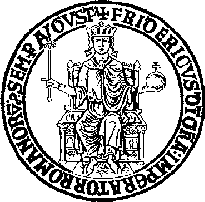
\includegraphics[width=3cm]{0_frontespizio/img/LogoFrontespizio}\\
	\vspace{3em}
	{\large\bfseries
	Dipartimento di Ingegneria Industriale\\
	\vspace{0.5em}
	Corso di Laurea in Ingegneria Meccanica\\
	\vspace{0.5em}
	Classe di Laurea LM-33\\ }
	\vspace{2em}
	{\Large
	\textsc{elaborato di laurea in}\\\vspace{1em}\textsc{riqualificazione energetica di edifici ospedalieri:\\ analisi progettuale relativa all'edificio 2\\ \vspace{0.3em}dell'aou~``Federico II''}}\\
	\vspace{5em}
	\begin{tabular}{p{8cm}l}
		\textbf{Relatori:}						&	\textbf{Candidato:}\\
		Ch.mo Prof. Ing. Adolfo Palombo 		&	Vincenzo Caccavale\\
		\tit{Ing.}{Annamaria Buonomano}			&	M65/646\\
		& \\
		\textbf{Correlatore:}					& 	\\
		\tit{Ing.}{Cesare Forzano}				& 	\\

	\end{tabular}
	\vfill
	Anno Accademico 2017/2018
\end{center}
\end{titlepage}
	\thispagestyle{empty}
\vspace*{5em}
\begin{center}
\large
Le arterie sono anarchiche\\ \vspace{0.05em} {\hspace{1.5cm}\small -- \tit{Dott.}{Giuseppe Sabino}}
\end{center}
	\thispagestyle{empty}
\vspace*{5em}
\begin{center}
\large
Le arterie sono anarchiche\\ \vspace{0.05em} {\hspace{1.5cm}\small -- \tit{Dott.}{Giuseppe Sabino}}
\end{center}
	\tableofcontents
\thispagestyle{empty}




	\begin{abstract}
L'Azienda Ospedaliera Universitaria ``Federico II'' è uno dei poli di riferimento in ambito ospedaliero e universitario di tutto il Mezzogiorno e rappresenta uno dei centri di più elevata specializzazione e qualificazione sul territorio nazionale. Operativa già dal 
1972, è costruita secondo uno schema a padiglioni che al giorno d'oggi risulta ancora completamente conservato. Le logiche e le idee alla base della sua progettazione, nonché della conseguente costruzione, ci sono state tramandate dall'\tit{Ing.}{Corrado Beguinot}, che all'epoca fu il direttore dei lavori. Con il procedere degli anni e con l'avvento di normative sempre più stringenti in ambito energetico, risulta evidente, se non scontato, riqualificare gli impianti meccanici e la struttura edilizia. In questo senso, il presente elaborato di laurea vuole essere un'analisi progettuale di un intervento di riqualificazione energetica da effettuarsi sull'edificio 2 di cardiochirurgia dell'AOU ``Federico II''.

Lo studio è stato condotto sfruttando ampiamente la tecnologia BIM che al giorno d'oggi sta prendendo sempre più piede in ambito progettistico. L'elevata flessibilità e cooperazione possibile solo con applicativi basati su questa filosofia, permette di migliorare notevolmente la qualità del prodotto nonché diminuire i tempi di esecuzione. A valle della modellazione termo-fisica dell'intero edificio, sono stati ricavati i carichi termici che hanno permesso inizialmente di individuare le criticità e successivamente di verificarne i risultati post-intervento. 

Il progetto prevede anche la costruzione di un impianto aeraulico e idronico per il controllo dei parametri termo-igrometrici all'interno dell'edificio 2: l'unico scopo è quello di migliorare il benessere per gli occupanti aumentando contemporaneamente la qualità dell'aria interna. Gli impianti sono stati anch'essi modellati e dimensionati all'interno di software BIM-based. A valle di tutto ciò segue la costruzione di una nuova sottocentrale in uno dei locali sotterranei dell'edificio 2. Si è fatto largo uso di macchine innovative che usufruiscono di energie rinnovabili: pompe di calore geotermiche e assorbitori bistadio che sfruttano i reflui termici del cogeneratore che altrimenti andrebbero persi in ambiente. A valle di tutta la progettazione è stata condotta un'analisi energetica per quantificare il risparmio e l'aumento di classe energetica secondo la normativa UNI~TS~11300.

%Tra tutte le strutture civili, quelle ospedaliere sono fra le più energivore. La causa principale va ricercata nelle particolari attività svolte, che richiedono grandi quantità di energia per poter garantire la miglior qualità di servizio agli utenti e per far fronte all'importante domanda di energia elettrica richiesta dalle apparecchiature e dagli strumenti diagnostici. Un'altra importante voce che incide sul bilancio energetico di un ospedale è costituita dalla climatizzazione degli ambienti, legata al raggiungimento e mantenimento delle elevate qualità dell'aria richieste per svolgere le attività sanitarie, si pensi alle particolari condizioni di asetticità richieste nei reparti operatori o nei locali dove sono assistiti i pazienti con patologie critiche. Occorre inoltre considerare l’approccio con cui
%molti degli ospedali oggi presenti nel nostro Paese sono stati costruiti. Nei decenni precedenti, grazie ai bassi costi dell'energia e soprattutto ad una minore sensibilità politica e sociale verso la sostenibilità economica ed ambientale delle attività umane, la progettazione e costruzione delle strutture sanitarie era orientata al raggiungimento degli standard sanitari richiesti, trascurando l’efficienza del sistema edificio-impianto.

%Da queste premesse appare evidente come i bilanci energetici degli ospedali, e più in generale delle strutture sanitarie, presentino elevati consumi elettrici e termici i cui costi ricadono nei bilanci economici delle aziende ospedaliere, e di conseguenza, vista l’elevata incidenza dei costi della sanità pubblica, sulle tasche dei cittadini/contribuenti. In questi tempi di crisi economica, di fronte alla sempre più impellente necessità di contenere la spesa pubblica e costi dei servizi ai cittadini, senza intaccare il livello qualitativo delle prestazioni erogate, la gestione energetica degli ospedali è una tra le innumerevoli voci di spesa la cui razionalizzazione è di fatto obbligatoria.
\end{abstract}	
	\thispagestyle{empty}
ringraziamenti 1\\
\newpage
\thispagestyle{empty}
ringraziamenti 2
%\begin{flushright}
%\Large\textsf{È fastidioso ringraziare solo in queste occasioni,\\bisognerebbe farlo più spesso.}	
%\end{flushright}
%
%I primi ``Grazie'' vanno ai miei genitori e alle mie sorelle che mi hanno sopportato per 26 anni\footnote{e continueranno a farlo!} e supportato soprattutto in questo ultimo periodo. Vi ringrazio per avermi ``inculcato'' l'amore per la curiosità che mi ha portato ad intraprendere la strada più azzeccata che abbia mai fatto in vita mia: ottenere un pezzo di carta con su scritto che sono ingegnere.
%
%Un saluto particolare al dottore e amico citato all'inizio di questa tesi: Giuseppe Sabino.
%
%Ringrazio gli ingegneri che mi hanno formato e permesso di arrivare in questo punto della mia carriera.\\
%Il \tit{Prof.}{Adolfo Palombo} per aver convogliato quel marasma di idee \emph{green} sull'efficientamento energetico in qualcosa di effettivamente utile;
%ringrazio Cesare Forzano e Annamaria Buonomano per la vostra gentilezza innanzitutto e poi per l'aiuto resomi disponibile alla fine\footnote{fine?} di questo percorso;
%ringrazio gli ingegneri Cristian Monfrecola e Lucio Pandolfi per avermi sottoposto ad una terapia forzata e necessaria di nonnismo!
%Ringrazio l'\tit{Ing.}{Gioacchino Forzano} per la sua umiltà e inspiegabilmente eccessiva disponibilità.\\
%Ringrazio tutto il gruppo ``Spuorchi e Scostumati'', ovvero la mia seconda famiglia. O dovrei ringraziare qualcuno ai piani alti per averci fatto incontrare? Sappiate che ognuno di voi è per me una spalla su cui piangere in caso di bisogno, una stanza vuota in cui sfogarmi, un panorama in cui rilassarsi, una compagnia per una passeggiata e una squadra (un po' scarsa!) di calcetto, siete una tavolata imbandita a pasquetta e un pieno di diesel per ogni viaggio, siete un bicchiere di vino per quando bisogna scherzare e un silenzio comprensivo, siete un caldo abbraccio e la corda giusta da pizzicare in un concerto. Vi voglio un mondo di bene e mi ritengo fortunato di avervi conosciuto! Un abbraccio particolare va ad Antonella, Ada, Nicola e Mario perché sì!\\
%A Roma e Pisa, invece, saluto il gruppo ``\emph{Ke sfaccimm la Kastla, il KKK, Wagliu e altre creature leggendarie}'' (ovvero i compagni Materazzo, Bucciarelli e Antonelli): siete la più inesauribile fonte di \emph{amicizia}. \\
%Ringrazio i miei amici Scout dell'Assoraider che considero da tempi immemori il mio rifugio tranquillo e disordinato dal rumore del mondo: un doveroso saluto va a Federica, Sara e Edoardo.
%\newpage
%\thispagestyle{empty}
%Ringrazio il gruppo dell'università per la stima che ci unisce, per il vostro sempre presente parere scientifico e per le burle: Biagio, Antonio, Gennaro, Pasquale, Giuseppe, Saverio e Luigi.\\
%Ringrazio, abbraccio e saluto tutto il resto della famiglia (nonni, zii, cugini, parenti vicini e lontani) perché siamo uniti e in contatto in ogni occasione anche se ci separano chilometri (e in alcuni casi \emph{migliaia} di chilometri).\\
%Saluto e ringrazio i miei professori del Liceo Scientifico "B. Pascal" di Pomezia per avermi mostrato, dimostrato e trasmesso nitidamente e a colori la passione per la cultura: \tit{Prof.ssa}{Cadelli}, \tit{Prof.}{Rossi}, \tit{Prof.ssa}{Nardecchia}, \tit{Prof.}{Russo} e la~\tit{Prof.ssa}{Zadra}.
%
%Ognuno di voi mi ha dato qualcosa a proprio modo e per questo vi ringrazio. Spero solo che almeno per un istante da quando vi conosco sia riuscito in qualche modo a ricambiare quanto mi avete dato.
%\vspace{2em}
%Lo studio presente in questo elaborato di laurea ha permesso sia di affacciarmi in prima persona al mondo del lavoro (ovvero applicare la teoria appresa all'università), sia di interfacciarmi con la macchina burocratica e con tutto quell'apparato di normative e leggi che, da una parte, consigliano e promuovono la \emph{retta via}, dall'altra, limitano e avviliscono l'operato umano privilegiando la mediocrità senza incoraggiare, invece, l'ingegno e la creatività che contraddistinguono un essere umano dall'altro.

%Consapevole di dovermi un giorno scontrare con poteri e logiche più forti di me, spero e mi
%auguro di avere sempre la forza di seguire le parole di \emph{Baden Powell}, fondatore dello scoutismo: ``\emph{Procurate di lasciare il mondo un po' migliore di come lo avete trovato}''.
%\vspace{1em}


	\mainmatter
	\chapter{La prima costruzione del Policlinico}
\thispagestyle{empty}
%\addcontentsline{toc}{section}{L'involucro}
%Si riportano stralci dei primi capitoli del III Volume \textsc{Ospedali e Cliniche Universitarie} dell'Ing. \textsc{Corrado Beguinot}. In questo modo, si spera di riuscire a evidenziare quelle che sono le differenze progettuali tra le normative vigenti all'epoca della costruzione del Policlinico e quelle odierne.\vspace{0.5em}
%Tutta questa parte scrivila con i margini più grandi, ovvero il testo deve essere più schiacciato orizzontalmente.
\begin{quoting}
	\emph{Con l'inizio dell'anno accademico 1972-73 la seconda Facoltà di Medicina e Chirurgia dell'\uni{} ha iniziato la sua attività nella sua nuova sede, all'epoca in parte ultimata ed in parte in corso di ultimazione.}
	
	\emph{Il numero degli studenti supera oggi le \num{6000} unità ed il numero complessivo dei letti è di \num{2758}.}

\emph{La Facoltà è costituita da un organismo edilizio articolato in ventisei edifici nei quali hanno sede gli Istituti, le Cliniche, i servizi e le attrezzature che sono collegati da gallerie di servizio a due livelli e da una viabilità principale e secondaria, e dotati di ampie superfici a verde e di parcheggi. La superficie complessiva su cui è stata realizzata la Facoltà è di \n{440000}{m^2} ed il volume costruito è di \n{11130000}{m^3} con una superficie totale dei piani pari a \n{270000}{m^2}.}

\emph{Il costo dell'opera, comprensivo del costo dei suoli, delle attrezzature didattiche, dell'arredo, delle sistemazioni esterne, degli impianti e degli oneri revisionali, è risultato di circa \num{45} miliardi con un costo quindi a \si{m^3} di \num{40000} lire circa.}

\emph{Gli istituti sono inseriti nei vari edifici in funzione delle loro affinità didattiche e di ricerca ed in funzione della prevista organizzazione dipartimentale.}

\end{quoting}
\noindent Le prime righe di questo elaborato di laurea sono state volutamente lasciate alle parole dell'\tit{ing.}{Corrado Beguinot} il quale coordinò i lavori di progettazione e costruzione del policlinico. 

Questo elaborato di laurea ha come obiettivo lo studio dell'Edificio 2 dell'AOU \uni{} (allora \emph{Patologia Medica}, ora \emph{Cardiochirurgia}) in vista di una sua riqualificazione energetica: sia per quanto riguarda l'involucro che gli impianti annessi. Volendo usare altre parole e riassumere molto banalmente il tutto, lo scopo di questo studio è quello di aumentare la classe energetica dell'edificio stesso. Il raggiungimento di questo obiettivo è iniziato con uno studio delle condizioni attuali dell'edificio. Sono stati effettuati vari sopralluoghi ma sopratutto si è cercato di recuperare materiale disponibile in letteratura. Sono risultati molto utili il terzo volume scritto dall'ingegnere Corrado Beguinot, di cui sono riportati i passi più utili, e l'analisi del \tit{prof.}{Adolfo Palombo} nel Giugno 2013 sugli edifici 9A, 9F e 9H. In questo modo è stato possibile ricavare dati preziosi riguardanti l'edificio 2 senza dover ricorrere ad analisi invasive delle pareti o coperture che comportano spese sicuramente economiche ma anche temporali.

Volendo entrare più nello specifico, si riportano gli stralci più importanti del suddetto terzo volume che hanno permesso di semplificare lo studio iniziale dell'edificio di patologia medica dell'AOU \uni. 

I primi passi, riportati all'inizio di questo capitolo, sono una spiegazione generica di come è stato concepito l'intero complesso ospedaliero. Andando avanti l'ingegnere si concentra sui corpi alti descrivendo la stratigrafia delle pareti verticali esterne e interne, gli infissi esterni (ovvero l'involucro trasparente) e quelli interni, per poi passare alle coperture. Seguono gli edifici bassi e i tunnel di collegamento. Dopo aver finito con la parte relativa all'architettura e all'edilizia si concentra sugli impianti utilizzati.\\
Inerentemente all'edificio 2, il Beguinot si esprime così:
\begin{quoting}
	L'edificio di \emph{Patologia Medica} comprende\emph{: laboratori di ricerca e stabulari per una superficie di circa \n{1200}{m^2}; 1 aula da \num{400} posti, \num{8} aule da \num{30} in comune con la Semeiotica Medica, l'Endocrinologia e la Dermatologia; reparti di degenza per un totale di \num{150} posti-letto, con una superficie di circa \n{4400}{m^2}. La superficie totale dei piani è di \n{8700}{m^2} circa.}
\end{quoting}
Per quanto riguarda l'involucro opaco e trasparente, invece:
\begin{quoting}
	\emph{L'adozione di un sistema modulare generale ha consentito una impostazione unitaria della costruzione dei complessi delle Cliniche, costituiti dai corpi alti delle degenze e dai corpi delle piastre di base degli ambulatori, delle diagnostiche, degli uffici, dei laboratori, delle aule, ecc.}
	
	\emph{La struttura dei corpi di degenza è essenzialmente costituita da una teoria perimetrale di pilastri pressoinflessi, posti ad interasse di \n{1.90}{m}, collegati ai piani da un solaio c.a. realizzato con coppie di travi a sezione rettangolare, agganciate lateralmente ai pilastri, e solette piene in calcestruzzo. La rigidezza globale del sistema è assicurata da una trave perimetrale parapetto e dai blocchi dei collegamenti verticali, scala principale, scale di servizio e di emergenza, costituiti da pareti portanti in c.a. dello spessore di \n{40}{cm}, dalle quali escono a sbalzo i gradini prefabbricati ed i ripiani. Il coronamento dell'edificio è realizzato con elementi modulari prefabbricati in c.a., agganciati al prolungamento dei pilastri.}

\sdots

	\emph{Le facciate dei corpi degenza sono caratterizzate, oltre che dagli elementi pieni di calcestruzzo armato dei collegamenti verticali, da una alternanza di pieni e vuoti, realizzati con l'adozione di un elemento tipo prefabbricato, di lunghezza modulare, ancorato mediante piastre, perni e bulloni ai pilastri. I suddetti blocchi sono costituiti da un doppio strato di silicalcite pesante e leggera, e sono rifiniti sulla faccia esterna con una superficie granigliata e sul lato interno a stucco. Lo spazio libero, tra la fascia parapetto e l'intradosso del solaio, è modulato in sette parti uguali, che sono occupate da elementi prefabbricati o elementi di infisso in accordo con le esigenze di visibilità e di illuminazione degli ambienti interni e della composizione della superficie esterna.}

\sdots

	\emph{Allo scopo di attenuare la rumorosità negli ambienti sono stati adottati nei corridoi e nelle altre zone di traffico (atrio al piano, soggiorno pazienti, testate di servizio) pavimenti di gomma; nelle camere di degenza, nei soggiorni per i visitatori, e negli studi si è adottata una pavimentazione resiliente. Sia i pavimenti di gomma che quelli resilienti sono posti in opera su sottofondo di arena e cemento. In tutti i locali di servizio, in quelli soggetti a più frequenti lavaggi e disinfezioni, cioè ambienti per la visita medica, laboratori, ecc., si è adottata una pavimentazione in grés opaco.}

\sdots

	\emph{Per l'alloggiamento degli impianti sono stati predisposti nelle strutture appositi cavedi, ubicati in posizione tali da servire in maniera omogenea la superficie di ogni piano. Più precisamente sono stati realizzati due grandi cavedi in corrispondenza rispettivamente della scala di sicurezza all'estremità del corpo di fabbrica e del torrino dei servizi, che è anche attraversato verticalmente da altri tre cavedi più piccoli, dei quali due per impianti idrico-sanitari ed uno di forma allungata, riservato esclusivamente agli impianti elettrici. Una serie continua di cavedi attraversa longitudinalmente tutto il corpo della degenza, accogliendo le condotte pluviali, gli scarichi degli impianti idrici annessi alle camere di degenza, le canne di aspirazione delle cappe dei laboratori, nei casi in cui è prevista l'ubicazione di questi ultimi nel piano rialzato del blocco degenza, e le reti di distribuzione dei gas medicali.}

\sdots

	\emph{I cavedi, grandi e piccoli, ed ogni altra canalizzazione verticale, al piano cantinato, fanno capo alle reti orizzontali, ospitate nella galleria di servizio.}
	
	\emph{L'isolamento termico delle coperture è ottenuto con l'interposizione, tra solaio ed impermeabilizzazione, di uno strato coibente, sul quale è disposto un masso concreto con pendenza verso l'interno del corpo di fabbrica per il raccordo delle pluviali, sistemate nei cavedi precedentemente descritti.}

\sdots

	\emph{Gli infissi esterni sono realizzati con profilo in lamierino di acciaio verniciato a fuoco e vetro semidoppio; quelli delle camere di degenza, alternati con i blocchi di silicalcite, hanno apertura a vasistas e tenda di oscuramento in tessuto plastico; quelli del torrino dei servizi e dell'atrio di piano realizzano una fascia continua verticale, interrotta solo dallo spessore dei solai e dalla fascia parapetto, ed hanno apertura a battente.}

\sdots

	\emph{Per quanto riguarda la finitura delle superfici interne ed esterne si ricorda che sono lasciati a vista i getti di calcestruzzo sia all'interno che all'esterno, proteggendoli con vernice idrorepellente ed antipolvere. Le altre pareti ed i soffitti sono dipinti con pittura lavabile. In particolare quelle delle camere di degenza, realizzati, come già detto con solette e travi binate, hanno il calcestruzzo a vista per le travi e l'intradosso delle solette, gettate su cassaforma di compensato marino, semplicemente stuccate e dipinte con pittura lavabile.}
\end{quoting}
\noindent I corpi bassi differiscono di poco dalla struttura modulare di quelli alti. Infatti:
\begin{quoting}
	\emph{La struttura portante dei corpi bassi conserva la stessa modulazione dei blocchi degenze.}

\sdots

	\emph{La trave parete, oltre alla funzione di collegamento e di irrigidimento dell'insieme, ha anche quella di contenimento del terreno per il piano di servizio che corre continuo alle piastre.}
	
	\emph{Le coperture di tali corpi sono realizzate con elementi in cemento armato ad U capovolto, sul modulo tipo di \n{1.90}{m}, poggiati su travi portanti longitudinali, ed uscenti a sbalzo per \n{1.60}{m}, onde realizzare una zona d'ombra sulle pareti verticali.}

\sdots

	\emph{Uno strato coibente ed un'impermeabilizzazione a guaina sintetica proteggono le coperture, seguendone il profilo grecato.}

\sdots

	\emph{Le facciate esterne sono costituite dall'alternanza di elementi di tompagno e di infissi, suggerita dalla funzionalità esterna.}
	
	\emph{I tompagni sono realizzati con doppia fodera: pannello prefabbricato di cemento granigliato all'esterno, e tavolato di mattoni forati intonacato all'interno. Gli infissi sono in lamiera di acciaio verniciato a fuoco di tipo analogo a quelli del corpo di fabbrica delle degenze.}
\end{quoting}

%\addcontentsline{toc}{section}{L'impianto}
\noindent Per quanto riguarda la parte impiantistica si vogliono riportare ancora stralci de \emph{Ospedali e Cliniche universitarie} scritto dall'\tit{Ing.}{Corrado Beguinot}: si tratta in questo caso del secondo capitolo che ha come titolo ‘‘\emph{Gli Impianti Termofrigoriferi~-~\emph{Centrale Termofrigorifera, Sottocentrali ed Impianti Interni}}''.
\begin{quoting}
	\textbf{Centrale Termofrigorifera} -- \emph{La Centrale Termofrigorifera, ubicata nell'area delle attrezzature centralizzata, è stata realizzata dalla Marelli Aerotecnica} \dots
		
\sdots 
	
	\emph{L'edificio della Centrale occupa un'area di \n{2850}{m^2} con un volume entrofuoriterra pari a \n{21000}{m^3}. È realizzato con strutture in cemento armato a faccia a vista e con tecnologie analoghe a quelle prevalenti nel complesso Policlinico e, in particolare, per gli impianti tecnologici centralizzati.}
	
	\emph{L'opera realizzata dalla Marelli afferma il principio della centralizzazione della produzione del caldo e del freddo per tutte le utenze relative ai molteplici Istituti e Servizi. I vantaggi del sistema adottato possono condensarsi nei seguenti punti: minor potenzialità installata, riserva a costi minori, impiego di combustibili densi ed eventuale utilizzazione futura del gas metano, concentrazione stoccaggio combustibili con minori costi, maggiore durata con rendimenti più alti, minori investimenti con minori costi di manutenzione, minori consumi d'acqua con minori costi di produzione, riduzione delle fonti di inquinamento.}
	
	\emph{Nella Centrale Termofrigorifera sono state installate: 5 caldaie con una potenzialità complessiva di circa \n{60d6}{kcal/h}, 5 gruppi frigoriferi, di cui uno del tipo ad assorbimento avente una capacità di \n{3d6}{frig/h}\footnote{Si ricorda che la \emph{frigoria} è l'opposto di una \emph{caloria}. Pertanto \n{d6}{frig/h} equivalgono a circa \n{116.3}{kW}} e 4 di tipo Centrifugo con capacità singola di \n{6d6}{frig/h}. Le caldaie forniscono vapore surriscaldato, sia per la produzione di acqua surriscaldata delle sottocentrali, quanto per l'azionamento delle turbine collegate ai gruppi frigoriferi centrifughi e delle turbopompe di circolazione dei fluidi prodotti dall'impianto frigorifero (acqua refrigerata e acqua raffreddamento condensatori).}
	
	\emph{Le caldaie sono del tipo pressurizzato e collegate ognuna ad un recuperatore per il massimo sfruttamento del calore sensibile dei prodotti della combustione.}
	
	\emph{Ogni caldaia produce vapore alla pressione di \n{40}{kg/cm^2} surriscaldato a circa \n{360}{\degreeCelsius}.}
	
	\emph{L'energia termica, sia per il periodo invernale come per il periodo estivo, per il riscaldamento e produzione acqua calda necessaria ai servizi, viene distribuita mediante acqua surriscaldata ad una temperatura di circa \n{170}{\degreeCelsius}, non oltre i \n{180}{\degreeCelsius}.}
	
	\sdots
	
	\emph{La circolazione dell'acqua surriscaldata è assicurata da più pompe elettrocentrifughe che, attraverso un'estesa rete di distribuzone, servono ogni fabbisogno termico attraverso scambiatori installati nelle varie sottostazioni dislocate negli scantinati dei divers fabbricati.}
	
	\emph{La Centrale Termica è integrata da un impianto di trattamento di acqua grezza, sia per il riempimento del sistema acqua surriscaldata, sia per il reintegro spurghi caldaie.}
	
	\emph{Affiancata alla Centrale Termica, ma divisa, in rispetto delle norme VV.FF., è stata realizzata la Centrale Frigorifera con una serie di 4 gruppi centrifughi in parallelo ed uno ad assorbimento; i primi, azionati da turbine in contropressione, mentre l'assorbitore utilizza, in parte, il vapore di scarico delle turbopompe di circolazione dell'acqua di condensazione refrigerata.}
	
	\emph{L'adozione della macchina ad assorbimento è stata attuata per potere sfruttare meglio il vapore e poter far funzionare gli impianti primari e secondari in modo soddisfacente anche a bassi carichi continui (funzionamenti notturni, periodo invernale), in modo che possa essere tenuto in funzione il maggior numero di ore/anno in relazione alle fluttuazioni dei carichi dal 100\% alle minime percentuali con i più elevati rendimenti, e con semplice regolazione.}
	
	\emph{Il vapore ad alta pressione ed alta temperatura, proveniente dalle caldaie, viene distribuito in parallelo: alle quattro turbine a condensazione, accoppiate direttamente ai quattro compressori centrifughi, ai quattro turboriduttori a contropressione delle pompe di circolazione dell'acqua di raffreddamento dei condensatori e circolazione dell'acqua refrigerata.}
	
	\sdots
	
	\emph{Data la notevole quantità d'acqua necessaria al raffreddamento dei condensatori dei gruppi centrifughi, dell'assorbitore e condensatori dell'utilizzo vapore al fine di limitare i consumi, l'acqua di raffreddamento è inviata a un complesso di torri di raffreddamento che la riporta ad una temperatura di utilizzo per uno sfruttamento in ciclo chiuso. La torre, che nel suo assieme è costituita da otto torri con otto bacini di raccolta acqua, realizzati in cemento armato, ha una lunghezza di 50 metri, larga 10 metri ed oltre 15 metri in altezza; tratta \n{6000}{m^3/h} di acqua per una potenzialità di scambio pari ad oltre 45 milioni di \si{cal/h}.}
\end{quoting}
Alla fine del capitolo viene riassunto il funzionamento di ogni sottocentrale presente nello scantinato di ogni corpo di fabbrica.
\begin{quoting}
	\textbf{Sottocentrali} - \emph{Tutte le sottocentrali sono collegate alla rete primaria dell'acqua surriscaldata la quale cede il proprio carico termico  al circuito secondario a mezzo di scambiatori di calore di tipo acqua-acqua.}
	
	\emph{I due regimi idraulici dei due fluidi, del primario e del secondario, sono così indipendenti.}
	
	\emph{L'eventuale esclusione del circuito secondario e la sua parzializzazione è permessa by-passando l'acqua attraverso una valvola a tre vie, rimanendo così costante la portata d'acqua nella rete primaria.}
	
	\emph{L'acqua surriscaldata soddisfa pure i fabbisogni termici per i servizi igienici alimentando i collettori; sono previsti tutti gli accorgimenti onde garantire la sicurezza del servizio.}
	
	\emph{Per l'acqua refrigerata invece il circuito primario è collegato direttamente alle reti secondarie attraverso valvole miscelatrici; pertanto i due circuiti, primario e secondario, sono collegati idraulicamente.}

\sdots


\noindent\emph{Le sottocentrali e gli impianti interni degli istituti clinici comprendono:}	
\begin{enumerate}
	\item Sottostazioni di produzione del calore;
	\item Sottostazioni di produzione del freddo;
	\item Quadri elettrici e regolazioni automatiche;
	\item Distribuzione del calore e del freddo;
	\item Condizionamento dell'aria;
	\item Riscaldamento a piastre;
	\item Estrazione aria viziata servizi degenze;
	\item Produzione e distribuzione dell'aria compressa;
	\item Produzione e distribuzione del vuoto;
	\item Distribuzione del gas illuminante;
\end{enumerate}
\subsubsection{Sottostazione di produzione del calore}
\emph{Le sottostazioni realizzate sono:}
\begin{itemize}
	\item Medicina Generale
	\item Semeiotica Medica
	\item Patologia Medica
	\item Medicina del Lavoro
	\item Ostetrica e Ginecologica
	\item Radiologia
	\item Pediatrica e Puericultura
	\item Malattie Nervose e Mentali
	\item Malattie Infettive
	\item Ortopedica
	\item Otorino
	\item Odontoiatrica
	\item Neurochirugica
	\item Chirurgia Generale
\end{itemize}
\vspace{0.5em}
	\noindent\emph{In ciascuna delle predette sottostazioni sono state installate le apparecchiature di trasformazione del calore costituite, per ognuna, da due scambiatori per la produzione di acqua calda a \num{90}} + \emph{\num{95}\si{\degreeCelsius} e due scambiatori per la produzione dell'acqua calda a \n{60}{\degreeCelsius}.}
	
	\emph{Gli scambiatori sono alimentati dal fluido primario costituito da acqua surriscaldata proveniente dai distributori correnti nel cunicolo alla temperatura di circa \n{170}{\degreeCelsius} e con ritorno di \n{110}{\degreeCelsius}, con una pressione disponibile tra andata e ritorno di 10 metri di colonna d'acqua.}
	
	\emph{Ogni scambiatore è dotato di propria apparecchiatura di termoregolazione automatica, a funzionamento pneumatico, costituito essenzialmente da valvola deviatrice a tre vie, comandata da termostato posto sulla scia del secondario.}
	
	\emph{Sono state installate nelle stesse sottocentrali i collettori di andata e ritorno dell'acqua calda alle diverse temperature e le relative elettropompe di circolazione; sono stati inoltre installati i dispositivi necessari per mantenere costante la pressione dell'acqua surriscaldata in arrivo alle sottostazioni.}
	
	\emph{Tutte le apparecchiature delle sottostazioni sono state superdimensionate per tener conto di eventuali futuri fabbisogni termici.}
	\subsubsection{Sottostazioni di produzione del freddo}
	\emph{Negli stessi locali sono stati portati gli allacciamenti dell'acqua refrigerata di circa \n{4}{\degreeCelsius} in arrivo e ritorno a \n{12}{\degreeCelsius}. Per ciascuna sottostazione è stata prevista un'apparecchiatura regolatrice, stabilizzatrice di pressione, ed un contatore di frigorie con totalizzatore settimanale. È stata inoltre posta un'apparecchiatura di regolazione automatica atta a mantenere costante la temperatura di ritorno a \n{12}{\degreeCelsius}.}

	\sdots
	\subsubsection{Distribuzione del calore e del freddo}
	\emph{Dai collettori posti nelle sottostazioni partono le tubazioni di trasporto dell'acqua calda e fredda per l'alimentazione dei vari impianti di condizionamento e di riscaldamento.}
	
	\emph{Queste reti sono state realizzate in tubi di acciaio trafilato <<Mannesmann>>, posti in opera mediante saldature ossiacetileniche, verniciate antiruggine ed isolate termicamente; completano le reti le saracinesche d'intercettazione.}
	\subsubsection{Condizionamento dell'aria}
	\emph{Molteplici sono i tipi d'impianti realizzati nelle varie Cliniche e precisamente: per i locali adibiti ad uffici e laboratori sono stati realizzati impianti <<ad induzione>> con aria primaria atta ad assicurare un ricambio di circa \n{2}{Vol/h}.}
	
	\emph{Altro tipo di impianto è stato quello a doppio condotto ad alta velocità con cassette miscelatrici-attenuatrici e l'alimentazione delle bocchette a bassa velocità; ciascuna cassetta miscelatrice è comandata da termostato in ambiente. Gli ambienti sono condizionati a tutt'aria esterna ed i ricambi di aria sono stati determinati in funzione dei carichi termici e delle necessità di ventilazione dovuta ai particolari usi a cui i locali stessi sono stati adibiti.}

	\emph{Ciascun impianto di condizionamento si completa con l'impianto di estrazione dell'aria con smaltimento diretto all'esterno.}
	
	\emph{Gli stabulari ed i locali delle terapie sono stati trattati con impianti indipendenti del tipo convenzionale a tutt'aria esterna.}
	
	\emph{I ricambi assicurati sono pari ad almeno \n{12}{Vol/h}.}
	
	\sdots
	\subsubsection{Riscaldamento a piastre}
	\emph{Nei locali degenze e servizi sono stati realizzati impianti di riscaldamento con termoconvettori in prevalenza in alluminio pressofuso. In questi ambienti la temperatura garantita è di \n{20}{\degreeCelsius}, anche in relazione alla minima esterna invernale di \n{0}{\degreeCelsius}.}
	
	\sdots
	
	\emph{Ciascuna colonna montante o discendente dell'impianto di riscaldamento è dotata di saracinesche d'intercettazione in bronzo pesante con rubinetti di scarico a maschio, con attacco portagomma sul ritorno.}
	
	\emph{Per ogni corpo di fabbrica è stato previsto un circuito diverso intercettabile con saracinesche nella sottostazione.}
	\subsubsection{Estrazione aria viziata dei servizi degenze}
	\emph{Per questi impianti sono state installate bocchette di ripresa a portata regolabile in maniera da permettere di regolare perfettamente la portata di aria ripresa nel singolo ambiente. Esse fanno capo ad una canalizzazione verticale in lamiera di ferro zincato prolungata fino alla copertura e collegata ad un collettore di raccolta dell'aria da smaltire, facente capo ad un ventilatore di espulsione dell'aria viziata.}
\end{quoting}



	%\chapter{Descrizione del bando}
\thispagestyle{empty}
In attesa\dots NON HO IL BANDO
	\chapter{Teoria sulla climatizzazione degli edifici}
\thispagestyle{empty}
L'essere umano ha il continuo desiderio di vivere un luogo in condizioni termo-igrometriche perfette. 

La teoria che si cela dietro l'attributo \emph{termo-igrometrico} è alla base della climatizzazione degli edifici.

Cosa si intende per \emph{climatizzazione}? Un edificio si definisce climatizzato o un impianto è di climatizzazione quando vengono controllati questi valori ambientali:
\begin{itemize}
	\item Temperatura;
	\item Umidità;
	\item Qualità dell'aria mediante un suo ricambio.
\end{itemize}
Il controllo di questi tre valori permette di vivere, come già è stato detto, un ambiente in condizioni termo-igrometriche ottimali. E solo un impianto di climatizzazione (solitamente un UTA -- \emph{Unità di Trattamento dell'Aria}) propriamente detto permette di ottenere questi risultati. Se, per esempio, non viene garantito il ricambio dell'aria (ovvero non viene immessa in ambiente una certa portata di aria esterna), l'impianto non è di climatizzazione. A tal proposito, i mono-split a compressione di vapore che abbiamo nelle nostre case non sono \emph{climatizzatori} ma dei semplici \emph{raffrescatori} (o \emph{riscaldatori} a seconda della stagione).

La domanda successiva a cui bisogna dare una risposta è la seguente: \emph{quali sono le condizioni termo-igrometriche ottimali?}

La risposta è complicata anche se alcuni progettisti termo-tecnici tenderebbero subito a rispondere: \n{25}{\degreeCelsius} col \n{40}{\%} in estate e \n{20}{\degreeCelsius} col \n{50}{\%} in inverno.

In verità, per rispondere concretamente a questa domanda bisogna introdurre la teoria sulla climatizzazione degli edifici. E per farlo si parte dal soggetto del primo periodo di questo capitolo: \emph{l'essere umano}.

\section{Il Comfort}
L'uomo, in quanto essere vivente, trasforma continuamente l'energia chimica presente negli alimenti in forme più consone al mantenimento in vita del proprio corpo e alla sua trasformazione: quest'attività prende il nome di \emph{metabolismo}.

Questa continua trasformazione produce calore che risulta variabile in base all'attività svolta: stare seduto, camminare, correre, fare attività pesante e così via.

Non è difficile concludere che, considerando l'essere umano come un sistema chiuso, questo calore prodotto produce un accrescimento della temperatura corporea. Idealmente fino all'infinito. Ovviamente, l'essere umano non è un sistema chiuso e questo calore interno deve essere smaltito in relazione alle condizioni climatiche dell'ambiente esterno e, contemporaneamente, deve garantire la temperatura interna corporea.

In termini matematici il tutto si traduce in questo bilancio di potenze
\begin{equation}
	\label{bilanciocorpoumano}
	S=M-W-E_d-E_{sw}-E_{ve}-C_{ve}-C-R-C_k
\end{equation}
dove:
\begin{description}
	\item[$\mathbf{S}$]Variazione di energia del corpo umano nell'unità di tempo o accumulo di energia termica nell'unità di tempo;
	\item[$\mathbf{M}$]Potenza metabolica;
	\item[$\mathbf{E_d}$] Potenza termica dispersa per diffusione attraverso la pelle;
	\item[$\mathbf{E_{sw}}$] Potenza termica dispersa per sudorazione attraverso la pelle;
	\item[$\mathbf{E_{ve}}$] Potenza termica dispersa nella respirazione come "calore latente";
	\item[$\mathbf{C_{ve}}$] Potenza termica dispersa nella respirazione come "calore sensibile";
	\item[$\mathbf{C}$] Potenza termica dispersa per convezione;
	\item[$\mathbf{R}$] Potenza termica dispersa per irraggiamento;
	\item[$\mathbf{C_k}$] Potenza dispersa per conduzione;
\end{description}
È risaputo che nel caso in cui la temperatura esterna sia eccessivamente alta o bassa, il meccanismo termoregolatorio del corpo tenda rispettivamente a far sudare il corpo stesso (smaltendo il calore tramite evaporazione del sudore) o a provocare i brividi (aumento dell'attività muscolare e quindi di calore prodotto). Nel caso in cui questi due ultimi meccanismi non siano sufficienti a mantenere costante l'energia interna del corpo si ha l'\emph{ipertermia} (fino alla morte per danni reversibili alle proteine dei tessuti nervosi) o l'\emph{ipotermia} (fino alla morte per fibrillazione cardiaca).

Quindi, è molto importante vivere in un ambiente che abbia delle condizioni termo-igrometriche tali da non provocare la morte prematura del proprio corpo.

Il vero problema è che queste così agognate \emph{condizioni termo-igrometriche ideali} non sono universali. E il motivo risiede nel fatto che ogni persona è diversa dalle altre. Infatti, ognuno tende a vestirsi diversamente (ovvero cambia la resistenza termica che il corpo oppone verso l'esterno e contemporaneamente anche il suo fattore di vista nel caso dell'irraggiamento) ma sopratutto ognuno tende ad avere un'attività metabolica $M$ completamente diversa. È come se ogni persona desiderasse una propria temperatura. Ovviamente è praticamente impossibile realizzare una cosa del genere in un ambiente affollato.

Citando da \emph{Impianti di climatizzazione per l'edilizia}~\cite{alfano}:
\begin{quote}
	Perché ci sia comfort termico, una condizione necessaria è che l'energia interna del corpo umano non aumenti nè diminuisca, ovvero che sia nullo il termine di accumulo che nella \ref{bilanciocorpoumano} è indicato come $S$; per $S=0$ questa equazione diventa una relazione del tipo:
	\begin{equation}
	\label{bilanciocorpoumanoSnullo}
		f(\mathrm{abbigliamento, attivit\grave{a}}, t_a, v_a, \Phi, t_r, t_{sk}, E_{sw})=0
	\end{equation}
	che lega tra loro otto variabili: due legate al soggetto (abbigliamento e attività), quattro ambientali (temperatura $t_a$, velocità $v_a$ e umidità~$\Phi$ dell'aria e temperatura media radiante $t_r$ -- ovvero temperatura di un ambiente fittizio termicamente uniforme che scambierebbe con l'uomo la stessa potenza termica radiante scambiata nell'ambiente reale) e due fisiologiche (temperatura della pelle $t_{sk}$ e potenza termica dispersa per sudorazione o percentuale di pelle bagnata dal sudore $E_{sw}$).
	
	In verità le due variabili fisiologiche non sono variabili indipendenti, ma dipendono con legge complessa dalle altre; 
	
	\sdots
	
	Secondo Fanger, perché siano verificate le condizioni di benessere, devono essere anche soddisfatte le due equazioni:
	\begin{gather}
	\label{Esw}
		E_{sw}=0.42A_b[(M-W)/A_b-58.2]\\
	\label{tsk}
		t_{sk}=35.7-0.0275(M-W)/A_b
	\end{gather}
	cioè i valori di $E_{sw}$ e di $t_{sk}$ reali in condizioni di comfort termico sono quelli che si ottengono dalle due ora scritte in funzione dell'attività realmente svolta dal soggetto.
	
	In definitiva le possibili condizioni di benessere termico sono le combinazioni delle sei variabili indipendenti che soddisfano contemporaneamente le equazioni \ref{bilanciocorpoumanoSnullo}, \ref{Esw} e la \ref{tsk}.
\end{quote}
Col tempo sono stati definiti degli indici che permettono di valutare il benessere termico in un locale. 

Uno di questi è il PMV (\emph{Predicted Mean Vote} -- Voto Medio Previsto): indipendentemente dal valore assunto dalle 6 variabili indipendenti, se 
\begin{equation}
\label{PMV}
	-0.5<\textrm{PMV}<0.5
\end{equation}
allora una condizione necessaria ma non sufficiente per il benessere è soddisfatta.

L'altra condizione che permette di vivere in un ambiente termicamente accettabile è l'assenza di \emph{discomfort localizzato}, causato da:
\begin{itemize}
	\item elevati gradienti verticali e orizzontali di temperatura;
	\item correnti d'aria.
\end{itemize}
Per tutte queste cause vi sono altrettanti indici che permettono di esprimere la presenza o meno di problematiche.

Quindi riassumendo: nel momento in cui le cause di discomfort localizzato sono assenti e il valore del PMV (che è un indice di discomfort \emph{globale} perché interessa tutto l'ambiente) è compreso nel suddetto intervallo (\ref{PMV}), allora l'ambiente stesso si può definire termo-igrometricamente accettabile. 

Per concludere questa parte sul comfort è bene precisare che, citando da \emph{Impianti di climatizzazione per l'edilizia}~\cite[pag 31]{alfano}
\begin{quote}
	gli indici esprimono la risposta media di un gran numero di soggetti, il che significa che per valori dell'indice corrispondenti per esempio a condizioni di comfort termico ci possono comunque essere individui che invece avvertono caldo o freddo.
\end{quote} 
È chiaro, quindi, che per ogni tipologia di locale (in cui verosimilmente le persone svolgono attività comuni) sono definiti dei valori che permettono di assicurare le condizioni di benessere. Solitamente, comunque, a meno di casi eccezionali in cui sono necessarie condizioni termiche altrettanto particolari, gli ambienti o i locali in cui le persone svolgono attività leggere, vestiti \emph{normalmente}\footnote{È in corsivo perché anche il vestiario è normato e quindi un capo di abbigliamento è diverso dall'altro e produce risultati diversi: non esiste un vestito \emph{normale}. Con questo termine mi riferisco, quindi, ad una tipologia di vestiario comune.} (quindi uffici e similari), in cui non si suda, i valori di temperatura e umidità sono quasi sempre quelli enunciati all'inizio di questo capitolo: \n{25}{\degreeCelsius} col \n{40}{\%} in estate e \n{20}{\degreeCelsius} col \n{50}{\%} in inverno.
\section{Il Carico Termico}
Dopo aver definito il comfort in un ambiente, è necessario calcolare il carico termico che consente di dimensionare l'impianto che permetta di realizzare quelle condizioni termo-igrometricamente accettabili di cui si è parlato nel paragrafo precedente.

\subsection{Carico Termico Invernale}
Con \emph{carico termico invernale} si definisce una potenza termica che l'edificio, in precisate condizioni univocamente definite, disperde verso l'ambiente esterno. Le suddette \emph{condizioni definite} sono:
\begin{itemize}
	\item il clima, ovvero i \emph{parametri climatici esterni} che costituiscono le sollecitazioni esterne sul sistema edificio. Questi parametri sono di disturbo perchè allontanano le condizioni termiche dell'ambiente interno da quelle desiderate di benessere. Queste cause sono:
	\begin{itemize}
		\item la differenza di temperatura tra l'aria interna e quella esterna;
		\item il vento che investe l'edificio;
		\item la radiazione solare incidente.
	\end{itemize}
	Per una valutazione approssimativa del carico termico invernale, è essenziale conoscere perlomeno la differenza di temperatura tra interno e esterno. La velocità dell'aria, invece, è importante se si vuole considerare anche lo scambio termico convettivo. L'apporto solare non viene considerato nel carico invernale in quanto è un beneficio perché tende a riscaldare l'ambiente interno e quindi, per questioni di sicurezza, viene ignorato;
	\item l'edificio, inteso come involucro edilizio che racchiude e delimita lo spazio interno nel quale si vogliono imporre le condizioni di benessere per gli occupanti, diventa così il confine fisico tra esterno ed interno e caratterizza fortemente l'interazione termica tra i due ambienti con le sue proprietà geometriche e termofisiche. Progettare un impianto di riscaldamento significa quindi mettere a punto un sistema capace di neutralizzare nell'ambiente interno gli effetti prodotti prevalentemente dal clima esterno;
	\item l'impianto è lo strumento con cui mantenere nell'ambiente riscaldato le condizioni volute contrastando le perturbazioni indotte dalle variazioni climatiche esterne.
\end{itemize}
La trattazione sui carichi termici invernali non si occupa degli aspetti igrometrici e di quant'altro attiene al vapor d'acqua, si affrontano cioè le sole problematiche legate al cosiddetto \emph{calore sensibile}, ossia agli scambi di calore che manifestano i loro effetti sulla sola temperatura di bulbo asciutto dell'aria esterna.

Da un'analisi energetica sull'edificio, si ricava la seguente relazione:
\begin{equation}
	\dot{Q}_{\textrm{risc}}=\dot{Q}_T+\dot{Q}_V-\dot{Q}_{\textrm{sor}}-\dot{Q}_{\textrm{sol}}
\end{equation}
Solitamente non potendo confidare con certezza in tutta la stagione negli apporti gratuiti interni $\dot{Q}_{\textrm{sor}}$ e solare $\dot{Q}_{\textrm{sol}}$ nell'equazione che definisce il carico termico invernale questi ultimi vengono trascurati. Per cui il \emph{carico termico invernale} è definito attraverso la seguente relazione:
\begin{equation}
\label{caricotermico:invernale}
\dot{Q}_{\textrm{risc}}=\dot{Q}_T+\dot{Q}_V+\dot{Q}_{\textrm{ripr}}
\end{equation}
dove $\dot{Q}_T$ è il carico termico invernale dovuto alla trasmissione tramite l'involucro dell'edificio e $\dot{Q}_V$ è quello dovuto al riscaldamento dell'aria immessa (con un impianto di ventilazione o tramite semplice infiltrazione naturale) all'interno dell'edificio stesso per portarlo alle condizioni desiderate di progetto. L'ultimo termine viene introdotto in quanto, secondo la \norinv\ sugli \emph{Impianti di riscaldamento negli edifici -- Metodo di calcolo del carico termico di progetto} serve a tener conto della potenza termica aggiuntiva, detta di \emph{ripresa}, necessaria a compensare gli effetti del regime intermittente dell'impianto di riscaldamento.

Il calcolo del carico termico invernale si fonda su tre ipotesi:
\begin{itemize}
	\item Trascurabilità degli apporti gratuiti: ovvero non si considera la $\dot{Q}_{\textrm{sor}}$ e la $\dot{Q}_{\textrm{sol}}$;
	\item Condizione statisticamente più sfavorevole: in questo modo l'impianto sarà sempre in grado di mantenere le condizioni di benessere all'interno dell'edificio;
	\item Regime stazionario: la principale grandezza climatica che ha la capacità di produrre un regime transitorio nell'edificio è la radiazione solare che si è detta trascurabile in inverno.
\end{itemize}

In base alla norma \norinv, la $t_e$ è la temperatura dell'aria esterna di progetto del luogo ove è ubicato l'edificio in esame ed è necessaria per il calcolo della $\dot{Q}_{\textrm{risc}}$. L'ipotesi di \emph{regime stazionario} obbliga a scegliere per il calcolo delle dispersioni una temperatura dell'aria esterna che sia costante (quando evidentemente non lo è perché si tratta di un parametro climatico) e che sia caratteristica delle condizioni meteorologiche del luogo e del clima in cui sorge l'edificio oggetto del calcolo. L'ipotesi delle \emph{condizioni più sfavorevoli} porterebbe a scegliere una temperatura che sia la più bassa tra quelle che stagionalmente si verificano nel corso degli anni nella località in cui l'edificio si trova. Solo in questo caso si sarebbe sicuri di calcolare un carico di picco per l'impianto sufficiente a garantire nell'ambiente riscaldato la temperatura $t_i$ anche al presentarsi delle sollecitazioni esterne più avverse.

Il problema con la seconda ipotesi risiede nel fatto che se si considera la temperatura più bassa degli ultimi, per esempio, 10 anni, si andrebbe a costruire un impianto molto sovradimensionato in quanto quella stessa temperatura potrebbe non aversi per alcuni anni e nel frattempo l'impianto non verrebbe sfruttato al 100\%. 

Proprio per queste ragioni l'ipotesi di \emph{condizioni più sfavorevoli} va in generale coniugata alle esigenze pratiche ed economiche. A tale scopo per stabilire la temperatura esterna di progetto sono stati sviluppati metodi alternativi al precedente. Un criterio già usato in Canada e negli Stati Uniti definisce la $t_e$ come la media delle temperature minime assolute del mese più freddo calcolata su un certo numero di anni. Questa è assunta pari alla temperatura a cui corrisponde un \emph{frequenza cumulata} pari al 97.5\% per gli edifici costruiti con materiali pesanti o normali e del 99\% per quelli di materiale leggero. Per \emph{frequenza cumulata} si intende la percentuale dei valori orari di temperatura che risultano superiori ad un determinato limite. Ad esempio, dire che la frequenza cumulata del valore $t_e=-5$\ \si{\degreeCelsius} è del 97.5\%, significa che nell'arco di un determinato intervallo temporale, scelto come rappresentativo del periodo più freddo per quella località, c'è solo il 2.5\% di probabilità che si verifichi per la $t_e$ un valore più basso. Con ciò si ammette implicitamente che nel 2.5\% dei giorni di quel periodo possano verificarsi delle condizioni climatiche tali da non permettere all'impianto di garantire la temperatura interna $t_i$ nella zona riscaldata perchè il valore delle dispersioni termiche supera il carico di picco che l'impianto è in grado di bilanciare.

\subsection{Carico Termico Estivo}
Il calcolo dei carichi termici estivi, rispetto al caso invernale, è più complesso a causa della dinamicità dei fenomeni. In particolare, mentre per il calcolo delle dispersioni invernali si fa riferimento a condizioni stazionarie, nel caso delle rientrate estive ciò non è possibile a causa dell'estrema variabilità nelle ore del giorno dei flussi termici legati alla radiazione solare. Questi ultimi, di lieve entità nella stagione invernale (e pertanto trascurati in quanto sono anche apporti gratuiti in conflitto con le ipotesi di calcolo del carico termico invernale), costituiscono ora un carico termico assolutamente non trascurabile a cui l'impianto deve fare fronte.

L'irradiazione solare è un carico \emph{rotante} in quanto è variabile durante la giornata. Quando l'involucro dell'edificio viene "colpito" dalla radiazione solare, questo tende a riscaldarsi esternamente molto più di quanto non lo faccia la temperatura esterna. Questa potenza termica aggiuntiva, quindi, entrando all'interno dell'involucro riscalda l'ambiente interno per convezione e irraggiamento. Bisogna definire due fenomeni molto importanti che prendono il nome di \emph{sfasamento} e \emph{attenuazione} che fanno capo all'\emph{inerzia termica} della struttura. A causa di questi due fenomeni il carico termico che giunge all'interno risulta essere in ritardo (sfasamento) e di minore intensità (attenuazione) rispetto alla radiazione che colpisce esternamente l'involucro. Siccome è importantissimo bilanciare questi carichi l'ideale sarebbe quelli di attenuarli e sfasarli quanto è più possibile: in questo modo il carico esterno risulta essere costante durante tutte le 24h. 

A differenza della trattazione sui carichi termici invernali ci si occupa in questo caso anche degli \emph{aspetti igrometrici} e di quant'altro attiene al vapore d'acqua; si affrontano dunque sia le problematiche legate al calore sensibile che a quello latente. Al controllo della temperatura si aggiunge spesso in regime estivo quello dell'umidità. Alla semplicità della valutazione dei carichi termici invernali si contrappone quella più complessa nel caso estivo. E lo si può tranquillamente notare di seguito dove vengono classificati i carichi termici estivi.
\begin{description}
	\item[Carichi Termici Sensibili] $ $
	\begin{itemize}
		\item radiazione solare attraverso i vetri;
		\item trasmissione attraverso vetri, muri e tetti;
		\item infiltrazione di aria esterna;
		\item carico interno all'ambiente dovuto a persone, luci, apparecchiature elettriche;
	\end{itemize}
	\item[Carichi Termici Latenti] $ $
	\begin{itemize}
		\item apporto di vapore dovuto a persone presenti in ambiente;
		\item infiltrazione di aria esterna, avente in genere un'umidità specifica superiore a quella dell'aria ambiente;
		\item vapore prodotto in ambiente da eventuali processi o apparecchiature presenti.
	\end{itemize}
\end{description}
Il tutto si riassume nella seguente relazione di calcolo del \emph{carico termico estivo}:
\begin{equation}
	\label{caricotermico:estivo}
	\dot{Q}_{\textrm{frigo}}=\dot{Q}_{\textrm{sol}}+\dot{Q}_T+\dot{Q}_{\textrm{sor}}+\dot{Q}_V
\end{equation}
Siccome il carico $\dot{Q}_{\textrm{sol}}$ risulta essere rotante, il calcolo di $\dot{Q}_{\textrm{frigo}}$ dovrà effettuarsi ora per ora nell'arco della giornata. La potenzialità dell'impianto di climatizzazione è quindi determinata in base al massimo carico corrispondente ad una data ora della giornata. Nelle restanti ore la potenza frigorifera richiesta all'impianto sarà sempre inferiore a quella disponibile. D'altro canto conviene non sovradimensionare troppo il gruppo frigorifero poichè se questo funziona troppo lontano dalla sua potenzialità nominale sarà caratterizzato da basse efficienze energetiche o troppo frequenti intermittenze operative. 

\subsection{L'edificio}
Dopo aver valutato i carichi termici nelle due stagioni si vuole sottolineare l'importanza delle proprietà termo-fisiche dell'involucro dell'edificio.
La base della teoria sulla trasmissione del calore si basa su questa semplice equazione:
\begin{equation}
	\dot{Q}=UA\mathit{\Delta} T
\end{equation}
Ovviamente la $\dot{Q}$ viene causata dal $\mathit{\Delta} T$ per mezzo della trasmittanza $U$: siccome si è detto che si cerca di avere la $\dot{Q}$ quanto più bassa possibile, bisogna intervenire certamente e in modo più diretto sulla resistenza offerta dall'involucro dell'edificio: impossibile certamente agire sul $\mathit{\Delta} T$. La superficie, invece, può essere progettata in modo tale che il carico termico sia più equilibrato sfruttando l'orientamento, le correnti d'aria prevalenti e, nel caso, anche ombre naturali (o costruendone di artificiali).

È necessario a questo punto introdurre gli elementi costruttivi di un edificio poco energivoro.

\subsubsection{Stagione Invernale}
Le ipotesi di \emph{regime stazionario} semplificano di molto la stima del carico termico. Anche la scelta dei materiali dell'involucro non è impegnativa. Si cerca, infatti, di avere una trasmittanza tale da contenere la potenza termica entrante. Si agisce essenzialmente sulla $U$. Al giorno d'oggi il Decreto Ministeriale del~26~Giugno~2015 chiede di contenere questi valori di trasmittanza entro quelli riportati nella tabella \vref{vallim:opve} valida per le strutture opache verticali soggette a riqualificazione.
\begin{table}
	\centering
	\begin{tabular}{ccc}
		\multirow{2}{*}{Zona Climatica} & \multicolumn{2}{c}{\textbf{U} [\trasm]}	\\
		\cmidrule(lr){2-3}
										& \textbf{2015} & \textbf{2021}				\\
		\midrule
		A e B							&	0.45		&	0.40 					\\
		C								& 	0.40		&	0.36					\\
		D								&	0.36		&	0.32					\\
		E								&	0.30		&	0.28					\\
		F								&	0.28		&	0.26					\\
	\end{tabular}
	\caption{Valori limite per la trasmittanza\\strutture opache verticali -- DM 26/6/2015}\label{vallim:opve}
\end{table}
Tabelle simili sono presenti nello stesso decreto per le superfici opache orizzontali, oblique e per i componenti trasparenti.

Bisogna spendere qualche parola sui componenti trasparenti. Questi, infatti, rappresentano le superfici più delicate all'interno di un edificio. Innanzitutto introducono una discontinuità materiale e geometrica all'interno di una parete: questo comporta un'alterazione del campo termico che in una parete è assimilabile ad un campo piano (cioè la parete si può tranquillamente studiare come una lastra piana). Dove sono presenti gli infissi, il campo termico viene alterato diventando bidimensionale e intensificando la potenza termica trasmessa. Il secondo aspetto che li rende delicati è il fatto che sono trasparenti: se ciò risulta essere un beneficio in inverno, non lo è assolutamente in estate. È necessario, quindi, sfruttare la radiazione solare in inverno per risparmiare sul riscaldamento mentre bisogna evitarla in estate.

Per fare ciò si sono studiati dei trattamenti superficiali a cui sottoporre i vetri. Quelli dedicati alla stagione invernale rendono il vetro quanto più trasparente possibile alla radiazione solare (sopratutto sulle lunghezza d'onda del visibile) ma opachi sull'infrarosso.

I vetri a \emph{guadagno solare} hanno un'elevato comportamento trasmissivo sulle frequenze del visibile mentre quelli \emph{bassoemissivi} sono opachi su quelle dell'infrarosso. Quest'ultima tipologia di trattamento evita la fuoriuscita dall'edificio (tramite gli infissi ovviamente) della radiazione emessa dai corpi presenti all'interno dell'edificio: corpi che in inverno risultano essere certamente più caldi dell'esterno.
\newpage
\subsubsection{Stagione Estiva}
Come è già stato ampiamente detto lungo tutto questo capitolo, alla \emph{stazionarietà} della stagione invernale si contrappone la \emph{dinamicità} della stagione estiva provocata dalla radiazione solare.

Essa, infatti, rappresenta un carico termico non indifferente e di cui bisogna tenere debitamente conto. Anzi, al giorno d'oggi e alle nostre latitudini meridionali, è quasi più importante progettare l'involucro di un edificio per "resistere" alla stagione estiva che non a quella invernale. Facendo un semplice ragionamento, infatti, è possibile capire come proprio la radiazione solare rappresenti un punto cruciale per la progettazione, appunto, dell'involucro stesso.

Considerando un edificio sito a Napoli, dalla \norvent\ si hanno questi valori di temperatura esterna:
\begin{itemize}
	\item \n{2}{\degreeCelsius} per la stagione invernale;
	\item \n{32}{\degreeCelsius} per la stagione estiva;
\end{itemize}
All'interno dell'edificio, invece, non si devono superare i \n{20}{\degreeCelsius} nella stagione invernale mentre in estate un buon livello di benessere si ottiene con \n{25}{\degreeCelsius}.

È facile notare che, a parità di involucro (e quindi di trasmittanza termica), il salto termico è maggiore in inverno (\n{18}{\degreeCelsius}) che in estate (\n{7}{\degreeCelsius}). Da ciò potremmo concludere che l'involucro debba essere di tipo resistivo (bassa trasmittanza) per resistere, appunto, al forte gradiente termico che si instaura in inverno. 

La realtà delle cose è ben diversa. Questo modo di procedere va molto bene nei Paesi del Nord Europa dove gli inverni sono molto rigidi (si scende tranquillamente sotto gli \n{0}{\degreeCelsius}) mentre le temperature estive sono confortevoli.

Alle nostre latitudini (\ang{41}), invece, l'estate è rappresentata da temperature molto più elevate ma sopratutto da una radiazione solare incidente notevole: si raggiungono i \n{300}{W/m^2}. Il tutto si traduce in un aumento di temperatura delle superfici esposte al sole. Questo fenomeno non è per niente trascurabile. Infatti, nella valutazione del carico termico estivo si usa solitamente la \emph{temperatura sole-aria} ($t^{'}_e$): nell'ipotesi che il solo scambio esterno fosse per convezione, la suddetta temperatura è quella che genera la stessa potenza termica che nella realtà viene scambiata anche per irraggiamento.

Per rendere l'idea di quanto l'irraggiamento giochi un ruolo cruciale in estate, questa $t^{'}_e$ è pari a \n{61.6}{\degreeCelsius} il 21 Luglio (16:00) alle latitudini napoletane su una superficie esposta a Ovest quando alla stessa ora la temperatura esterna è circa \n{34.4}{\degreeCelsius}. 

Nel caso estivo non bisogna usare la stessa metodologia invernale: ovvero limitare la trasmittanza per diminuire il carico proveniente dall'esterno. Infatti, come è stato detto nel paragrafo precedente, la stagione estiva, essendo molto dinamica, introduce all'interno dell'edificio onde termiche molto consistenti: si cerca di realizzare l'involucro in modo tale che queste onde siano più attenuate e sfasate possibili.

I muri da utilizzare devono essere molto \emph{capacitivi}: questo lo si realizza con materiali che possiedono o un'elevata capacità termica o realizzando involucri che siano molto massivi. In questo modo la funzione congiunta della capacità termica e della trasmittanza provoca onde sfasate e attenuate. Il risultato ideale è quello di carico termico costante e limitato tutta la giornata. Questo modo \emph{innovativo} di progettare gli involucri nella stagione estiva è consigliato anche nel Decreto Ministeriale del 26 Giugno 2015 dove si legge:
\begin{quote}
	Ad esclusione della zona F per le località in cui il valore medio mensile dell'irradianza sul piano orizzontale nel mese di massima insolazione $I_{m,s} \ge \SI{290}{W/m^2}$, verificare che:
	\begin{itemize}
		\item per le pareti opache verticali (ad eccezione di quelle nel quadrante Nord-Ovest/Nord/Nord-Est) sia rispettata almeno una delle seguenti condizioni:
		\begin{itemize}
			\item $M_s > \SI{260}{kg/m^2}$
			\item $Y_{IE}<\SI{0.10}{W/m^2K}$
		\end{itemize}
		\item per tutte le pareti opache orizzontali e inclinate, che:
		\begin{itemize}
			\item $Y_{IE}<\SI{0.18}{W/m^2K}$
		\end{itemize}
	\end{itemize}
	dove:\\
	$M_s$: rappresenta la massa superficiale della parete opaca compresa la malta dei giunti ed esclusi gli intonaci [\si{kg/m^2}];\\
	$Y_{IE}$: rappresenta la trasmittanza termica periodica valutata in accordo con UNI EN ISO 13786:2008 e successivi aggiornamenti [\si{W/m^2K}].
	
	Note:
	\begin{itemize}
		\item Gli effetti positivi che si ottengono con il rispetto dei valori di massa superficiale o trasmittanza termica periodica delle pareti opache, possono essere raggiunti, in alternativa, con l'utilizzo di tecniche e materiali, anche innovativi, ovvero coperture a verde, che permettano di contenere le oscillazioni della temperatura degli ambienti in funzione dell'irraggiamento solare. \sdots
		
	\end{itemize}
\end{quote}

Il problema vero e proprio nasce con i componenti trasparenti che permettono, per loro natura, alla radiazione solare di entrare all'interno degli edifici.

I vetri a \emph{controllo solare} sono stati sviluppati per proteggere l'ambiente interno dalla radiazione solare stessa. Essi comprendono:
\begin{itemize}
	\item I vetri \emph{selettivi} hanno un un elevato valore di $\tau$ in corrispondenza delle onde visibili della radiazione solare per poi annullarsi in corrispondenza del vicino infrarosso. Siccome la banda a cui i vetri sono trasparenti è molto stretta (proprio per evitare ingressi indesiderati), la $\tau$ è lievemente bassa anche nel visibile e pertanto il vetro risulta essere leggermente più scuro;
	\item i vetri \emph{assorbenti} hanno un elevato valore  di $\alpha$ nel visibile: ciò si traduce con un vetro apparentemente scuro. La problematica di questo trattamento risiede nel fatto che assorbendo la radiazione solare, il vetro tende a riscaldarsi in poco tempo e quindi trasmettere verso l'interno un'aliquota della radiazione solare incidente sulle onde dell'infrarosso: immaginando una parete vetrata di questa tipologia, in poco tempo è come avere una parete radiante che annulla totalmente i benefici di un trattamento per il \emph{controllo solare} estivo. Quindi, un vetro di questo genere viene sempre accoppiato con uno basso-emissivo in modo tale che la radiazione emessa dalla lastra assorbente viene bloccata da quella basso-emissiva. Ovviamente una configurazione di questo genere viene montata in modo tale che il vetro a controllo solare sia posto esternamente.
	\item i vetri \emph{riflettenti} hanno un elevato valore della riflessività su tutta la banda a partire dal visibile: ad occhio nudo appaiono come specchi.
\end{itemize}

Da tutto ciò discendono queste conclusioni (o modi di progettare l'edificio):
\begin{itemize}
	\item In inverno è molto importante avere una trasmittanza bassa per limitare lo scambio termico con l'esterno (sia per i componenti opachi che trasparenti). I componenti trasparenti, inoltre, per migliorare il guadagno solare (ovvero permettere alla radiazione solare di entrare negli edifici diminuendo il carico termico da abbattere con gli impianti) dovrebbero venir posizionati in maniera rilevante sopratutto sulle superfici esposte a sud;
	\item In estate i componenti opachi dovrebbero avere una elevata \emph{trasmittanza termica periodica} in modo tale che l'onda di calore dovuta alla radiazione solare incidente la parete venga attenuata e sfasata opportunamente. I componenti trasparenti dovrebbero essere limitati, se non addirittura assenti, sulle superfici esposte a est e ovest. A sud il problema dell'ingresso di radiazione solare tramite il vetro a guadagno solare viene risolto posizionando esternamente tendine o coperture: il sole in estate risulta, come è ben noto, più alto sulla volta celeste mentre è più basso in inverno. 
	\item A nord il componente trasparente non deve essere presente o, al limite, lo si sceglie del tipo \emph{basso-emissivo} per contenere le dispersioni di radiazione infrarossa.
	\item Bisogna sfruttare quanto è più possibile le correnti d'aria prevalenti in una determinata zona così da favorire il \emph{free cooling} estivo durante la notte. 
	\item È doveroso effettuare un'analisi accurata degli ombreggiamenti durante tutto l'anno per abbattere (o quantomeno diminuire) il carico termico che l'impianto deve bilanciare.
\end{itemize}
\section{I Software}
L'analisi dei carichi e dei fabbisogni energetici è stata effettuata con l'ausilio di software basati sulla tecnologia \bim.

Il \bim\ (\emph{Building Information Modelling}) è un metodo che, citando da \textit{Wikipedia.it}, permette:
\begin{quote}
	\dots l'ottimizzazione della pianificazione, realizzazione e gestione di costruzioni tramite aiuto di un software. Tramite esso tutti i dati rilevanti di una costruzione possono essere raccolti, combinati e collegati digitalmente. La costruzione virtuale è visualizzabile inoltre come un modello geometrico tridimensionale.%\footnote{https://it.wikipedia.org/wiki/Building\_Information\_Modeling}
\end{quote}
Si sta lavorando a livello Europeo affinché questa metodologia di progettazione possa avere una sua definizione. Al giorno d'oggi, infatti, il BIM viene frainteso con una qualche sorta di tecnologia o addirittura software: niente di più sbagliato. Gli applicativi basati sulla \emph{filosofia del BIM} hanno delle peculiarità che li differenziano in modo marcato dagli altri. Infatti in un programma BIM un oggetto (per esempio un edificio) viene rappresentato tridimensionalmente perché disegnato da un architetto ma ogni parte di questo edificio contiene delle informazioni utili ad uno strutturista (ovvero tipologia del materiale usato per un muro o anche le sue caratteristiche fisiche). Continuando in questa direzione, altre informazioni che è possibile inserire in questo edificio (o file) sono le caratteristiche termiche dell'involucro (opaco e trasparente), il disegno/progettazione dei vari impianti (idraulici, aeraulici e elettrici). Una volta inserite tutte queste informazioni è possibile ricavare dei dati molto preziosi. Per esempio il carico termico nella stagione estiva/invernale, il computo metrico del materiale utilizzato, fare stime e/o studi sulla vita utile dell'edificio, etc\dots

Tutte queste informazioni sono presenti all'interno di un unico file. E siccome il file è unico, viene incentivata la cooperazione tra i diversi professionisti. Addirittura è possibile lavorare contemporaneamente su quest'unico file in modo tale che una modifica di una parte del progetto si ripercuote automaticamente sugli altri aspetti progettuali cosicché le altre figure professionali vengono automaticamente avvertite di suddetta modifica. Questo si traduce in una maggiore velocità di esecuzione, una sostanziale diminuzione di errori e costi di progettazione.

Citando dal sito della software-house ACCA:
\begin{quote}
	Grazie alla metodologia del BIM l'edificio viene "costruito" prima della sua realizzazione fisica, mediante un modello virtuale, attraverso la collaborazione ed i contributi di tutti gli attori coinvolti nel progetto (architetti, ingegneri, progettisti, consulenti, analisti energetici, etc\dots).
\end{quote}
Nello studio di riqualificazione energetica in questione, il programma utilizzato è costituito da una suite di applicativi diversi che si interfacciano in modo tale da realizzare ciò che la metodologia BIM impone.

Di \textbf{CYPE}, ovvero la suite, sono stati usati i seguenti programmi:
\begin{description}
	\item[IFC Builder]permette di disegnare geometricamente l'edificio definendo di volta in volta i suoi elementi (involucro opaco e trasparente, locali e zone termiche). Il file \textsc{.ifc} realizzato permette di essere esportato e utilizzato da qualsiasi altro programma che supporta questo file. Il formato \textsc{.ifc} è aperto, libero e ben documentato. In parole povere: questo file è alla base del BIM in quanto permette la cooperazione tra diversi programmi (usati rispettivamente da diverse figure professionali);
	\item[CYPETHERM Loads]permette di definire le caratteristiche termo-fisiche dell'involucro e la destinazione d'uso dei locali importati dal file \textsc{.ifc}. Restituisce i carichi termici (annuali, mensili e orari) per ogni locale delle zone termiche. Una volta ottenuti i risultati è possibile esportarli in modo tale che qualsiasi altro programma della suite CYPE possa utilizzarli;
	\item[CYPETHERM HVAC]permette di importare i file realizzati con IFC Builder e Loads e progettare/dimensionare un adeguato impianto HVAC per l'abbattimento del carico sensibile e latente oltre che per il rinnovo dell'aria;
	\item[CYPETHERM C.E.]permette di effettuare la certificazione energetica degli edifici rispettando la normativa UNI TS-11300.
\end{description}
In \vref{bim:cype} è riassunto il funzionamento della suite di CYPE. Si noti la centralità del server \emph{BIMserver.center} a cui tutti i progetti prodotti dai vari programmi fanno capo.
\begin{figure}[h]
	\centering
	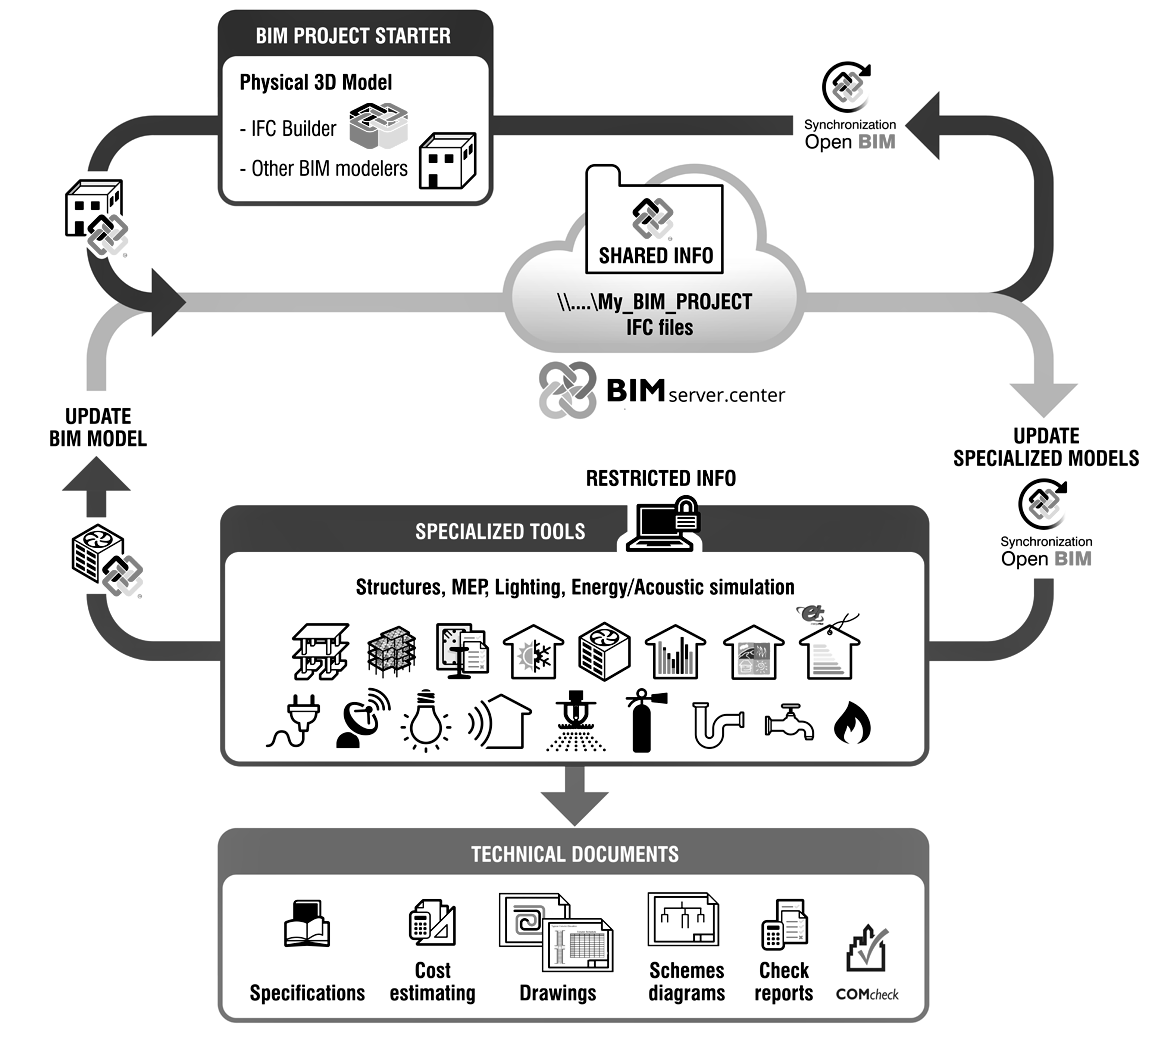
\includegraphics[width=0.5\textheight]{6_2_cap/img/cypeflow}
	\caption[Schema della filosofia BIM per CYPE]{Schema riassuntivo del funzionamento\\ della \emph{suite} CYPE con filosofia BIM.}
	\label{bim:cype}
\end{figure}

Per quanto riguarda la parte idronica si è utilizzato un applicativo BIM della software-house \emph{C.A.T.S.} che si appoggia ad \emph{Autodesk Autocad}.

È stato possibile definire inizialmente la tipologia di tubazioni da utilizzare (dimensioni, materiale e coibente), la metodologia di dimensionamento con le velocità minime ammissibili e poi disegnare direttamente in Autocad le tubazioni stesse posizionando le unità locali (radiatori e fancoil). Infine, l'applicativo ha dimensionato le tubazioni, rilasciato il computo metrico e la relazione di calcolo.
	\chapter{Lo stato attuale}
\thispagestyle{empty}
\section{Le modifiche al giorno d'oggi}
%Parla anche dell'assenza di organi per la misurazione dei consumi (elettrici e termici) e quindi problemi per la valutazione energetica \emph{ante-operam} e per il rispetto ai requisiti \emph{CAM}.\vspace{1em}
Nel primo capitolo si sono descritti in maniera sommaria l'architettura, l'edilizia e gli impianti presenti nell'intero complesso ospedaliero (al momento della costruzione) riportando le parole dell'\tit{ing.}{Corrado Beguinot}. 

In questo capitolo, invece, si vuole dare ampio spazio alle condizioni attuali del policlinico e dell'edificio stesso, riportando i dati di input inseriti all'interno dello studio pre-riqualificazione energetica e riferiti, quindi, allo stato di fatto. 

Riferendosi alla sola centrale termica del policlinico, nel marzo del 2004 è entrato in servizio il gruppo di cogenerazione a gas metano della potenza elettrica di \n{5.5}{MW} e \n{9}{MW} di potenza termica con caldaia a recupero. Il gruppo è costituito da:
\begin{itemize}
	\item una turbina \emph{Solar Turbines} modello \emph{Taurus T60};
	\item un produttore di energia elettrica \emph{Le Roy Somer -- Emerson};
	\item una caldaia a vapore \emph{Ruths}.	
\end{itemize}
I primi due sistemi (turbina e alternatore) sono assemblati in un unico package di produzione \emph{Turbomach} con in coda la caldaia a recupero.

La centrale è corredata anche da:
\begin{itemize}
	\item \num{4} assorbitori di vapore per produzione acqua refrigerata della potenza di \n{2691}{kW} cadauno \emph{ABTF750 -- Trane};
	\item \num{1} gruppo di assorbimento \emph{McQuay} da \n{4301}{kW};
	\item \num{2} caldaie \emph{Biasi} da \n{12}{MW} cadauna da utilizzarsi sporadicamente per integrazioni (nei periodi invernali con climi rigidi) e/o sostituzione della caldaia a recupero (in caso di manutenzione/guasto del gruppo di cogenerazione).
\end{itemize}

L'acqua surriscaldata viene prodotta a \n{130}{\degreeCelsius} e non più a \n{170}{\degreeCelsius} come avveniva in passato. I reflui termici alimentano da un lato la rete di teleriscaldamento e dall'altra il gruppo di assorbitori bistadio che a loro volta servono la rete di teleraffrescamento. Dei \num{4} assorbitori uno è di back-up. Un'altra modifica che ha interessato la centrale termica è stata la sostituzione delle torri evaporative giustificata da costi di manutenzione eccessivi nonché da un'evidente usura della struttura portante in legno. 

Per quanto riguarda la stagione estiva, invece, i gruppi ad assorbimento non risultano essere in grado, nonostante la recente installazione delle nuove macchine, di coprire il fabbisogno \emph{freddo} di tutto il policlinico a causa della diffusione dei fancoil e delle batterie di raffreddamento delle UTA (più numerose oggi che in passato). E se il gruppo ad assorbimento risulta essere \emph{sottodimensionato} ai carichi presenti oggigiorno nel policlinico, vi sono comunque i reflui termici del cogeneratore/caldaia che in estate non vengono utilizzati: si perde in ambiente una grande fonte di energia ad elevata temperatura. Nell'attesa di una riqualificazione dei vari edifici a cui sarebbe seguito senz'altro il montaggio dei fancoil, molti dipartimenti si sono autogestiti utilizzando \emph{split} per migliorare le condizioni termoigrometriche dei locali nella stagione estiva. Questo ha comportato un aumento di consumo di energia elettrica in tutto il policlinico.

\section{L'edificio 2}
Tutto il corpo di fabbrica è destinato alla \emph{Cardiochirurgia}.
\begin{figure}[t]
	\centering
	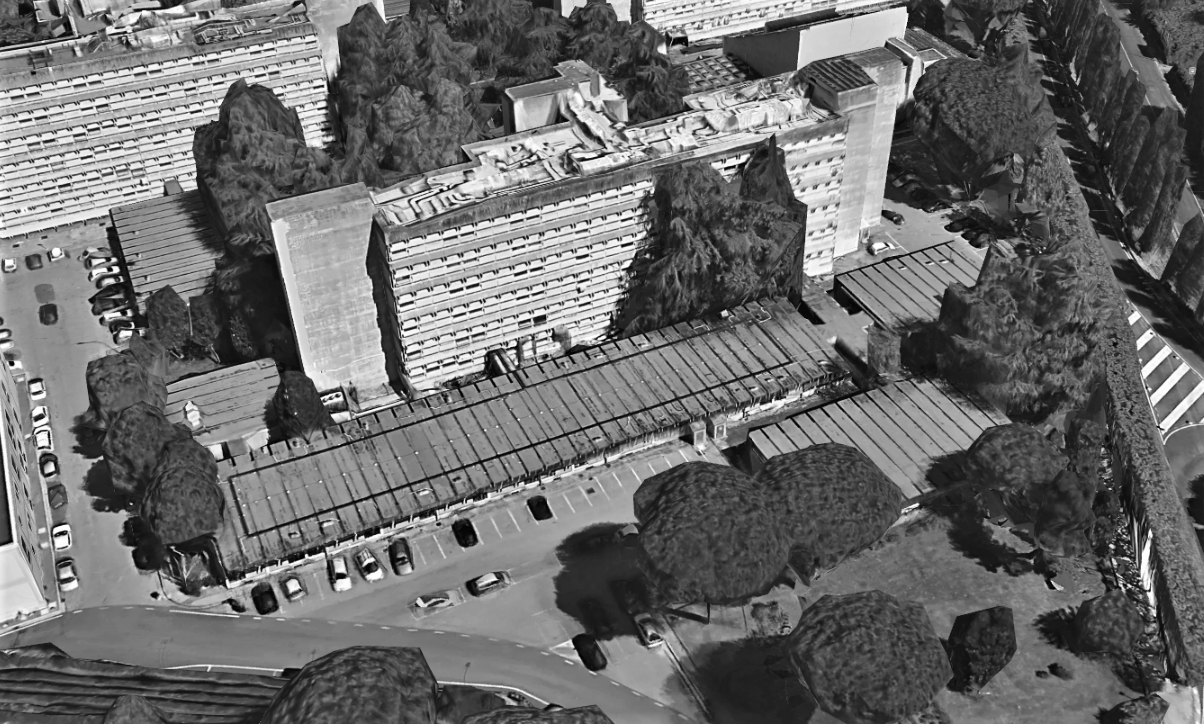
\includegraphics[width=\textwidth]{6_2_cap/img/SatellitareED2}
	\caption[Veduta satellitare dell'edificio 2 e dei suoi 5 corpi]{Veduta satellitare dell'edificio 2 e dei suoi 5 corpi. Fonte: \emph{Google Earth}.}
\end{figure}

Esso è costituito da 5 edifici:
\begin{itemize}
	\item Corpo A: è l'edificio principale. Di sviluppo longitudinale lungo un asse orientato lungo la direttrice NE--SO, è costituito da 6 piani fuori terra. Contiene le degenze, gli ambulatori, l'Emodinamica al piano terra, l'UTIC (Unità di Terapia Intensiva Coronarica) al primo piano e il blocco operatorio con terapia intensiva al quinto piano. La sua superficie coperta è di \n{5610}{m^2}, per singolo piano è di \n{935}{m^2} e un volume di circa \n{18700}{m^3};
	\item Corpo B: contiene gli stabulari. Di pianta pressoché quadrata (\n{102}{m^2}) è alto solo 1 piano; 
	\item Corpo C: contiene laboratori e ambulatori. E' di pianta rettangolare e alto solo 1 piano. Estensione di \n{812}{m^2};
	\item Corpo D: contiene ambulatori, studi medici e laboratori. Di pianta quadrata (\n{217}{m^2}) è alto solo 1 piano; 
	\item Corpo E: contiene ambulatori cardiologici, geriatrici e di medicina interna, vari laboratori e studi medici. È alto solo 1 piano con un'estensione di \n{305}{m^2}.
\end{itemize}

L'edificio 2 preserva tutte le opere edili e alcune impiantistiche realizzate all'epoca della sua costruzione. Non è difficile dedurre, quindi, che allo stato attuale sia i comportamenti estivi e invernali dell'involucro come le efficienze termo-meccaniche dell'impianto idro-aeraulico siano quantomeno inferiori a quelli consigliati dalla norma attuale vigente. In \vref{pan} è presente una panoramica in cui è possibile apprezzare i vari corpi. In \vref{IFC} sono state riportate \num{3} immagini del modello tridimensionale dell'edificio 2 costruito con \textbf{IFC Builder}. Il file è stato poi importato nel \textbf{LOAD} da cui sono stati estratti i carichi termici. È interessante notare la verosimiglianza delle suddette immagini con quelle reali riportate in \vref{ed21} e \ref{ed22}.

L'analisi progettuale ha come oggetti di intervento il corpo A e C. In particolare, del primo non si interessa nel quinto piano (dove è situato il blocco operatorio) e degli impianto dell'UTIC e dell'Emodinamica.

Riassumendo: il corpo A verrà riqualificato \emph{civilmente} in tutti i piani escluso il quinto piano e i tre pozzi delle scale; l'intervento impiantistico interesserà, invece, tutto il corpo A esclusi i tre pozzi delle scale, l'UTIC, l'Emodinamica e tutto il quinto piano; il corpo C verrà riqualificato integralmente sia \emph{civilmente} che \emph{impiantisticamente}. 

Da ciò discende la necessità di modellare termo-fisicamente le sole zone oggetto dell'intervento. Paradossalmente, però, per dimensionare l'impianto della sottocentrale si è tenuto conto anche, ovviamente, del quinto piano in quanto ad esso si appoggia.

\begin{figure}
	\centering
	\subfloat[][Facciata meridionale]{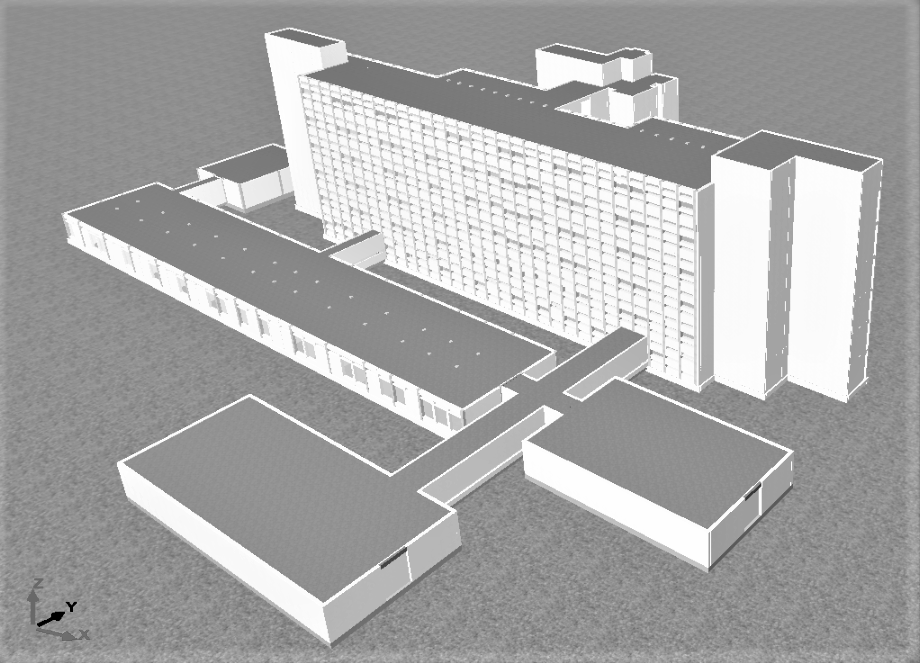
\includegraphics[width=0.6\textwidth]{6_2_cap/img/IFC1}\label{ifc1}}\\
	\subfloat[][Facciata settentrionale]{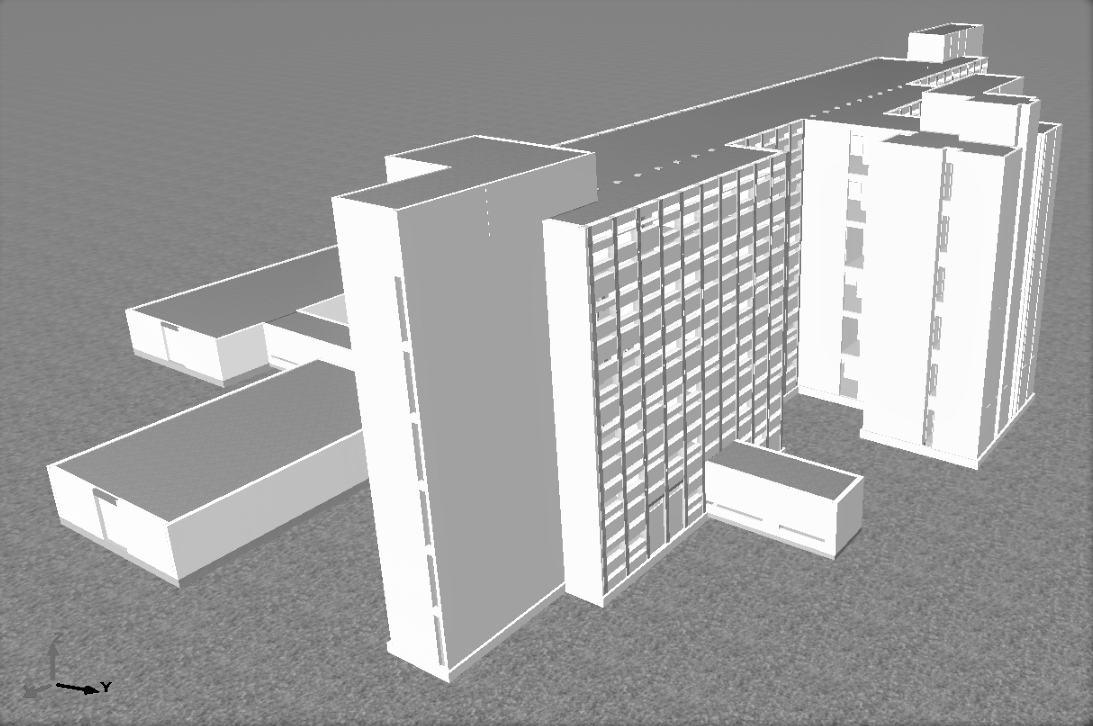
\includegraphics[width=0.6\textwidth]{6_2_cap/img/IFC2}\label{ifc2}}\\
	\subfloat[][Facciata settentrionale]{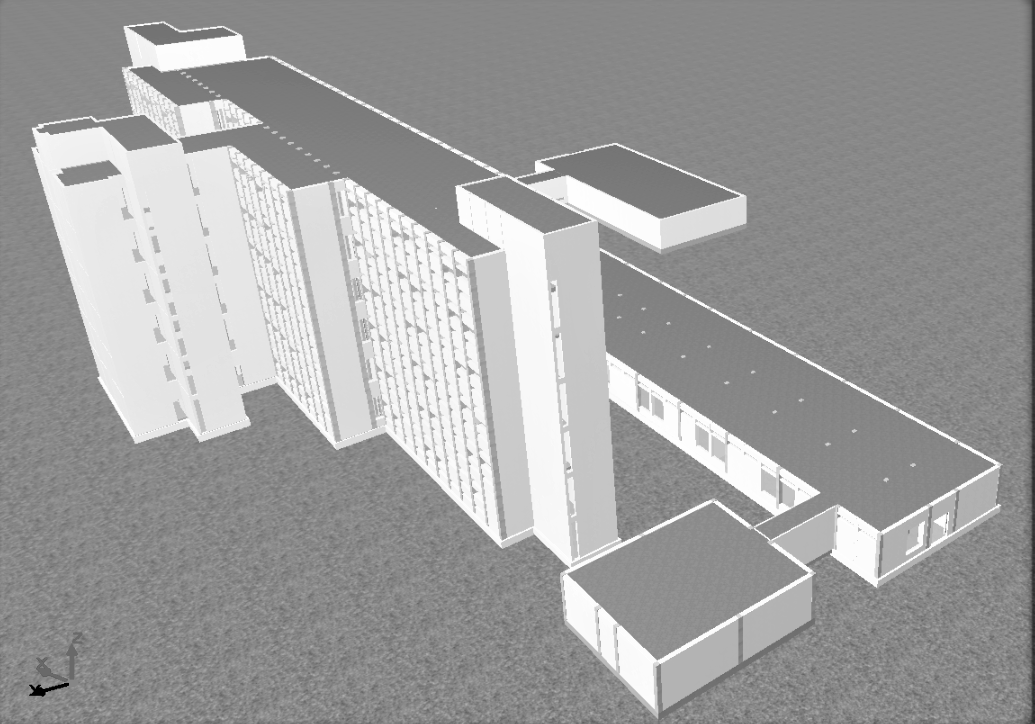
\includegraphics[width=0.6\textwidth]{6_2_cap/img/IFC3}\label{ifc3}}
	\caption{Modelli tridimensionali dell'edificio 2.}\label{IFC}
\end{figure}

\begin{sidewaysfigure}
	\centering
	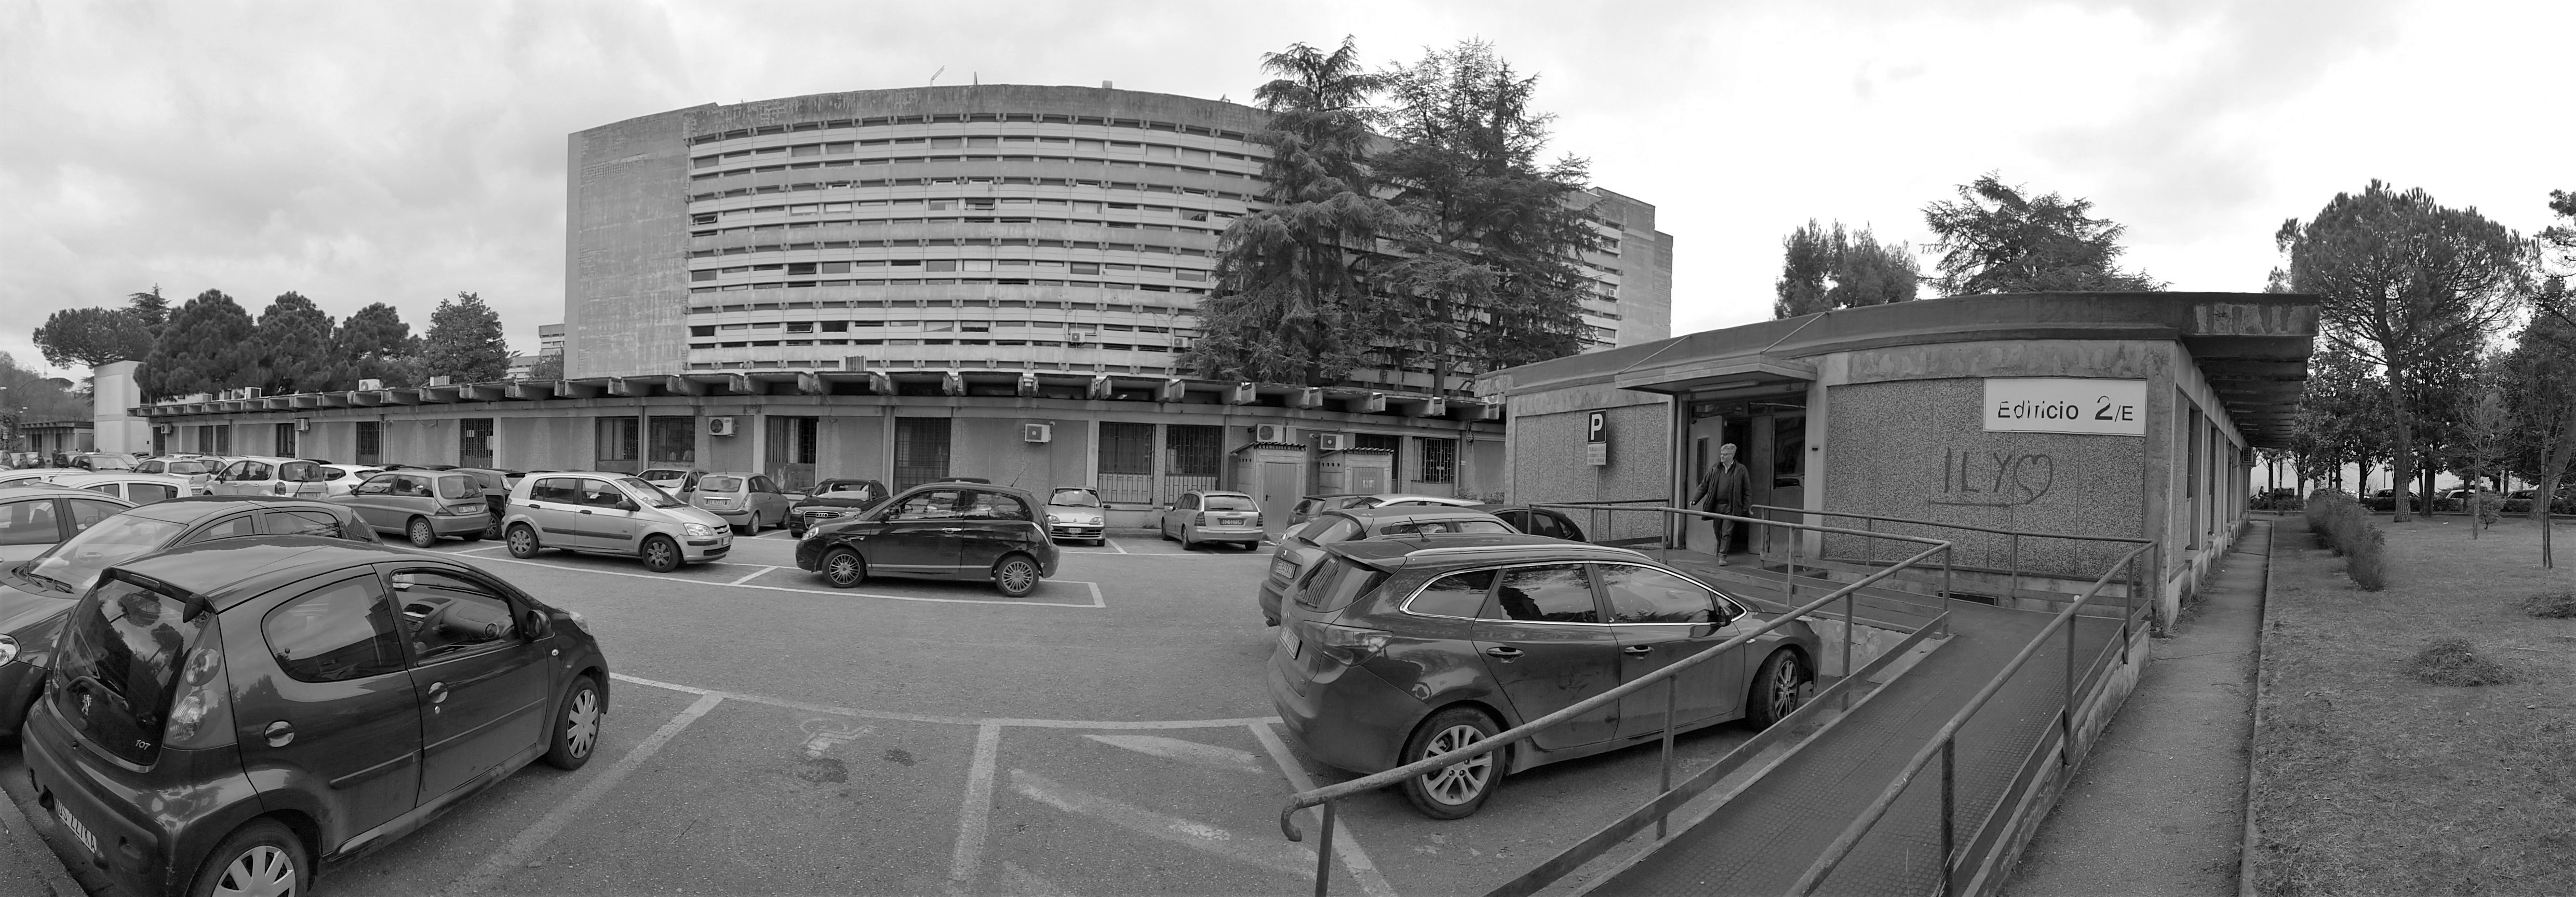
\includegraphics[scale=0.11]{6_2_cap/img/pan}
	\caption[Panoramica dell'edificio 2.]{Panoramica dell'edificio 2: a destra il corpo E; al centro il corpo C e in fondo in alto il corpo A. È possibile apprezzare il gioco di pieni e vuoti dei blocchi di silicalcite e finestre.}\label{pan}
\end{sidewaysfigure}

\clearpage
\section{L'involucro}
L'involucro dell'Edificio 2, sia quello opaco che quello trasparente, non è cambiato in questi anni quindi non ci sono differenze con le stratigrafie indicate dall'\tit{Ing.}{Corrado Beguinot}.

Prima di descrivere come sono stati modellati i vari componenti opachi, è doveroso sottolineare la presenza notevole di ponti termici geometrici e materiali che aumentano il carico invernale e estivo.

\begin{figure}
	\centering
	\subfloat[][\emph{Facciata meridionale del Corpo A.}]{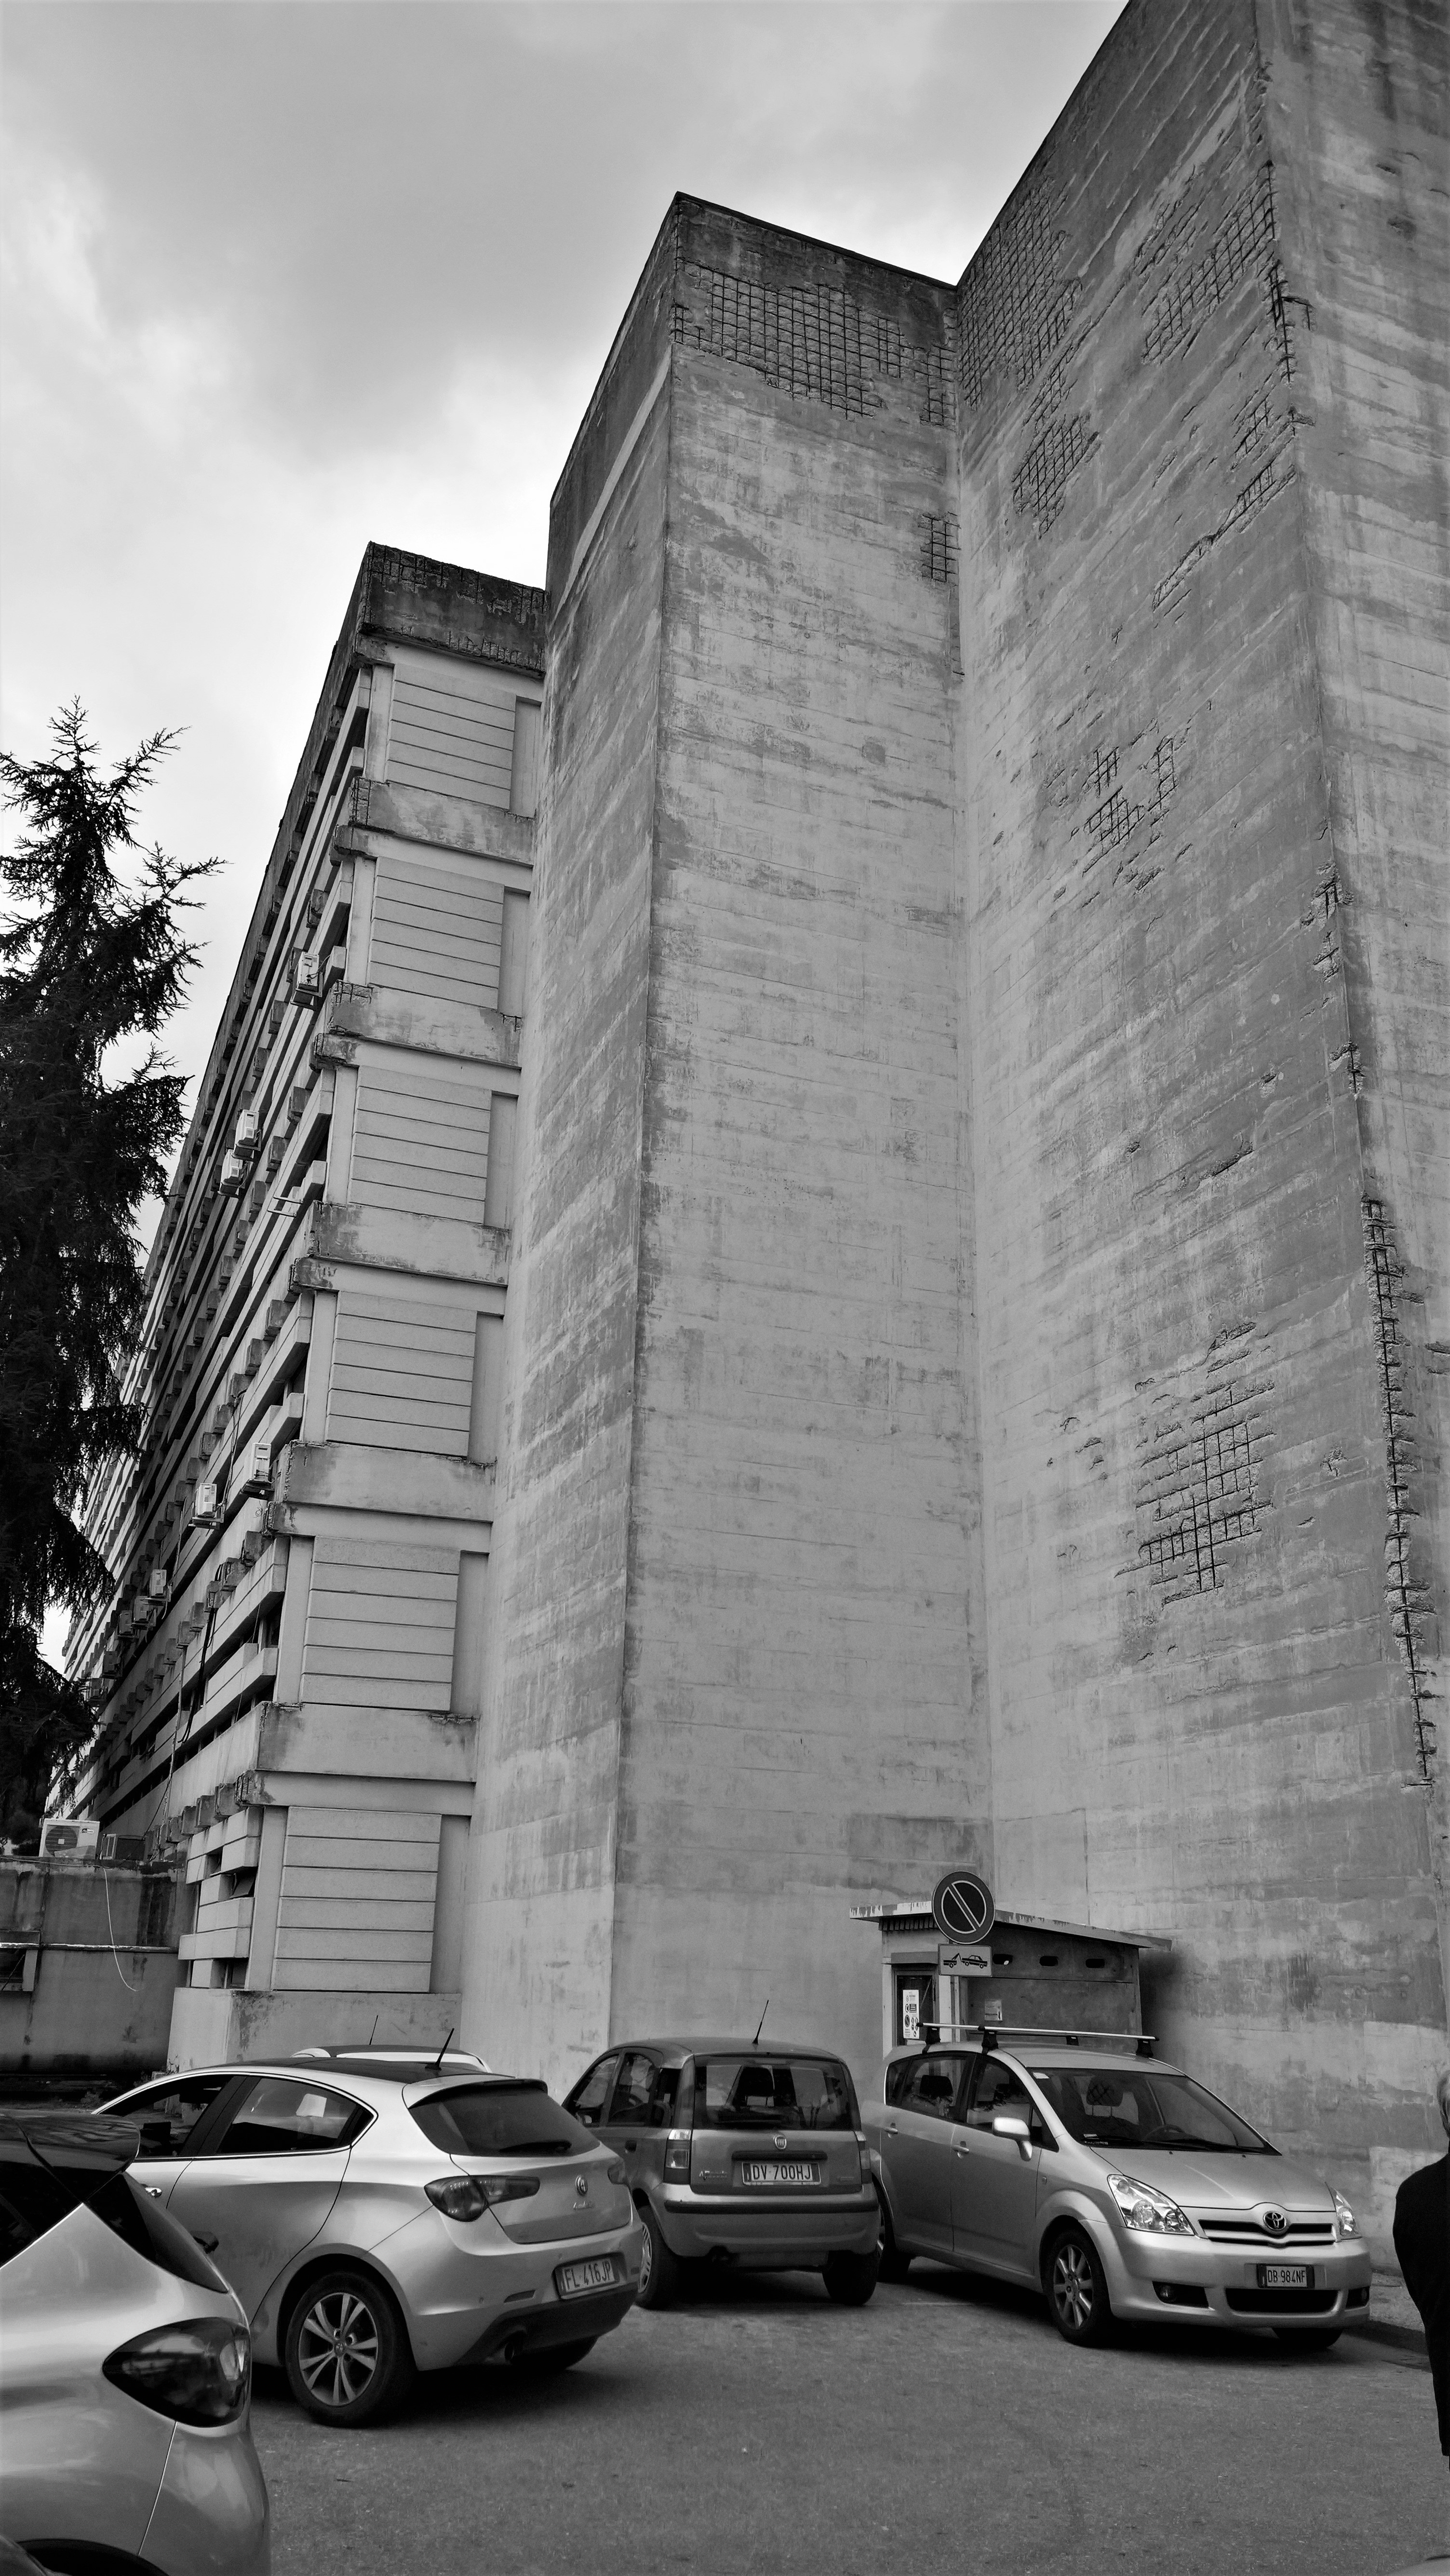
\includegraphics[height=0.4\textheight]{6_2_cap/img/ed2dx}\label{ed21}}\quad
	\subfloat[][\emph{Facciata settentrionale del Corpo A. Qui è presente l'ingresso per il pubblico.}]{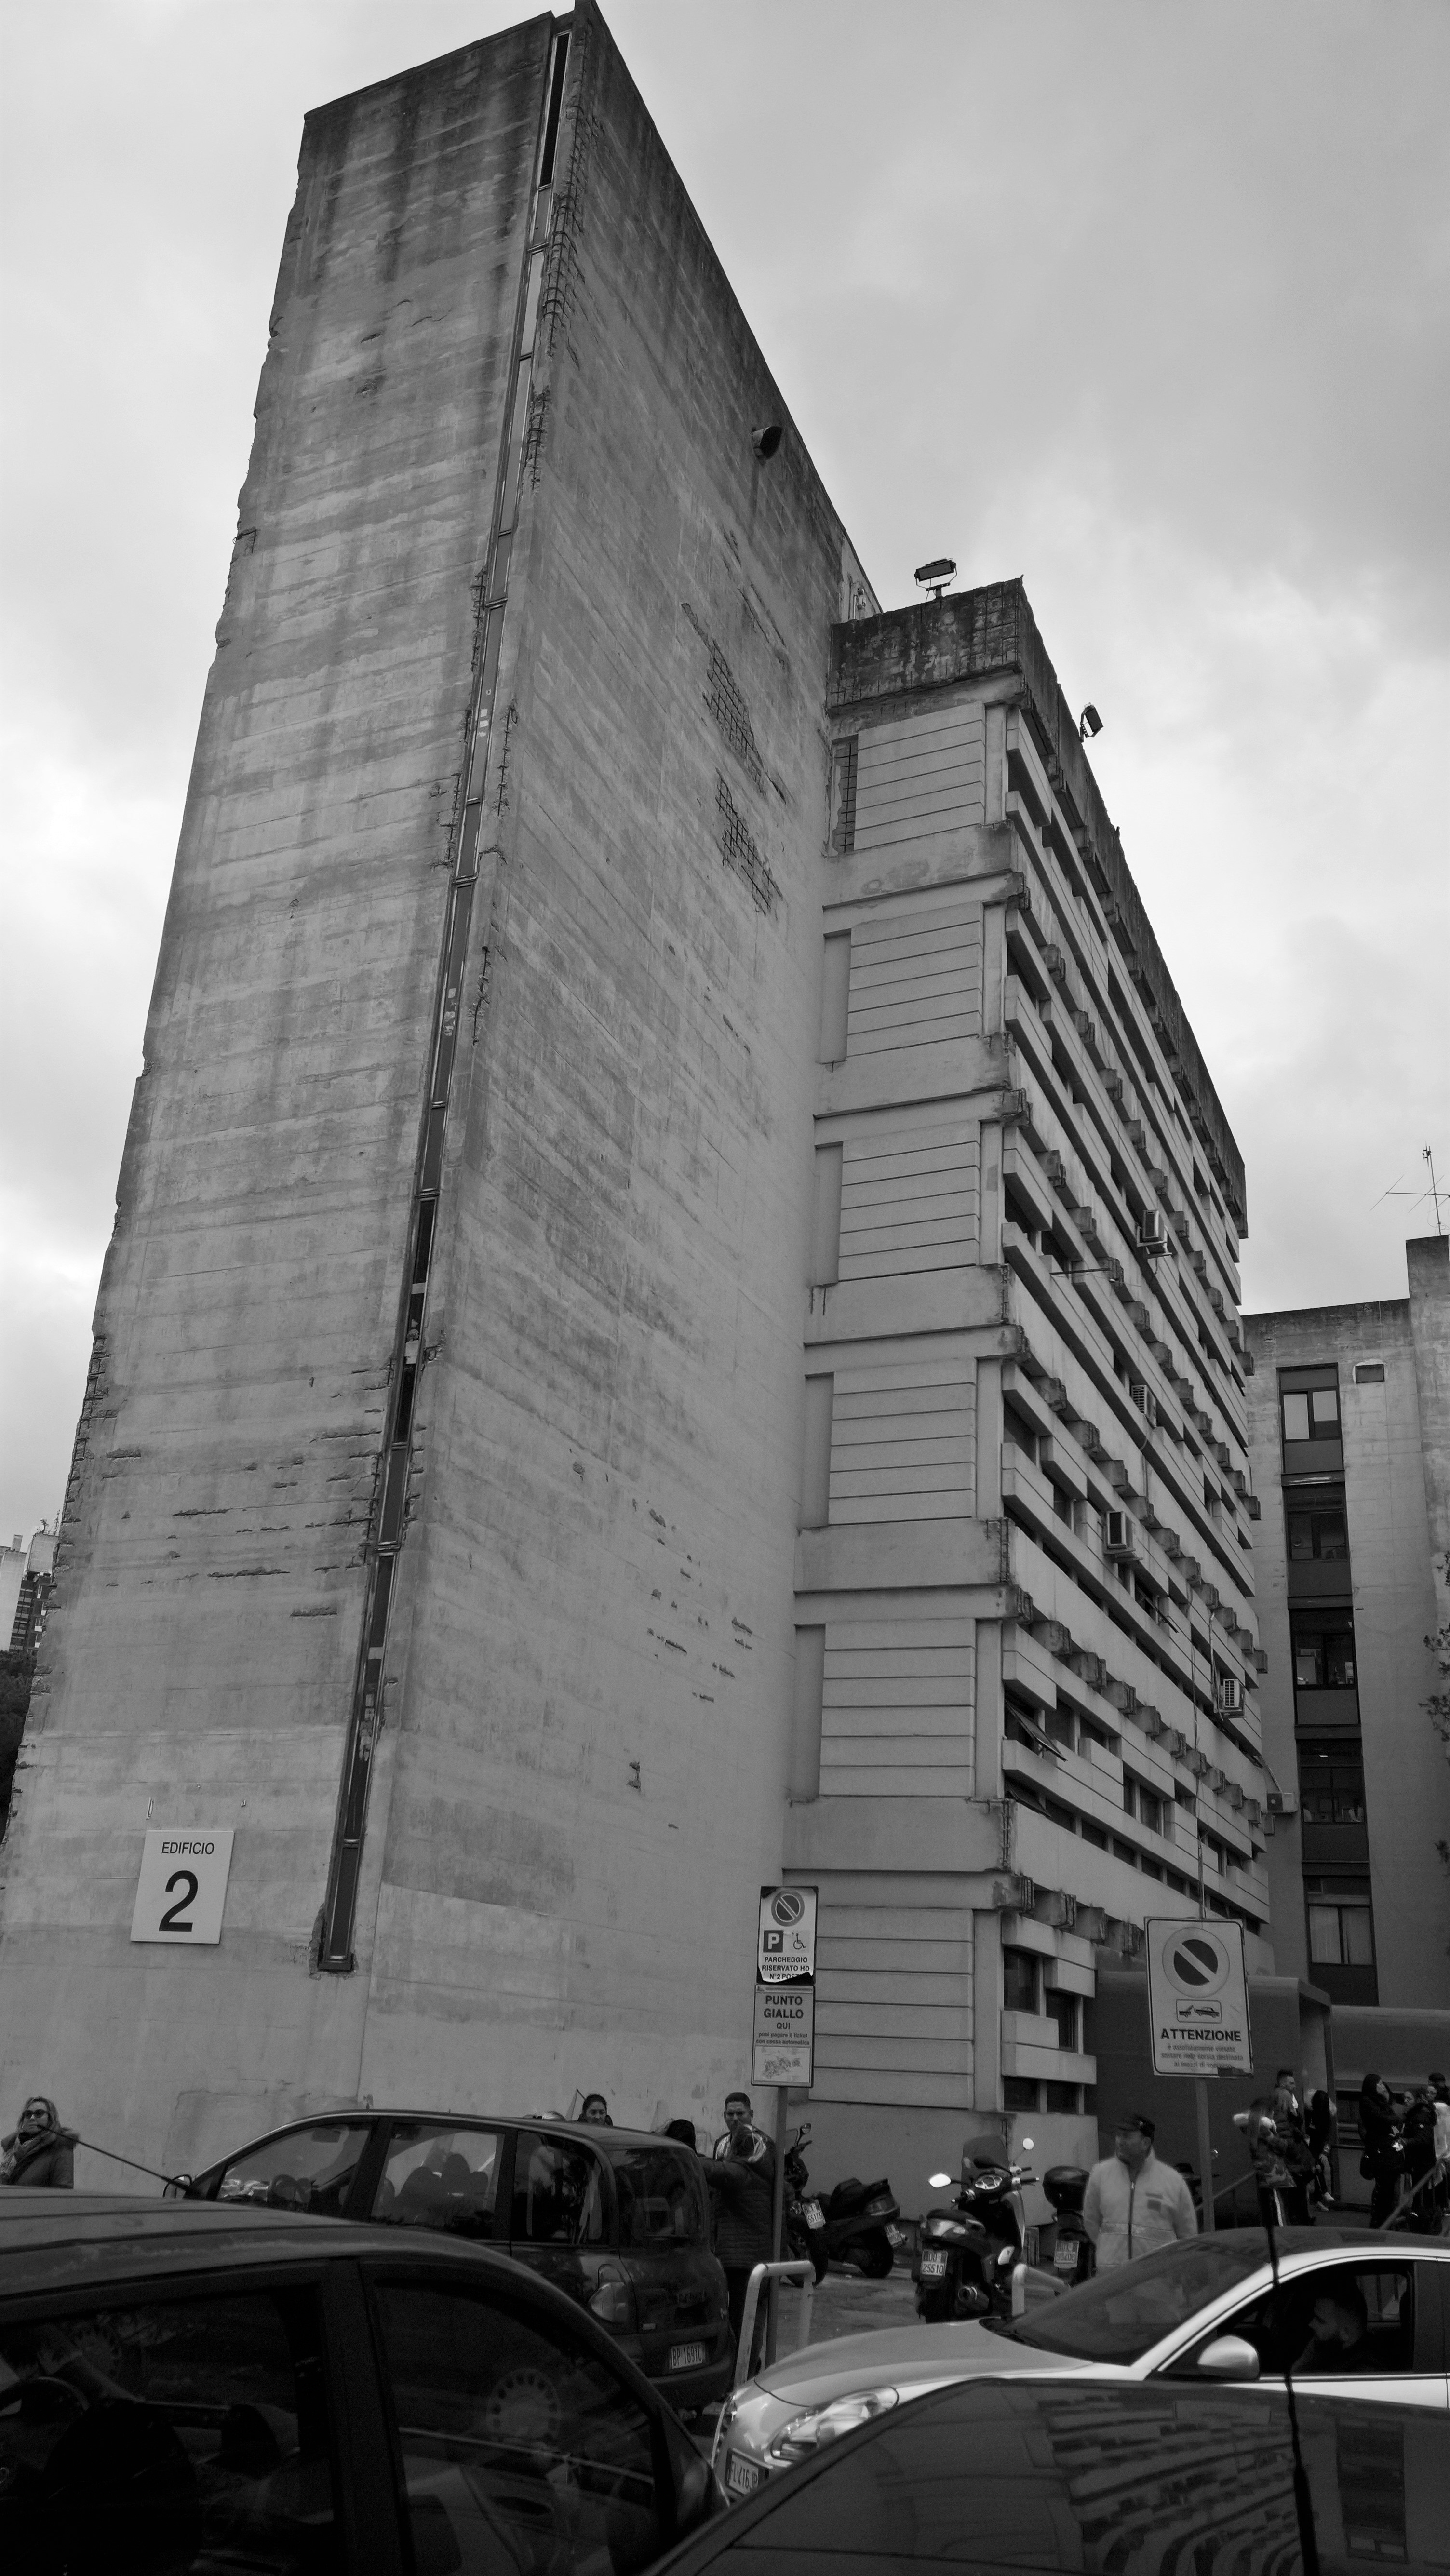
\includegraphics[height=0.4\textheight]{6_2_cap/img/ed2sx}\label{ed22}}	\\
	\subfloat[][\emph{Particolare dei blocchi di silicalcite.}]{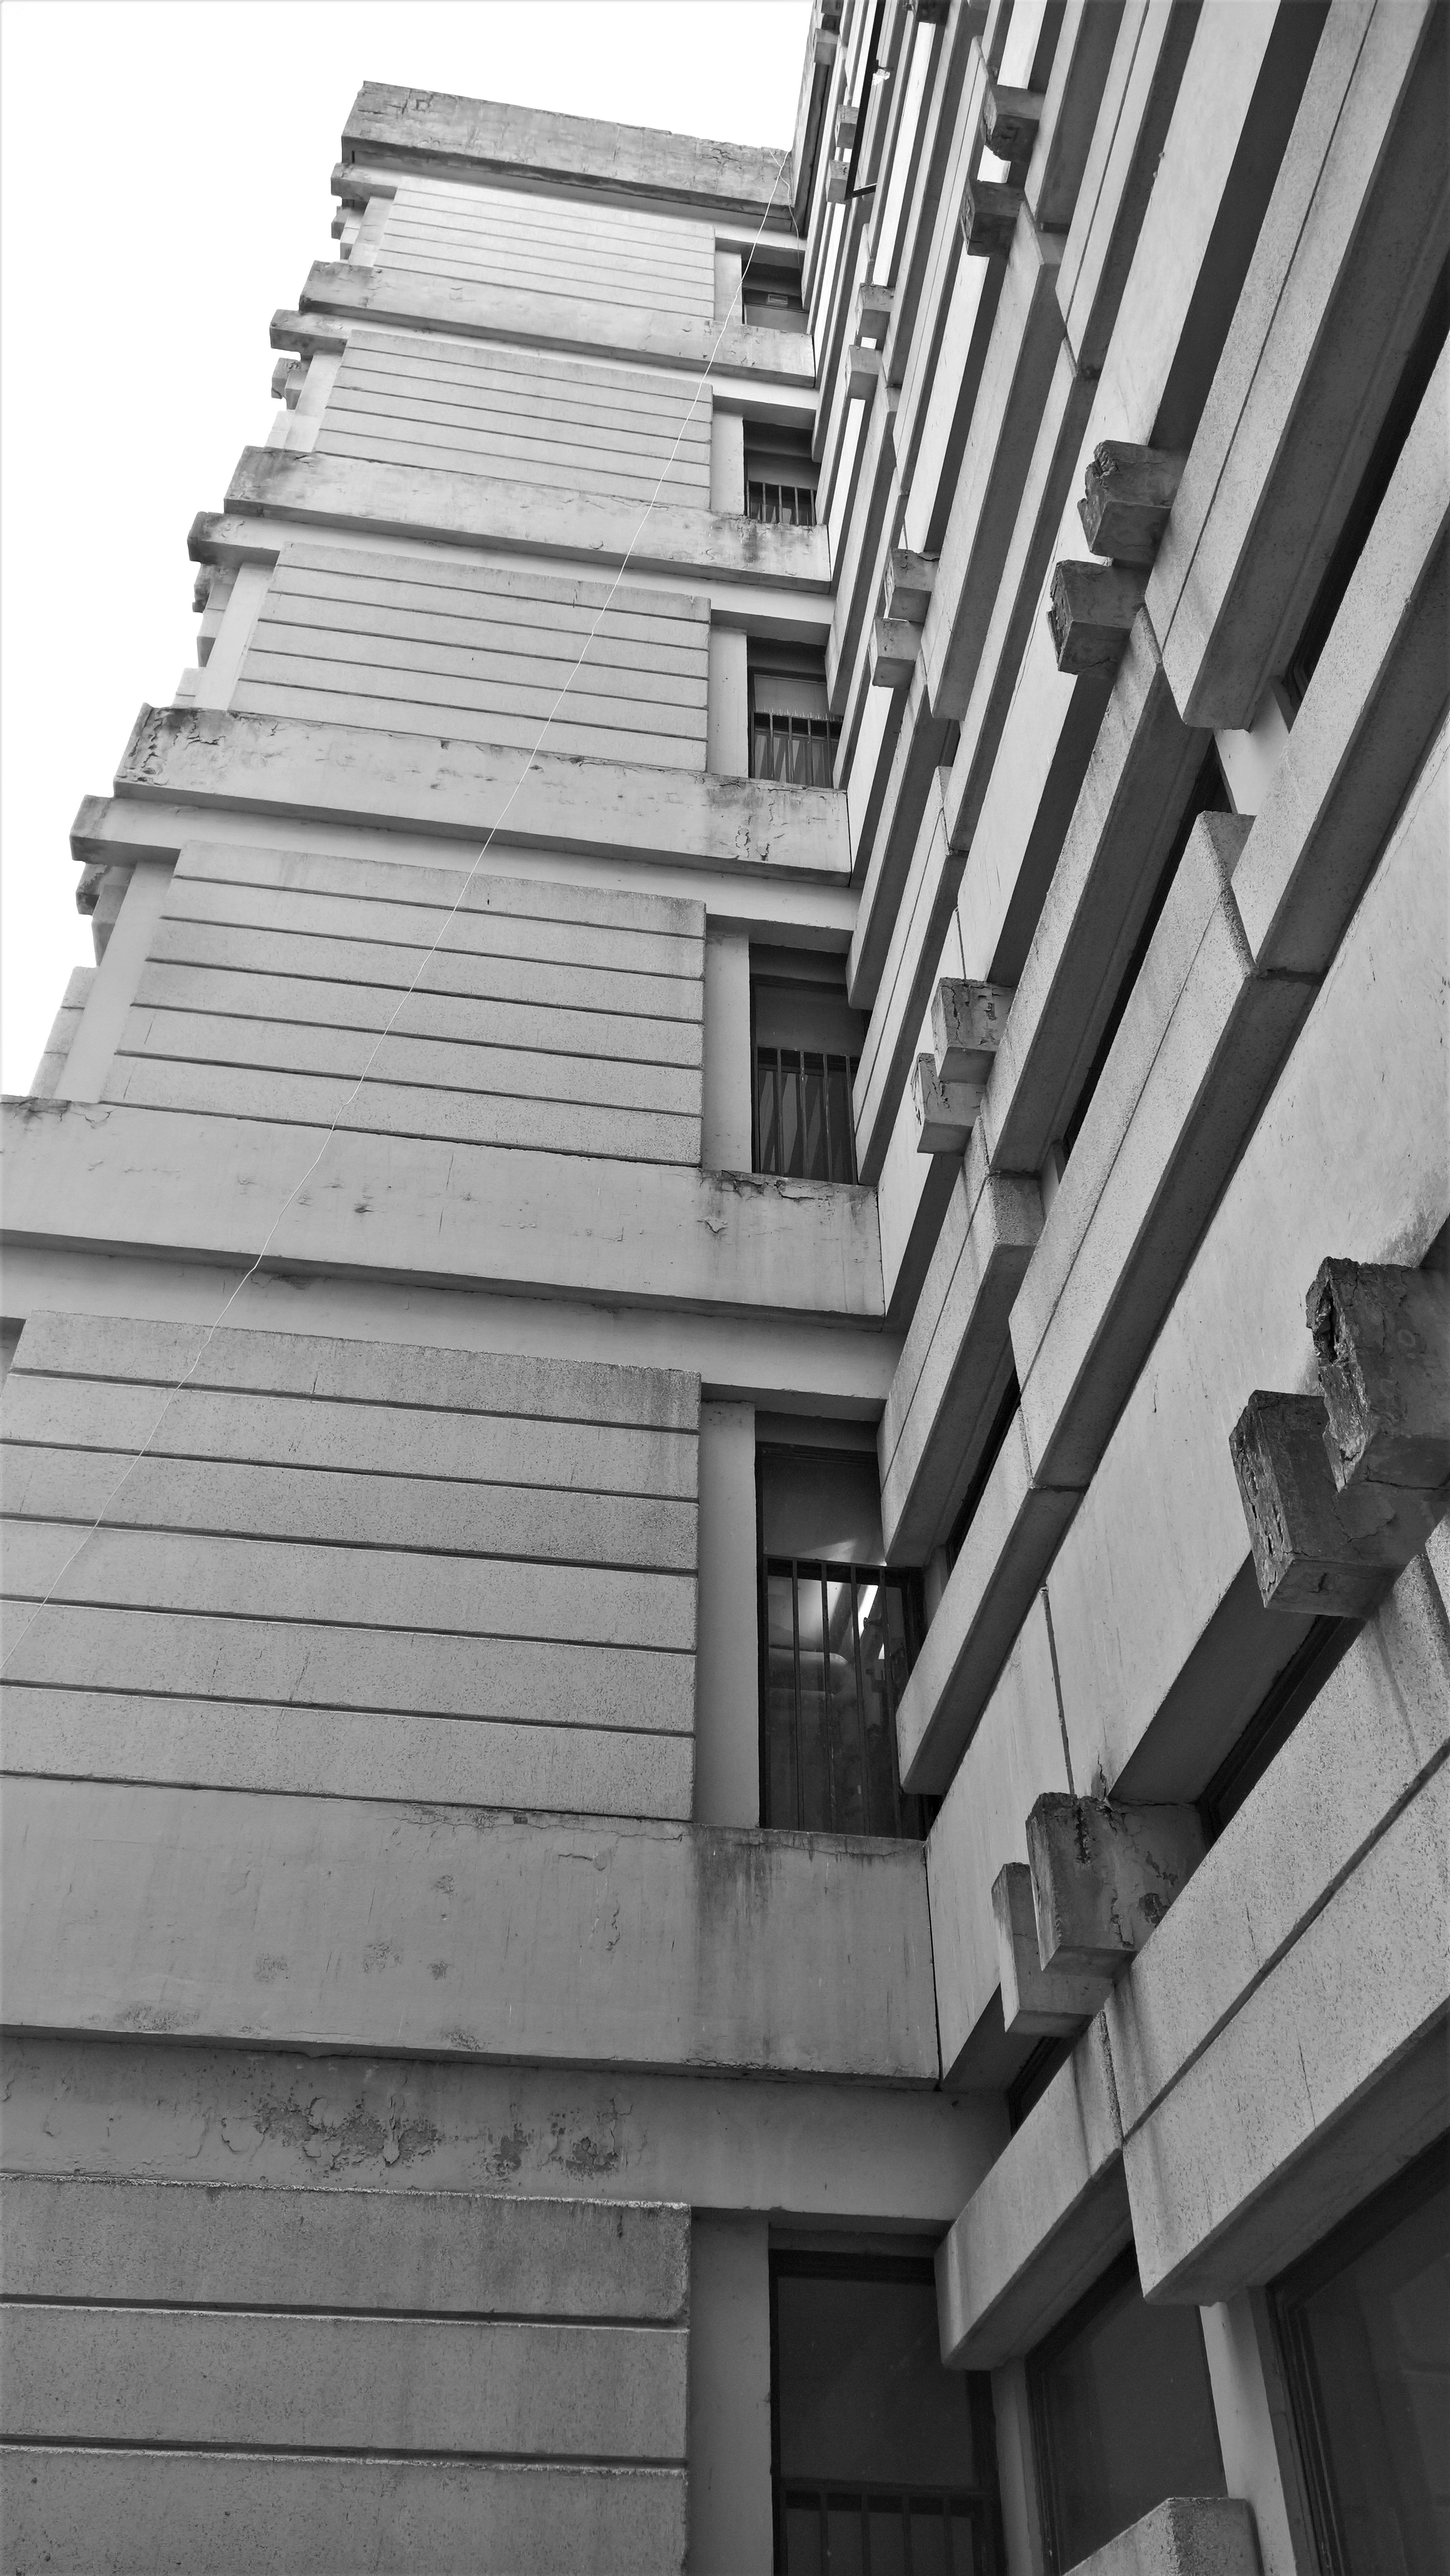
\includegraphics[height=0.4\textheight]{6_2_cap/img/ed23}} \quad
	\subfloat[][\emph{Ingresso secondario privato.}]{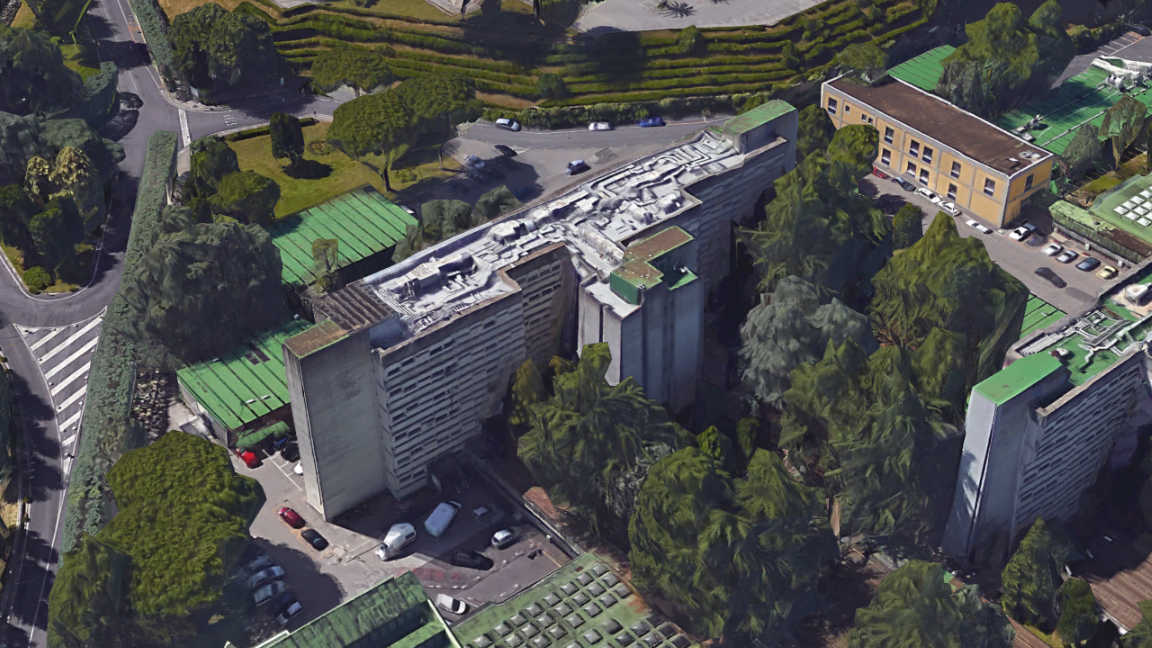
\includegraphics[height=0.4\textheight]{6_2_cap/img/ed22}}
	\caption{L'edificio 2. Particolari del Corpo A.}\label{esterno}
\end{figure}

Segue, quindi, la descrizione numerica dei componenti (opachi e trasparenti) utilizzati come dati di input per il calcolo del fabbisogno energetico e del carico termico (estivo e invernale) dell'edificio stesso.
\subsection{Componenti opachi}
\subsubsection{MURO EXT}
È il componente esterno verticale delle facciate maggiori del Corpo A. \\È caratterizzato esternamente da blocchi di silicalcite alternati dagli infissi. \\Questa tipologia di muro è fittizia poiché si è modellato un componente che nella realtà è caratterizzata da una diversa stratigrafia in senso verticale. Dal punto di vista numerico, quindi, si è effettuata una media ponderale delle varie caratteristiche termo-fisiche in modo tale che il risultato finale sia quanto più possibile veritiero. La parte inferiore è costituita semplicemente da un mattone forato da \n{10}{cm} intonacato internamente ed esternamente; la parte superiore, invece, è caratterizzata dai blocchi di silicalcite. \\ La stratigrafia della parte superiore è (dall'interno verso l'esterno):
\begin{center}
	\begin{tabular}{lcc}
		\toprule
		Componente & Spessore [m] & Conduttività [\si{W/mK}] \\
		\midrule
		Acciao & \num{0.01} & \num{50.0} \\
		Intercapedine d'aria & \num{0.05} & -\\
		CLS & \num{0.35} & \num{1.06} \\
		\bottomrule
	\end{tabular}
\end{center}
Questi i risultati del componente modellato (a valle della media ponderale):
\begin{center}
	\begin{tabular}{lcc}
		\toprule
		Spessore & \num{0.43} & \si{m}\\
		Trasmittanza & \num{1.423} & \trasm\\
		Trasmittanza termica periodica & \num{0.190} & \trasm\\
		\bottomrule
	\end{tabular}
\end{center}
\newpage
\subsubsection{MURO EXT 200}
È il componente esterno delle pareti in cemento armato.
\begin{center}
	\begin{tabular}{lcc}
		\toprule
		Componente & Spessore [m] & Conduttività [\si{W/mK}] \\
		\midrule
		Malta di calce-cemento & \num{0.01} & \num{0.90} \\
		CLS & \num{0.18} & \num{1.48}\\
		Malta di calce-cemento & \num{0.01} & \num{0.90} \\
		\bottomrule
	\end{tabular}
\end{center}
Questi i risultati del componente modellato:
\begin{center}
	\begin{tabular}{lcc}
		\toprule
		Spessore & \num{0.20} & \si{m}\\
		Trasmittanza & \num{3.29} & \trasm\\
		Trasmittanza termica periodica & \num{1.71} & \trasm\\
		\bottomrule
	\end{tabular}
\end{center}

\subsubsection{MURO EXT Corpo Basso}
È il componente esterno verticale dei corpi bassi ovvero B, C, D ed E.
\begin{center}
	\begin{tabular}{lcc}
		\toprule
		Componente & Spessore [m] & Conduttività [\si{W/mK}] \\
		\midrule
		Malta di calce-cemento & \num{0.01} & \num{0.90} \\
		Mattone forato & \num{0.08} & -\\
		Intercapedine d'aria & \num{0.05} & - \\
		CLS & \num{0.1} & \num{1.91}\\
		\bottomrule
	\end{tabular}
\end{center}
Questi i risultati del componente modellato:
\begin{center}
	\begin{tabular}{lcc}
		\toprule
		Spessore & \num{0.24} & \si{m}\\
		Trasmittanza & \num{1.63} & \trasm\\
		Trasmittanza termica periodica & \num{1.06} & \trasm\\
		\bottomrule
	\end{tabular}
\end{center}
\subsubsection{COPERTURA 1}
È la copertura del Corpo A.\\Già oggetto di interventi passati, le sue caratteristiche termo-fisiche sono così riassunte:
\begin{center}
	\begin{tabular}{lcc}
		\toprule
		Spessore & \num{0.38} & \si{m}\\
		Trasmittanza & \num{0.36} & \trasm\\
		Trasmittanza termica periodica & \num{0.10} & \trasm\\
		\bottomrule
	\end{tabular}
\end{center}
\subsubsection{COPERTURA 2}
È la copertura dei Corpi B, C, D ed E. In \vref{cap2} si può apprezzare l'elevato stato di usura dei prefabbricati costituenti la copertura dei corpi \emph{bassi}.
\begin{figure}[h]
	\centering
	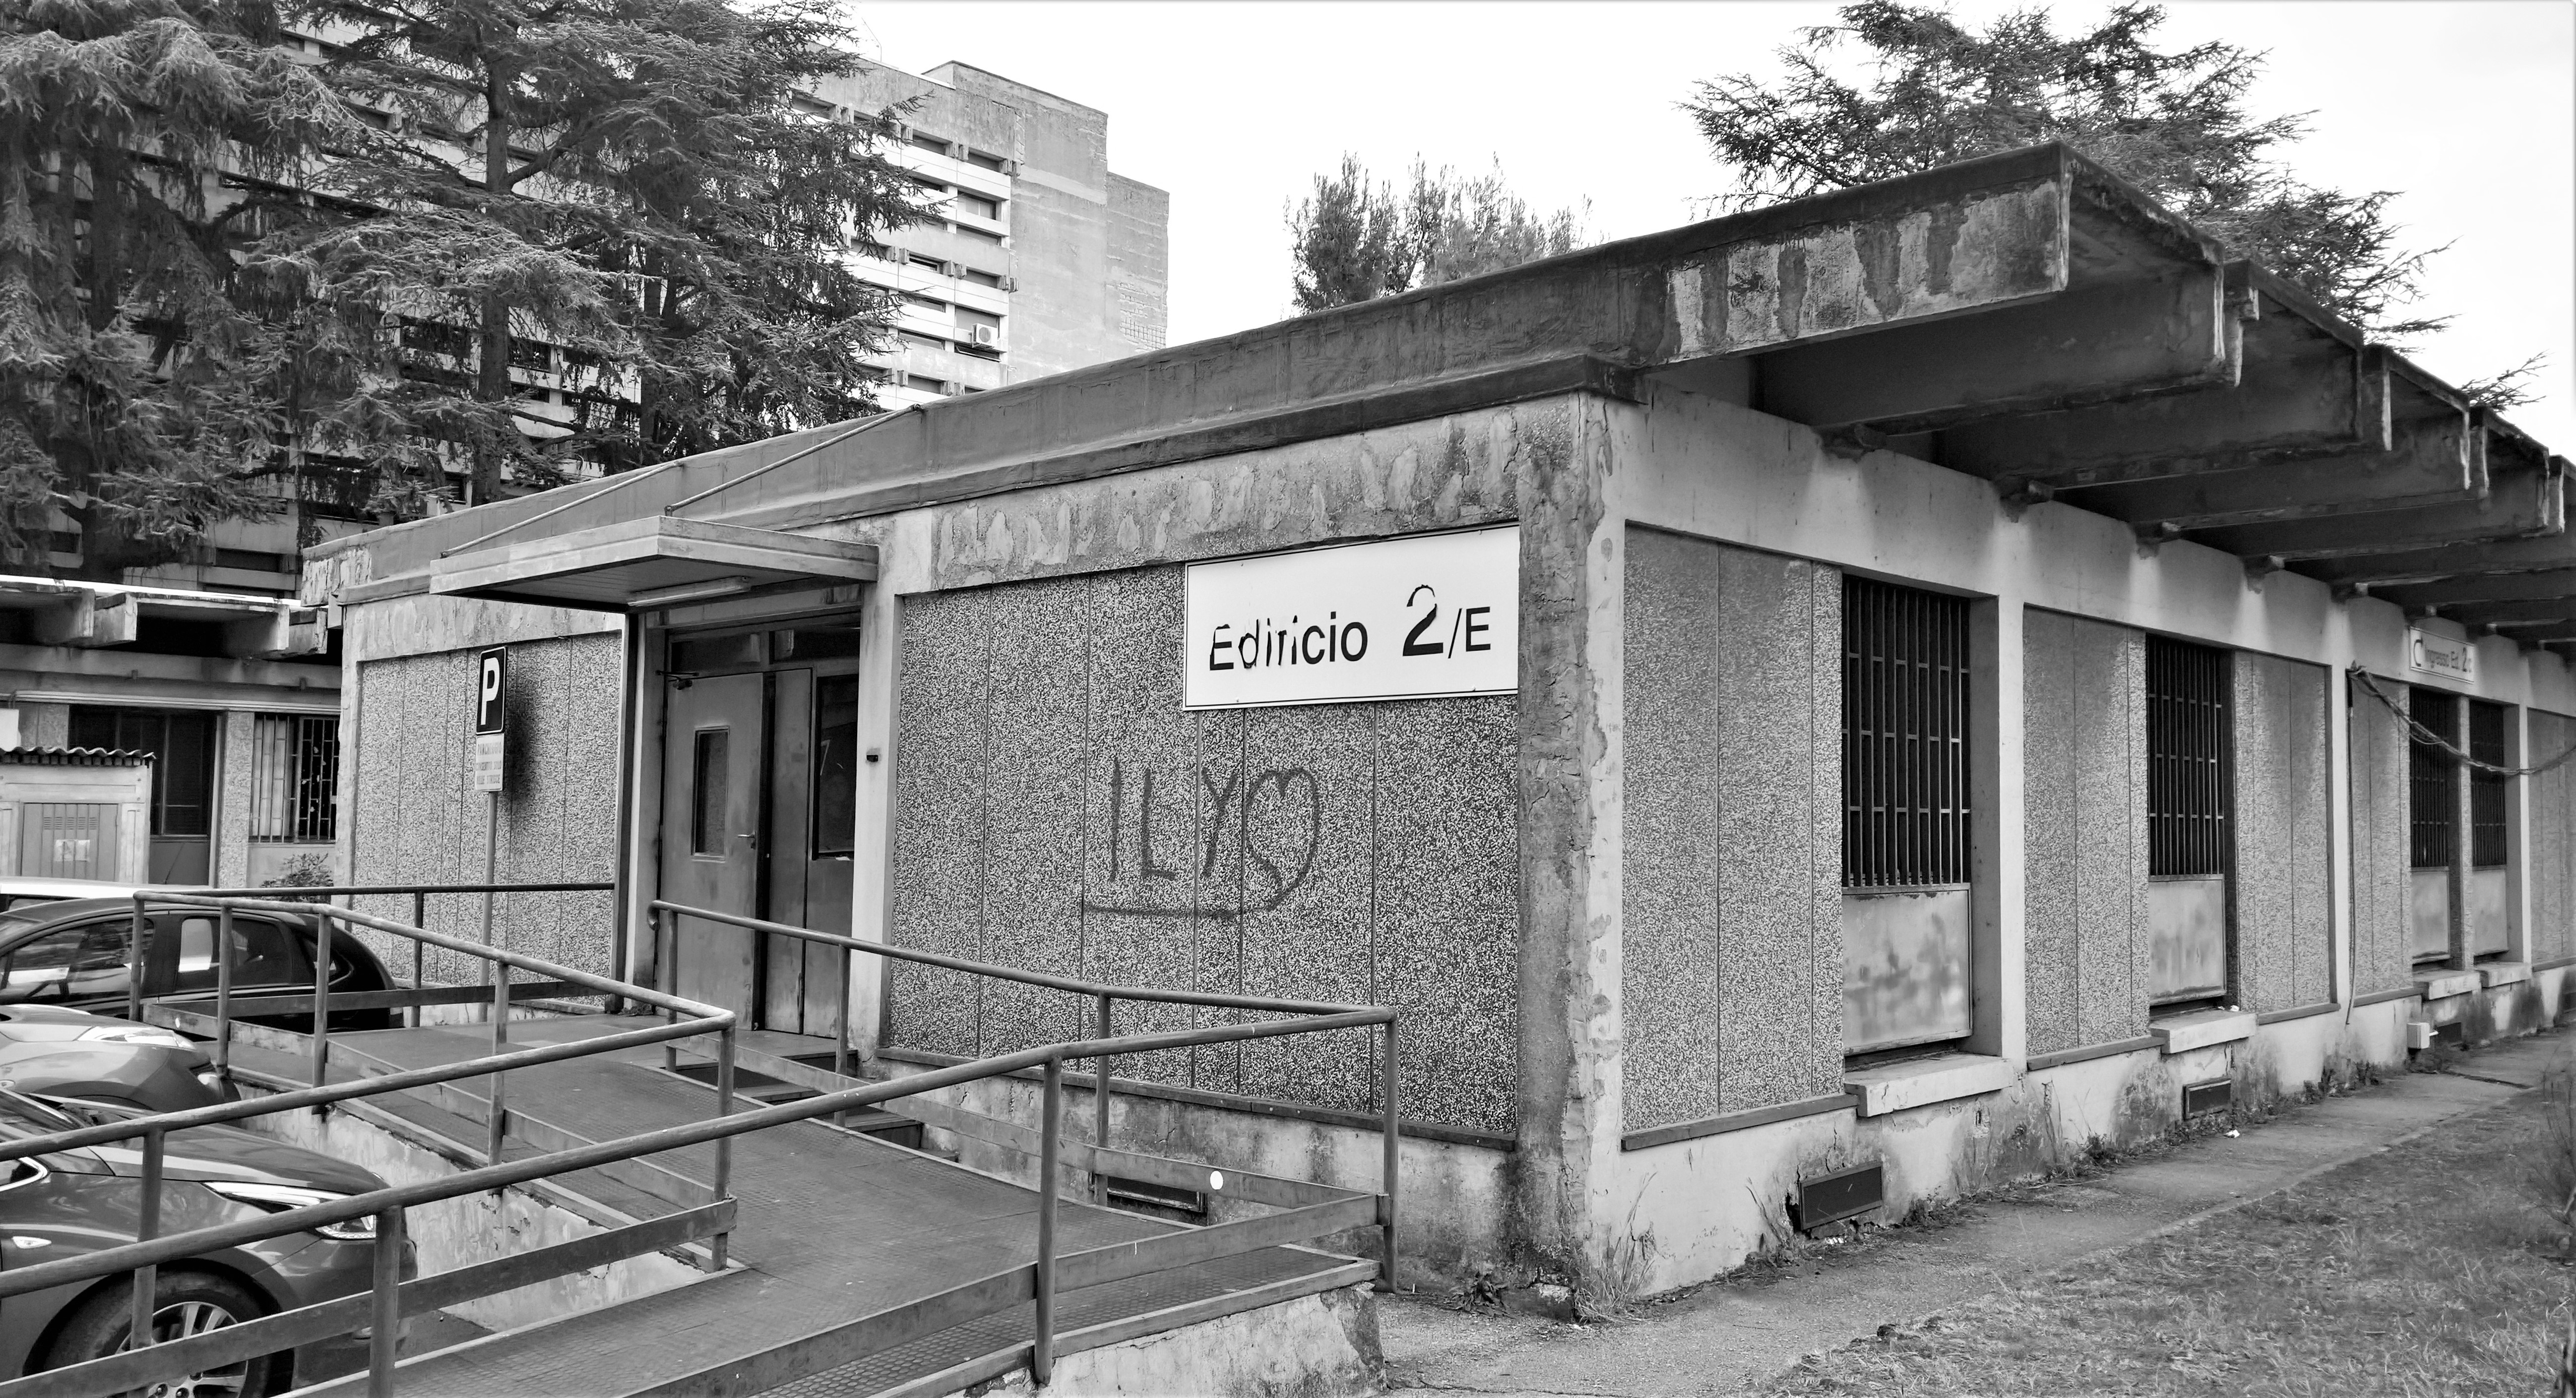
\includegraphics[width=\textwidth]{6_2_cap/img/cop2}
	\caption[Veduta esterna del corpo E]{Veduta esterna del corpo E. Sullo sfondo il corpo C e A.}\label{cap2}
\end{figure}
\begin{center}
	\begin{tabular}{lcc}
		\toprule
		Componente & Spessore [m] & Conduttività [\si{W/mK}] \\
		\midrule
		Intonaco di Calce e Gesso & \num{0.02} & \num{1.61} \\
		CLS SC  & \num{0.09} & \num{1.48}\\
		CLS SA & \num{0.10} & \num{0.58} \\
		Bitume su carta e cartone & \num{0.0050} & \num{0.23} \\
		\bottomrule
	\end{tabular}
\end{center}
Questi i risultati del componente modellato:
\begin{center}
	\begin{tabular}{lcc}
		\toprule
		Spessore & \num{0.22} & \si{m}\\
		Trasmittanza & \num{2.39} & \trasm\\
		Trasmittanza termica periodica & \num{1.07} & \trasm\\
		\bottomrule
	\end{tabular}
\end{center}
\newpage
\subsubsection{PAVIMENTO}
È il componente opaco utilizzato per modellare il pavimento dell'Edificio 2 (quindi in comune a tutti i corpi). È bene precisare che questo componente non è a contatto con il terreno in quanto vi sono i locali della sottocentrale nel piano -1.\\
Questi i risultati:
\begin{center}
	\begin{tabular}{lcc}
		\toprule
		Componente & Spessore [m] & Conduttività [\si{W/mK}] \\
		\midrule
		Piastrelle di Ceramica & \num{0.01} & \num{1.30} \\
		CLS SC & \num{0.08} & \num{1.61}\\
		Blocco da solaio & \num{0.22} & - \\
		\bottomrule
	\end{tabular}
\end{center}
\begin{center}
	\begin{tabular}{lcc}
		\toprule
		Spessore & \num{0.31} & \si{m}\\
		Trasmittanza & \num{1.38} & \trasm\\
		Trasmittanza termica periodica & \num{0.35} & \trasm\\
		\bottomrule
	\end{tabular}
\end{center}
\clearpage
\subsection{Componenti trasparenti}
Come è già stato ampiamente detto, tutti gli infissi risultano essere ancora quelli originali.

Per la loro modellazione sono stati usati gli stessi dati termo-fisici ($U_g$, $U_f$ e $U_w$) mentre sono stati differenziati solo geometricamente.
Il telaio è metallico senza taglio termico con un unico vetro (spessore di \n{4}{mm} senza alcun trattamento superficiale).

Questi i risultati:
\begin{center}
	\begin{tabular}{lcc}
		\toprule
		$U_g$ & \num{5.747} & \multirow{3}*{\trasm}\\
		$U_f$ & \num{5.800} &\\
		$U_g$ & \num{5.760} &\\
		\bottomrule
	\end{tabular}
\end{center}

Si elencano ora i vari infissi utilizzati all'interno del modello dell'edificio:
\begin{itemize}
	\item \textbf{PICCOLA} \n{1.60x0.33}{m}.\\ È il componente trasparente facente parte delle facciate maggiori del Corpo~A. 
	\item \textbf{GRANDE} \n{1.60x0.67}{m}.\\ È la variante alta della finestra \textbf{PICCOLA}. 
	\item \textbf{LUCERNARIO} \n{1.45x0.39}{m}.\\ Questo è il lucernario presente nella parte superiore di ogni modulo delle due facciate maggiori del Corpo A. In \vref{unitloca} si possono vedere queste 3 tipologie di componenti trasparenti che caratterizzano le facciate maggiori del corpo A.
	\item \textbf{QUADRA} \n{0.75x0.75}{m}. Vedere \vref{finq}.
	\item \textbf{LUNGA} \n{0.75x1.70}{m}.\\ Presente al di sotto della finestra \textbf{QUADRA}, insieme a quest'ultima crea un unico infisso che percorre tutta l'altezza del Corpo A nelle scanalature del muro \textbf{MURO EXT 200}. 
	\item \textbf{FIN-160} \n{1.60x3.00}{m}. \\ Presente nel corridoio antistante la \emph{medicheria} in ogni piano. Anche questo infisso, come \textbf{FINESTRA LUNGA} e \textbf{FINESTRA QUADRA}, genera un'unica finestra che percorre tutta l'altezza del corpo A. In \vref{fin1} se ne può apprezzare un particolare.
	\item \textbf{PT-160} \n{1.60x2.00}{m}. \\ È la finestra dei Corpi B, C, D ed E. Vedere \vref{fincb}.
	\item \textbf{PT-Alta Corpo Basso} \n{1.60x0.35}{m}.\\ È il lucernario di ogni modulo caratterizzante i Corpi B, C, D ed E. 
\end{itemize}

\begin{figure}[t]
	\centering
	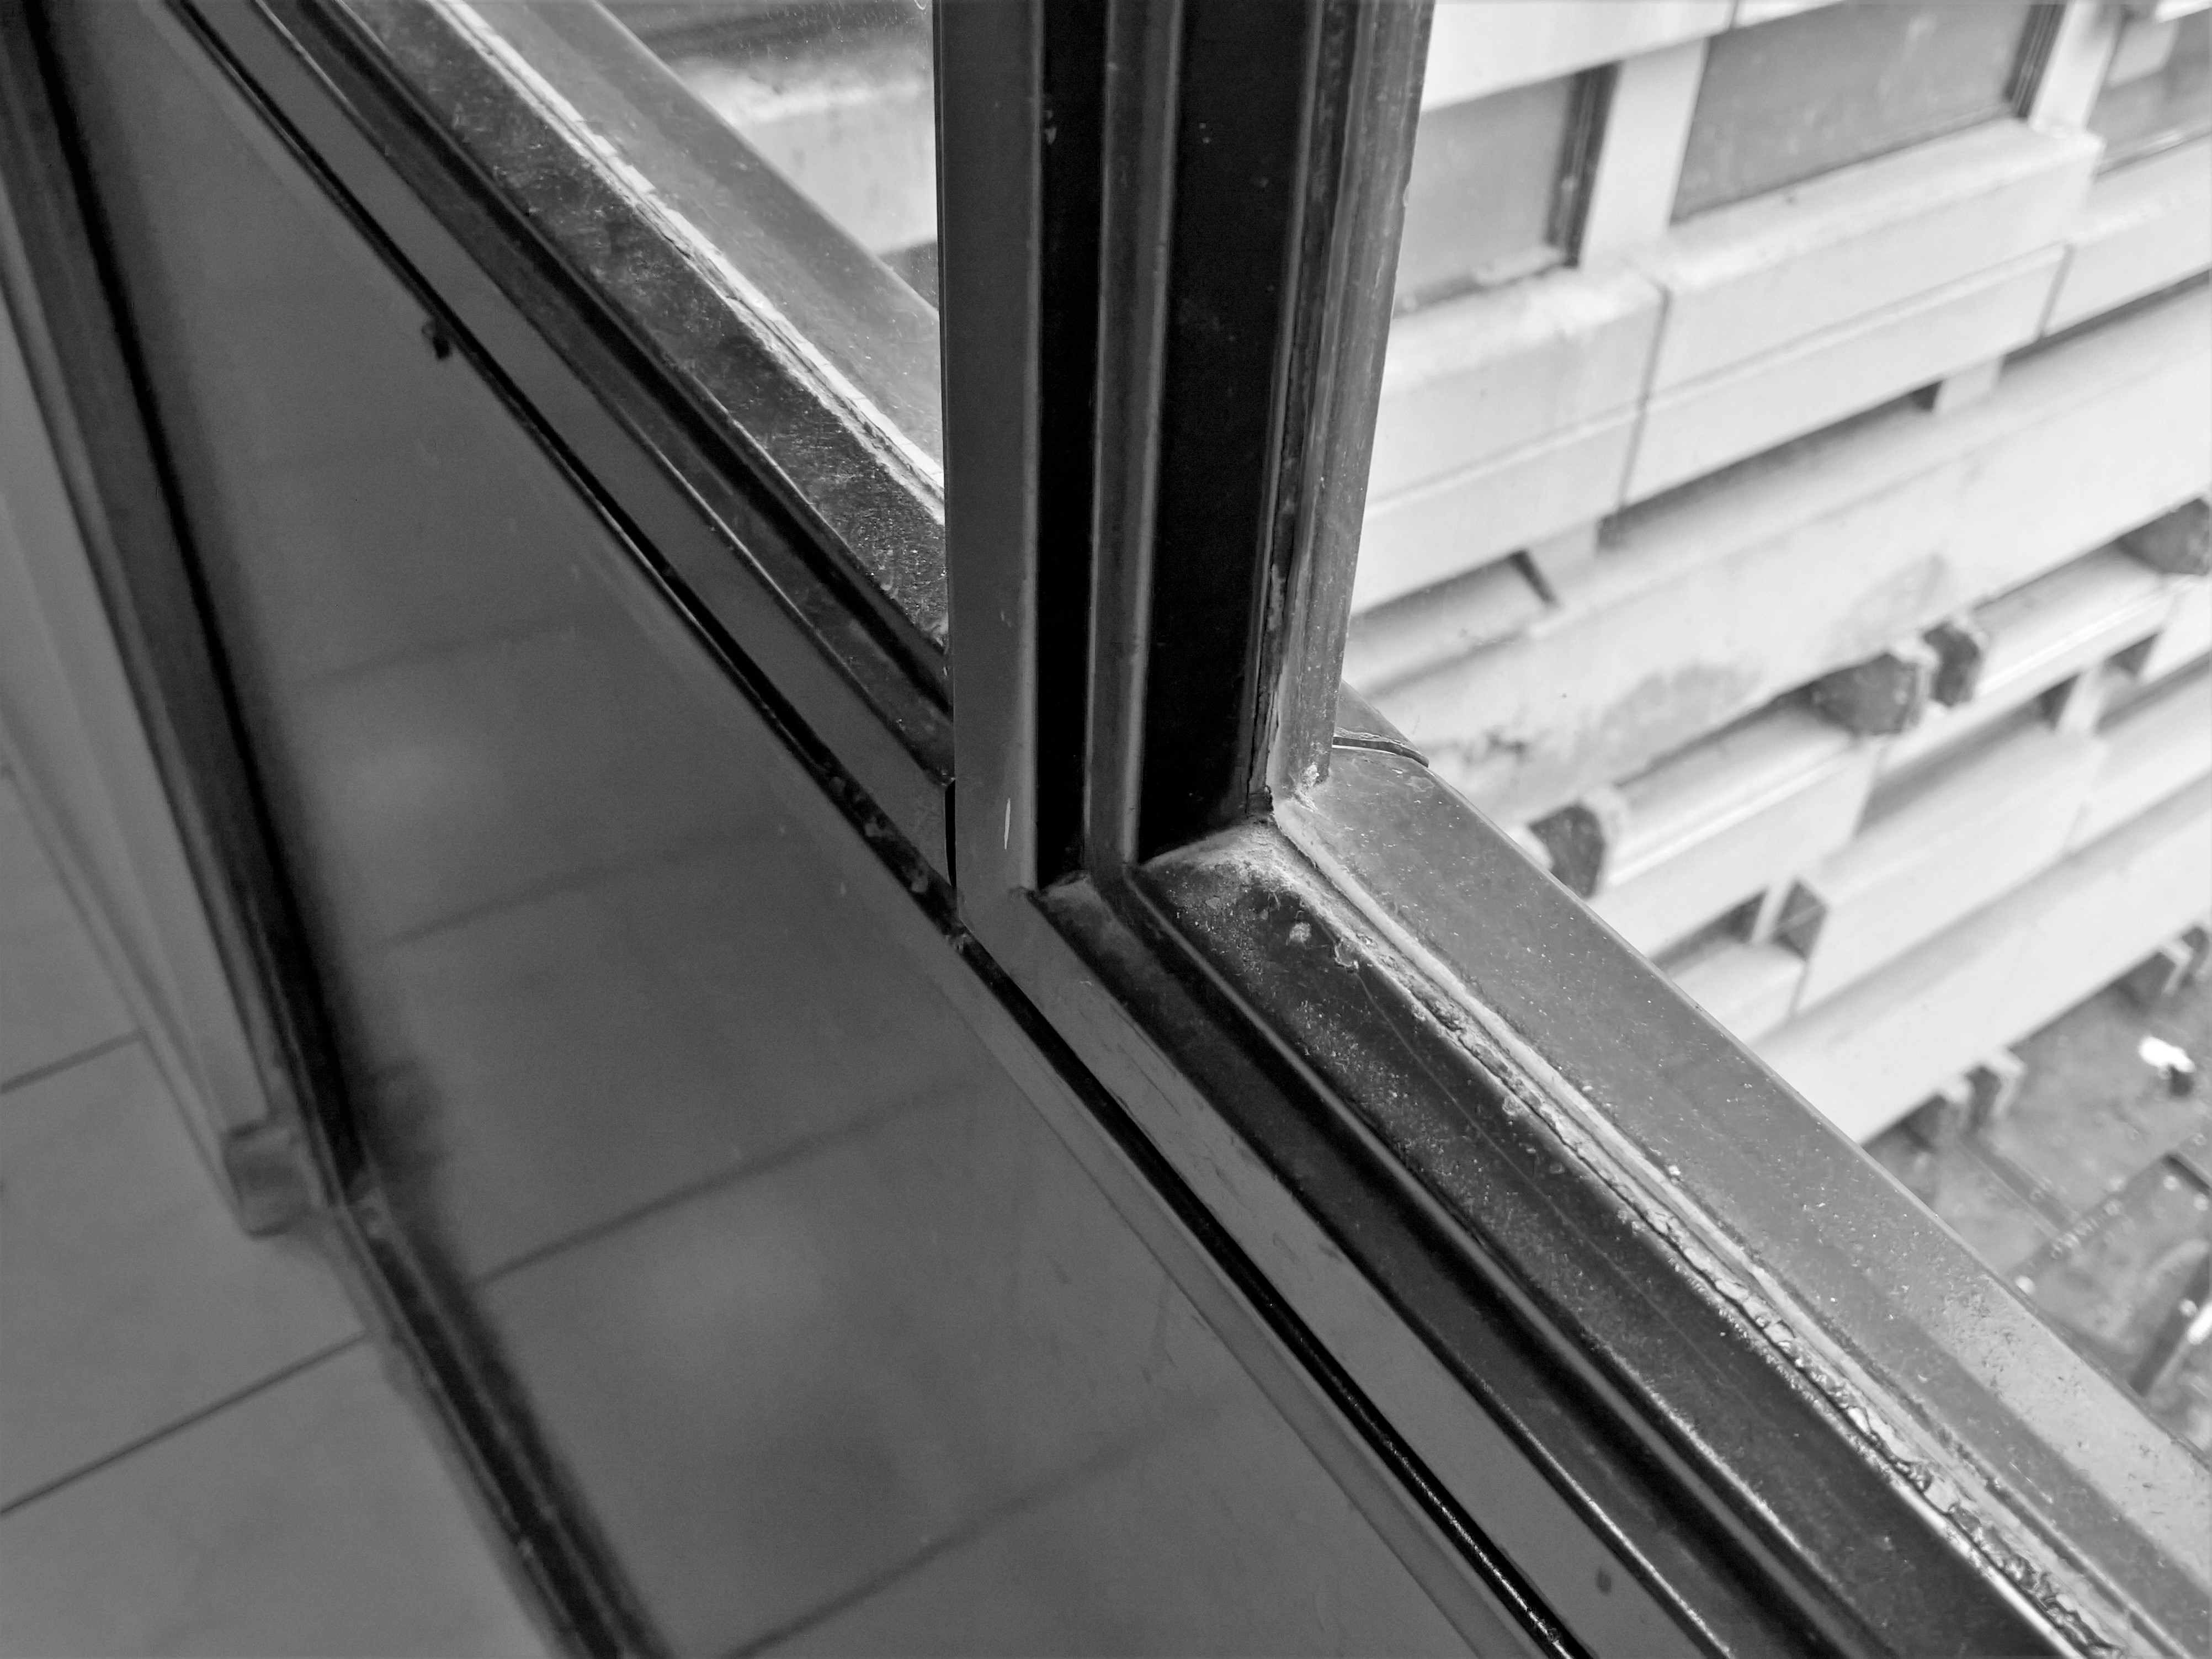
\includegraphics[width=\textwidth]{6_2_cap/img/fin1}
	\caption[Particolare del componente FIN-160]{Particolare del componente \textbf{FIN-160}: notare lo spessore di \n{4}{mm} della lastra di vetro.}\label{fin1}
\end{figure}

\begin{figure}[t]
	\centering
	\subfloat[][\emph{Una delle \textbf{PT-160} del corpo C. Sotto l'elemento di cemento armato ad U capovolto è presente \textbf{PT-Alta Corpo Basso}.}]{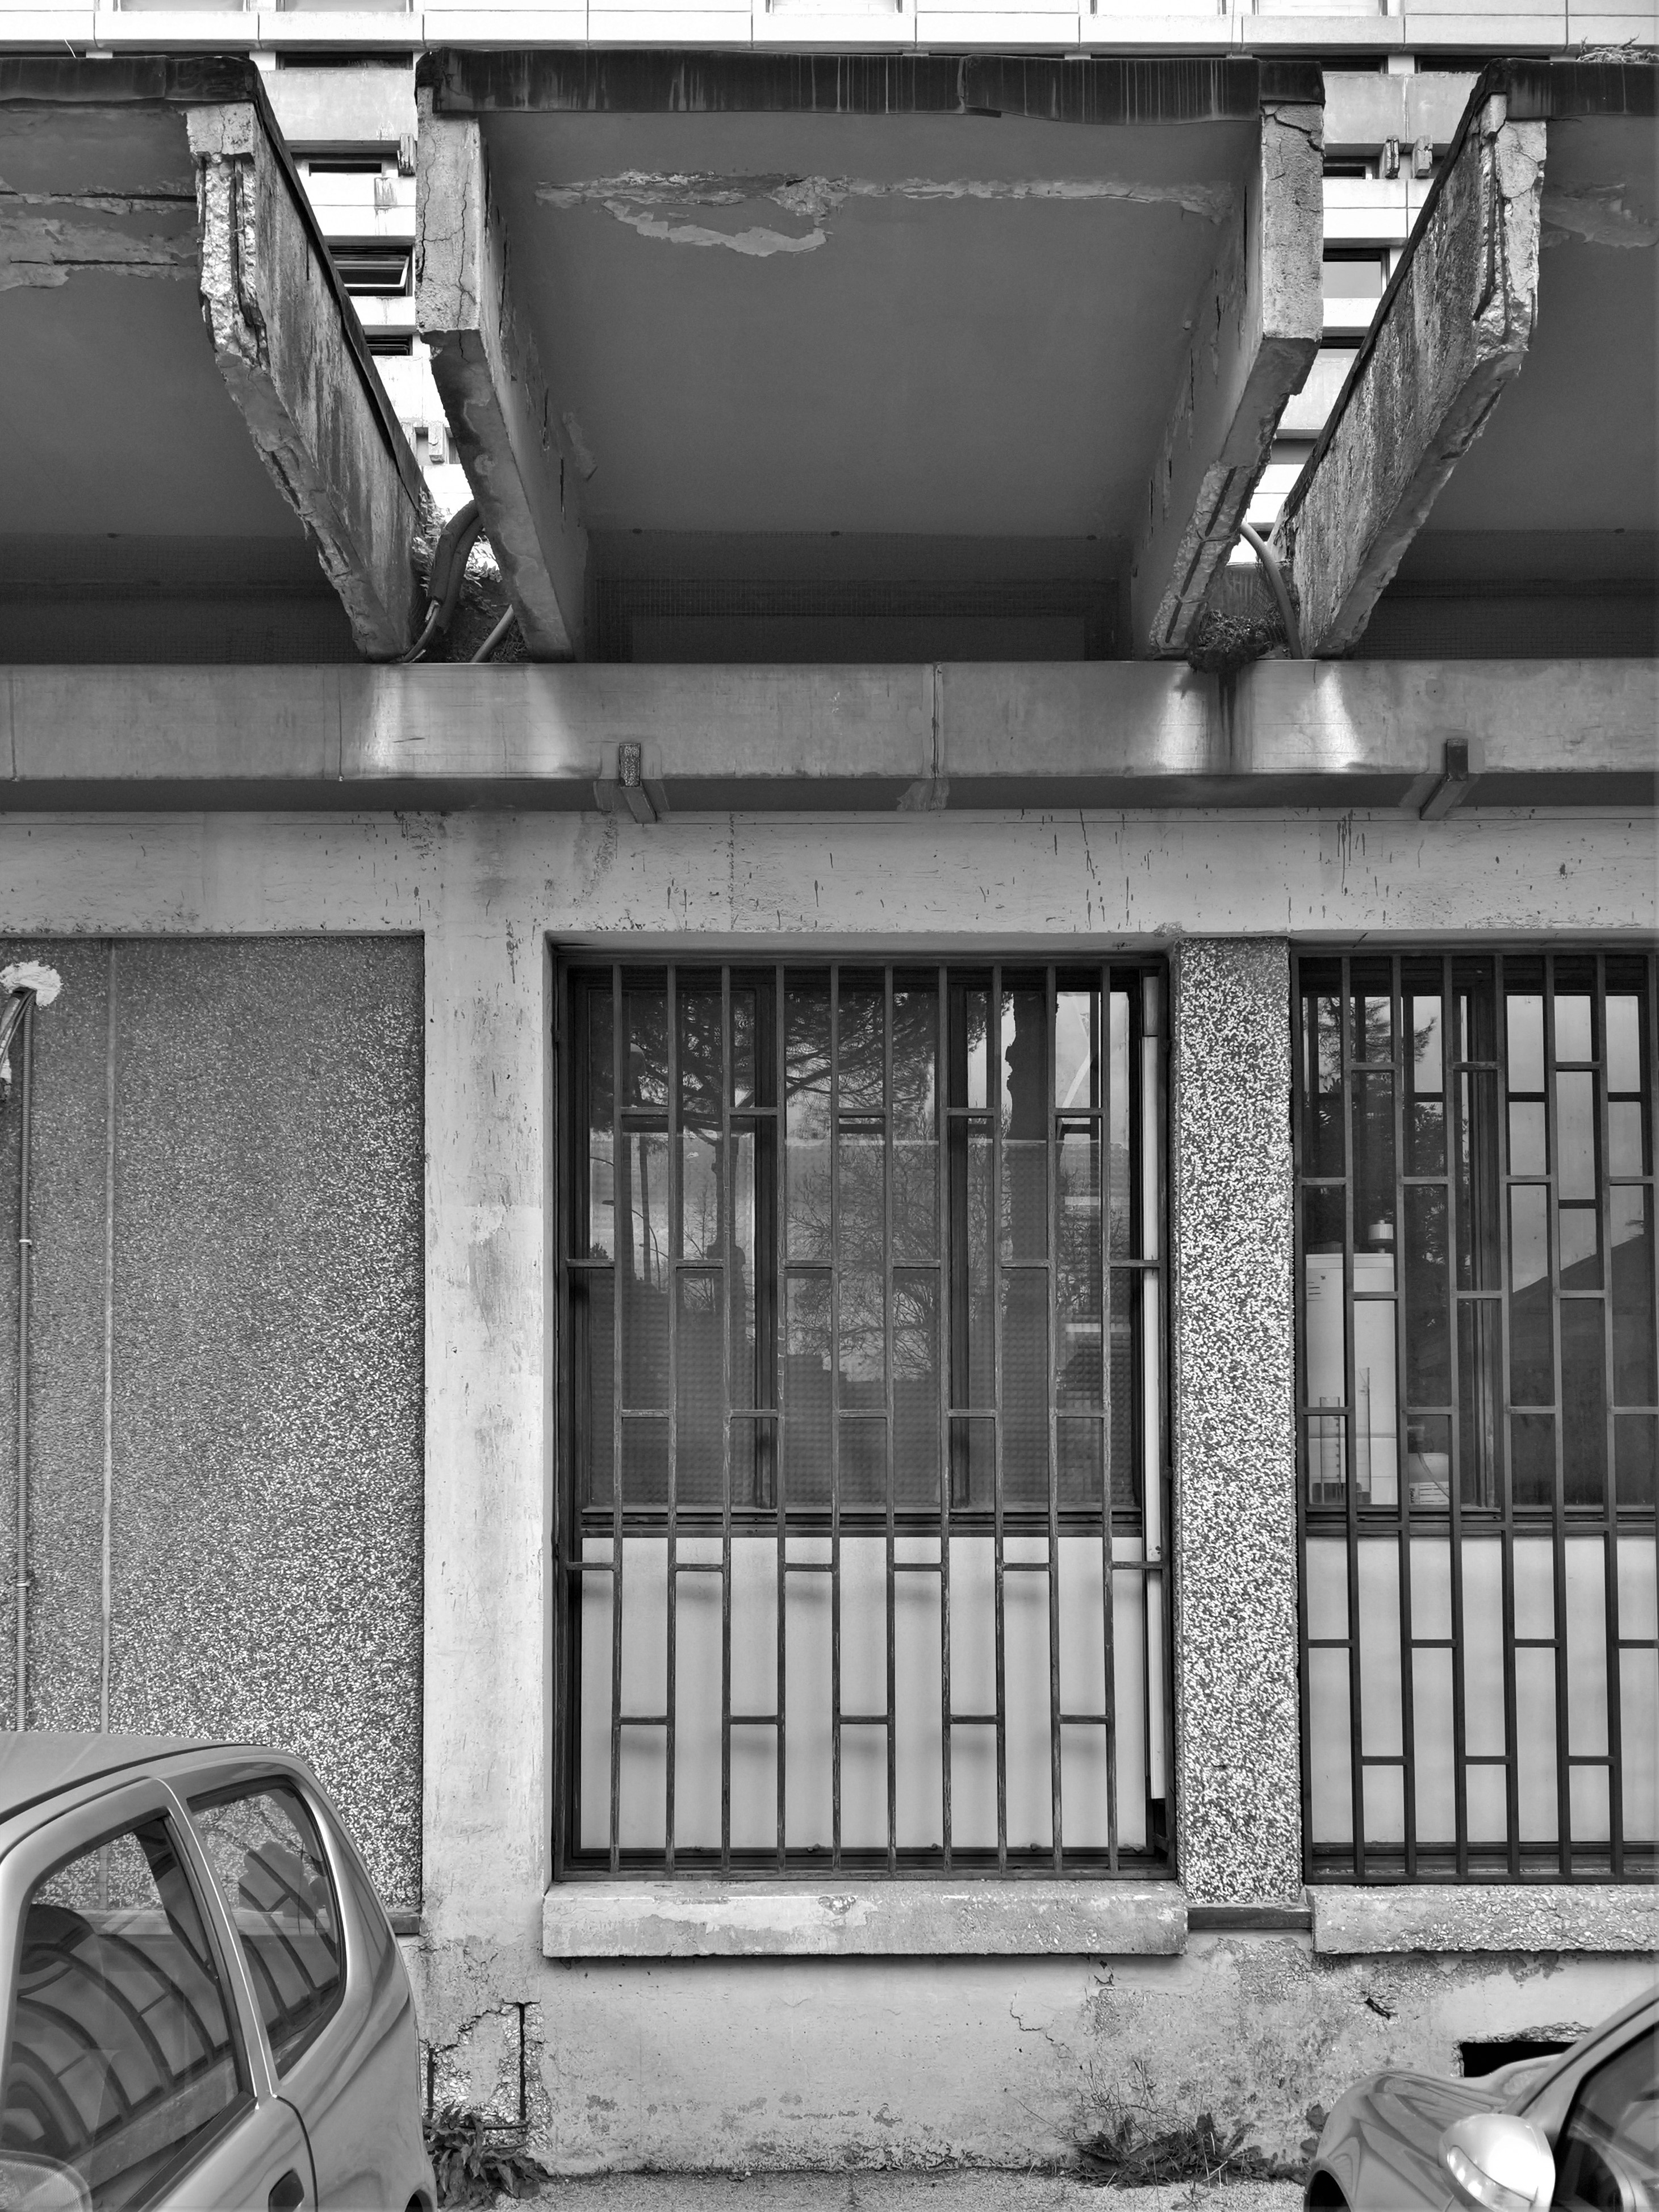
\includegraphics[width=0.35\textwidth]{6_2_cap/img/fincb}\label{fincb}} \quad
	\subfloat[][\emph{Due finestre \textbf{QUADRA}.}]{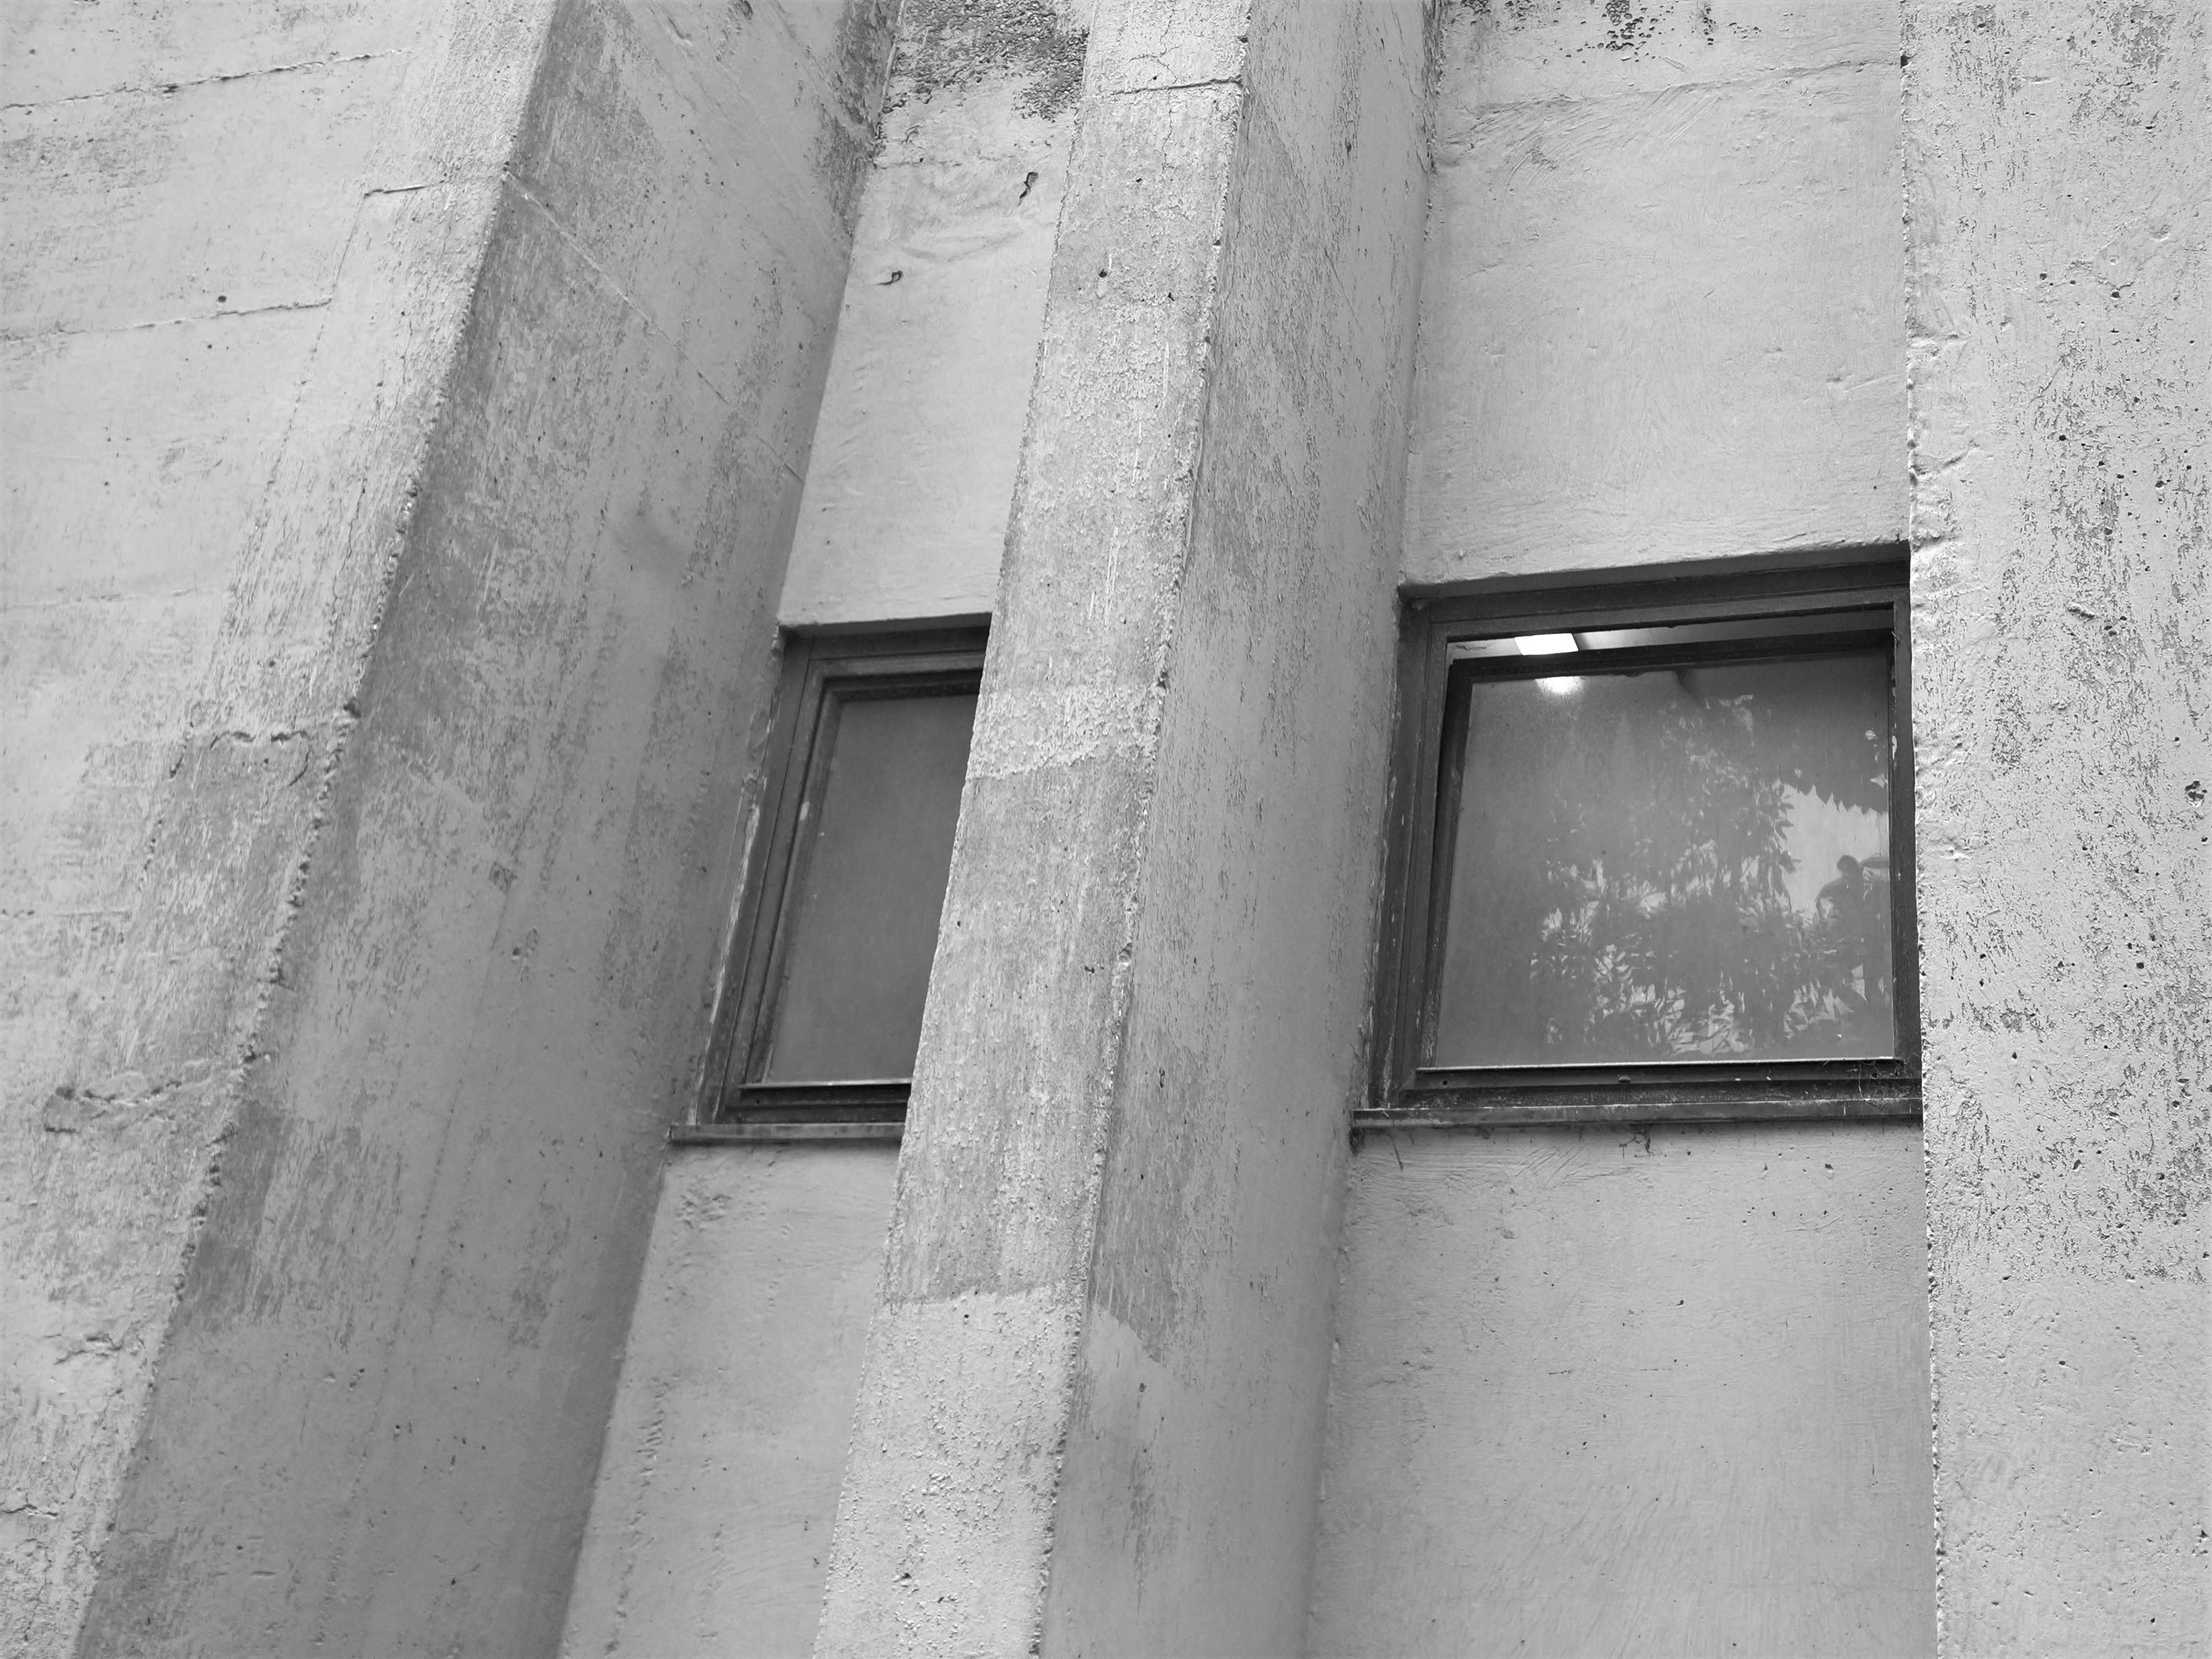
\includegraphics[width=0.35\textwidth]{6_2_cap/img/finq}\label{finq}} 
	\caption{Alcuni componenti trasparenti dell'edificio 2.}
\end{figure}

A conclusione dell'analisi si evidenzia come tutti i valori di trasmittanza calcolati sia per le strutture opache verticali che quelle orizzontali come anche i componenti trasparenti risultano sensibilmente superiori ai valori limite contenuti nel DM 26/6/2015.

\subsection{Definizione locali}
Il carico termico di un edificio (come anche il suo fabbisogno energetico) non tiene conto solamente dell'ambiente esterno (temperatura e umidità tutto l'anno mentre la radiazione solare solo in estate). È molto importante considerare la destinazione d'uso del locale che si intende climatizzare. Pertanto sono stati individuati le tipologie di locali e per ognuno di essi si sono definiti i seguenti parametri:
\begin{itemize}
	\item \emph{Temperatura} e \emph{umidità relativa} di progetto nella stagione estiva e invernale. Una loro adeguata scelta in fase progettuale e poi un loro mantenimento ad impianto ultimato e perfettamente funzionante sono alla base del benessere di una persona che vive in un locale;
	\item La \emph{portata di rinnovo} dalla norma \norvent. Rappresenta la quantità di aria esterna che si suppone essere priva di agenti nocivi per l'uomo e che è necessario introdurre all'interno dell'ambiente da climatizzare per mantenere entro certi limiti la qualità, appunto, dell'aria;
	\item Gli \emph{apporti interni di calore}:
	\begin{itemize}
		\item \emph{L'occupazione}, ovvero il numero di persone che affollano il locale con i conseguenti apporti di calore sensibile e latente. In assenza di dati certi (ovvero nell'impossibilità di conoscere le persone che effettivamente affollano un locale - contando il numero di posti a sedere in una sala di un cinema, per esempio) si procede utilizzando i valori di occupazione fissati dalla \norvent;
		\item \emph{Apparati interni}, ovvero i carichi dovuti a macchinari/fonti di calore sensibile e latente presenti all'interno del locale;
		\item \emph{L'illuminazione}, ovvero la quantità di calore sensibile (trasmesso per convezione e irraggiamento) dovuto all'illuminazione;
	\end{itemize}
\end{itemize}
È molto importante notare che per alcuni di questi apporti interni di calore sono stati definiti dei profili d'uso temporali su base oraria. \emph{L'occupazione} dello Studio Medico, per esempio, ha un profilo d'uso del tipo:
\begin{center}
	\begin{tabular}{lr}
		\toprule
		Dalle 00:00 alle 08:00 & 0\% \\
		Dalle 08:00 alle 17:00 & 100\% \\
		Dalle 17:00 alle 00:00 & 0\% \\
		\bottomrule
	\end{tabular}
\end{center}
Ovvero all'interno degli studi medici vi sarà il massimo dell'occupazione (calcolata considerando l'indice di affollamento $n_S$ che in questo caso è pari a \n{0.05}{pers/m^2} tratto sempre dalla \norvent) dalle 8:00 alle 17:00 ogni giorno dell'anno.

Un ulteriore aspetto da considerare è l'illuminazione dei locali a destinazione d'uso sanitaria. La maggior parte dei corpi illuminanti consiste in \emph{lampade a fluorescenza} avente efficienza luminosa di circa \n{80}{lm/W}. Dopo aver verificato la potenza effettivamente installata e note le superfici è stato possibile ricavare un indicatore in \si{W/m^2} per ogni locale. Qui di seguito i risultati utilizzati come dati di input:
\begin{itemize}
	\item \n{10}{W/m^2} negli uffici, studi medici, segreteria;
	\item \n{19}{W/m^2} negli ambulatori, laboratori, sale operatorie e degenza;
	\item \n{10}{W/m^2} nei corridoi, atri e sale d'attesa;
	\item \n{9}{W/m^2} nei depositi e magazzini;
	\item \n{8}{W/m^2} nei bagni, spogliatoi e lavatoi.
\end{itemize}

Si vogliono descrivere in maniera dettagliata alcune tipologie di locali che sono stati maggiormente utilizzati per la modellazione dell'edificio.

\newpage
\subsubsection{Degenza}
\begin{figure}[h]
	\centering
	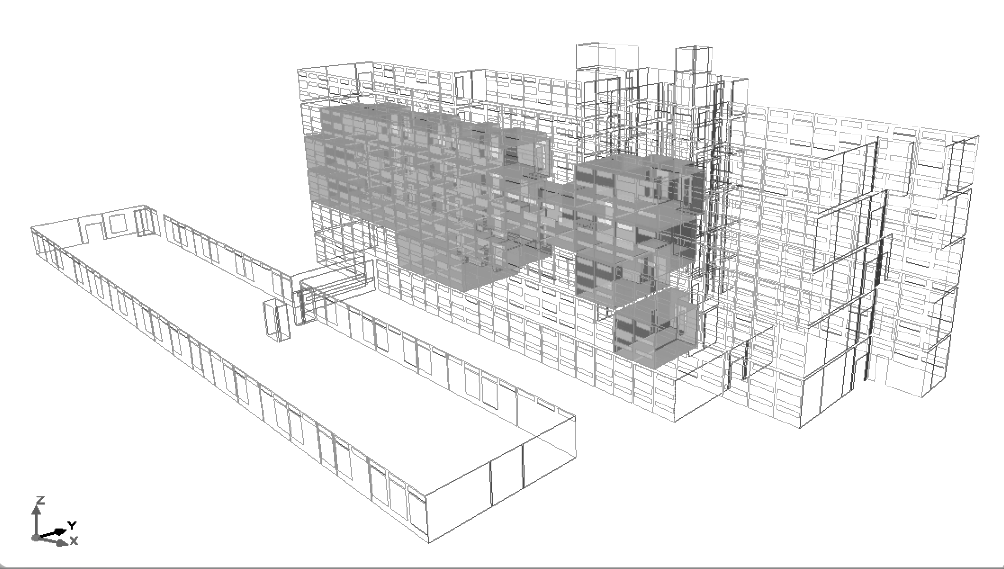
\includegraphics[height=0.5\textwidth]{6_2_cap/img/deg}
	\caption{Posizione delle degenze all'interno del corpo A.}\label{deg}
\end{figure}
\begin{center}
	\begin{tabular}{lcc}
										& Raffrescamento 			& Riscaldamento \\
		Temperatura interna di progetto & \n{24.0}{\degreeCelsius} 	& \n{21.0}{\degreeCelsius}\\
		Umidità interna di progetto 	& \n{50.0}{\%}				& \n{30.0}{\%}\\
		\midrule
		Ventilazione					& \multicolumn{2}{c}{\n{11}{l/s} per persona} 		\\
		\midrule
		\multirow{3}*{Occupazione}		& \multicolumn{2}{c}{\n{5}{m^2/pers}}  		\\
									 	& \n{75}{W/pers} 		& sensibile	\\
										& \n{70}{W/pers}		& latente 	\\
		\midrule
		Apparati interni 				&\n{15}{W/m^2}			& sensibile\\
		\midrule
		Illuminazione					& \multicolumn{2}{c}{\n{19}{W/m^2}}\\
		\midrule
		Altri carichi					& \multicolumn{2}{c}{--}\\				
	\end{tabular}
\end{center}

\newpage
\subsubsection{Laboratorio}
\begin{figure}[h]
	\centering
	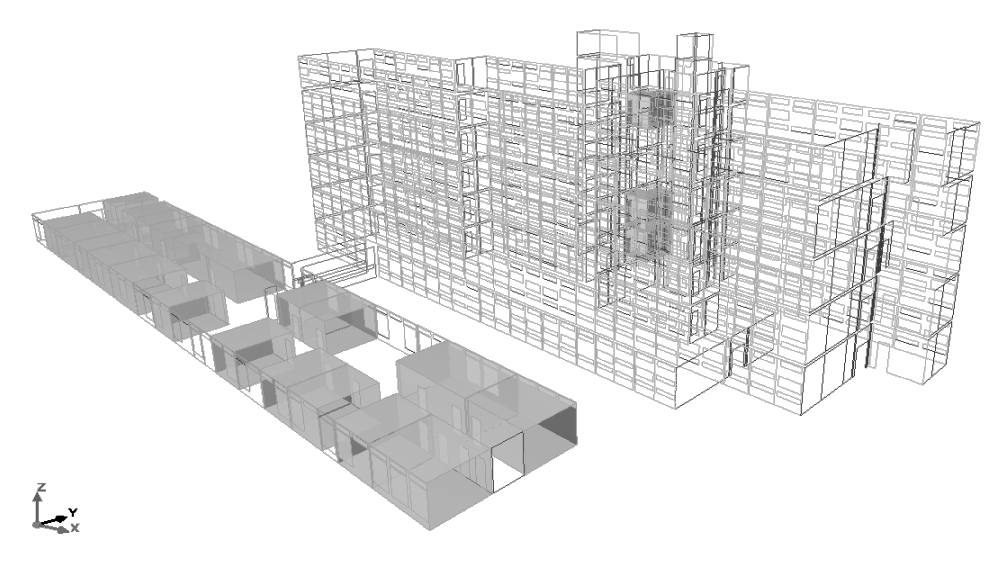
\includegraphics[height=0.5\textwidth]{6_2_cap/img/lab}
	\caption{Posizione dei laboratori nei corpi A e C.}\label{lab}
\end{figure}
\begin{center}
	\begin{tabular}{lcc}
										& Raffrescamento 			& Riscaldamento \\
		Temperatura interna di progetto & \n{25.0}{\degreeCelsius} 	& \n{21.0}{\degreeCelsius}\\
		Umidità interna di progetto 	& \n{50.0}{\%}				& \n{50.0}{\%}\\
		\midrule
		Ventilazione					& \multicolumn{2}{c}{\n{6}{vol/h}} 		\\
		\midrule
		\multirow{3}*{Occupazione}		& \multicolumn{2}{c}{\n{20}{m^2/pers}}  		\\
										& \n{75}{W/pers} 		& sensibile	\\
										& \n{55}{W/pers}		& latente 	\\
		\midrule
		Apparati interni 				&\n{40}{W/m^2}			& sensibile\\
		\midrule
		Illuminazione					& \multicolumn{2}{c}{\n{19}{W/m^2}}\\
		\midrule
		Altri carichi					& \n{1000}{W}			& sensibile \\				
	\end{tabular}
\end{center}

\newpage
\subsubsection{Studio Medico}
\begin{figure}[h]
	\centering
	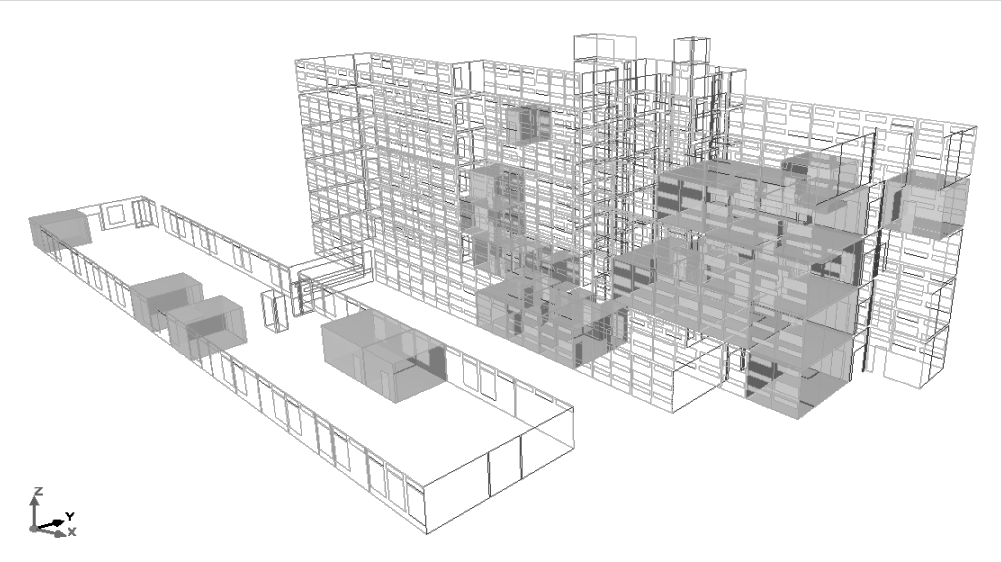
\includegraphics[height=0.5\textwidth]{6_2_cap/img/stm}
	\caption{Posizione degli studi medici nei corpi A e C.}\label{stm}
\end{figure}
\begin{center}
	\begin{tabular}{lcc}
										& Raffrescamento 			& Riscaldamento \\
		Temperatura interna di progetto & \n{25.0}{\degreeCelsius} 	& \n{22.0}{\degreeCelsius}\\
		Umidità interna di progetto 	& \n{50.0}{\%}				& \n{40.0}{\%}\\
		\midrule
		Ventilazione					& \multicolumn{2}{c}{\n{11}{l/s} per persona} 		\\
		\midrule
		\multirow{3}*{Occupazione}		& \multicolumn{2}{c}{\n{4}{pers}}  		\\
										& \n{75}{W/pers} 		& sensibile	\\
										& \n{55}{W/pers}		& latente 	\\
		\midrule
		Apparati interni 				&\multicolumn{2}{c}{--}\\
		\midrule
		Illuminazione					& \multicolumn{2}{c}{\n{10}{W/m^2}}\\
		\midrule
		Altri carichi					& \multicolumn{2}{c}{--}\\				
	\end{tabular}
\end{center}

\newpage
\subsubsection{Cucina}
\begin{figure}[h]
	\centering
	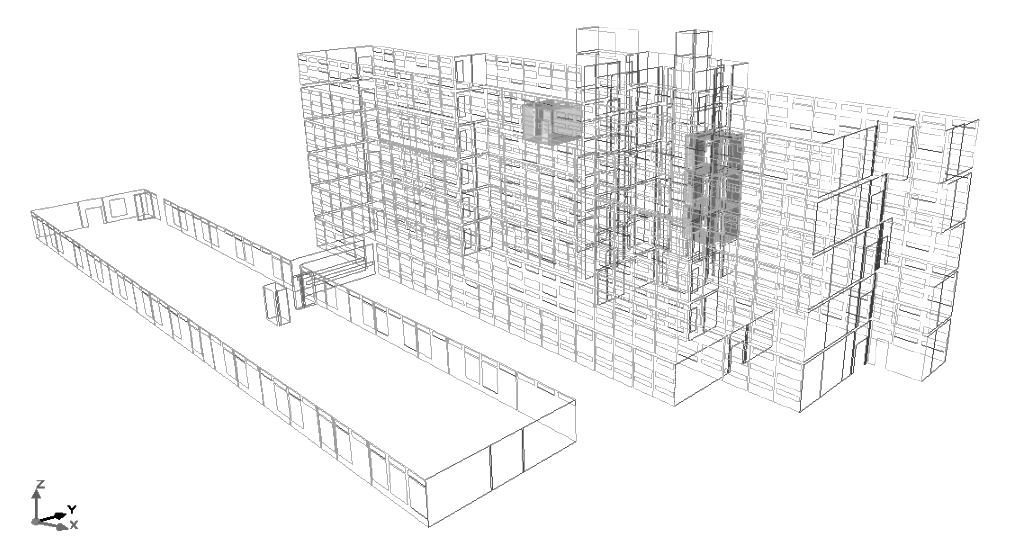
\includegraphics[height=0.5\textwidth]{6_2_cap/img/cuc}
	\caption{Posizione delle cucine nei corpi A e C.}\label{cuc}
\end{figure}
\begin{center}
	\begin{tabular}{lcc}
										& Raffrescamento 			& Riscaldamento \\
		Temperatura interna di progetto & \n{28.0}{\degreeCelsius} 	& \n{20.0}{\degreeCelsius}\\
		Umidità interna di progetto 	& \n{50.0}{\%}				& \n{30.0}{\%}\\
		\midrule
		Ventilazione					& \multicolumn{2}{c}{\n{16.5}{l/s} per \si{m^2}} 		\\
		\midrule
		\multirow{3}*{Occupazione}		& \multicolumn{2}{c}{\n{5}{m^2/pers}}  		\\
										& \n{75}{W/pers} 		& sensibile	\\
										& \n{70}{W/pers}		& latente 	\\
		\midrule
		Apparati interni 				& \n{5.40}{W/m^2} 		& sensibile \\
		\midrule
		Illuminazione					& \multicolumn{2}{c}{\n{10}{W/m^2}}\\
		\midrule
		\multirow{2}{*}{Altri carichi}	& \n{1500}{W} 		& sensibile \\
										& \n{500}{W} 		& latente   \\
	\end{tabular}
\end{center}

\newpage
\subsubsection{Ufficio}
\begin{figure}[h]
	\centering
	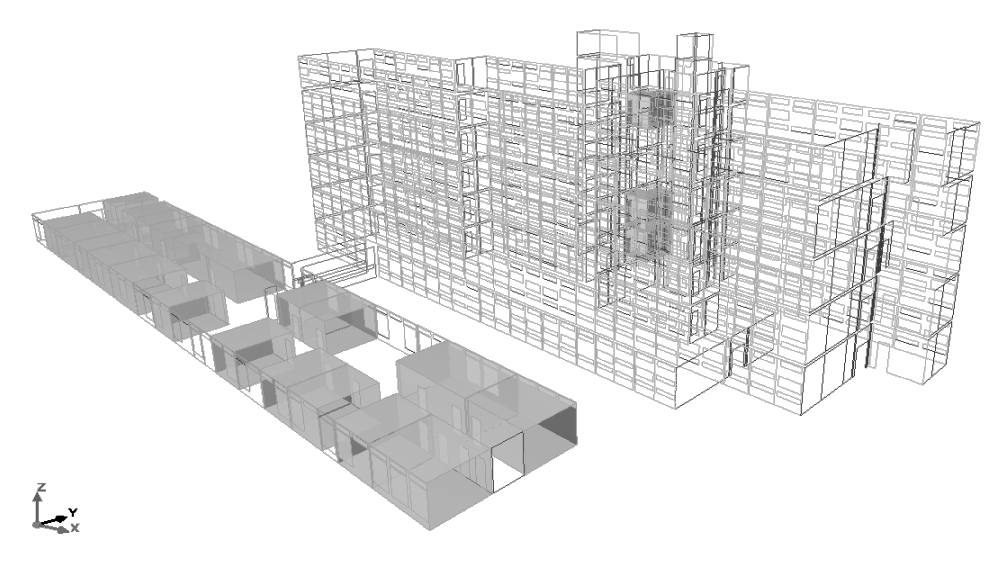
\includegraphics[height=0.5\textwidth]{6_2_cap/img/lab}
	\caption{Posizione degli uffici nei corpi A e C.}\label{uff}
\end{figure}
\begin{center}
	\begin{tabular}{lcc}
										& Raffrescamento 			& Riscaldamento \\
		Temperatura interna di progetto & \n{25.0}{\degreeCelsius} 	& \n{21.0}{\degreeCelsius}\\
		Umidità interna di progetto 	& \n{50.0}{\%}				& \n{40.0}{\%}\\
		\midrule
		Ventilazione					& \multicolumn{2}{c}{\n{11}{l/s} per persona} 		\\
		\midrule
		\multirow{3}*{Occupazione}		& \multicolumn{2}{c}{\n{10}{m^2/pers}}  		\\
										& \n{75}{W/pers} 		& sensibile	\\
										& \n{70}{W/pers}		& latente 	\\
		\midrule
		Apparati interni 				& \n{15}{W/m^2} 		& sensibile \\
		\midrule
		Illuminazione					& \multicolumn{2}{c}{\n{10}{W/m^2}}\\
		\midrule
		Altri carichi					& \multicolumn{2}{c}{--}\\
	\end{tabular}
\end{center}

\newpage
\section{L'impianto}
L'impianto dell'Edificio 2 è attualmente caratterizzato da una sottocentrale, presente nel piano \num{-1}, la quale alimenta varie unità locali (radiatori e fancoil) e UTA oltre a produrre (tramite due bollitori da \n{5000}{l} ciascuno) acqua calda sanitaria.

Nel primo capitolo è già stato ampiamente detto che i vari edifici del Policlinico sfruttano la rete di presidio di acqua surriscaldata e refrigerata.

Partendo dal lato utenza, il carico sensibile invernale viene coperto da radiatori (si veda la \subref{radiatori} in \vref{unitloca}) presenti all'interno di ogni piano e fancoil solo nel III e IV piano. Il carico estivo (sia sensibile che latente) invece viene coperto da monosplit e fancoil ad acqua montati negli ultimi anni durante varie ristrutturazioni (come nel caso del terzo e quarto piano). In questi due piani vi è anche una rete aeraulica per il rinnovo dell'aria. Nonostante la presenza di questi impianti, non vengono garantiti l'adeguato recupero energetico dall'impianto di ventilazione e il controllo termo-igrometrico dai fancoil e radiatori. Queste carenze sono evidenti nell'eccessivo ricorso a split per il controllo della temperatura (e in modo indiretto dell'umidità) durante la stagione estiva. È evidente la necessità di una riqualificazione. Negli altri 3 piani la ventilazione è garantita tramite infiltrazione naturale (ovvero apertura delle finestre di piano) mentre è assente del tutto il controllo termo-igrometrico nella stagione estiva. Anche in questi piani si è fatto largo uso di monosplit a parete.

\begin{figure}[h!]
	\centering
	\subfloat[][\emph{Un tipico radiatore presente nel corridoio del Piano Terra -- Corpo A.}]{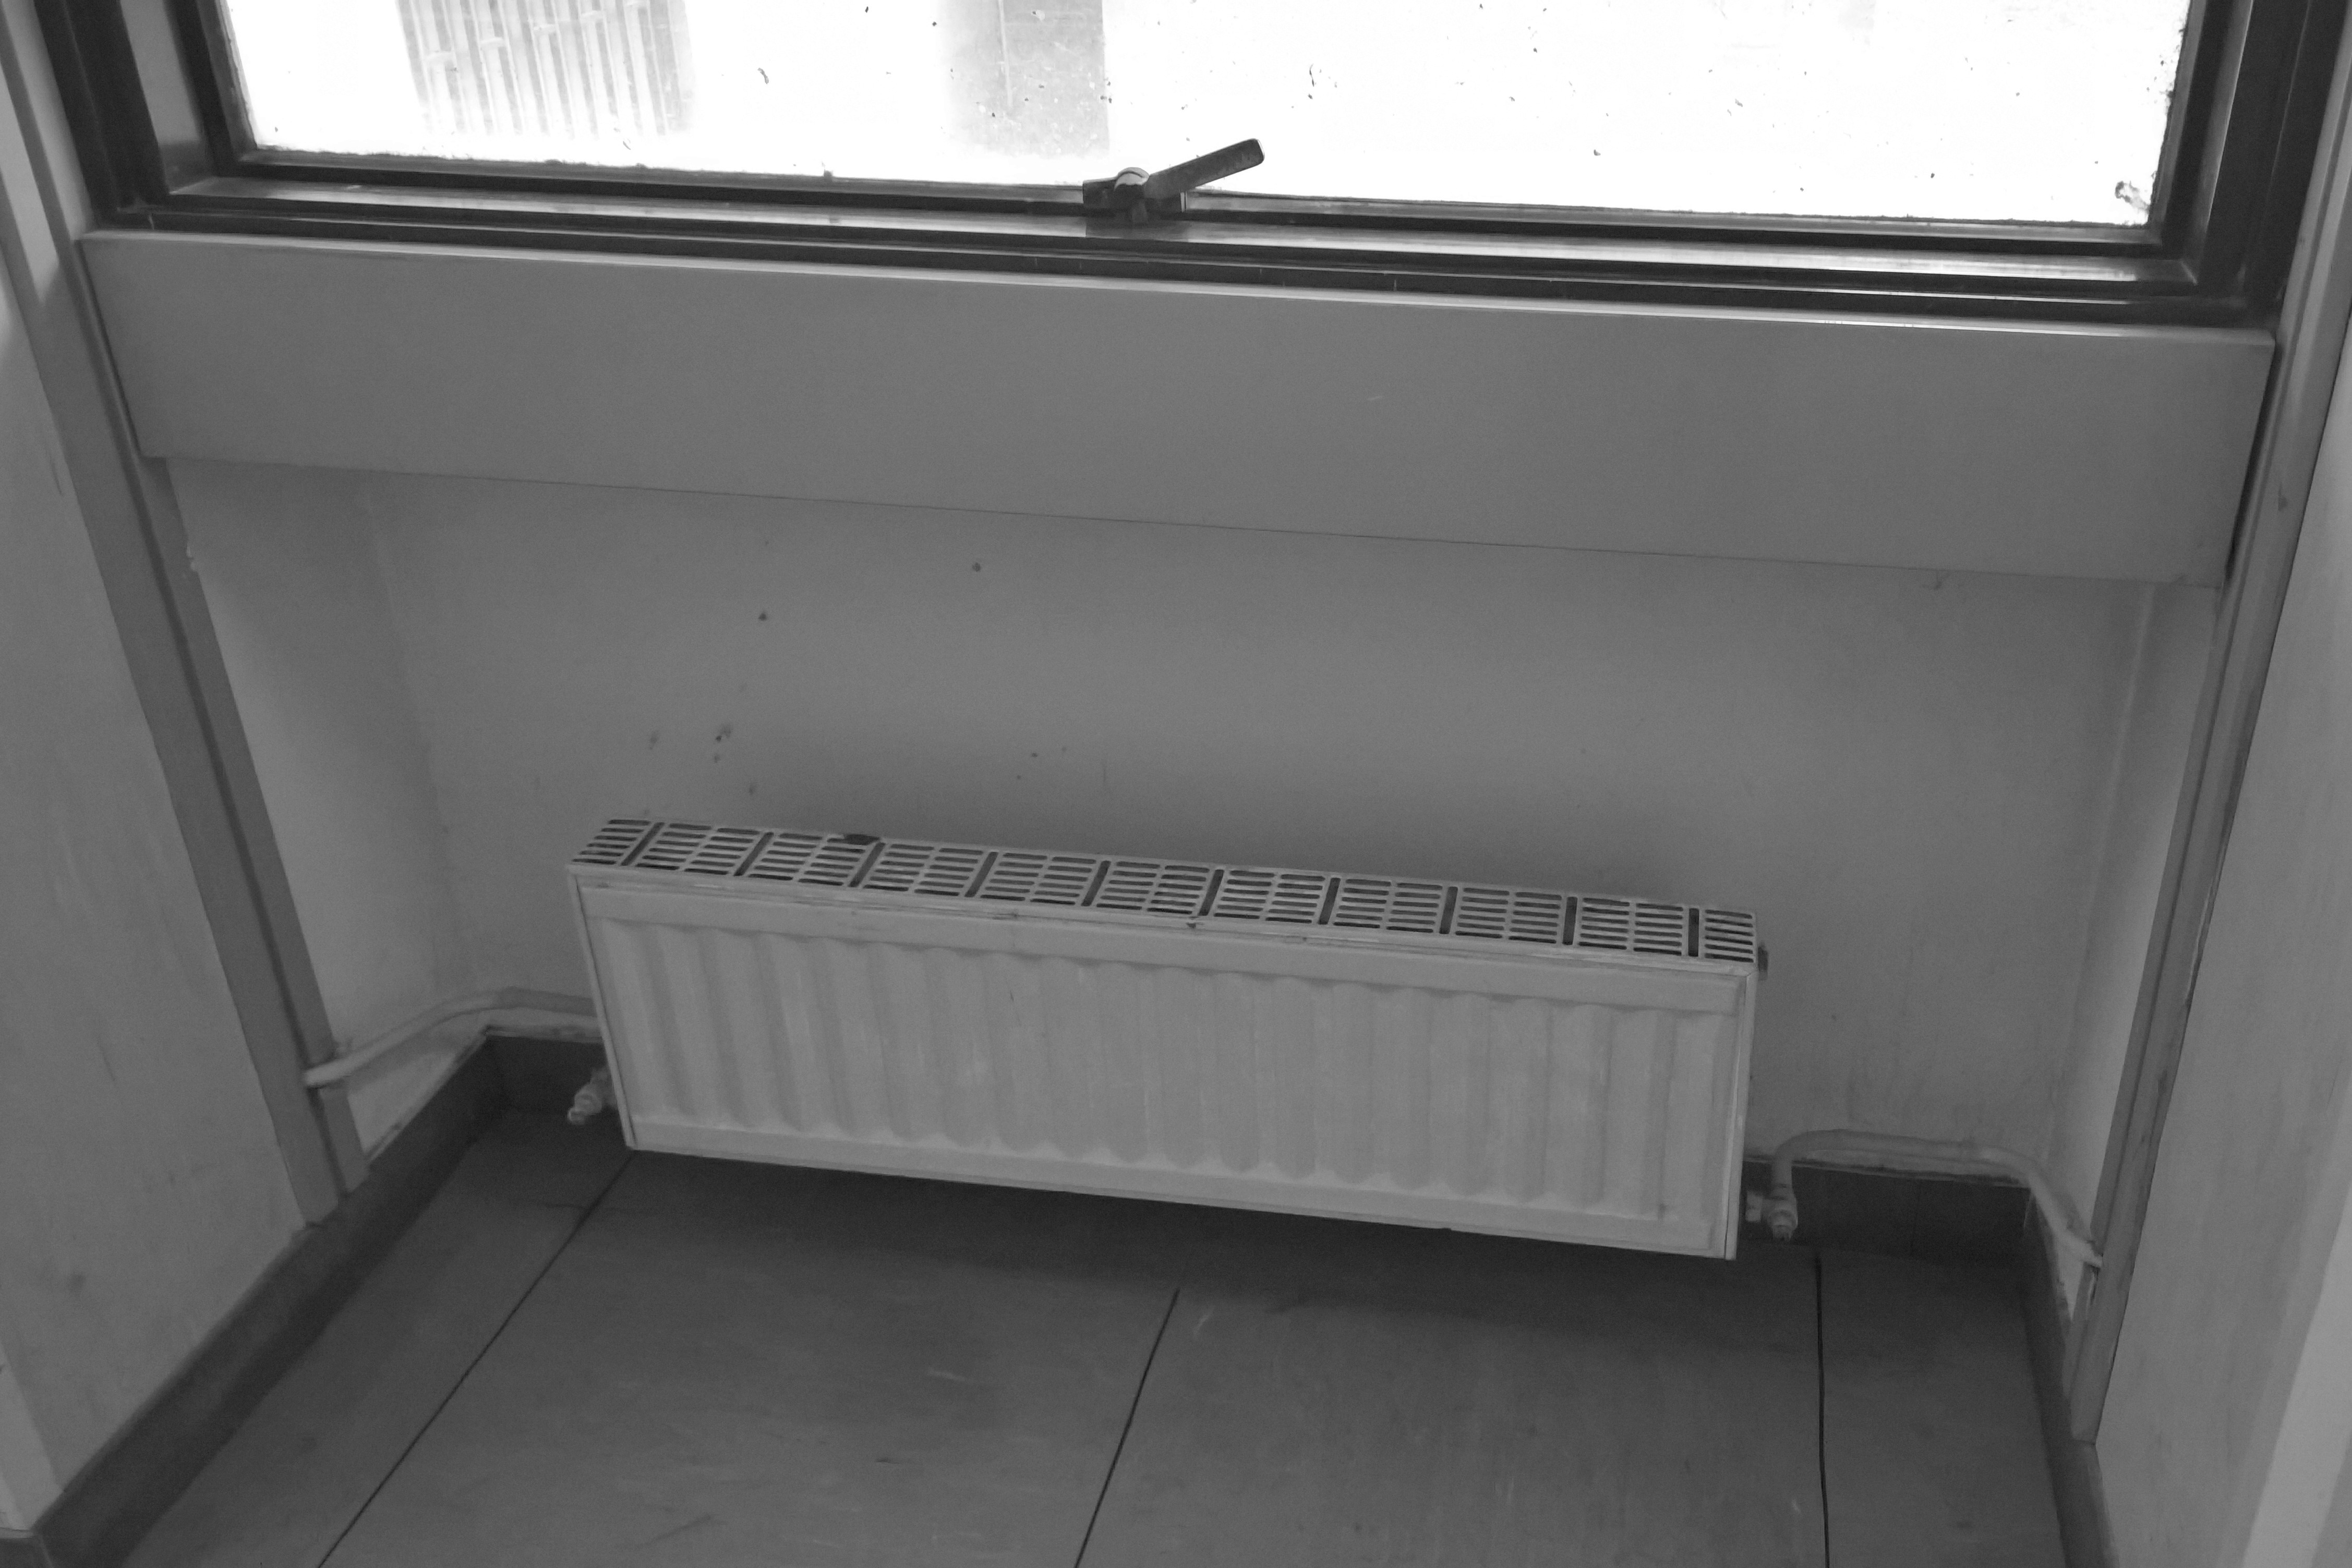
\includegraphics[width=0.45\textwidth]{6_2_cap/img/radiatore}\label{radiatori}}	\quad
	\subfloat[][\emph{Corridoio del IV Piano. Si noti il mix di unità locali.}]{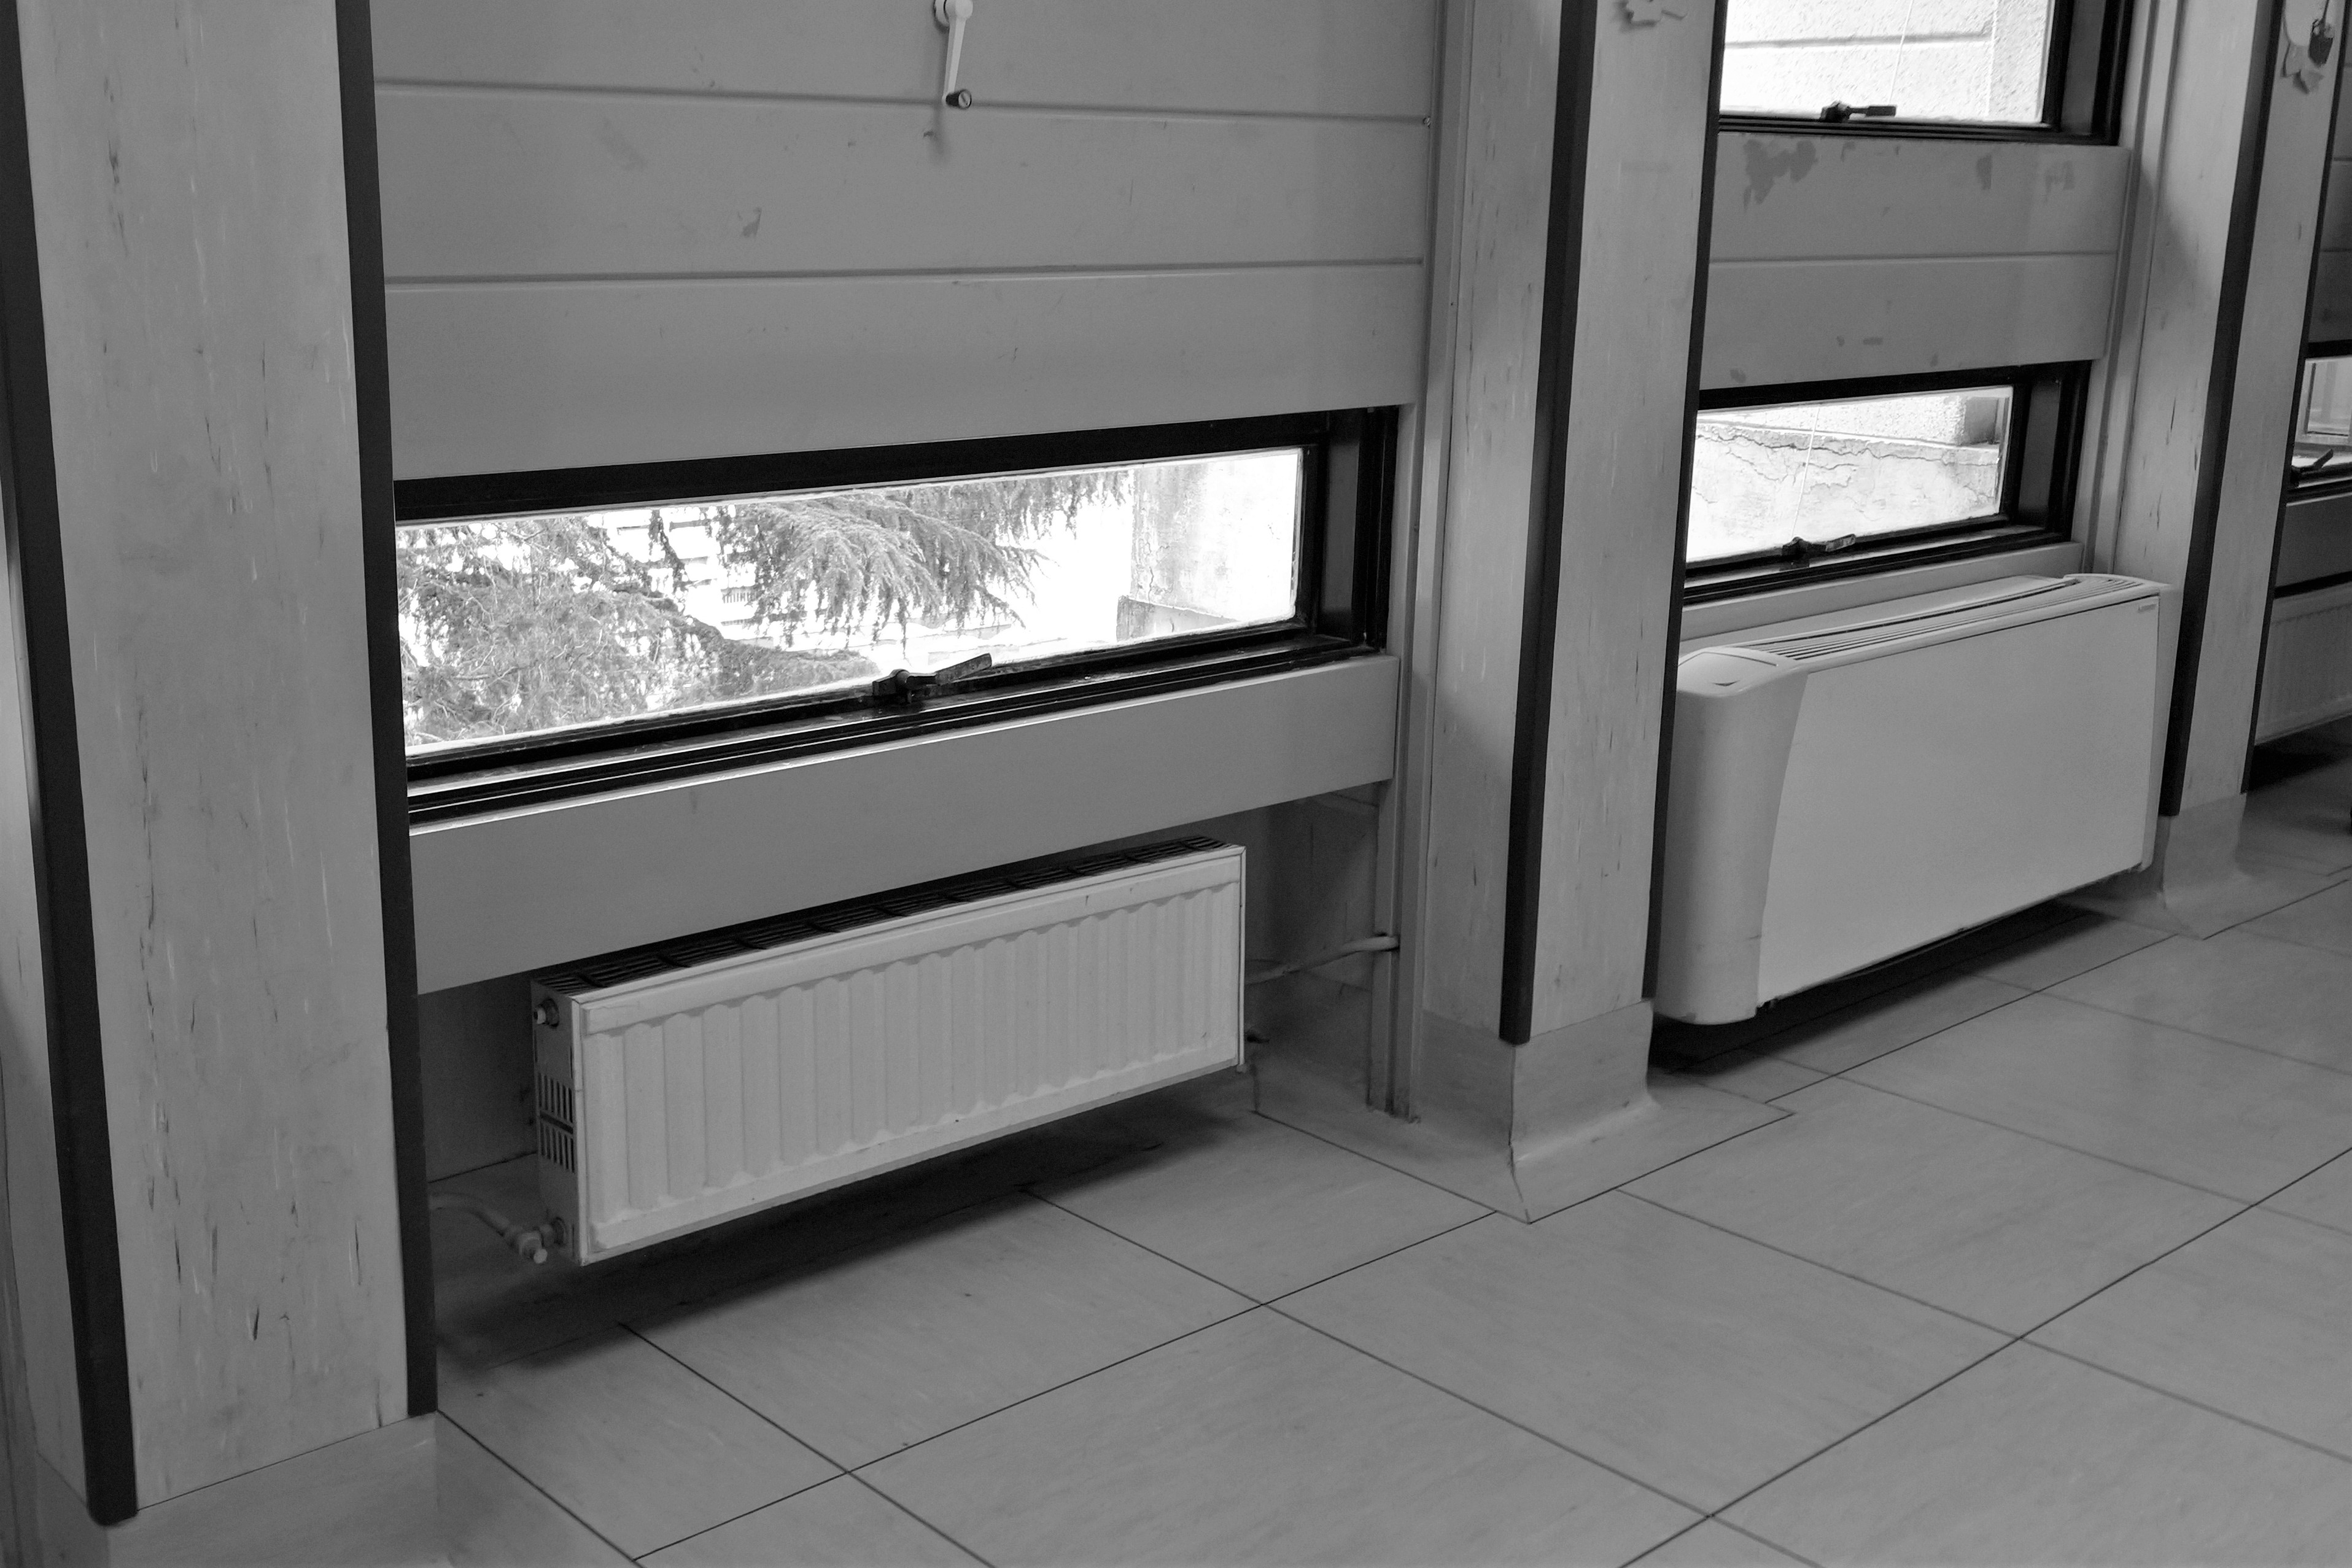
\includegraphics[width=0.45\textwidth]{6_2_cap/img/P4RadFan}}	\\
	\subfloat[][\emph{Area Relax del IV Piano. In alto la griglia di mandata del fancoil. Questi hanno anche una presa di aria di rinnovo esterna.}]{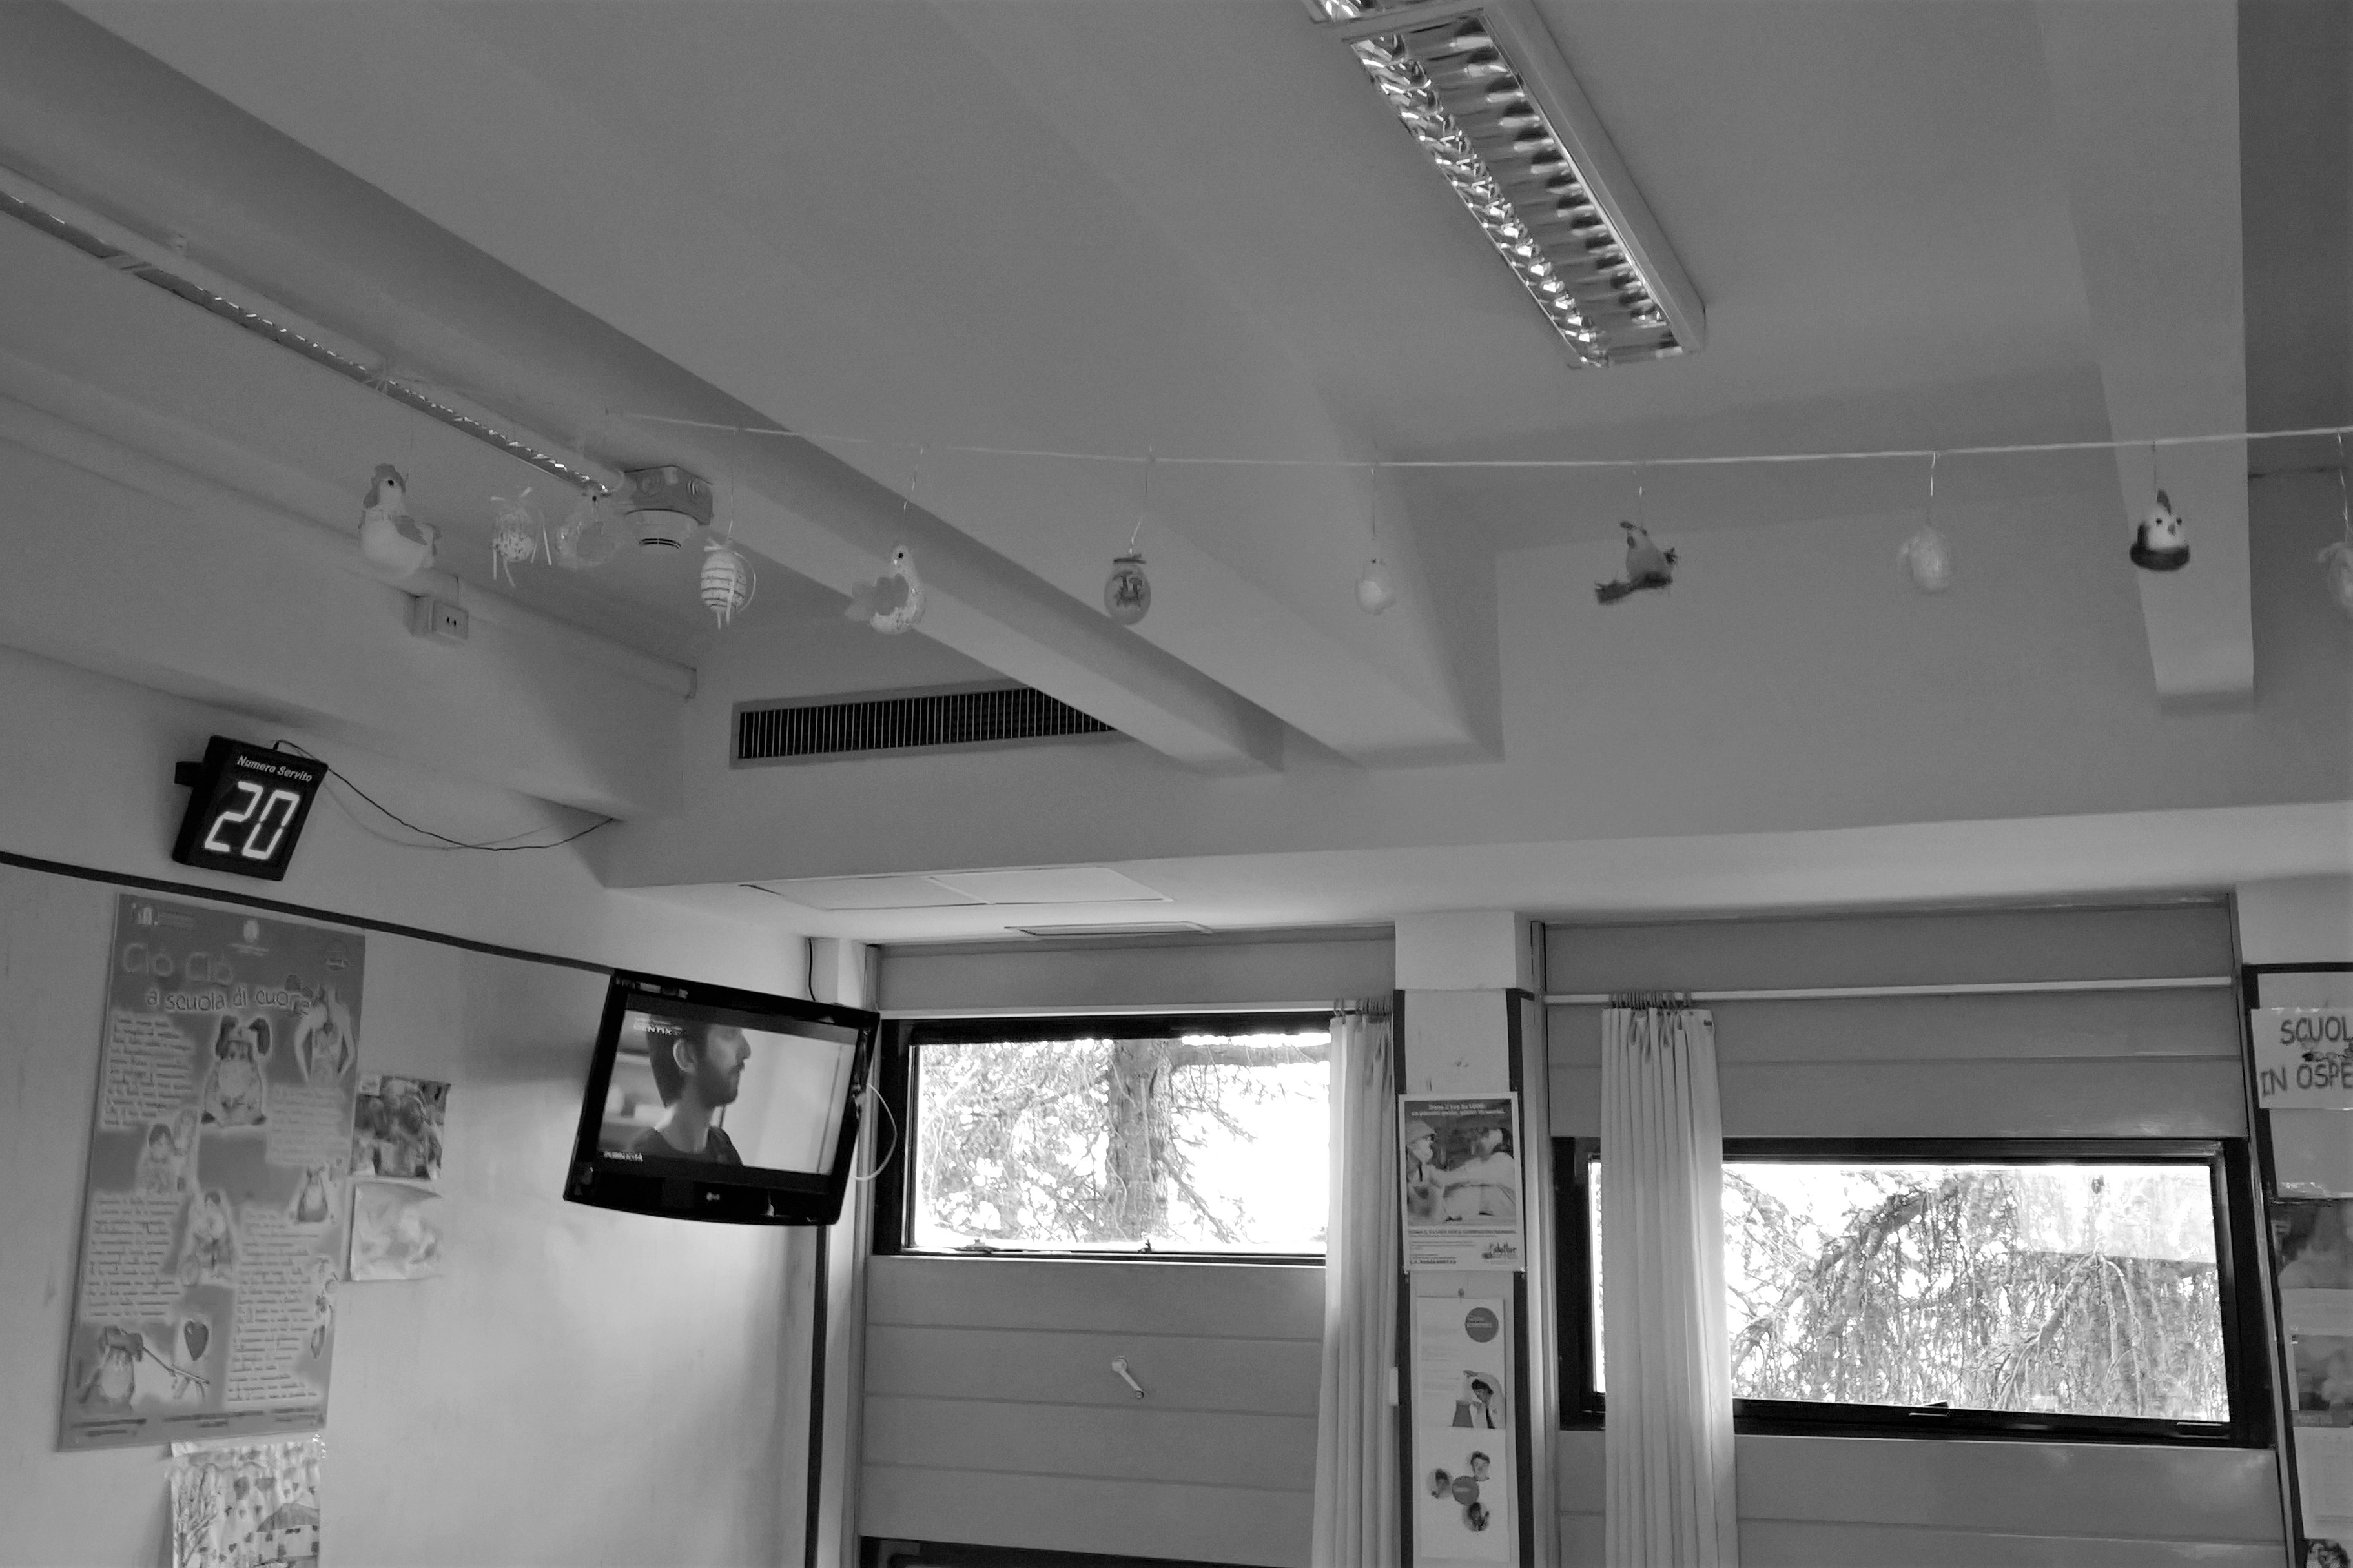
\includegraphics[width=0.45\textwidth]{6_2_cap/img/P4FanCoil}} \quad
	\subfloat[][\emph{Diffusore circolare in una degenza del III Piano per l'aria di rinnovo.}]{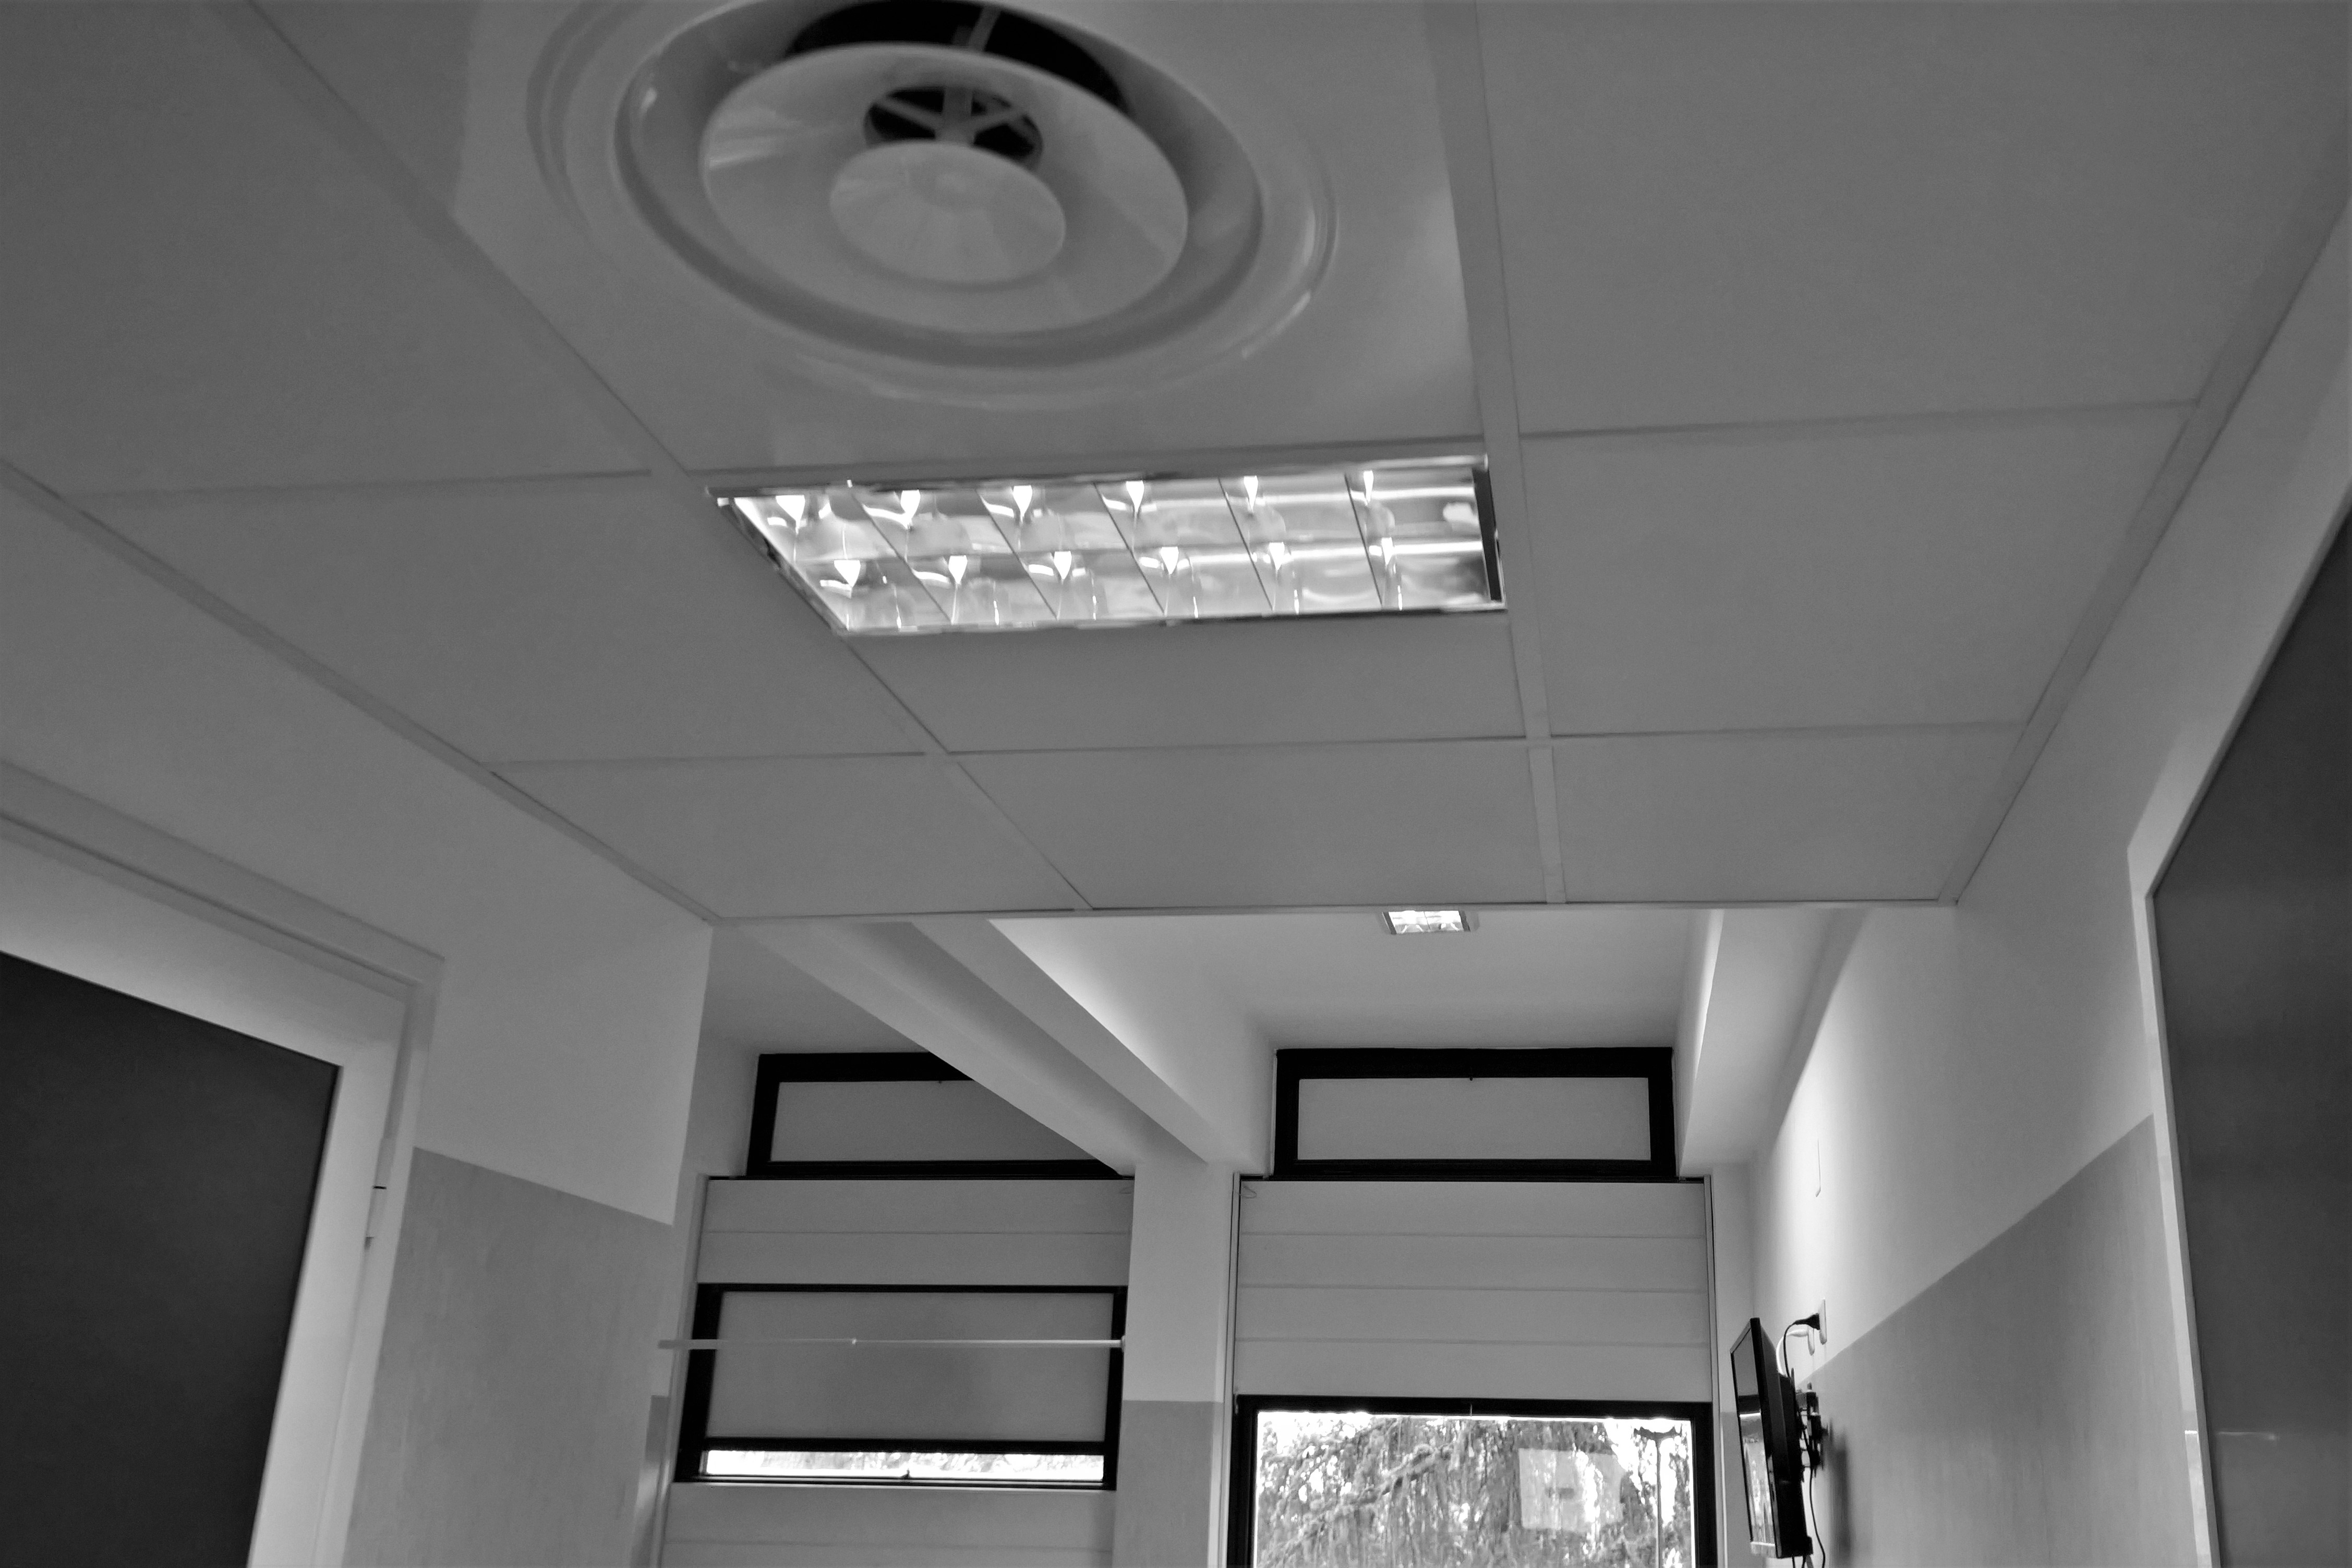
\includegraphics[width=0.45\textwidth]{6_2_cap/img/P3Aer}}
	\caption{Unità Locali nel Corpo A}\label{unitloca}
\end{figure}
	
Il quinto piano (in cui è presente il blocco operatorio di cardiochirurgia) è gestito da un adeguato impianto a tutt'aria presente in copertura.

In una porzione del primo piano vi è l'UTIC (\emph{Unità di Terapia Intensiva Coronarica}) che è trattata da un altro impianto a tutt'aria montato in un locale dello stesso piano. L'UTA dell'Emodinamica (al Piano Terra) con la relativa centrale termo-frigorifera è presente all'esterno.

Nonostante siano state elencati e descritti gli usi dei diversi edifici, l'intervento di riqualificazione energetica riguarda solo i corpi C e A. Di quest'ultimo edificio è escluso \emph{in toto} il blocco operatorio presente al quinto piano mentre dell'UTIC e dell'Emodinamica verrà effettuato solo un intervento civile (ovvero non verrà intaccato l'impianto aeraulico).

In \vref{img:PT}, \vref{img:P1}, \vref{img:P2}, \vref{img:P3} e \vref{img:P4} si riportano le planimetrie con le aree di intervento dei singoli piani.

%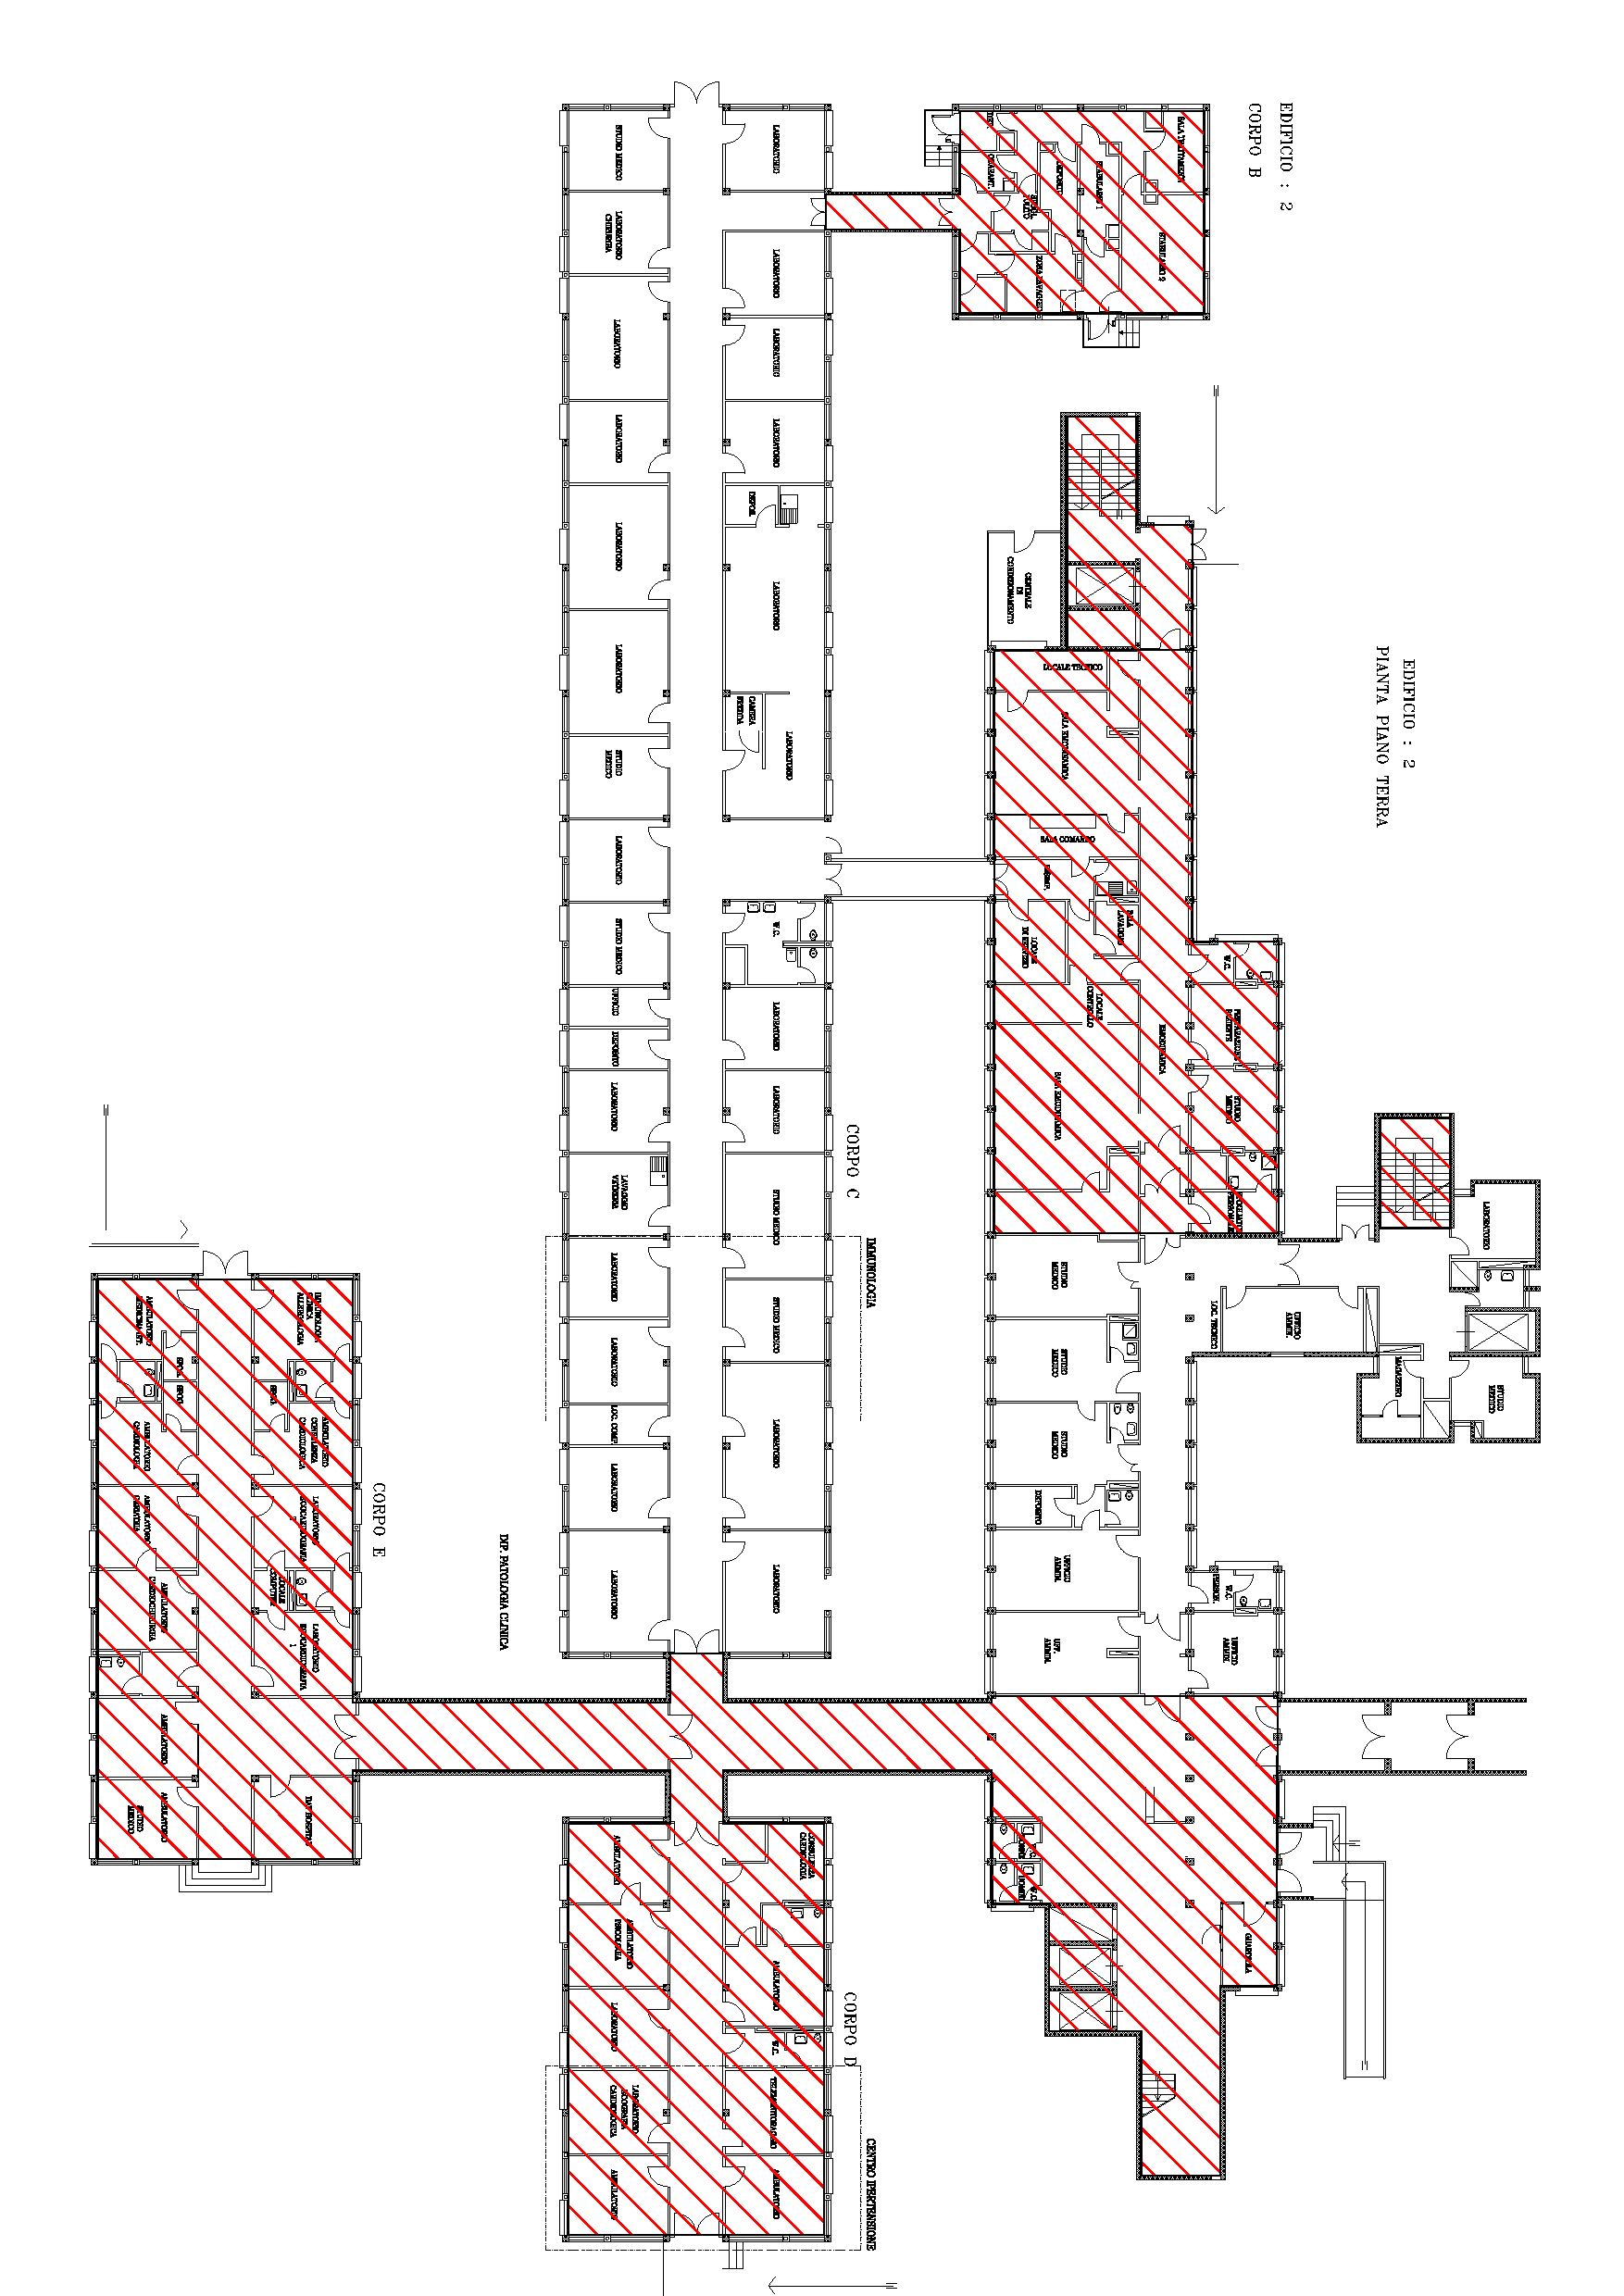
\includepdf[pagecommand={\null\vfill\captionof{table}{caioooo}}]{6_2_cap/img/PT.pdf}\label{PT}
\begin{sidewaysfigure}
	\centering
		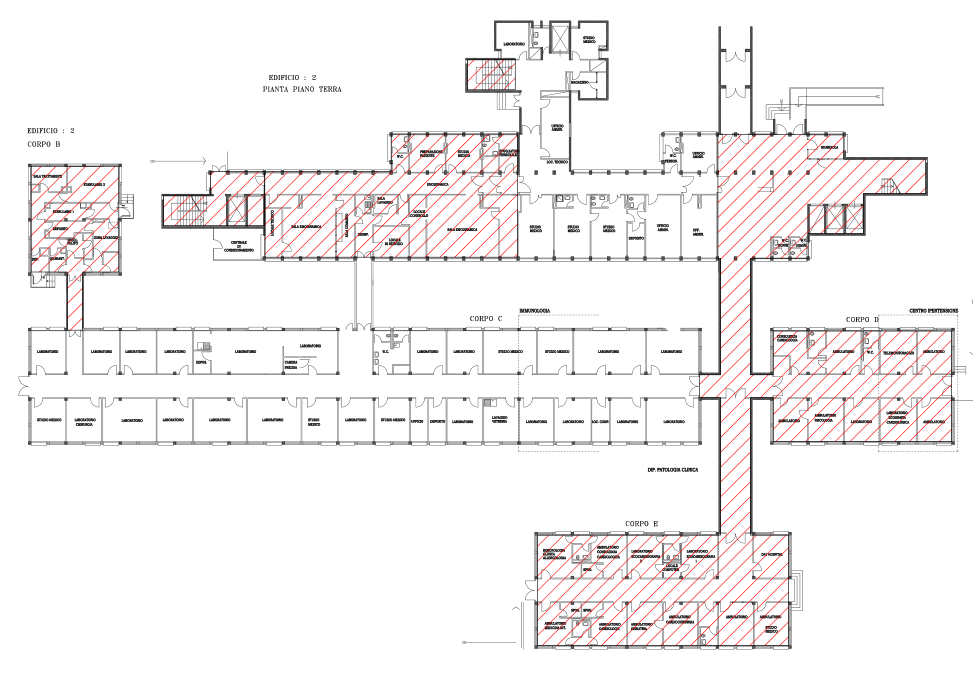
\includegraphics[width=\hsize]{6_2_cap/img/PT}
		\caption{Planimetria Piano Terra -- Edificio 2}
		\label{img:PT}
\end{sidewaysfigure}
\begin{sidewaysfigure}
	\centering
		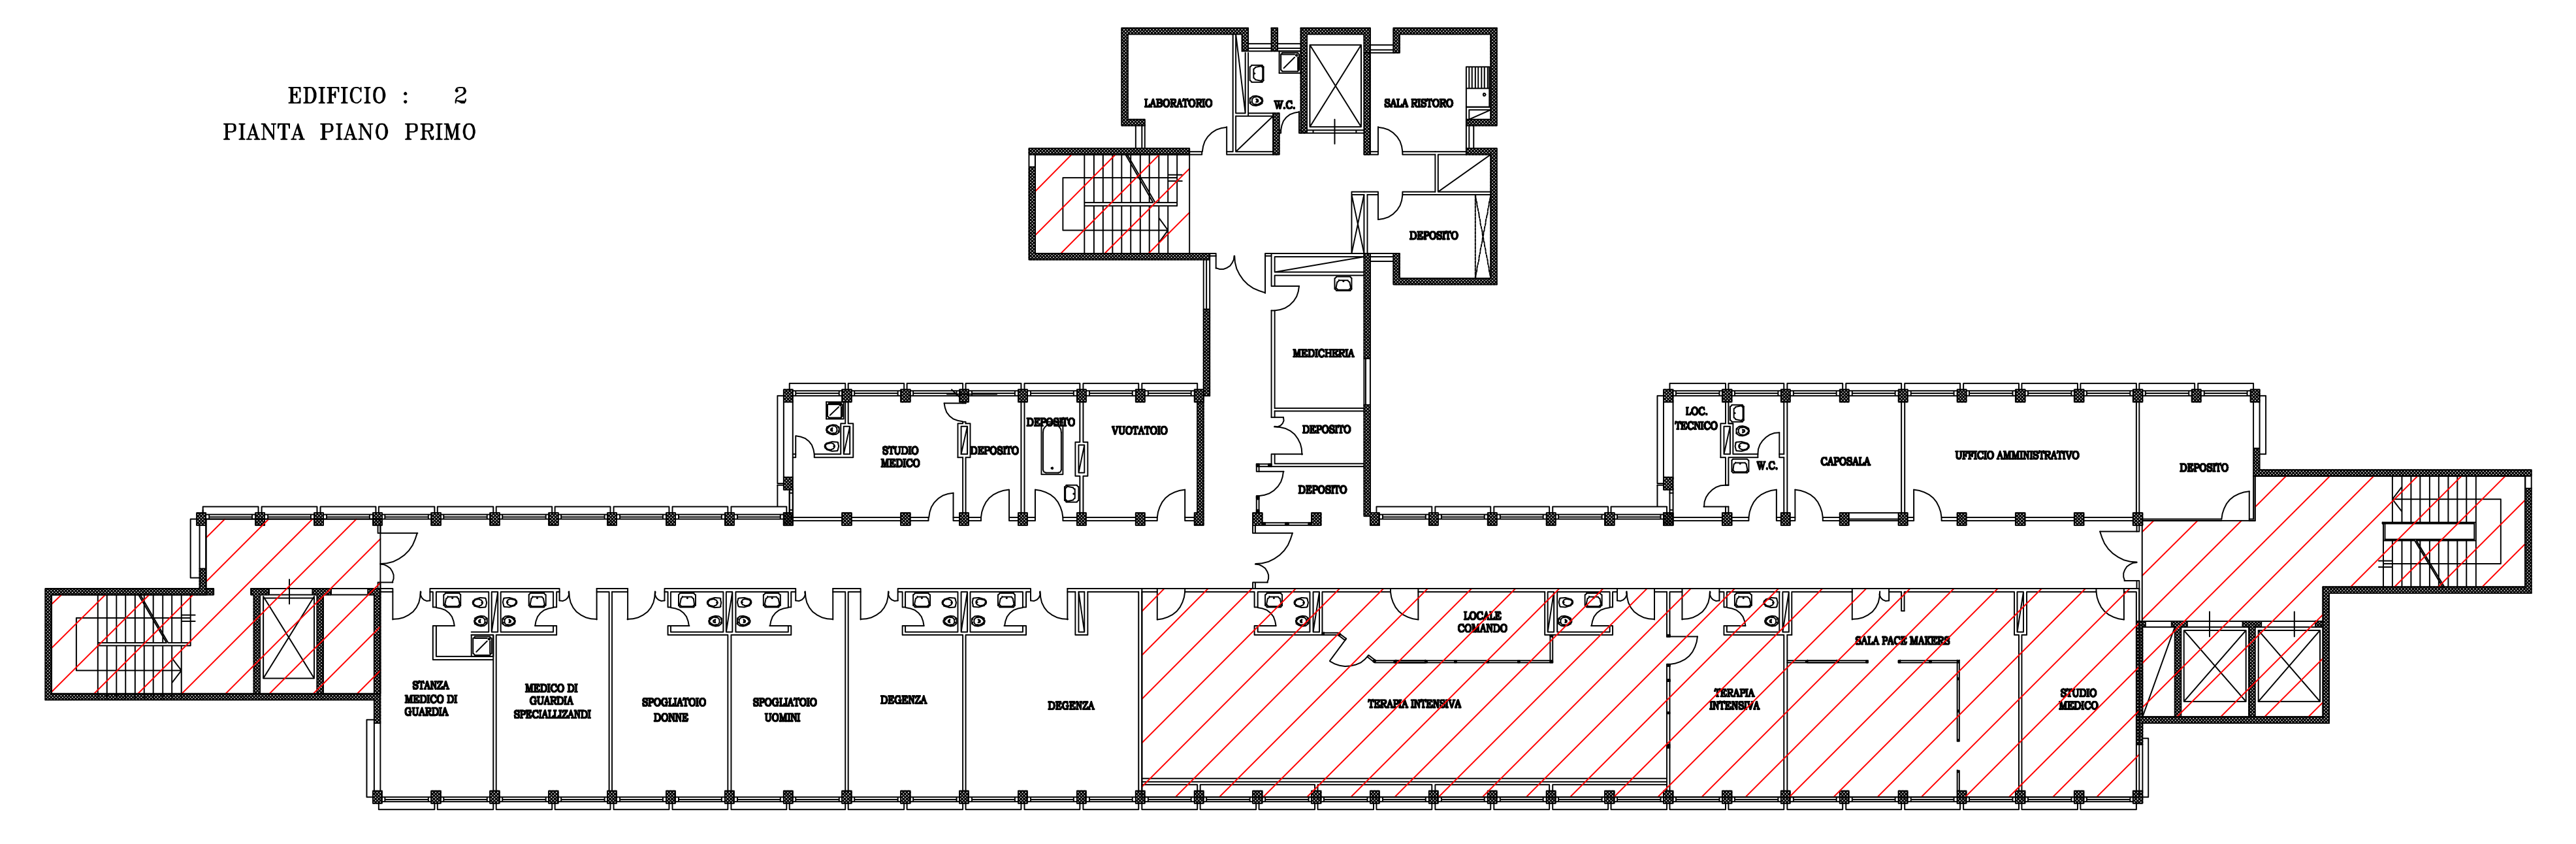
\includegraphics[width=\hsize]{6_2_cap/img/P1}
			\caption{Planimetria Piano Primo -- Corpo A}
			\label{img:P1}
\end{sidewaysfigure}
\begin{sidewaysfigure}
	\centering
	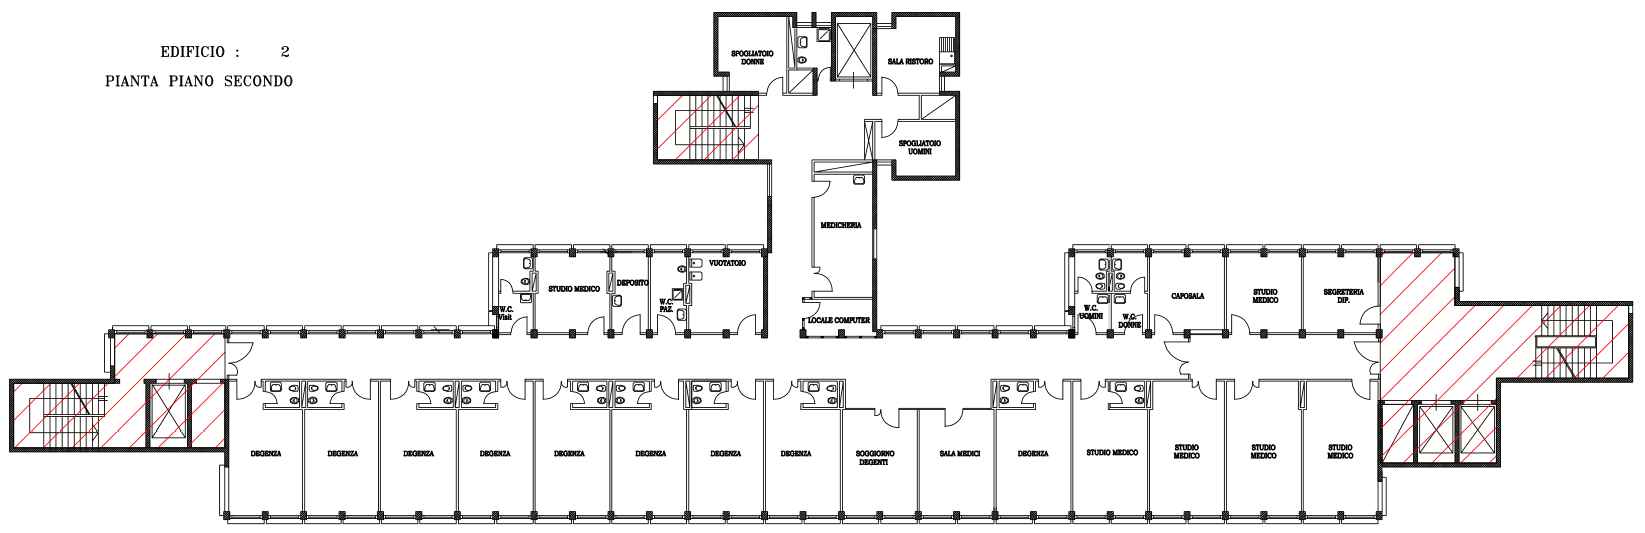
\includegraphics[width=\hsize]{6_2_cap/img/P2}
	\caption{Planimetria Piano Secondo -- Corpo A}
	\label{img:P2}
\end{sidewaysfigure}
\begin{sidewaysfigure}
	\centering
	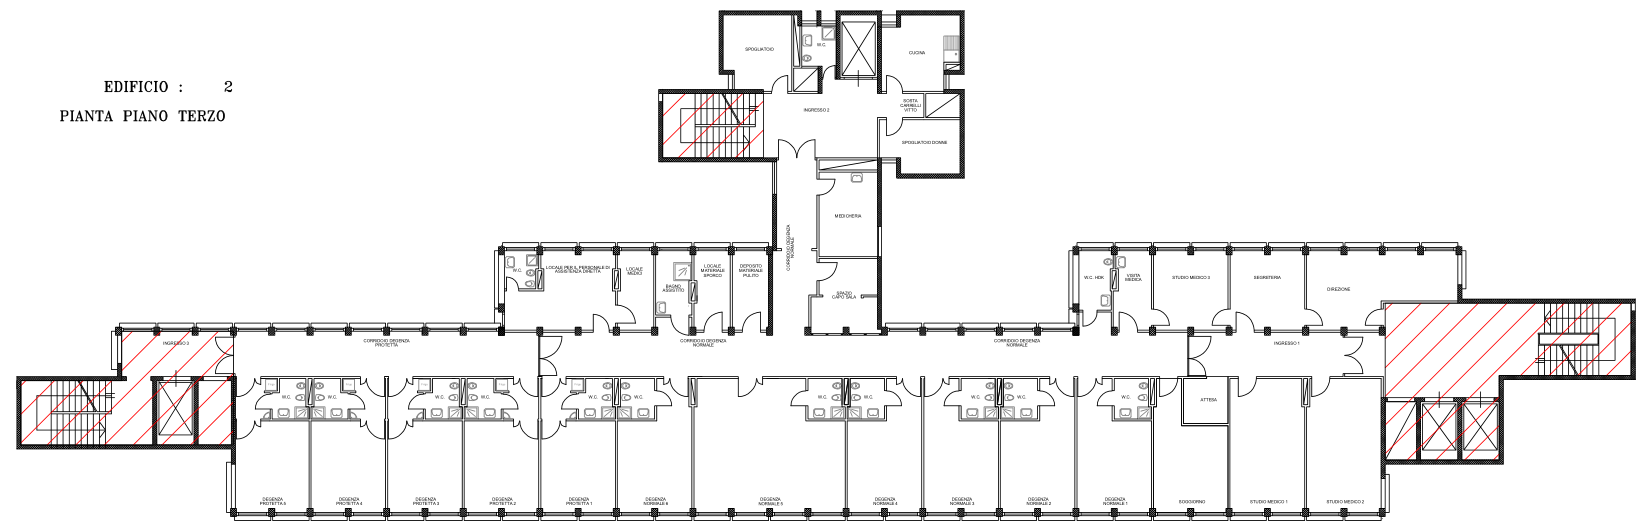
\includegraphics[width=\hsize]{6_2_cap/img/P3}
	\caption{Planimetria Piano Terzo -- Corpo A}
	\label{img:P3}
\end{sidewaysfigure}
\begin{sidewaysfigure}
	\centering
	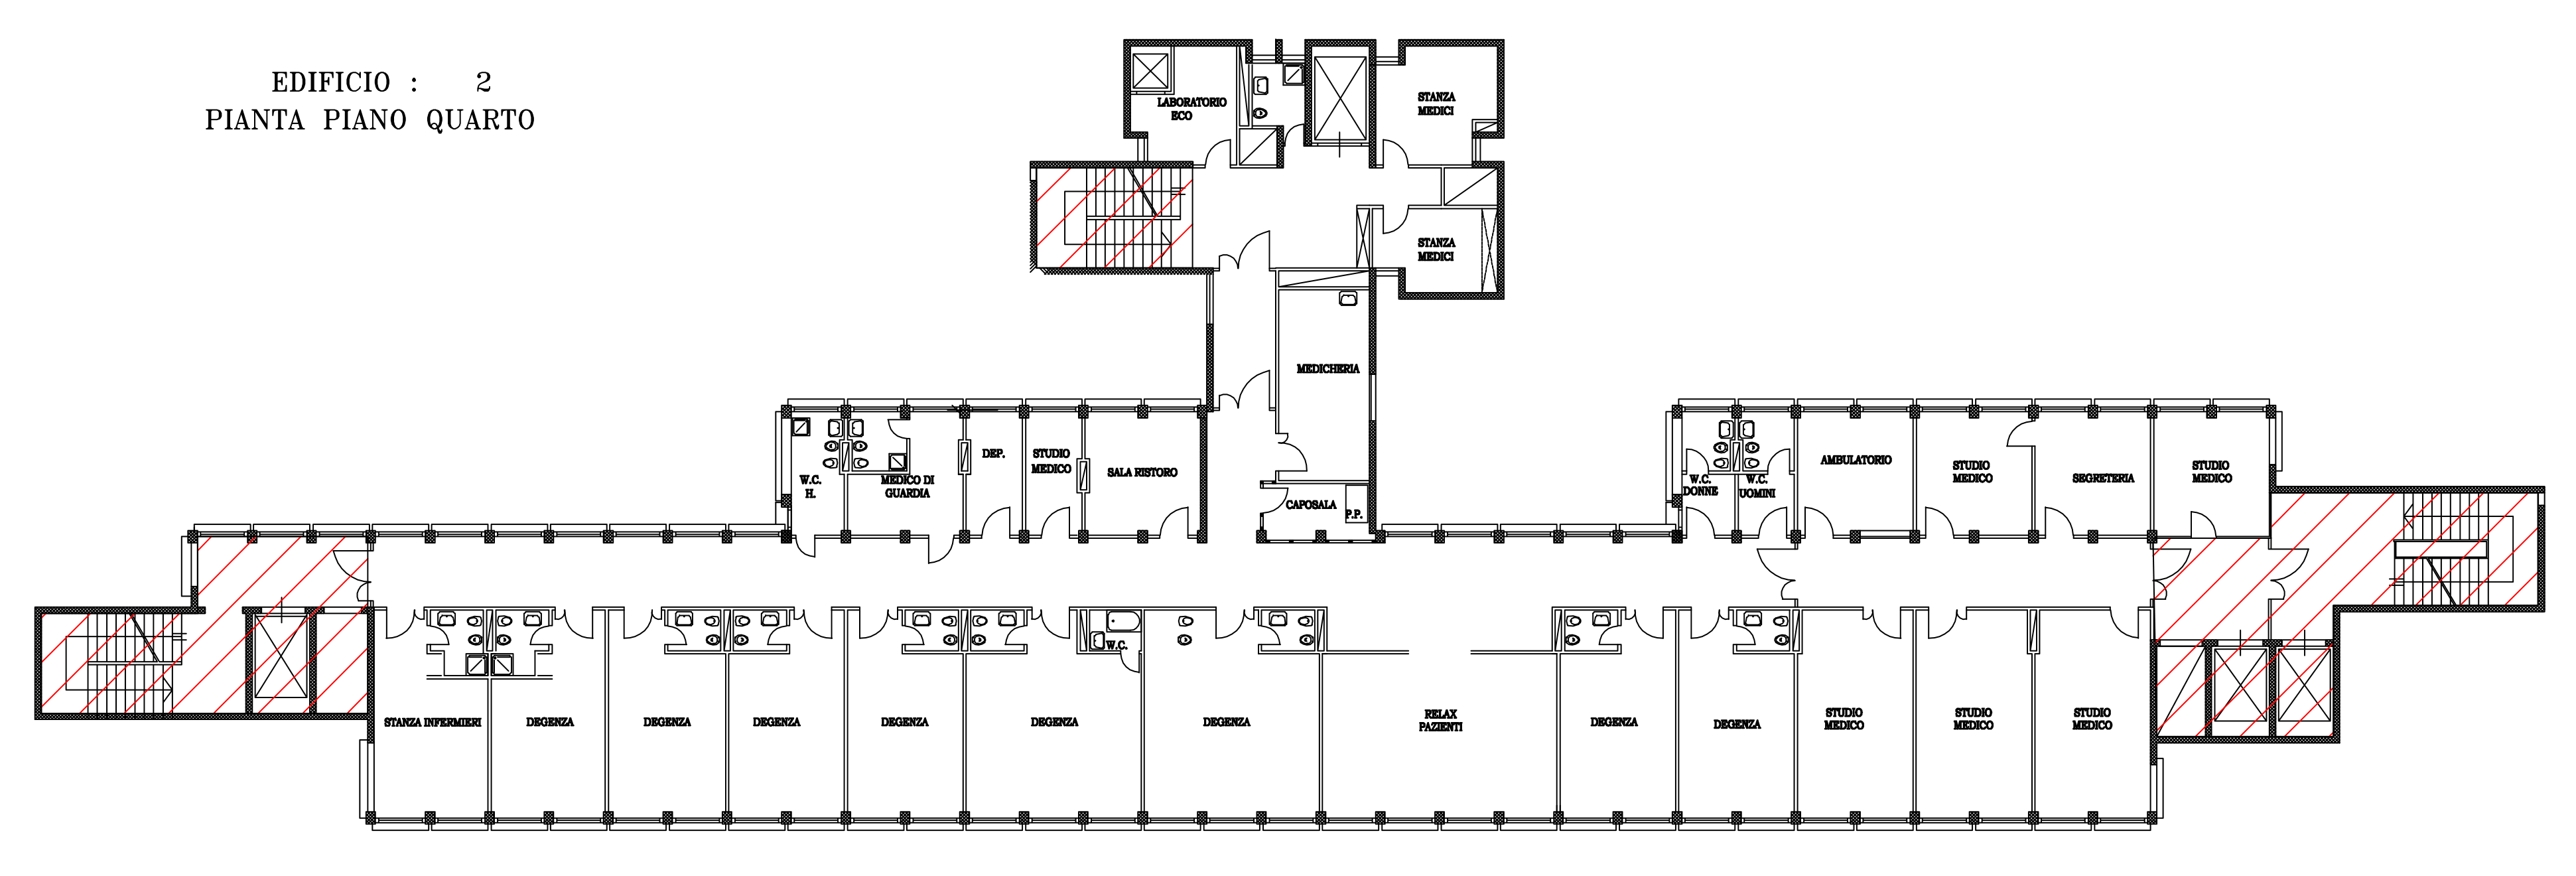
\includegraphics[width=\hsize]{6_2_cap/img/P4}
	\caption{Planimetria Piano Quarto -- Corpo A}
	\label{img:P4}
\end{sidewaysfigure}

%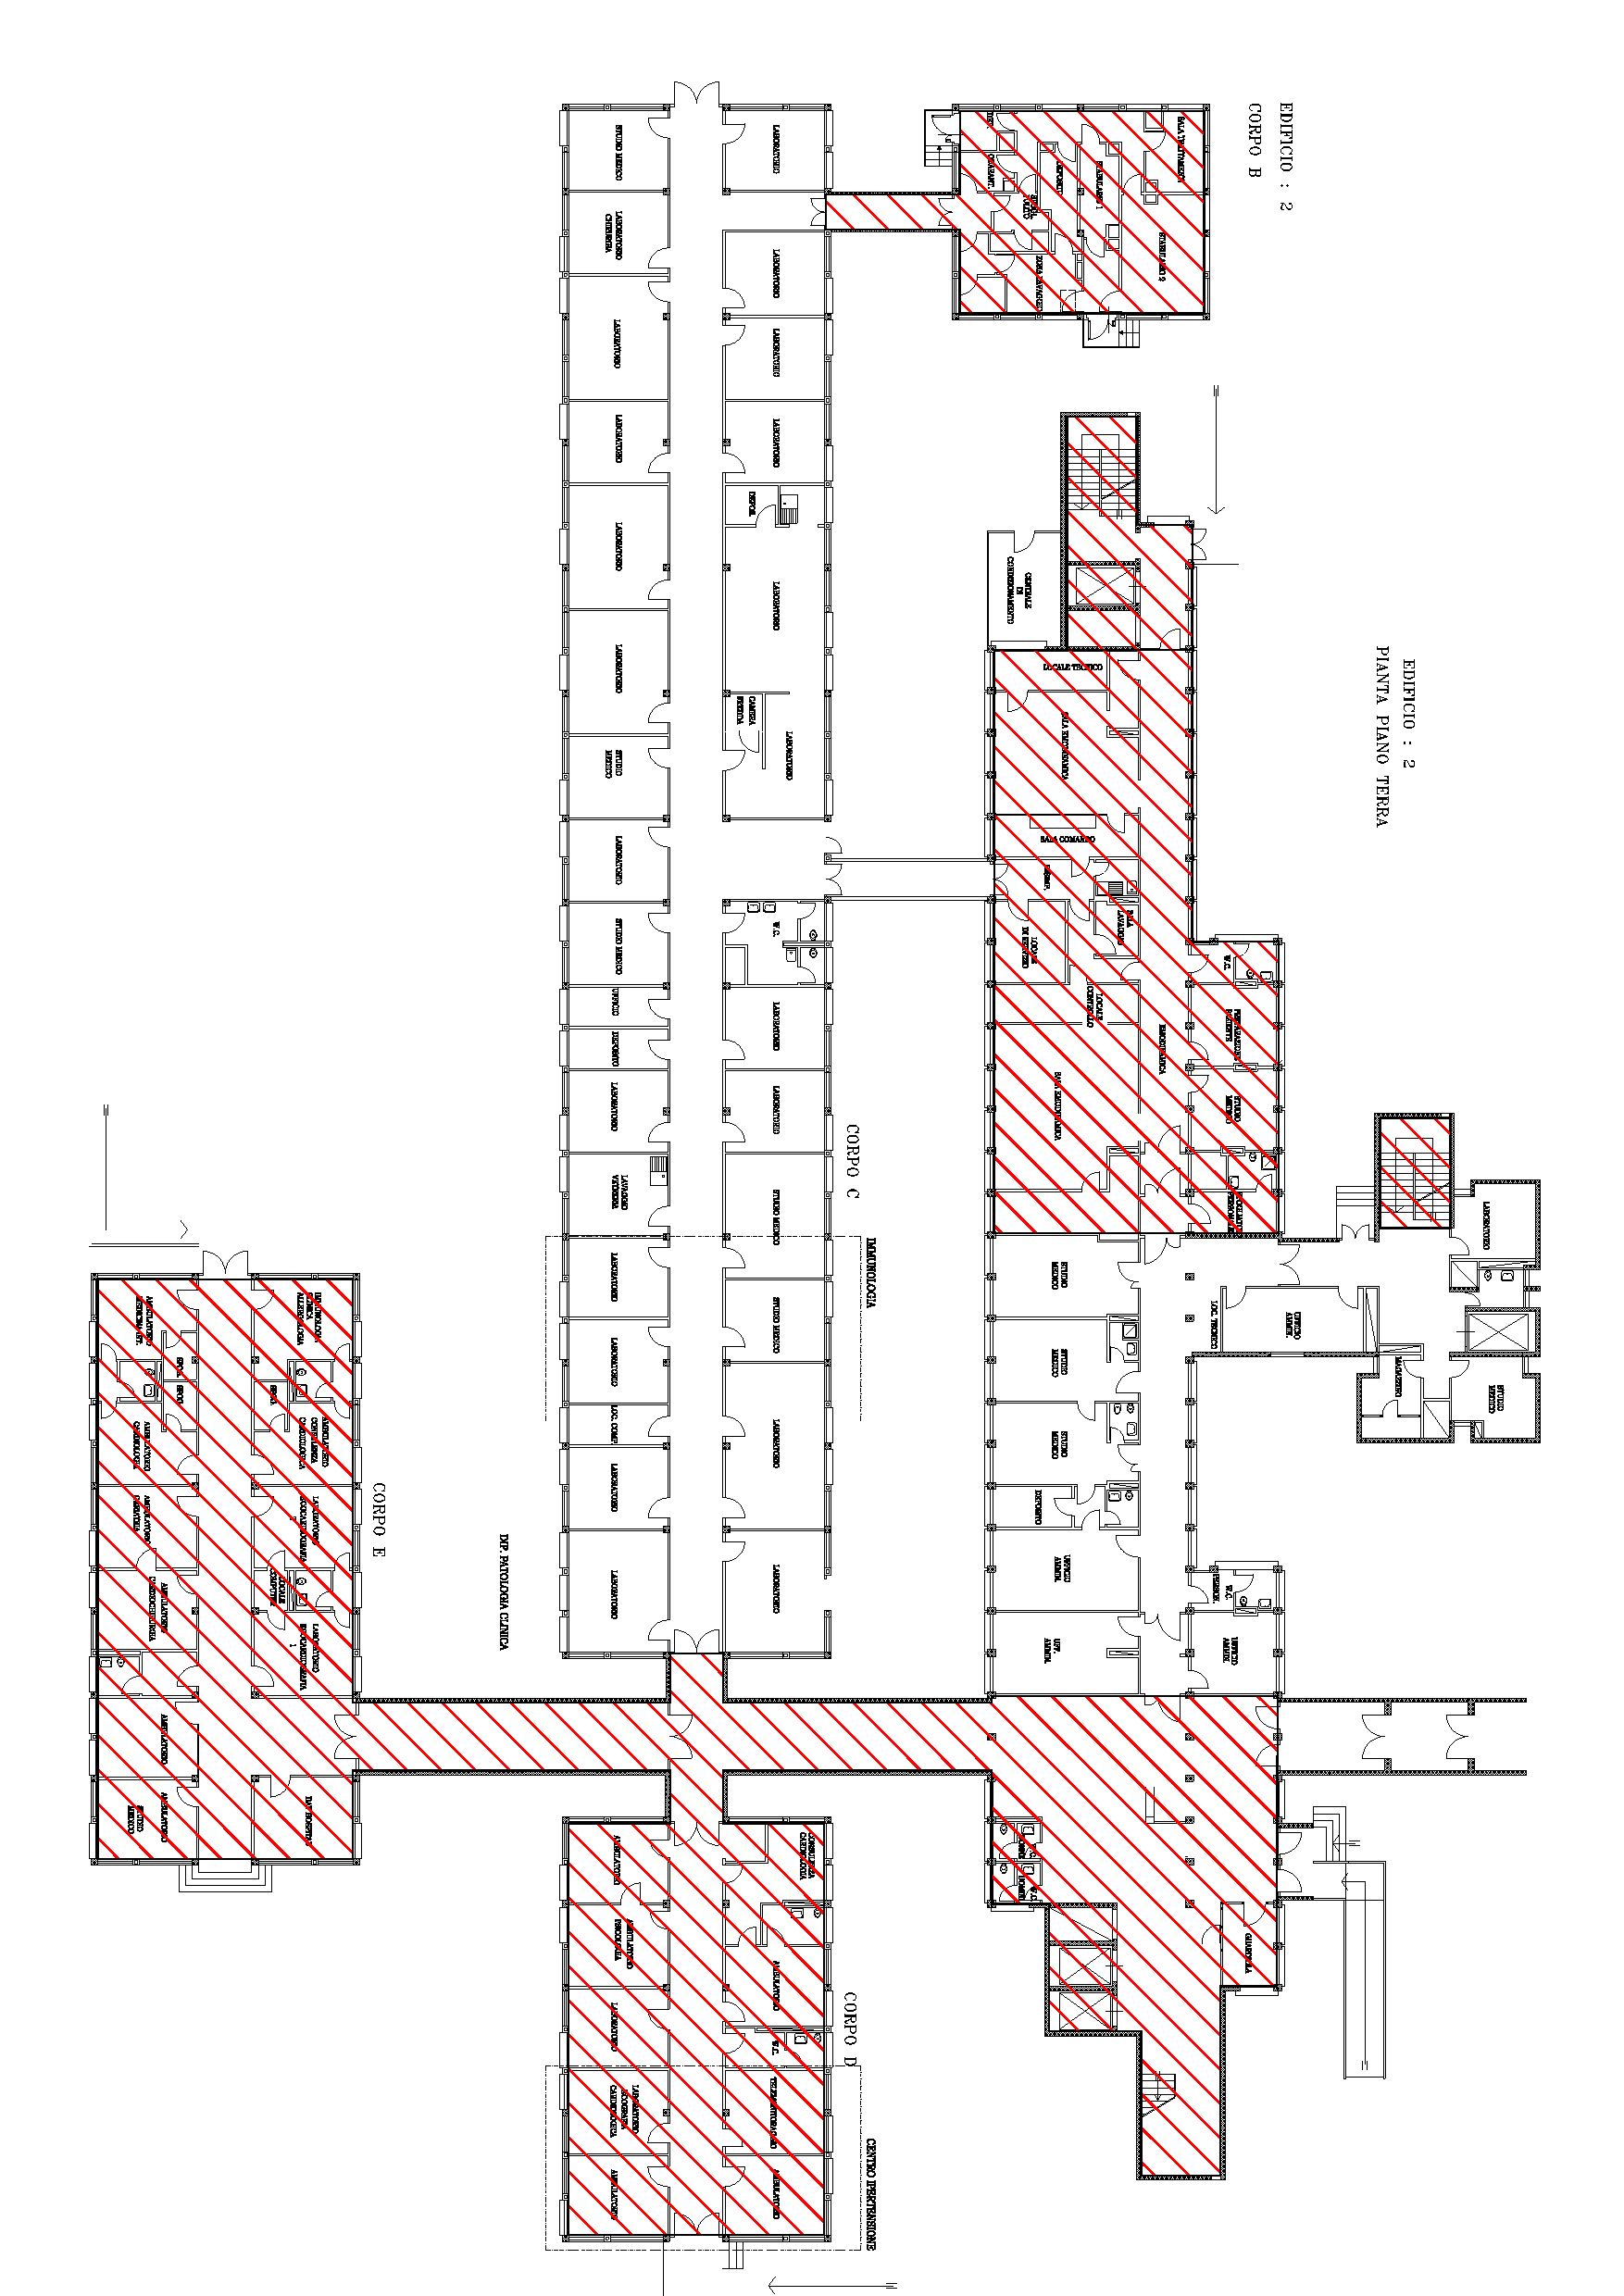
\includepdf{6_2_cap/img/PT.pdf}\label{PT}
%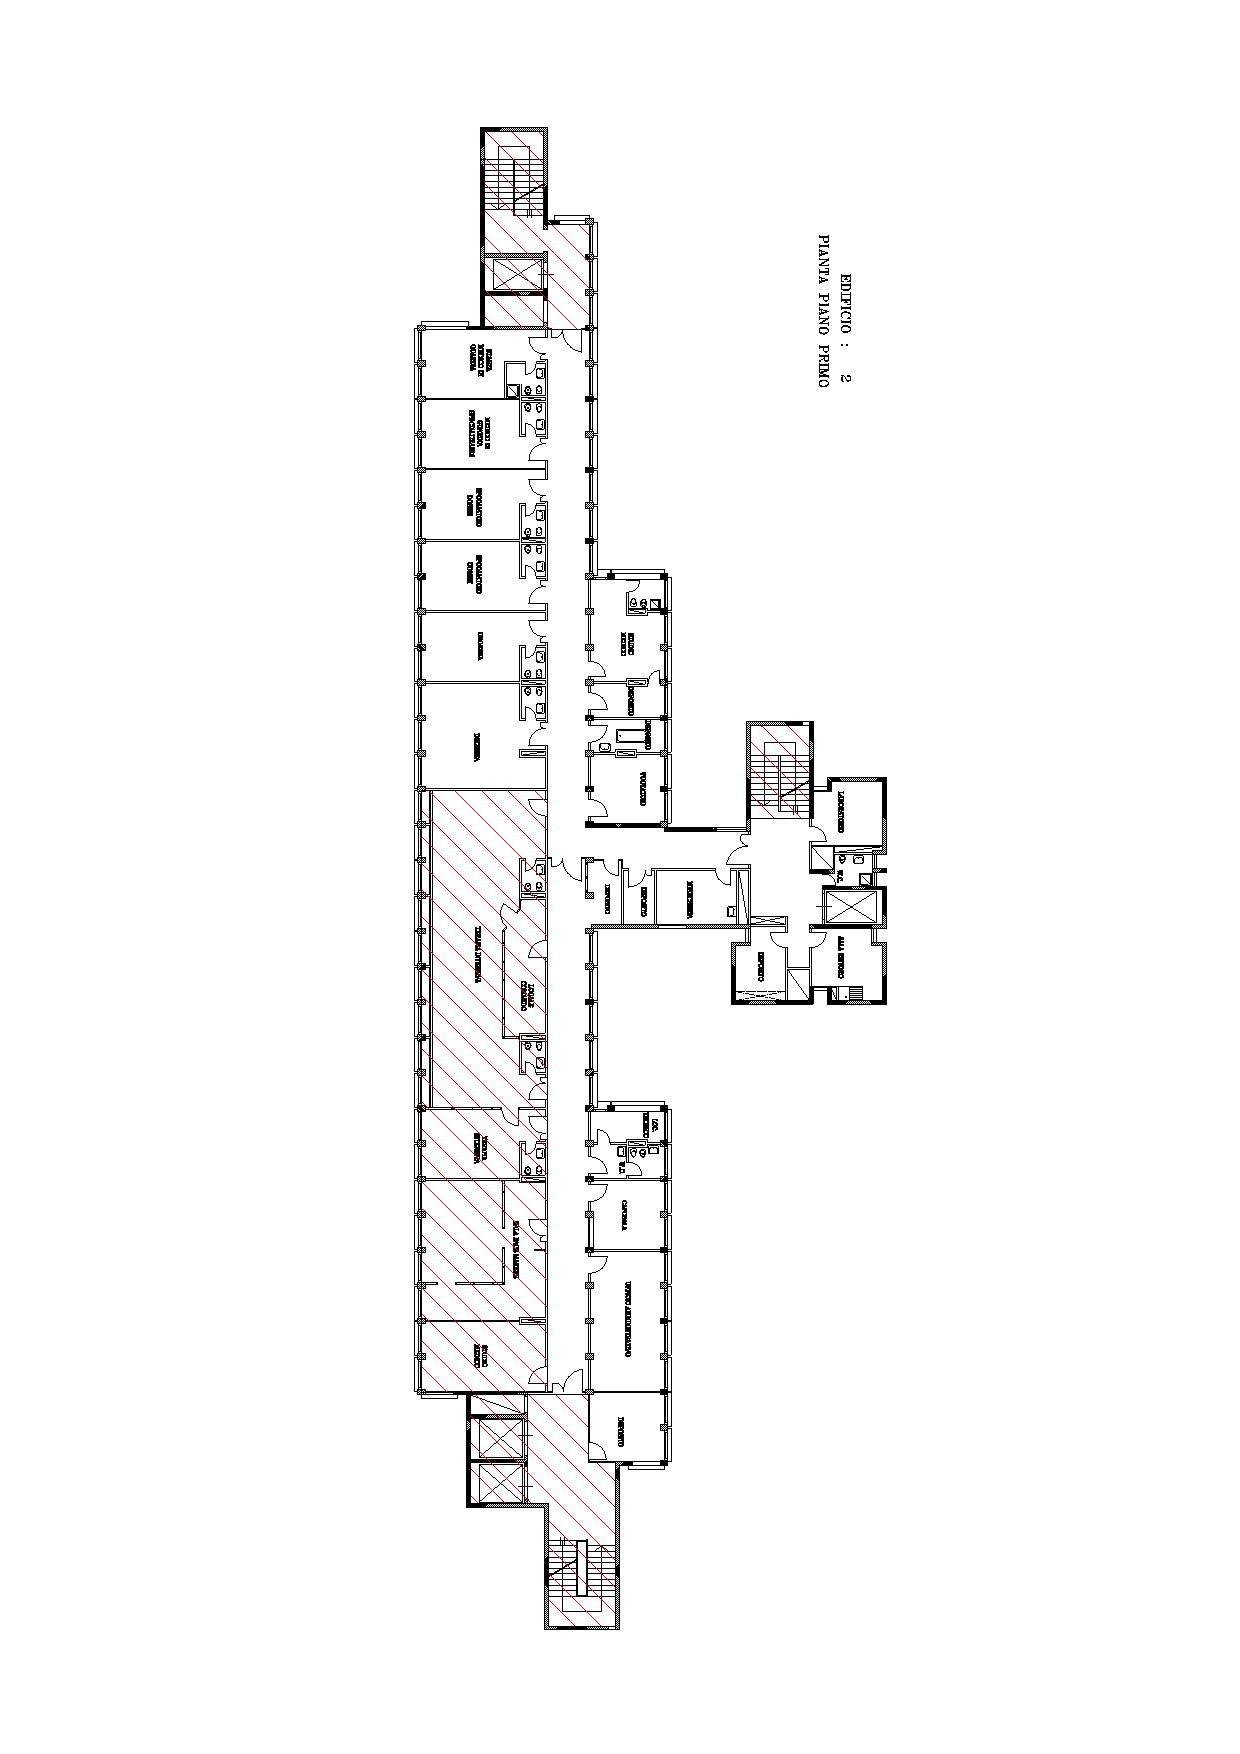
\includepdf{6_2_cap/img/P1.pdf}\label{P1}
%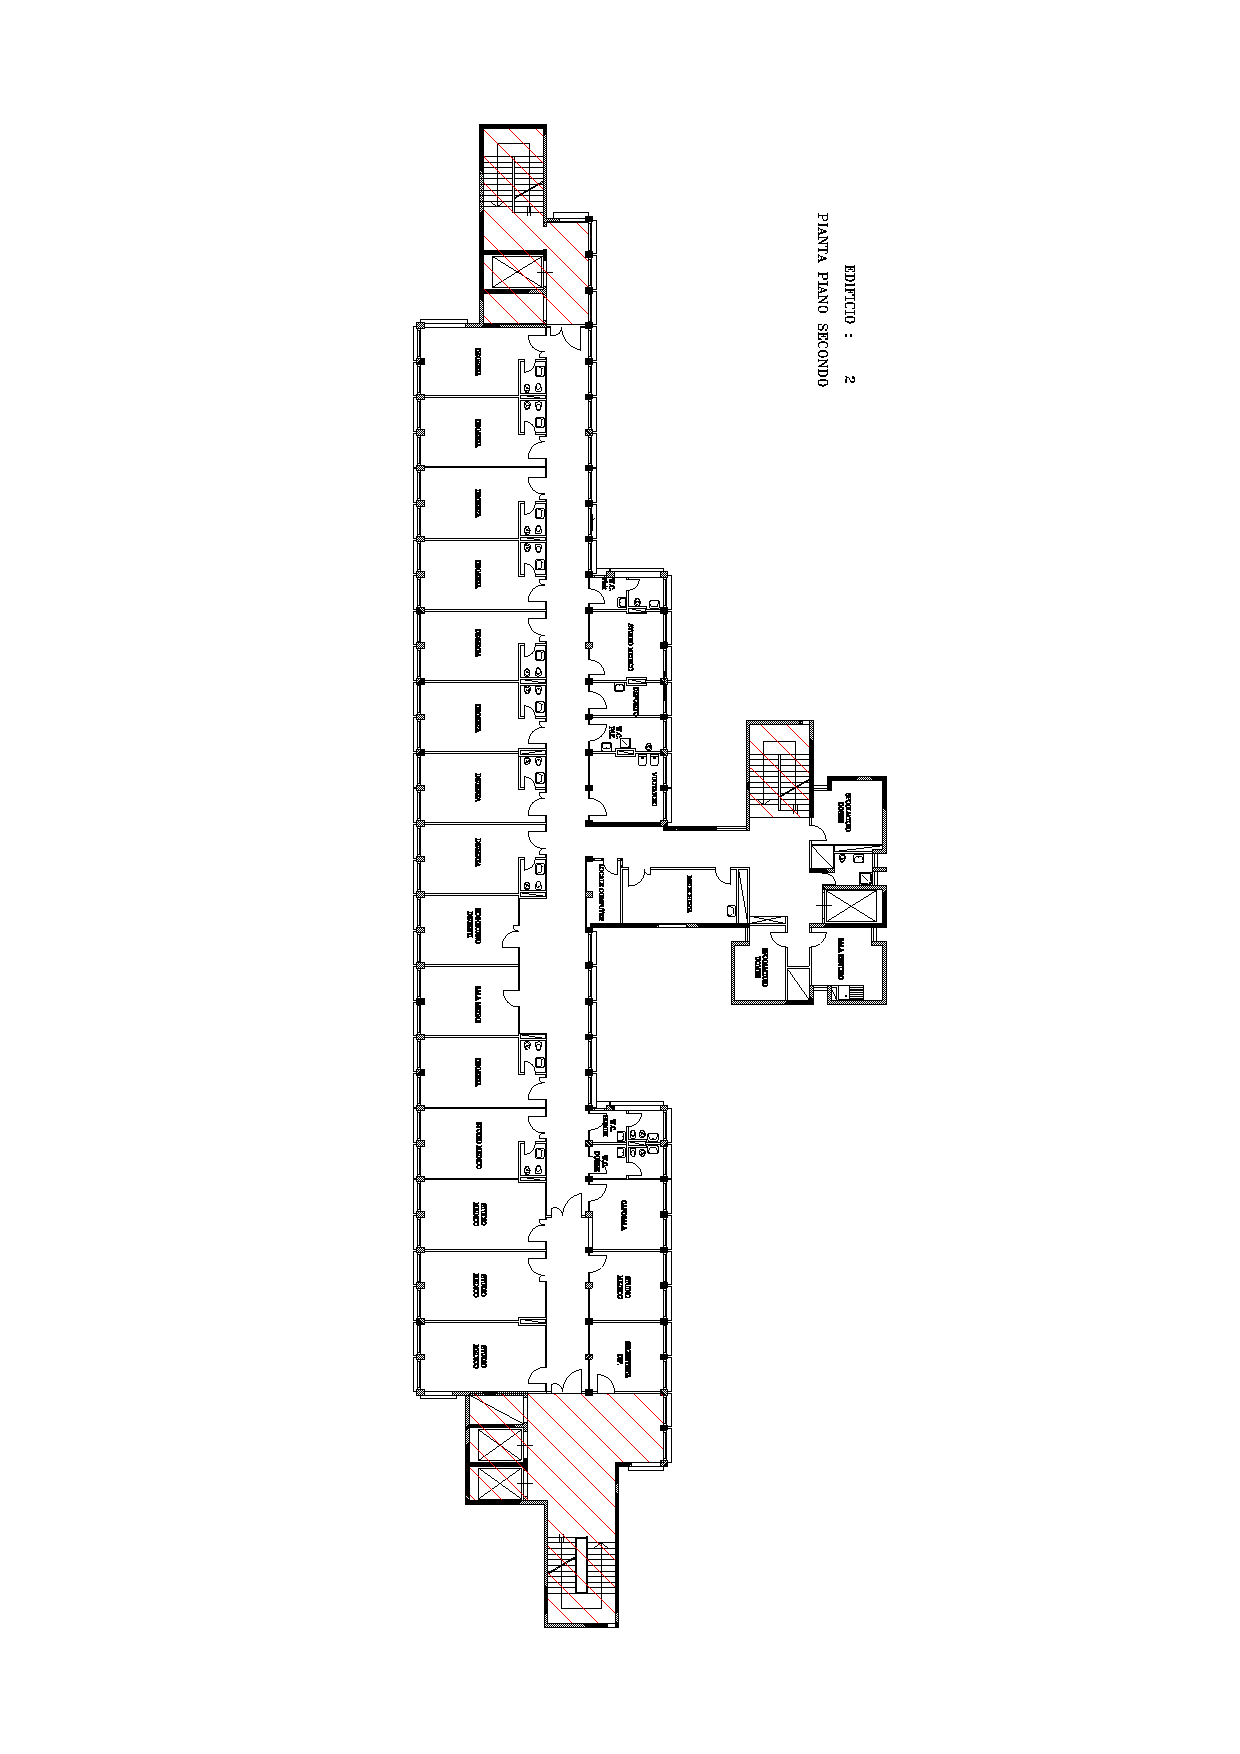
\includepdf{6_2_cap/img/P2.pdf}\label{P2}
%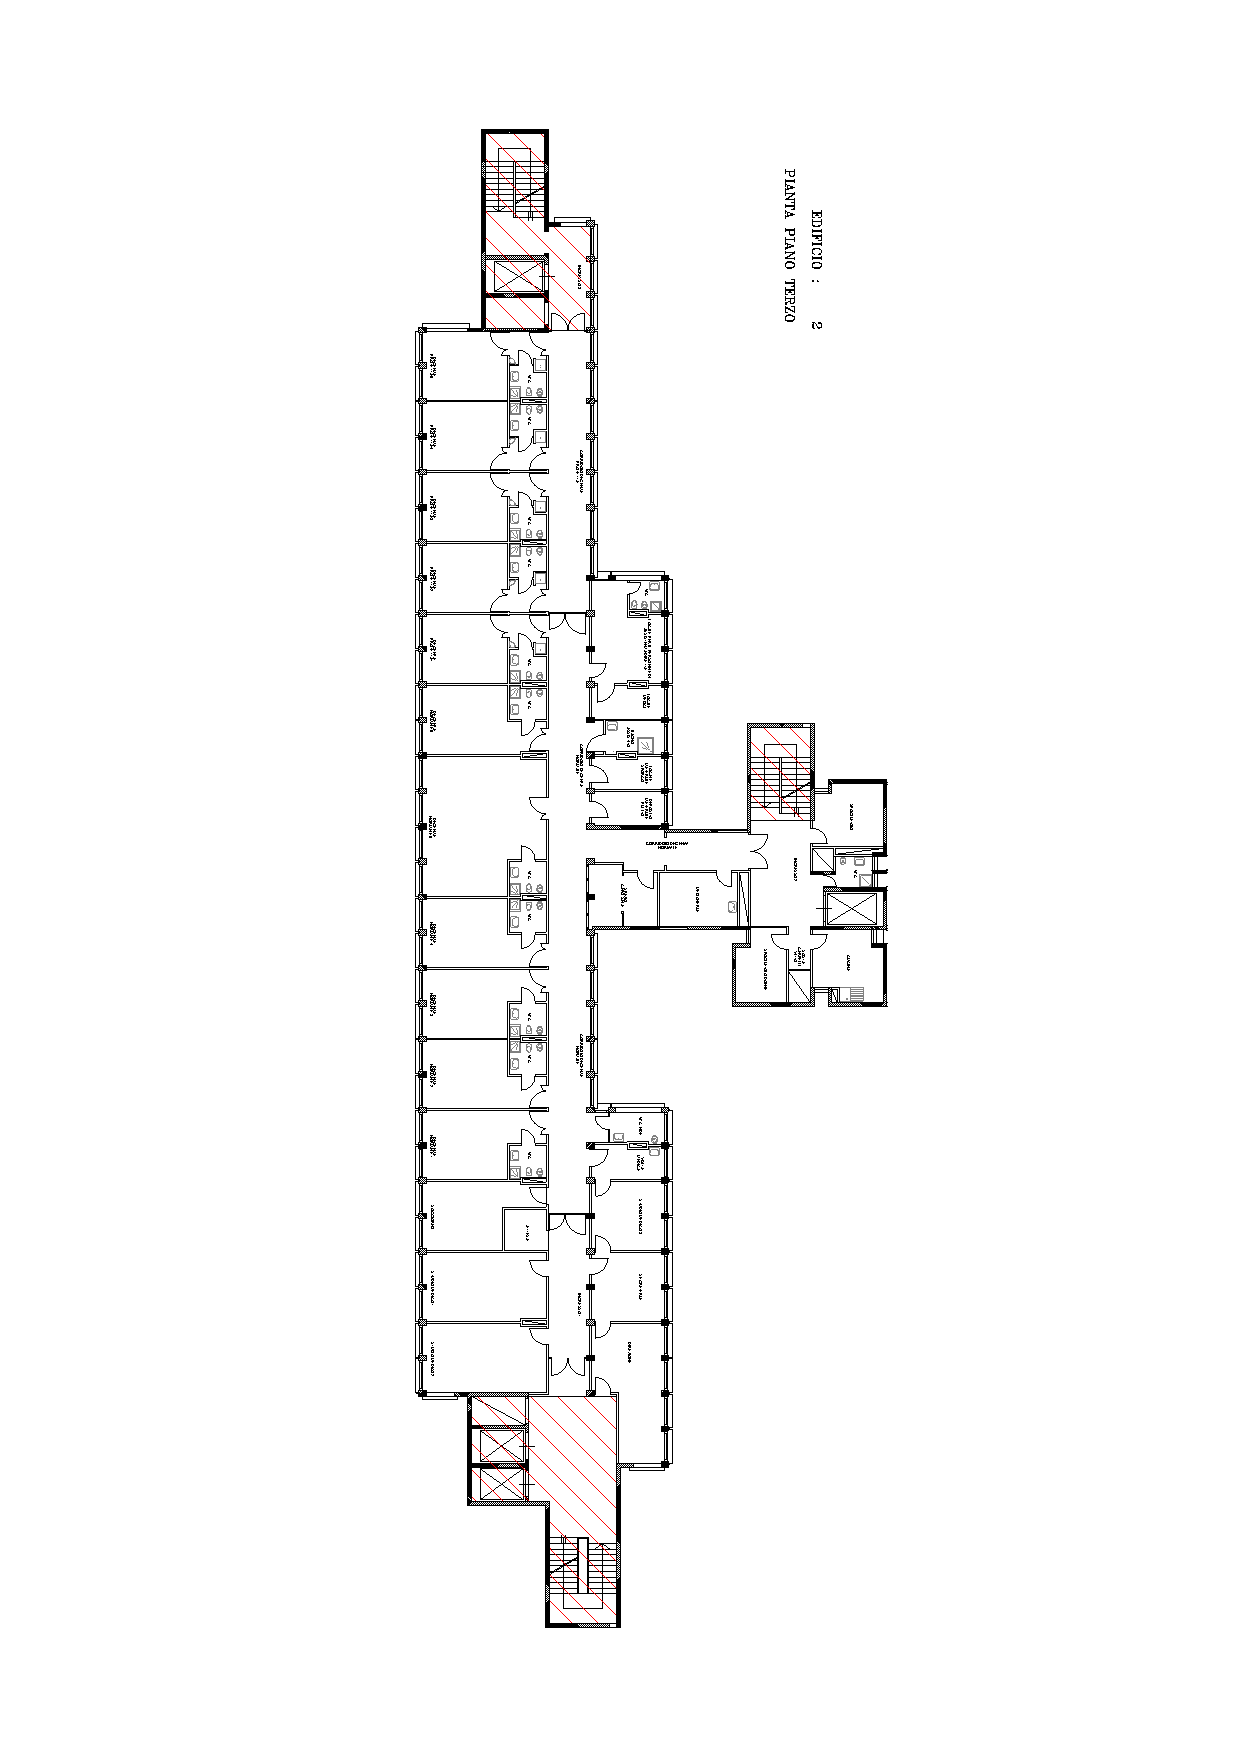
\includepdf{6_2_cap/img/P3.pdf}\label{P3}
%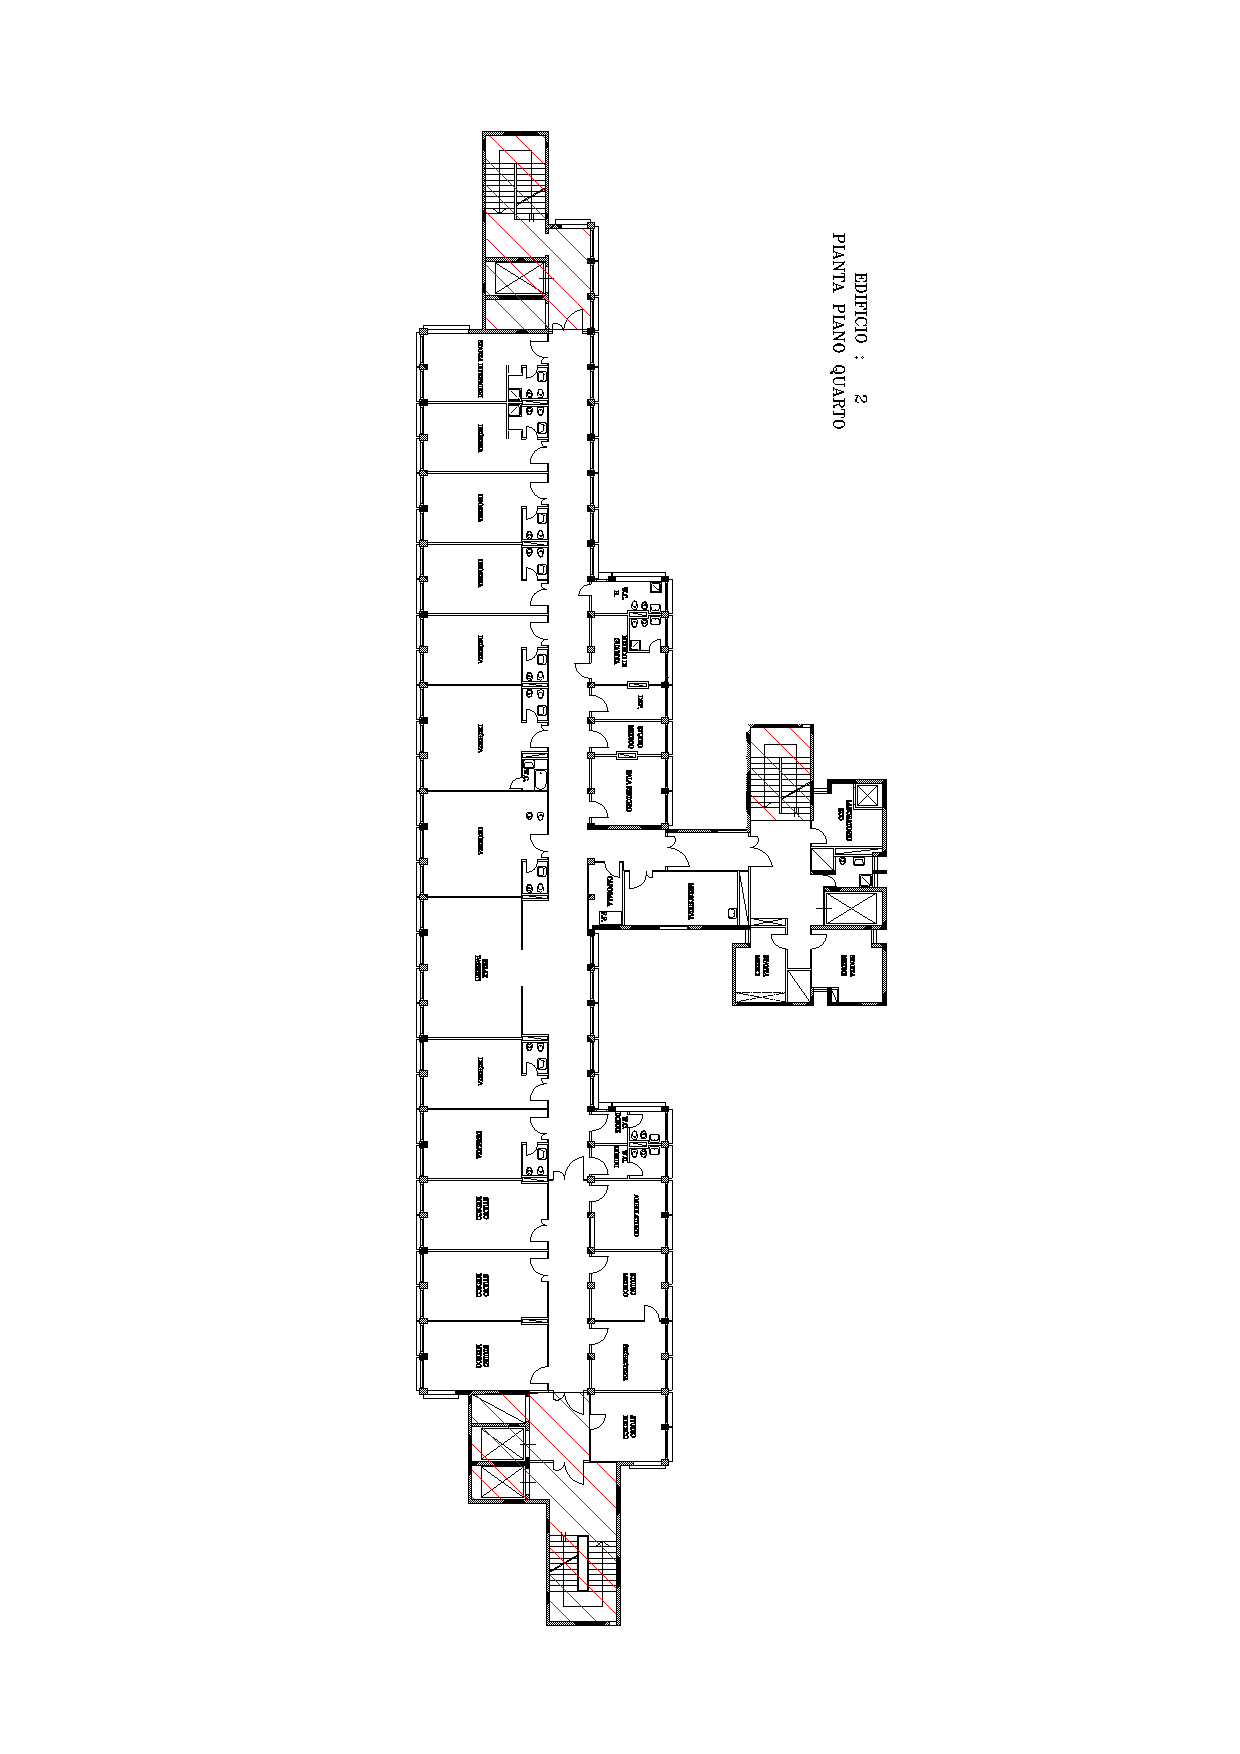
\includepdf{6_2_cap/img/P4.pdf}\label{P4}
\clearpage
\section{I risultati energetici}
\begin{figure}[p]
	\centering
	\subfloat[][Radiatori]{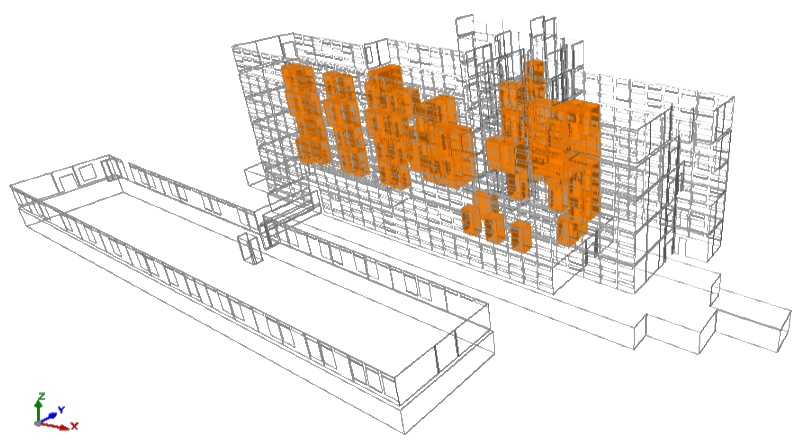
\includegraphics[width=0.45\textwidth]{6_2_cap/img/rad}\label{rad}}\quad
	\subfloat[][V Piano]{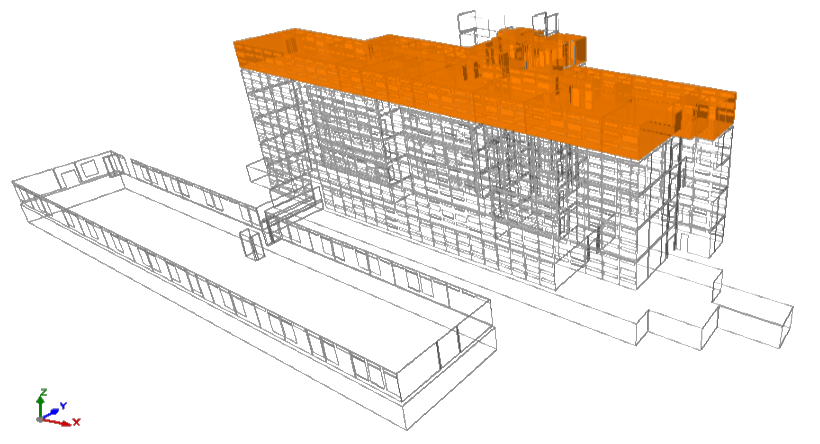
\includegraphics[width=0.45\textwidth]{6_2_cap/img/vpiano}\label{vpiano}}\\
	\subfloat[][Emodinamica]{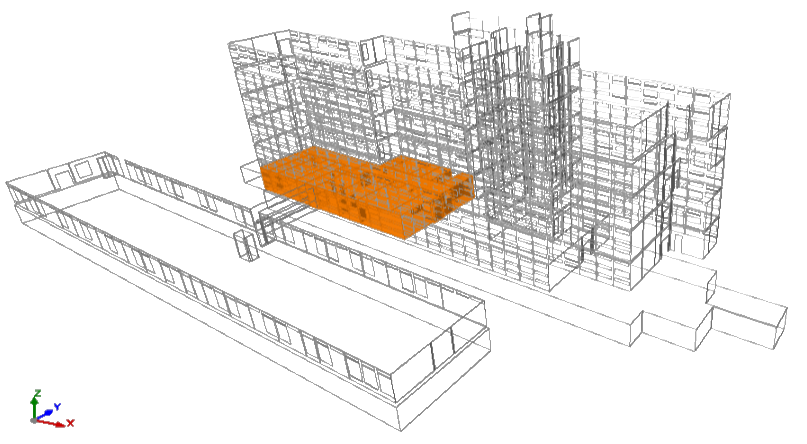
\includegraphics[width=0.45\textwidth]{6_2_cap/img/emo}\label{emo}}\quad
	\subfloat[][UTIC]{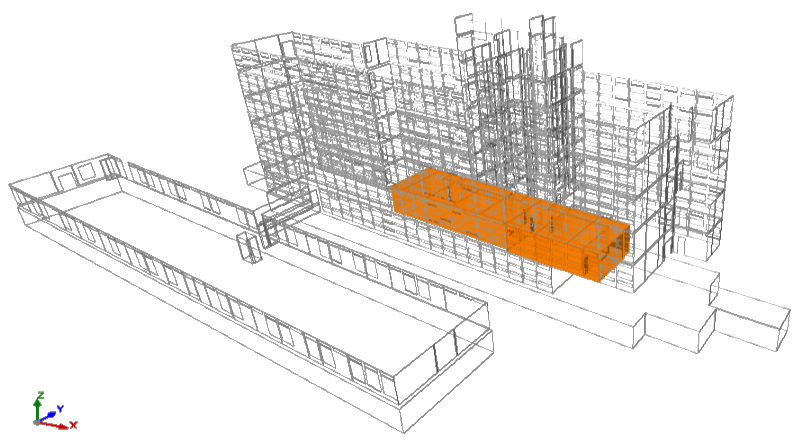
\includegraphics[width=0.45\textwidth]{6_2_cap/img/utic}\label{utic}}\\
	\subfloat[][Corpo A]{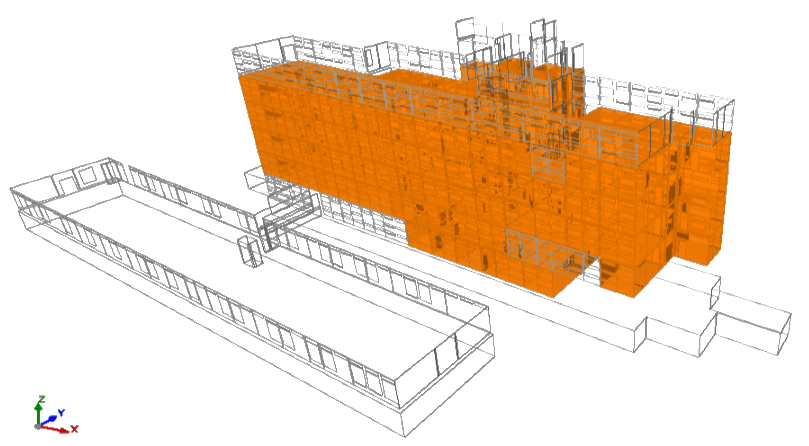
\includegraphics[width=0.45\textwidth]{6_2_cap/img/ca}\label{ca}}\quad
	\subfloat[][Corpo C]{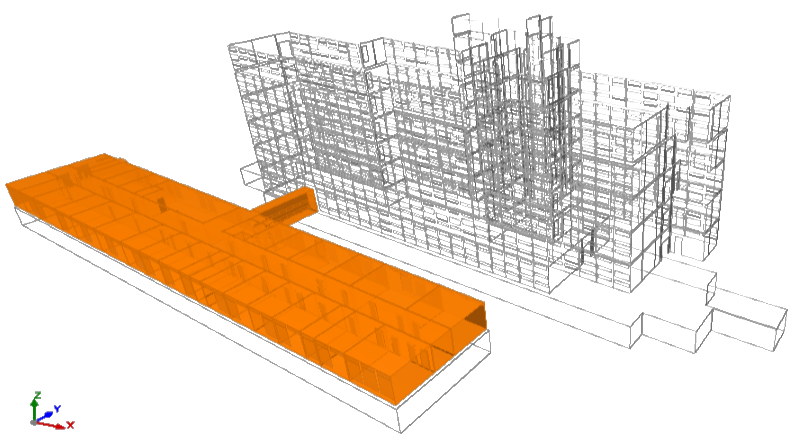
\includegraphics[width=0.45\textwidth]{6_2_cap/img/cb}\label{cb}}
	\caption{Le zone termiche}\label{zt}
\end{figure}

L'edificio è stato suddiviso in 5 zone termiche visualizzabili in \vref{zt}:
\begin{itemize}
	\item \textbf{V Piano};
	\item \textbf{UTIC};
	\item \textbf{Emodinamica};
	\item \textbf{Corpo A} (escluse le zone del V Piano, UTIC e Emodinamica);
	\item \textbf{Corpo C};
	\item \textbf{Radiatori}: ovvero tutti i servizi igienici del Corpo A. 
\end{itemize}
È necessario spiegare il motivo di questa suddivisione.

Innanzitutto le prime tre zone termiche sono state separate dal resto del Corpo A in quanto il loro impianto non è oggetto di intervento ma è comunque interessante conoscere il risparmio in potenza che si riesce ad ottenere modificando l'involucro.

Per quanto riguarda la zona \emph{Radiatori}, è effettivamente sbagliato dal punto di vista termico considerarla esclusa dal resto del Corpo A in quanto non sono due zone termiche distinte. Questa forzatura è stata necessaria in quanto dai risultati ottenuti non era possibile scindere i carichi sensibili dei servizi igienici dal resto dell'edificio. Siccome i radiatori verranno posizionati solo nei servizi igienici, era interessante conoscere, quindi, il carico termico dei soli servizi igienici per poi dimensionare adeguatamente l'impianto a suo servizio. 

\subsection{Stagione Estiva}
Si presentano i vari risultati ottenuti con la dovuta teoria che vi è alla base.

Nel secondo capitolo si è già abbondantemente spiegato il motivo per cui è necessario considerare anche i carichi interni e quelli latenti.

Le valutazioni energetiche sono state effettuate con una temperatura e umidità esterna rispettivamente di \n{35}{\degreeCelsius} con il \n{60}{\%} maggiore di quella consigliata dalla \norvent\ per la città di Napoli. All'interno, invece, si sono rispettate le condizioni di benessere termo-igrometrico: \n{24}{\degreeCelsius} con il \n{50}{\%}. Per la ventilazione si è proceduto considerando per ogni locale i ricambi orari minimi.

Relativamente ai soli reparti di Emodinamica, UTIC e Blocco Operatorio che possiedono un loro impianto dedicato a \emph{tutt'aria} si è proceduto in questo modo:
sono note le superfici e le altezze dei vari locali come anche il carico esterno solare e di trasmissione; si sono supposti i \num{10} ricambi orari di aria esterna (per le sale chirurgiche e di terapia intensiva del blocco operatorio si sono fissati i \num{20} ricambi orari arrivando a \num{11} ricambi medi su tutto il piano); un affollamento di $n=\SI{0.08}{pers/m^2}$; un carico sensibile e latente per le persone pari rispettivamente a $Q_{\mathrm{pers,S}}=\SI{70}{W/pers}$ e $Q_{\mathrm{pers,L}}=\SI{50}{W/pers}$; un carico interno per le varie apparecchiature di $Q_{\mathrm{int,S}}=\SI{10}{W/m^2}$. 

Nella seguente tabella sono mostrati i parametri di input e i risultati per le 3 zone termiche considerate.
\begin{center}
	\begin{tabular}{lccccc}
		\toprule
					&	Superficie 				&	Portata Aria Est. 			&	$\dot{Q}_{\mathrm{sol}}+\dot{Q}_{\mathrm{trasm}}$		& 	\multirow{2}{*}{RST}		&	$\dot{Q}_{\mathrm{frigo}}$ 	\\
					&	{\small \si{m^2}}		&		{\small \si{kg/s}}		&		{\small \si{kW}}				&								&{\small \si{kW}}		\\					
		\midrule	
		UTIC		&		\num{146}			&		\num{1.46}				&	\num{7.62}		&	0.94					&	\num{10.5}		\\
		Emod.		&		\num{169}			&		\num{1.69}				&	\num{13.2}		&	0.96					&	\num{16.5}		\\
		B.O.		&	\num{697}				&		\num{7.33}				&	\num{34.6}		&	0.94					&	\num{48.3}		\\
		\bottomrule
	\end{tabular}
\end{center}
RST sta per \emph{Rapporto Sensibile su Totale} ed è adimensionale. È molto importante nei diagrammi psicrometrici in quanto permette di individuare i luoghi dei punti di immissione dell'aria (nel caso di impianti a tutt'aria o di miscelazione in quelli misti) che bilanciano adeguatamente sia il carico sensibile che latente. Siccome nel nostro caso il suo valore è prossimo all'unità avremo un carico da bilanciare che è pressoché tutto sensibile.

Conoscendo il valore di RST, del carico da bilanciare $Q_{frigo}$ e della portata di ventilazione, dal diagramma psicrometrico si individuano, per ogni zona termica (e le loro rispettive UTA), le proprietà termoigrometriche dell'aria da immettere. Ed è, quindi, possibile calcolare le potenze delle batterie di raffreddamento e post-riscaldamento delle UTA nel caso estivo. Nella seguente tabella sono riassunti i risultati ottenuti in \si{kW}. L'ipotesi alla base di tutte queste valutazioni è che le batterie siano ideali cioè che non vi sia una frazione di portata d'aria che non entri a contatto con le lamelle delle batterie stesse. In questa sede, però, volendo solo effettuare una valutazione pre e post intervento non è importante considerare anche il cosiddetto \emph{by-pass factor} delle batterie (anche se oggigiorno suddetti fattori risultano essere dell'ordine del \n{5}{\%} e quindi tranquillamente trascurabili).
\begin{center}
	\begin{tabular}{lcc}
		&	$\dot{Q}_{\mathrm{UTA,f}}$		&	$\dot{Q}_{\mathrm{UTA,c}}$\\
		\midrule
		UTIC	&	\num{79.3}			&	\num{6.86}\\
		Emod.	&	\num{91.7}			&	\num{3.52}\\
		B.O.	&	\num{664}			&	\num{39.0}\\
	\end{tabular}
\end{center}
La potenza di raffreddamento e riscaldamento viene fornita da una opportuna portata d'acqua prodotta in sottocentrale. Una rapida valutazione delle portate in gioco, restituisce i valori, in \si{l/s}, riportati nella tabella successiva. Per questioni tecnologiche le temperature di mandata e ritorno dell'acqua sono rispettivamente di \num{7} e \n{12}{\degreeCelsius} per la batteria di raffreddamento mentre di \num{60} e \n{55}{\degreeCelsius} per quelle di riscaldamento e che il calore specifico dell'acqua è ritenuto costante e pari a $c_p=\SI{4.2}{kJ/kgK}$.
\begin{center}
	\begin{tabular}{lcc}
			&	$\dot{m}_f$	&	$\dot{m}_c$\\
			\midrule
			UTIC	&	\num{3.8}	&	\num{0.33}\\
			Emod.	&	\num{4.4}	&	\num{0.17}\\
			B.O.	&	\num{32}		&	\num{1.8}\\
	\end{tabular}
\end{center}

Per quanto riguarda \corpa\ e \corpc, l'impianto utilizzato è di tipo \emph{misto} (come nel III e IV piano) o addirittura assente. Pertanto non ne è stata effettuata una valutazione sulla ventilazione ma i risultati considerano solo la trasmissione tramite l'involucro e i carichi interni: apparecchiature e persone.

Per la zona termica \radd\ è ovvio che il carico di raffreddamento sia nullo.

In \vref{stato:fatto} sono riassunti tutti i risultati ottenuti per la stagione estiva nello stato di fatto. 
%{Per i radiatori ovviamente la potenza di raffrescamento è nulla. Per UTIC, BO e EMO il totale tiene conto della trasmissione (ottenuta da CYPE) mentre i carichi interni (sensibili e latenti) sono stati calcolati su Excel. Poi tramite diagramma psicrometrico ho calcolato anche la potenza di ventilazione. Per i corpi A e C i valori del sensibile e del latente non tengono conto della ventilazione.}
\begin{table}
		\centering
		\small
		\begin{tabular}{lccccc}
			\toprule
			\multirow{2}*{Zona Termica} & Superficie 		& Ventilazione 					& $\dot{Q}_L$ 			& $\dot{Q}_S$ 					& $\dot{Q}_{\mathrm{frigo}}$  \\
			& \si{m^2}		& \si{m^3/h}						& \si{kW}			& \si{kW}					& \si{kW}\\
			\midrule
			Radiatori		& \num{291.1}				& ---								& ---				& ---						& ---\\
			B.O.			& \num{696.7}				& \num{21936}						& \num{2.78}		& \num{45.5}				& \num{447.3}\\
			UTIC			& \num{145.7}				& \num{4371}						& \num{0.583}		& \num{9.89}				& \num{89.7}\\
			Emod.			& \num{164.4}				& \num{5058}						& \num{0.674}		& \num{15.9} 				& \num{108.2}\\
			Corpo C			& \num{529.2}				& --								& \num{2.3}			& \num{81.7}				& \num{84}\\
			Corpo A			& \num{2352.2}				& --								& \num{20.6}		& \num{212}					& \num{233}\\
			\bottomrule
		\end{tabular}
	\caption{Carichi Termici estivi - Stato di fatto}\label{stato:fatto}
\end{table}

Si ricordi che i carichi sensibili e latenti per la stagione estiva sono definiti come segue:
\begin{align}
	\dot{Q}_S	&=\dot{Q}_{\mathrm{sol}}+\dot{Q}_{\mathrm{trasm}}+\dot{Q}_{\mathrm{int,S}}+\dot{Q}_{\mathrm{pers,S}}\\
	\dot{Q}_L	&=\dot{Q}_{\mathrm{int,L}}+\dot{Q}_{\mathrm{pers,L}}
\end{align}
\subsection{Stagione Invernale}
Come è già stato detto nel secondo capitolo, in questa stagione si trascura qualsiasi apporto di carico latente. Le valutazioni sono state fatte con una temperatura esterna di \n{0}{\degreeCelsius} mentre all'interno vengono garantiti i \n{22}{\degreeCelsius} col \n{45}{\%} di umidità relativa.

Per determinare le condizioni termoigrometriche di immissione dell'aria nell'UTIC, Emodinamica e nel Blocco Operatorio si è proceduto facendo un bilancio di energia:
\begin{align}
\dot{m}h_s	&	=\dot{m}h_i+\dot{Q}_{\mathrm{trasm}}		\label{bilancio}\\
h_s			&	=h_i+\frac{\dot{Q}_{\mathrm{trasm}}}{\dot{m}}	\notag\\
t_s			&	=\frac{t_ic_p\dot{m}+\dot{Q}_{\mathrm{trasm}}}{c_p\dot{m}}\label{bilancio2}
\end{align}
Nell'equazione \vref{bilancio2} si è supposta l'aria secca trascurando, quindi, il contributo del vapore d'acqua.

Con l'ausilio del diagramma psicrometrico, si è proceduto a valutare la potenza necessaria per abbattere il carico invernale. Sono note queste quantità: la portata di ventilazione (che si suppone uguale a quella estiva), il carico invernale da abbattere $\dot{Q}_{trasm}$, le condizioni interne e esterne, il valore di RST. Intersecando le varie rette corrispondenti alle altrettante trasformazioni si sono ottenuti i risultati ricercati riassunti nella seguente tabella. Ovviamente la potenza termica risultante $\dot{Q}_{vent}$ è la somma di quella necessaria alla batteria di pre e post riscaldamento.
\begin{center}
	\label{UTA:potenzaFATTO}
	\begin{tabular}{lcccc}
						& \multirow{2}{*}{RST}	&	$t_s$ 					& $\dot{Q}_{\mathrm{trasm}}$	&	$\dot{Q}_{\mathrm{vent}}$	\\
						&						&	\si{\degreeCelsius} &	\si{kW}				&	\si{kW}\\
		\midrule
		UTIC			&\multirow{3}{*}{1.1}	&	\num{25.3}		&\num{4.75}				&	\num{55.4}\\
		Emod.			&						&	\num{29.4}		&\num{12.5}				&	\num{70.8}\\
		B.O.			&						&	\num{27.2}		&\num{38.4}				&	\num{293}\\
	\end{tabular}
\end{center}
In definitiva, i risultati sono riportati di seguito per ogni zona termica. Anche in questo caso, per i corpi A e C non si è tenuto conto della ventilazione. In \vref{car:fatt} i risultati.
%{Per i Radiatori il totale tiene conto solo della trasmissione. Per BO, UTIC e EMO ho fatto la somma tra la trasmissione e la potenza di ventilazione calcolata tramite diagramma psicrometrico e ma i risultati stanno anche sul file excel. Per i due Corpi A e C il totale è solo la trasmissione in quanto non è presente la ventilazione.}
\begin{table}
	\centering
	\small
	\begin{tabular}{lcccc}
		\toprule
		\multirow{2}*{Zona Termica} & Superficie 		& Ventilazione 					& $\dot{Q}_{\mathrm{trasm}}$ 	 			& $\dot{Q}_{\mathrm{risc}}$		\\
									& \si{m^2}			& \si{m^3/h}					& \si{kW}					& \si{kW}		\\
		\midrule
		Radiatori					& \num{291.1}		& ---							& \num{30.7}				& \num{30.7}	\\
		B.O.						& \num{696.7}		& \num{21936}					& \num{38.4}				& \num{332}	\\
		UTIC						& \num{145.7}		& \num{4371}					& \num{4.75}				& \num{60.1}	\\
		Emod.						& \num{164.4}		& \num{5058}					& \num{12.5}				& \num{83.3} 	\\
		Corpo C						& \num{529.2}		& --							& \num{59.9}				& \num{59.9}	\\
		Corpo A						& \num{2352.2}		& --							& \num{142}					& \num{142}	\\
		\bottomrule
	\end{tabular}
	\caption{Carichi Termici invernali - Stato di fatto}\label{car:fatt}
\end{table}

La potenza totale tiene conto sia della trasmissione che della ventilazione calcolata nella tabella precedente.
	\chapter{Lo stato di progetto}
\thispagestyle{empty}
Nei capitoli precedenti è stata esposta la situazione attuale civile e meccanica. Per quanto riguarda la prima, in vista di una riqualificazione energetica, è ovvio che tutti i componenti debbano essere ``trattati'' in qualche modo per rispettare i limiti imposti dal Decreto Ministeriale del 26 Giugno 2015. Verrà, poi, effettuato un rifacimento di tutta la parte meccanica per rispettare il DPR del 14 Gennaio 1997 che si rifà al DL del 30 Dicembre 1992 in cui vengono, appunto, definiti i \emph{requisiti strutturali tecnologici e organizzativi minimi richiesti per l'esercizio delle attività sanitarie da parte delle strutture sanitarie pubbliche e private}.

La descrizione delle scelte effettuate partirà dall'involucro per poi giungere alla parte impiantistica prima lato utenza e poi lato sotto-centrale.

\section{L'involucro}
Si mostrano prima i requisiti da rispettare, tratti dal DM 26/6/2015, per i componenti opachi e trasparenti.
\begin{itemize}
	\item Verificare i seguenti valori:
\begin{itemize}
\item Valori limite per la trasmittanza strutture opache verticali verso l'esterno -- DM 26/6/2015
\begin{center}
	\begin{tabular}{ccc}
	\multirow{2}{*}{Zona Climatica} & \multicolumn{2}{c}{\textbf{U} [\trasm]}	\\
	\cmidrule(lr){2-3}
	& \textbf{2015} & \textbf{2021}				\\
	\midrule
	A e B							&	0.45		&	0.40 					\\
	C								& 	0.40		&	0.36					\\
	D								&	0.36		&	0.32					\\
	E								&	0.30		&	0.28					\\
	F								&	0.28		&	0.26					\\
\end{tabular}
\end{center}

\newpage
\item Valori limite per la trasmittanza delle strutture opache orizzontali o inclinate di copertura, verso l'esterno -- DM 26/6/2015
\begin{center}
	\begin{tabular}{ccc}
		\multirow{2}{*}{Zona Climatica} & \multicolumn{2}{c}{\textbf{U} [\trasm]}	\\
		\cmidrule(lr){2-3}
		& \textbf{2015} & \textbf{2021}				\\
		\midrule
		A e B							&	0.34		&	0.32					\\
		C								& 	0.34		&	0.32					\\
		D								&	0.28		&	0.26					\\
		E								&	0.26		&	0.24					\\
		F								&	0.24		&	0.22					\\
	\end{tabular}
\end{center}
\item Valori limite per la trasmittanza delle chiusure trasparenti e opache, verso l'esterno -- DM 26/6/2015
\begin{center}
	\begin{tabular}{ccc}
		\multirow{2}{*}{Zona Climatica} & \multicolumn{2}{c}{\textbf{U} [\trasm]}	\\
		\cmidrule(lr){2-3}
		& \textbf{2015} & \textbf{2021}				\\
		\midrule
		A e B							&	3.20		&	3.00					\\
		C								& 	2.40		&	2.00					\\
		D								&	2.10		&	1.80					\\
		E								&	1.90		&	1.40					\\
		F								&	1.70		&	1.00					\\
	\end{tabular}
\end{center}
\item Nel caso in cui fossero previste aree limitate di spessore ridotto, quali sottofinestre e altri componenti, i limiti devono essere rispettati con riferimento alla trasmittanza media della rispettiva facciata.
\end{itemize}
\item Verificare per i divisori che $U < \SI{0.8}{\trasm}$;
\item Le altezze minime dei locali di abitazione previste al primo e al secondo comma del DM 5/7/75 possono essere derogate fino a un massimo di \num{10}~centimetri;
\item Nel caso di intervento che riguardi le strutture opache delimitanti il volume climatizzato verso l'esterno, si procede in conformità alla normativa tecnica vigente (UNI EN ISO 13788), alla verifica dell'assenza:
\begin{itemize}
	\item di rischio di formazione di muffe, con particolare attenzione ai ponti termici negli edifici di nuova costruzione;
	\item di condensazioni interstiziali.
\end{itemize}
\item Verificare che per le chiusure tecniche trasparenti delimitanti il volume climatizzatio verso l'esterno con orientamento da Est a Ovest, passando per Sud: $g_{\textrm{gl+sh}}\le 0.35$
\item Per le strutture di copertura degli edifici è obbligatoria la verifica dell'efficacia, in termini di rapporto costi-benefici, dell'utilizzo di:
\begin{itemize}
	\item materiali a elevata riflettanza solare per le coperture (\emph{cool roof}), assumendo per questi ultimi un valore di riflettanza solare non~inferiore~a:
	\begin{description}
		\item[$\mathbf{0.65}$] nel caso di coperture piane;
		\item[$\mathbf{0.30}$] nel caso di copertura a falda;
	\end{description}
	\item tecnologie di climatizzazione passiva;
\end{itemize}
\item gli impianti di climatizzazione invernale devono essere dotati di sistemi per la regolazione automatica della temperatura ambiente nei singoli locali o nelle singole zone termiche al fine di non determinare sovra riscaldamento per effetto degli apporti solari e degli apporti gratuiti interni. Tali impianti devono essere assistiti da compensazione climatica.
\end{itemize}
Nel secondo capitolo è già stato spiegato l'importanza di costruire componenti opachi che siano in grado di limitare le dispersione in inverno, seguendo le tabelle sopra riportate, e attenuare, oltre che sfasare, le rientrate estive seguendo le indicazioni sotto riportate del Decreto Ministeriale 26/6/15. Nonostante le seguenti verifiche non siano obbligatorie per una \emph{riqualificazione energetica} si è preferito seguirle in quanto si migliora notevolmente il comportamento dell'involucro e il comfort per gli utenti.
\begin{quote}
	Ad esclusione della zona F per le località in cui il valore medio mensile dell'irradianza sul piano orizzontale nel mese di massima insolazione $I_{m,s} \ge \SI{290}{W/m^2}$, verificare che:
	\begin{itemize}
		\item per le pareti opache verticali (ad eccezione di quelle nel quadrante Nord-Ovest/Nord/Nord-Est) sia rispettata almeno una delle seguenti condizioni:
		\begin{itemize}
			\item $M_s > \SI{260}{kg/m^2}$
			\item $Y_{IE}<\SI{0.10}{W/m^2K}$
		\end{itemize}
		\item per tutte le pareti opache orizzontali e inclinate, che:
		\begin{itemize}
			\item $Y_{IE}<\SI{0.18}{W/m^2K}$
		\end{itemize}
	\end{itemize}
	dove:\\
	$M_s$: rappresenta la massa superficiale della parete opaca compresa la malta dei giunti ed esclusi gli intonaci [\si{kg/m^2}];\\
	$Y_{IE}$: rappresenta la trasmittanza termica periodica valutata in accordo con UNI EN ISO 13786:2008 e successivi aggiornamenti [\si{W/m^2K}].
	\newpage
	Note:
	\begin{itemize}
		\item Gli effetti positivi che si ottengono con il rispetto dei valori di massa superficiale o trasmittanza termica periodica delle pareti opache, possono essere raggiunti, in alternativa, con l'utilizzo di tecniche e materiali, anche innovativi, ovvero coperture a verde, che permettano di contenere le oscillazioni della temperatura degli ambienti in funzione dell'irraggiamento solare. \sdots
	\end{itemize}
\end{quote}

Per quanto riguarda la parte opaca, si è proceduto ad effettuare un cappotto interno: quello esterno è escluso in quanto non è possibile far variare l'aspetto dell'edificio stesso. 

Il cappotto ha molteplici benefici:
\begin{itemize}
	\item modificando la stratigrafia, si abbatte la trasmittanza termica fino \linebreak a \num{0.34}~\si{\trasm};
	\item si aumenta la trasmittanza termica periodica alternando sapientemente materiali resistivi e capacitivi;
	\item si abbattono notevolmente i ponti termici con minori rischi di condensa.
\end{itemize}
L'intervento verrà effettuato sui seguenti componenti opachi verticali: \textbf{Muro EXT}, \textbf{Muro EXT 200} e \textbf{Muro EXT Corpo Basso}. I materiali scelti, come è già stato detto, sono di tipo resistivo e capacitivo.
\begin{itemize}
	\item Le \textsc{fibre di pet da riciclo} hanno una conduttività pari a $\lambda=\SI{0.034}{W/mK}$ e una densità $\rho=\SI{50}{kg/m^3}$ permettendogli di avere un carattere decisamente resistivo;
	\item il \textsc{celenit n-c}, avendo una conduttività più elevata ($\lambda=\SI{0.065}{W/mK}$), a cui si contrappone una densità pari a $\rho=\SI{400}{kg/m^3}$ e un calore specifico di $c_s=\SI{1810}{kJ/kgK}$, svolge la funzione capacitiva nell'involucro.
\end{itemize}
Il modo più intelligente di posizionare gli strati di Celenit e fibre di PET è quello di ``difendere'' il materiale più capacitivo dalle alterazioni termiche esterne con quello più resistivo. Posando il Celenit esternamente, infatti, questo tenderà a riscaldarsi maggiormente nelle giornate estive rilasciando il calore durante la notte: quindi anche se la trasmittanza $U$ della parete risulta uguale nelle due configurazioni, il comportamento dinamico della stessa risulta essere peggiore. Al contrario, le fibre di PET diminuiscono il carico a cui è sottoposto il Celenit che avrà, quindi, una temperatura più consona al benessere interno.

La stratigrafia del cappotto interno è in comune a tutti e 3 i componenti opachi (dall'esterno verso l'interno):
\begin{itemize}
	\item \n{5}{cm} di fibre di PET da riciclo (solo per \textbf{MURO EXT 200} ne sono stati usati~\n{7}{cm});
	\item \n{5}{cm} di CELENIT;
	\item \n{1.25}{cm} di lastre di cartongesso ($\lambda=\SI{0.21}{W/mK}$ -- $\rho=\SI{900}{kg/m^3}$);
	\item \n{1.5}{cm} di PVC come rifinitura ($\lambda=\SI{0.17}{W/mK}$ -- $\rho=\SI{1390}{kg/m^3}$)
\end{itemize}

In questo modo la trasmittanza termica $U$ risulta essere inferiore ai limiti imposti dal decreto, la trasmittanza termica periodica $Y_{IE}$ è inferiore al limite dello \n{0.10}{\trasm} (valori di attenuazione pari a circa \num{0.046} mentre lo sfasamento si attesta sulle \num{19} ore). Le lastre di cartongesso servono a contenere i due pannelli isolanti mentre il PVC svolge la funzione di rifinitura.

La copertura del Corpo A non risulta essere oggetto di intervento; quella del Corpo C, invece, viene coibentata esternamente con \emph{poliuretano a spruzzo}: $\lambda=\SI{0.24}{W/mK}$ -- $\rho=\SI{60}{kg/m^3}$. Per arrivare ai limiti imposti si deve formare uno strato di \n{7}{cm}: $U=\SI{0.30}{\trasm}$ e $Y_{IE}=\SI{0.063}{\trasm}$. Inoltre, per una riqualificazione energetica è necessario che vengano usati materiali ad elevata riflettanza solare per:
\begin{itemize}
	\item limitare i fabbisogni energetici per la climatizzazione estiva;
	\item contenere la temperatura interna degli ambienti;
	\item limitare il surriscaldamento su scala urbana.
\end{itemize}
Per una copertura orizzontale piana come quella del corpo C è necessario che la riflettanza sia non inferiore a \num{0.65}.

I componenti trasparenti vengono sostituiti integralmente cercando di mantenere inalterata l'aspetto esterno dell'edificio. 

Le caratteristiche comuni di tutti gli infissi sono:
\begin{itemize}
	\item Telaio in alluminio anodizzato con taglio termico ($U_f=\SI{1.5}{\trasm}$);
	\item Stratigrafia del vetro-camera ($U_g=\SI{1.57}{\trasm}$):
		\begin{itemize}
			\item Vetro Interno: $s=\SI{4}{mm}$;
			\item Intercapedine: $s=\SI{20}{mm}$ con Argon e tendine interne;
			\item Vetro Esterno: $s=\SI{6}{mm}$ --- $\epsilon=0.2$;
		\end{itemize}
\end{itemize}
In conclusione il valore della trasmittanza si attesta a $U_w \approx \SI{1.85}{\trasm}$.

Il comportamento invernale dei componenti trasparenti viene migliorato tramite l'utilizzo di un vetro basso-emissivo che limita la fuoriuscita di radiazione infrarossa generata dai corpi caldi presenti all'interno dell'edificio; il comportamento estivo del serramento viene migliorato utilizzando le tendine poste all'interno dell'intercapedine per evitare l'entrata di radiazione solare sopratutto all'alba e al tramonto quando il sole è più o meno perpendicolare all'involucro. Non si sono preferiti vetri a controllo solare perché la facciata meridionale è più esposta a SUD che a EST.

Questi dati sull'involucro sono stati inseriti nel programma \textbf{CYPETHERM Load} che ha restituito i nuovi valori dei carichi termici. Con queste nuove potenze termiche verrà dimensionato l'impianto e la sua sottocentrale.

Un ulteriore intervento effettuato è stato quello di \emph{relamping} che consiste nella sostituzione delle lampade alogene e a incandescenza presenti nei locali dell'edificio con quelle a LED (\emph{Light Emitting Diode}). I led sono costituiti da materiali semiconduttori che emettono energia luminosa quando attraversati da corrente elettrica. Oggi si stanno affermando molto sul panorama dell'illuminazione interna degli edifici in quanto risultano essere poco esosi in termini di energia elettrica consumata ma contemporaneamente molto robusti (hanno una vita utile molto elevata). Si consideri che mentre una lampadina a incandescenza emette \n{12}{lm/W}, quelle a LED si attestano sui \n{200}{lm/W}.
\section{I Risultati Energetici}
\subsection{La Stagione Estiva}
Le zone termiche \utic\ e \emod\ hanno visto diminuire il proprio carico termico (sia estivo che invernale). Il \blocc, invece, che non viene interessato dall'intervento, ha restituito gli stessi valori. Mantenendo la ventilazione costante, i risultati sono riassunti nella seguente tabella che mostra il carico termico estivo.
\begin{center}
	\begin{tabular}{lccccc}
		\toprule
		&	Superficie 				&	Portata Aria Est. 			&	$\dot{Q}_{\mathrm{sol}}+\dot{Q}_{\mathrm{trasm}}$		& 	\multirow{2}{*}{RST}		&	$\dot{Q}_{\mathrm{frigo}}$ 	\\
		&	{\small \si{m^2}}		&		{\small \si{kg/s}}		&		{\small \si{kW}}				&								&{\small \si{kW}}		\\					
		\midrule	
		UTIC		&		\num{145.7}			&		\num{1.46}				&	\num{3.54}		&	\num{0.91}					&	\num{6.39}		\\
		Emod.		&		\num{164.4}			&		\num{1.69}				&	\num{3.78}		&	\num{0.90}					&	\num{7.08}		\\
		B.O.		&		\num{696.7}			&		\num{7.33}				&	\num{34.6}		&	\num{0.94}					&	\num{48.3}		\\
		\bottomrule
	\end{tabular}
\end{center}
Paragonando i risultati con lo stato di fatto, si nota una netta diminuzione soprattutto per l'Emodinamica. Questa, infatti, ha un involucro costituito da molti serramenti. L'involucro trasparente dell'UTIC, invece, è coperto internamente da una parete: quindi si percepirà meno l'effetto benefico dei nuovi infissi.

Anche in questo caso, come nello stato di fatto, conoscendo il valore di RST, della portata di ventilazione e del carico da bilanciare si ottengono le condizioni termo-igrometriche dell'aria da immettere. Siccome il carico latente rimane costante ma diminuisce quello sensibile, la RST per UTIC e Emodinamica tende a diminuire ma comunque di una quantità trascurabile. Un risultato da aspettarsi, invece, è l'aumento della temperatura di immissione dell'aria in ambiente: a portata d'aria costante, diminuendo il carico da abbattere, l'aria da immettere sarà sicuramente più calda. Lo si evince tranquillamente da questo bilancio:
\begin{align}
\dot{m}h_s + \dot{Q}_{\mathrm{trasm}}	&	=\dot{m}h_i											\label{bilancioEST}\\
h_s								&	=h_i-\frac{\dot{Q}_{\mathrm{trasm}}}{\dot{m}}				\notag\\
t_s								&	=\frac{t_ic_p\dot{m}-\dot{Q}_{\mathrm{trasm}}}{c_p\dot{m}}	\label{bilancioEST2}
\end{align} 
Nella \vref{bilancioEST2} vale la stessa ipotesi di aria secca.
Conoscendo quindi le condizioni ambientali esterne e quelle a cui bisogna immettere l'aria nei locali, sono state calcolate le potenze termiche necessarie, in \si{kW}. Si noti l'aumento di potenza da fornire alla batteria di post-riscaldamento.
\begin{center}
	\begin{tabular}{lcc}
		&	$\dot{Q}_{\mathrm{UTA,f}}$		&	$\dot{Q}_{\mathrm{UTA,c}}$\\
		\midrule
		UTIC	&	\num{79.3}			&	\num{11.1}\\
		Emod.	&	\num{91.7}			&	\num{13.2}\\
		B.O.	&	\num{664}			&	\num{39.0}\\
	\end{tabular}
\end{center}
Per quanto riguarda le altre zone termiche i carichi sensibili e latenti da abbattere sono i seguenti.
\begin{center}
	\begin{tabular}{lcccc}
		\toprule
		\multirow{2}*{Zona Termica} & Superficie 			& $\dot{Q}_L$ 			& $\dot{Q}_S$ 				& $\dot{Q}_{\mathrm{frigo}}$  \\
									& \si{m^2}				& \si{kW}			& \si{kW}				& \si{kW}\\
		\midrule
		Radiatori		& \num{291.1}						& ---				& ---					& ---\\
		Corpo C			& \num{529.2}						& \num{2.3}			& \num{52.0}			& \num{54.3}\\
		Corpo A			& \num{2352.2}						& \num{20.6}		& \num{102}				& \num{123}\\
		\bottomrule
	\end{tabular}
\end{center}
Si può ben vedere come il carico sensibile si è ridotto di quasi la metà per entrambe le zone termiche (\corpa\ e \textbf{C}).

I suddetti carichi termici non tengono conto della ventilazione. Per valutarla è necessario considerare la tipologia di impianto che si vuole installare. Per garantire una buona qualità del comfort termo-igrometrico si è preferito utilizzare un impianto \emph{misto} con aria primaria, per il rinnovo dell'aria e l'abbattimento del calore latente, e fancoil idronici per il calore sensibile. In questa sede non si vogliono dimensionare le unità locali ma valutare solo i carichi termici in gioco i quali verranno utilizzati per effettuare il vero e proprio dimensionamento.

La portata di ventilazione necessaria per garantire una buona qualità dell'aria è presente nella \norvent\ per ogni destinazione d'uso. Sommandole si ottiene la portata che deve essere trattata dall'eventuale UTA:
\begin{itemize}
	\item Per il \corpa, la portata di ventilazione è pari a \n{15254}{m^3/h}. Tenendo conto di un fattore di sicurezza del \n{20}{\%}, il valore effettivamente usato in fase progettuale è \n{18303}{m^3/h};
	\item Per il \corpc, la portata di ventilazione è pari a \n{8777}{m^3/h}. Tenendo conto del fattore di sicurezza, il valore utilizzato è \n{10532}{m^3/h}.
\end{itemize}
Con questi valori si valuta il carico termico aggiuntivo necessario per portare l'aria esterna nelle condizioni neutre interne: \emph{neutre} perchè suddetta portata ha la sola funzione di rinnovare l'aria interna e di abbattere il carico latente. In \vref{car:pro} si riportano tutti i valori dei carichi termici necessari per dimensionare l'impianto nella stagione estiva.
\begin{table}
	\centering
	\begin{tabular}{lccccc}
		\toprule
		\multirow{2}*{Zona Termica} & Superficie 						& $\dot{Q}_L$ 			& $\dot{Q}_S$ 		& $\dot{Q}_{\mathrm{vent}}$		& $\dot{Q}_{\mathrm{frigo}}$  \\
									& \si{m^2}							& \si{kW}			& \si{kW}		&\si{kW}			& \si{kW}\\
		\midrule
		UTIC						& \num{145.7}							& \num{0.583}		& \num{5.80}	& \num{68.3}		& \num{74.7} \\
		Emo.						& \num{164.4}						& \num{0.674}		& \num{7.08}	& \num{78.7}		& \num{86.5}\\
		B.O.						& \num{696.7}						& \num{2.79}		& \num{45.5}	& \num{360}			& \num{408}\\
		Radiatori					& \num{291.1}						& ---				& ---			& ---				& ---\\
		Corpo C						& \num{529.2}						& \num{2.3}			& \num{52.0}	& \num{165}			& \num{219}\\
		Corpo A						& \num{2352.2}						& \num{20.6}		& \num{102}		& \num{287}			& \num{410}\\
		\bottomrule
	\end{tabular}
	\caption{Carichi Termici estivi -- Stato di progetto}\label{car:pro}
\end{table}

Vale la seguente relazione:
\begin{equation}
	\dot{Q}_{\mathrm{frigo}}=\dot{Q}_L+\dot{Q}_S+\dot{Q}_{\mathrm{vent}}
\end{equation}

Facendo un paragone tra questa tabella e quella \vpageref{stato:fatto}, si può notare come, sopratutto per i due corpi A e C, ci sia una netta diminuzione dei carichi termici dovuti all'involucro, come è già stato detto, ma il carico totale $\dot{Q}_{\mathrm{frigo}}$ aumenta a causa della ventilazione: nel Corpo C sono presenti molti laboratori che necessitano di un tasso di rinnovo dell'aria pari a \n{6}{vol/h} mentre il Corpo A è costituito sostanzialmente da degenze e studi medici. La \norvent\ prevede per questi locali o \n{50}{m^3/h} per persona o, nel caso in cui non sia noto il numero di persone che solitamente affollano il locale, si assicurano i \n{2}{vol/h}: per sicurezza si utilizza il valore maggiore tra i due risultati.

\subsection{La Stagione Invernale}
Partendo dal solito trittico (\utic, \emod\ e \blocc) si ottengono questi risultati:
\begin{center}
	\label{UTA:potenzaPROGETTO}
	\begin{tabular}{lcccc}
		\toprule
		\multirow{2}{*}{Zona Termica}				& \multirow{2}{*}{RST}	&	$t_s$ 					& $\dot{Q}_{\mathrm{trasm}}$	&	$\dot{Q}_{\mathrm{vent}}$	\\
							&						&	\si{\degreeCelsius} &	\si{kW}				&	\si{kW}\\
		\midrule
		UTIC			&\multirow{3}{*}{1.1}	&	\num{23.6}	&\num{2.29}		&	\num{52.7}\\
		Emod.			&						&	\num{25.8}	&\num{6.49}		&	\num{66.1}\\
		B.O.			&						&	\num{27.2}	&\num{38.4}		&	\num{293}\\
		\bottomrule
	\end{tabular}
\end{center}
È ovvio che le temperature di immissione dell'aria nei locali diminuiscano in quanto sono diminuiti i carichi termici. Per il Blocco Operatorio la situazione non cambia come era prevedibile. 

Per quanto riguarda le altre zone termiche i risultati da aspettarsi saranno una diminuzione della potenza $\dot{Q}_{\mathrm{trasm}}$ mentre, a causa della ventilazione, si avrà un notevole aumento della $\dot{Q}_{\mathrm{risc}}$. I risultati di tutti i carichi invernali, nello stato di progetto, sono riassunti in \vref{car:proinv} dove
\begin{equation}
\dot{Q}_{\mathrm{risc}}=\dot{Q}_{\mathrm{trasm}}+\dot{Q}_{\mathrm{vent}}
\end{equation}
\begin{table}
	\centering	
	\begin{tabular}{lccccc}
		\toprule
		\multirow{2}*{Zona Termica} & Superficie 		&  $\dot{Q}_{\mathrm{trasm}}$	& Ventilazione		&  	 $\dot{Q}_{\mathrm{vent}}$			& $\dot{Q}_{\mathrm{risc}}$		\\
									& [\si{m^2}]		& \si{kW}			& \si{m^3/h}			&	\si{kW}		& \si{kW}		\\
		\midrule
		Radiatori					& \num{291.1}		& \num{12.3}		& --			& ---						& \num{12.3}	\\
		B.O.						& \num{696.7}		& \num{38.4}		& \num{21936}	& \num{293}					& \num{331}	\\
		UTIC						& \num{145.7}		& \num{2.29}		& \num{4371}	& \num{52.7}				& \num{55.0}	\\
		Emod.						& \num{164.4}		& \num{6.49}		& \num{5058}	& \num{66.1}				& \num{72.6} 	\\
		Corpo C						& \num{529.2}		& \num{24.3}		& \num{10532}	& \num{123}					& \num{147}	\\
		Corpo A						& \num{2352.2}		& \num{45.8}		& \num{18303}	& \num{200}					& \num{246}	\\
		\bottomrule
	\end{tabular}
	\caption{Carichi Termici invernali -- Stato di progetto}\label{car:proinv}
\end{table}

Sembrerà strano che un edificio di un solo piano, quale è il corpo C, possa avere un carico termico di trasmissione che sia addirittura la metà di quello del Corpo A che, invece, è alto 6 piani. Questo fenomeno lo si può spiegare con il rapporto $S/V$ (Superficie disperdente e Volume dell'edificio). È risaputo che il carico termico per trasmissione avviene tramite le superfici dell'involucro. Si capisce bene, quindi, che, a parità di volume, se un edificio ha una quantità maggiore di superfici disperdenti tenderà a scambiare maggiormente con l'ambiente esterno. Per questo motivo, nella costruzione degli edifici, al giorno d'oggi, è importante tenere basso il valore $S/V$. Nel caso in questione, il Corpo A presenta una struttura più compatta in quanto i vari locali sono disposti su più piani; il Corpo C, invece, ha un solo piano e disperde anche dalla copertura (cosa che non accade per il corpo principale in quanto all'ultimo piano vi è il blocco operatorio che è una zona termica a sè). Volendo però ragionare in maniera più pratica, nel corpo A, inteso come edificio e non zona termica, oltre alla $\dot{Q}_{trasm,CorpoA}$ bisogna conteggiare anche le $\dot{Q}_{trasm}$ delle altre zone termiche. In questo modo il carico di riscaldamento del solo corpo principale vale \n{105.3}{kW}: 4 volte superiore al solo corpo C.
\section{L'impianto - Lato Utenza}
Avendo calcolato le potenzialità in gioco, è arrivato il momento di dimensionare l'impianto. È necessario, però, descrivere con maggiore precisione che tipologia di impianto si vuole utilizzare. Il ragionamento inizierà dal lato utenza e si concluderà alla sotto-centrale.

È già stato detto che l'impianto a tutt'aria dell'UTIC, dell'Emodinamica e del Blocco Operatorio non è oggetto di riqualificazione. 
\subsection{Impianto Idronico}
Il resto del corpo A e il corpo C avrà un impianto misto con aria primaria e fancoil a \emph{due tubi}. La zona termica \radd\ avrà, invece, radiatori e la ripresa dell'aria viziata. L'unico locale dedicato ai servizi igienici del corpo C avrà anch'esso il fancoil in quanto non è economicamente e tecnicamente vantaggioso costruire un impianto separato per un unico radiatore distante da tutti gli altri. Nel corpo C vi è un locale destinato al sistema di gestione informatica del corpo di fabbrica: si tratta di un carico sensibile costante tutto l'anno. Per questo motivo non avrebbe senso utilizzare il fancoil in quanto durante l'inverno funzionerebbe in modalità \emph{caldo} poiché l'impianto è a \emph{due tubi}: si utilizzerà pertanto uno split. 

Prima di descrivere con maggiore precisione tutto l'apparato meccanico, in \vref{img:cav} si vuole riportare la pianta di un piano del corpo A in cui si evidenziano i vari cavedi che verranno utilizzati per le montanti dell'impianto idronico.
\begin{sidewaysfigure}
	\centering
	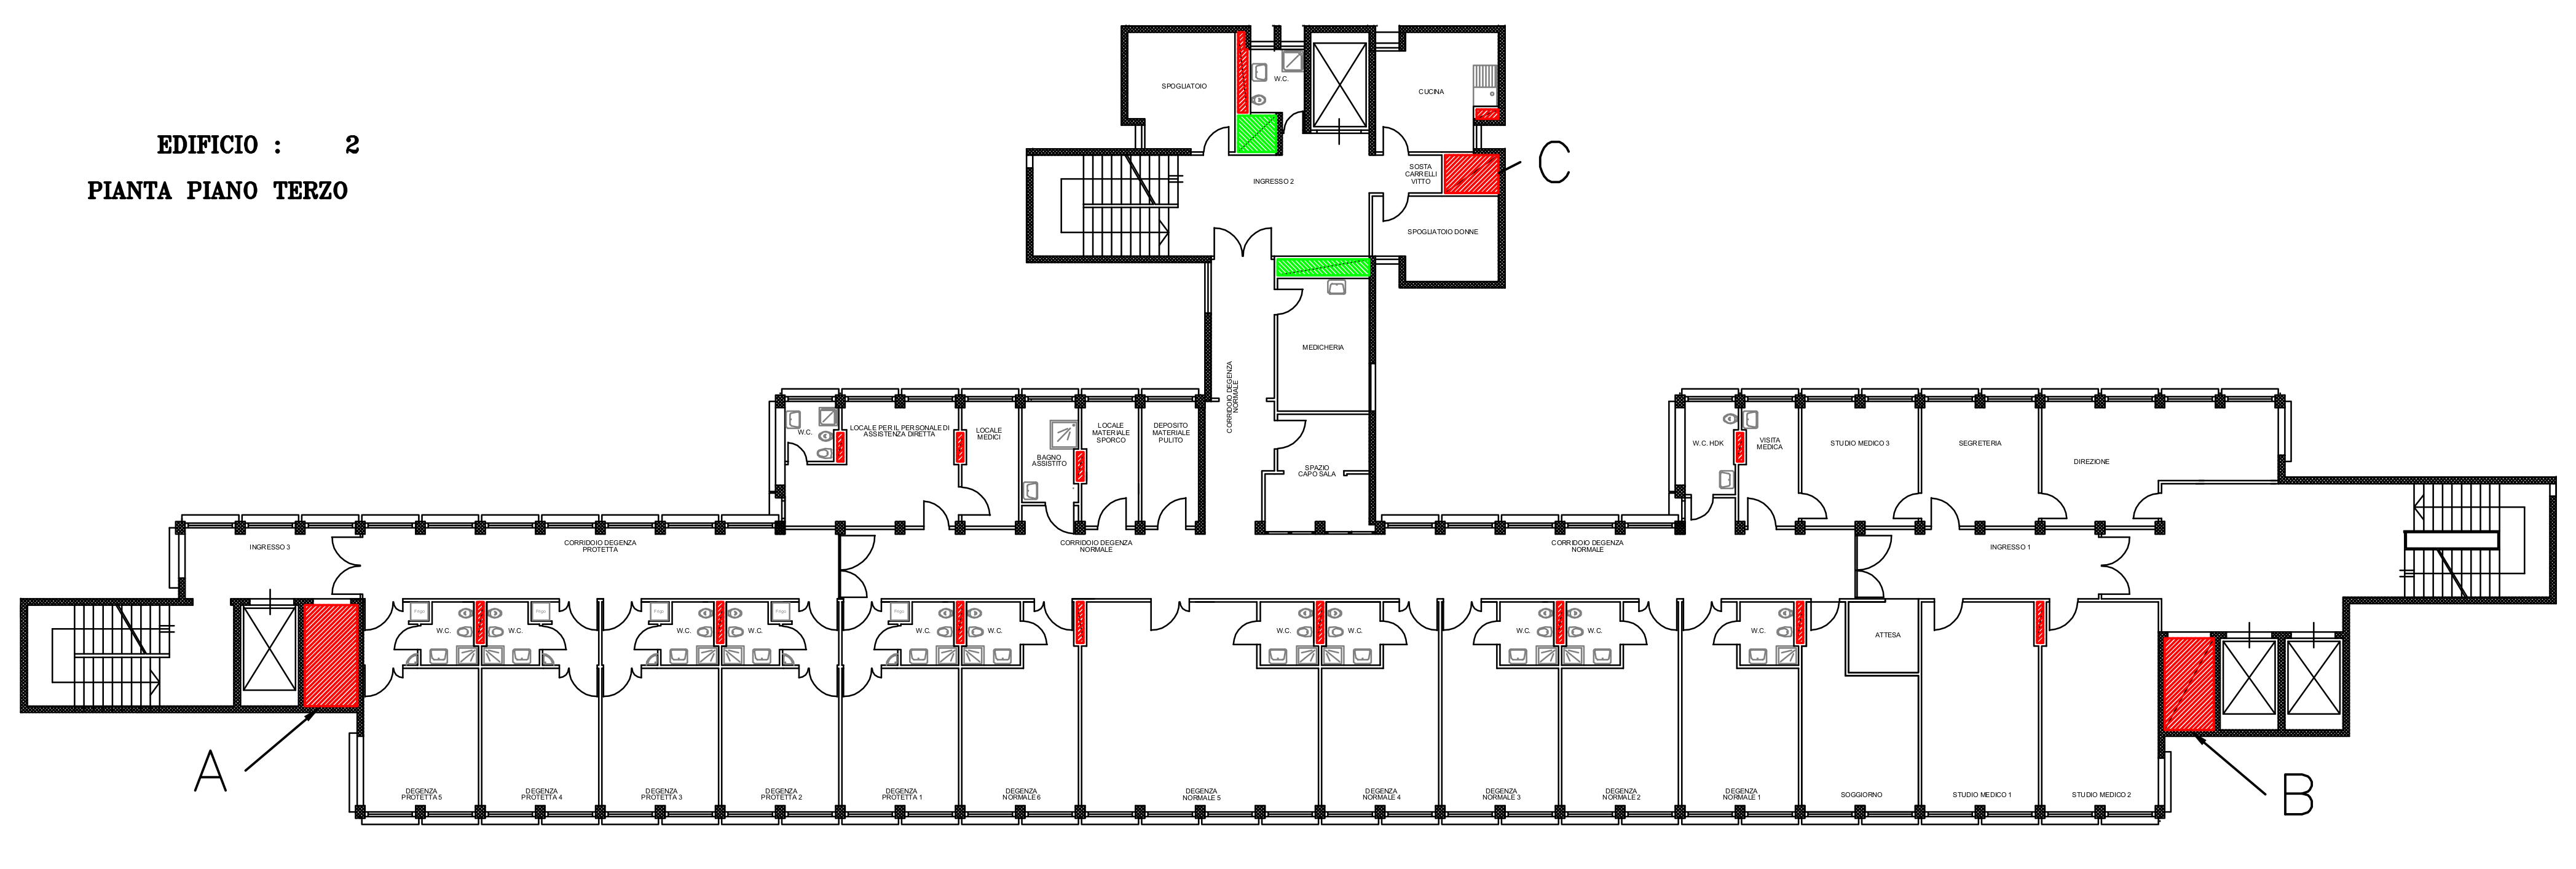
\includegraphics[width=\hsize]{6_4_cap/img/cavedi}
	\caption{Cavedi del Piano Terzo -- Corpo A}
	\label{img:cav}
\end{sidewaysfigure}
%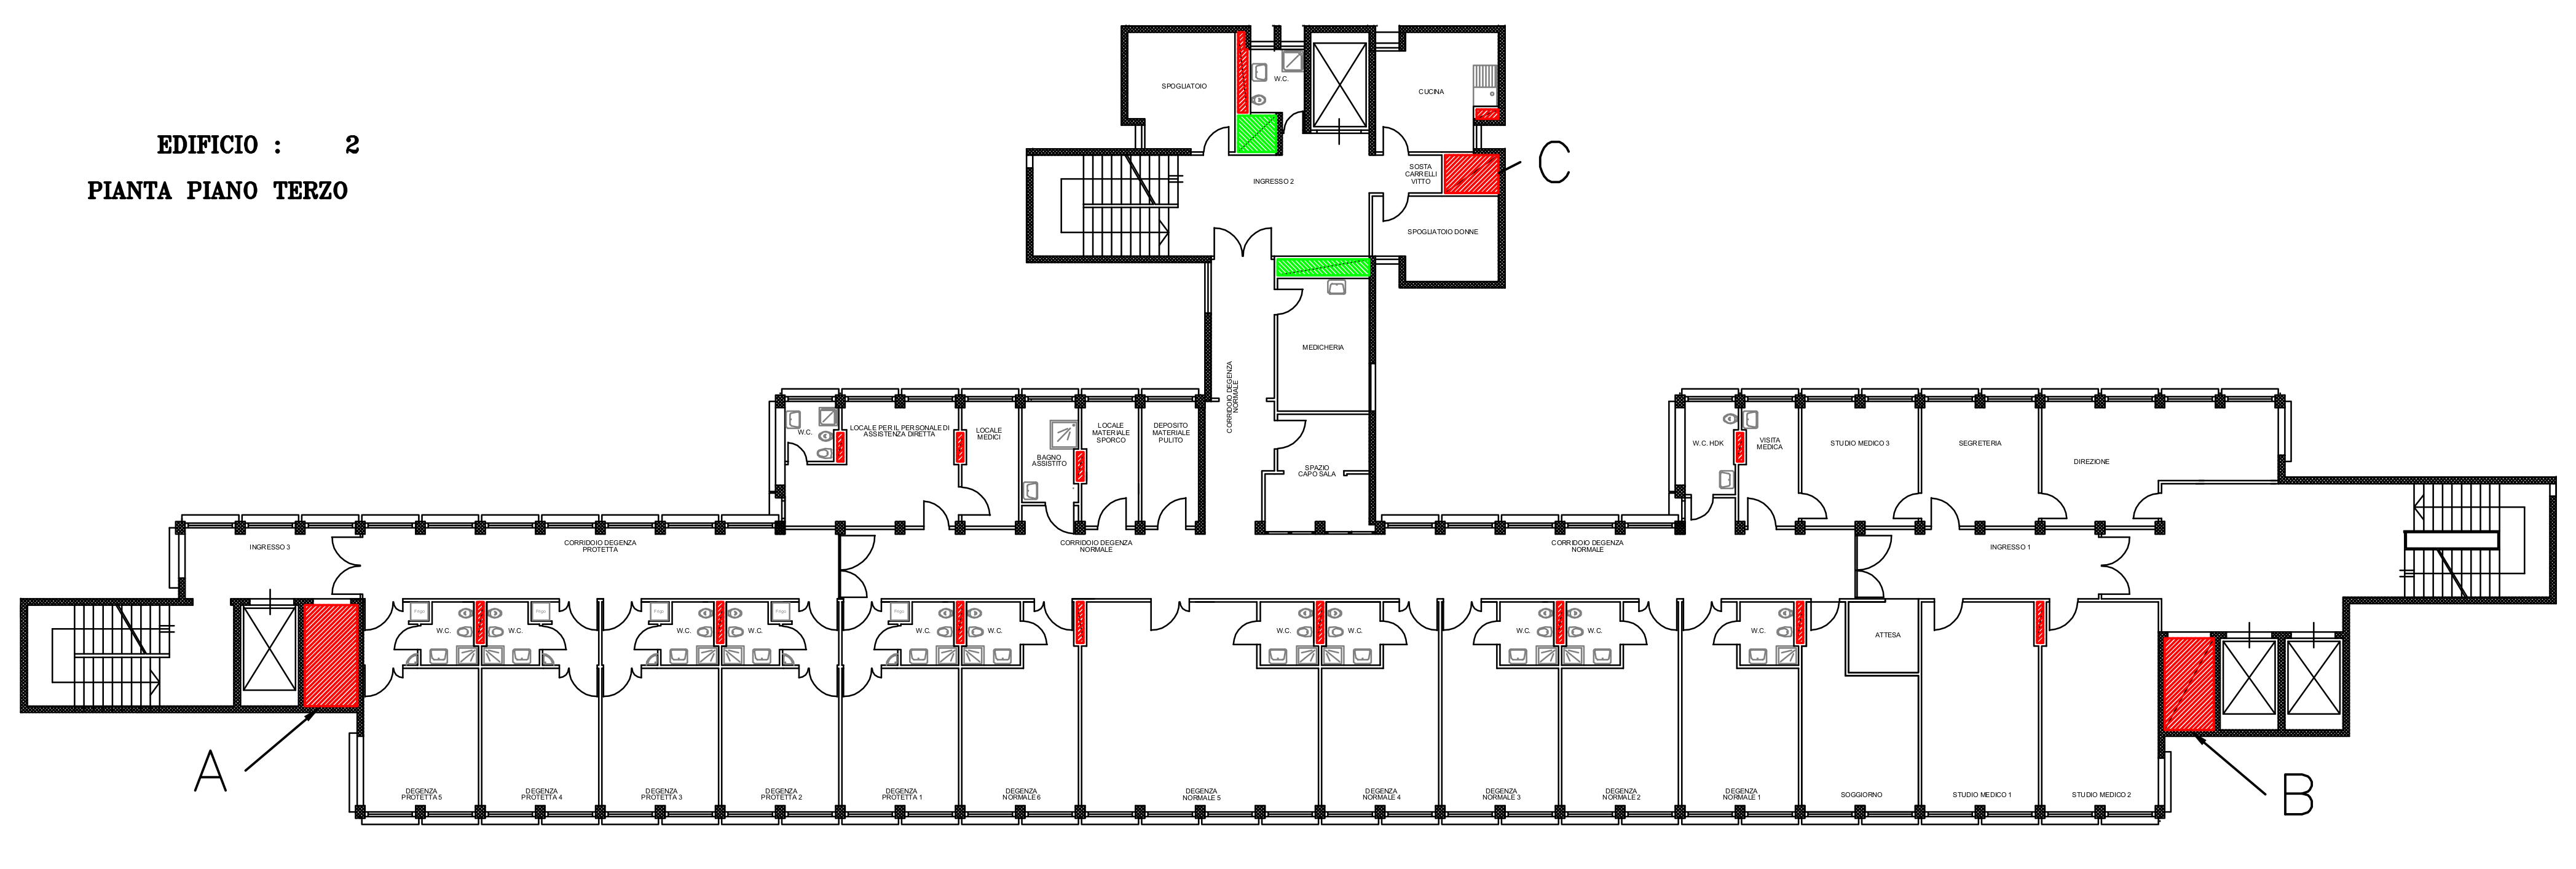
\includepdf{6_4_cap/img/cavedi}
I cavedi campiti in verde sono destinati alla rete elettrica. Tutti gli altri (in rosso) sono utilizzati dall'impianto idronico e aeraulico. In particolare, i 3 cavedi più grandi (i due adiacenti agli ascensori) e quello a destra nel torrino verranno utilizzati per le montanti dell'impianto a due tubi dei fancoil e dei radiatori. 

L'impianto dei fancoil è costituito da due tubi (una mandata e un ritorno). Vi saranno due montanti con una rete di distribuzione per ogni piano. Vista la configurazione essenzialmente longitudinale dell'edificio si è preferito costruire un circuito a \emph{ritorno inverso} con la montante di mandata che sale dal cavedio \textbf{A} e ritorna in quello \textbf{B}: in questo modo il \emph{ritorno inverso} è naturale. Per il torrino si è, invece, utilizzato il cavedio \textbf{C}. Lo \emph{switch} estate-inverno avviene in sottocentrale: in questo modo aumenta l'affidabilità di tutto l'impianto perché più semplice e con meno organi di regolazione.

L'impianto dei radiatori è pure a ritorno inverso e sfrutta i due cavedi \textbf{A} e \textbf{B}. 

I fancoil sono costituiti da una batteria alettata che scambia con l'aria in convezione forzata per la presenza di un ventilatore. Anche se vengono dimensionati per bilanciare il solo carico sensibile, quindi non si deve teoricamente formare la condensa, nella pratica lo fanno e pertanto possiedono sempre una vaschetta per l'eventuale acqua condensata. 

Scambiando per sola convezione, le temperature utilizzate nel caso estivo sono i famosi \num{7} - \n{12}{\degreeCelsius} e \num{50} - \n{45}{\degreeCelsius} nel funzionamento a caldo. 

I fancoil sono stati posizionati in tutti i locali eccetto i servizi igienici, spogliatoi e depositi vari.

Il dimensionamento è stato effettuato sfruttando la seguente relazione
\begin{equation}
	P=\dot{m}c\mathit{\Delta} T
\end{equation}
dove $P$ è la potenza termica sensibile, $\dot{m}$ è la portata d'acqua in \si{kg/s}, $c$ è il calore specifico dell'acqua e vale \n{4.2}{kJ/kgK} e il $\Delta T$ (differenza tra la temperatura di mandata e ritorno) vale \n{5}{\degreeCelsius}.

Per ogni locale (ovvero fancoil) si è calcolata la sua portata d'acqua necessaria per il funzionamento estivo e invernale. Il valore maggiore tra le due viene utilizzato per la scelta del diametro della tubazione. Alla fine si sommano tutte le portate per dimensionare la sotto-centrale. 

Per i radiatori si è proceduto nello stesso modo ricordando però \linebreak che $\Delta T=\SI{10}{\degreeCelsius}$.

Per entrambi gli impianti non si è provveduto ad inserire alcun organo di regolazione in quanto, essendo a \emph{ritorno inverso}, esso risulta bilanciato per natura. 

La tipologia dei fancoil è \emph{a soffitto} nel corpo A dove possibile (solitamente nelle degenze), \emph{a terra} nei corridoi e nel corpo C. In \vref{idr} è possibile vedere due figure della rete idronica dei due corpi. Si tratta di \emph{screenshot} dell'applicativo del software BIM della software-house C.A.T.S che permette, come è già stato detto precedentemente, di disegnare la rete, definire i carichi e calcolare la portata necessaria in ogni tratto dimensionandolo secondo criteri ben precisi. I rettangoli viola rappresentano i fancoil, quelli in rosso, invece, i radiatori. Come si nota, nelle degenze i fancoil non sono \emph{a soffitto} in quanto non esiste questa tipologia nel software. I risultati comunque non cambiano.

\begin{figure}
	\centering
	\subfloat[][\emph{Facciata meridionale}]{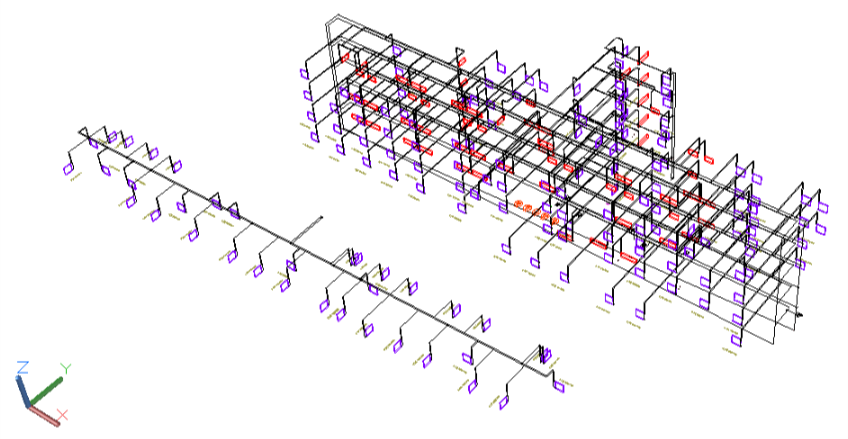
\includegraphics[width=\textwidth]{6_4_cap/img/idr1}\label{idr1}}\\
	\subfloat[][\emph{Facciata settentrionale}]{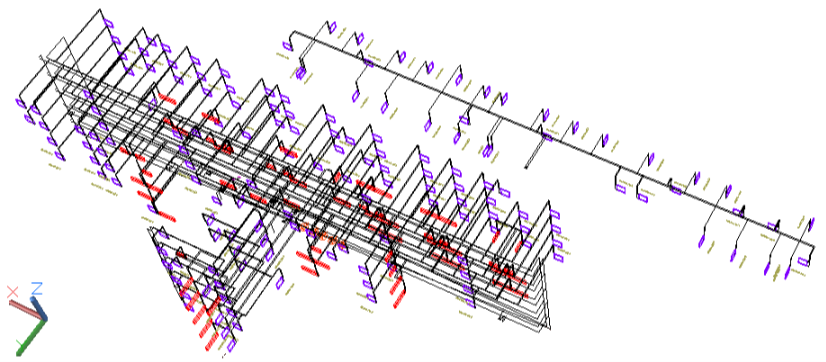
\includegraphics[width=\textwidth]{6_4_cap/img/idr2}\label{idr2}}
	\caption{Rete Idronica}\label{idr}
\end{figure}

\subsection{Impianto Aeraulico}
La portata di aria primaria per i corpi A e C è stata calcolata locale per locale utilizzando la \norvent. La rete aeraulica è stata disegnata su \textbf{CYPETHERM HVAC}. 

Non avendo spazio in cui posizionare le UTA, si sono usati dei recuperatori termodinamici. Tramite uno scambiatore a flussi incrociati, la portata di immissione e quella di estrazione vengono fatte entrare in contatto in modo tale che, in funzionamento estivo per esempio, la portata in uscita tenda a preraffreddare quella in ingresso. A valle di ciò, queste macchine possiedono anche un circuito a compressione di vapore le cui batterie alettate scambiano con la stessa portata di estrazione e immissione. Siccome le temperature dei due flussi sono vicine, queste pompe di calore hanno dei valori di efficienza (COP e EER) molto elevati.

Sono stati posizionati due recuperatori per piano nel corpo A (ma solo \num{1} al piano terra) nei pianerottoli delle scale antistanti i cavedi A e B. Nel corpo C vengono usati 4 recuperatori posizionati al piano \num{-1}.

Siccome queste reti aerauliche forniscono aria primaria ad un edificio ospedaliero, si vuole cercare di mantenere quanto è più pulito l'ambiente interno evitando infiltrazioni dall'esterno. Pertanto la portata di estrazione sarà minore di quella immessa in modo tale da generare un ambiente in sovrappressione rispetto l'esterno. Le velocità utilizzate per i canali di distribuzioni sono inferiori ai \n{3}{m/s} per contenere la rumorosità (oltre alle perdite di carico), mentre nei vari locali è stata diminuita a \n{2}{m/s}. Siccome l'impianto è \emph{misto}, la griglia di mandata dei fancoil viene sfruttata per immettere l'aria primaria della rete aeraulica in ambiente: in questo modo anche se la macchina idronica è spenta, l'impianto aeraulico può funzionare senza impedimenti o ostacoli. In \vref{aer} sono riportati due \emph{screenshot} di particolari della rete aeraulica dei due corpi mentre in \vref{img:aer} è presente la rete aeraulica intera del piano terzo come disegnata nell'applicativo \textbf{Load} di CYPE. 

\begin{figure}
	\centering
	\subfloat[][Vista meridionale]{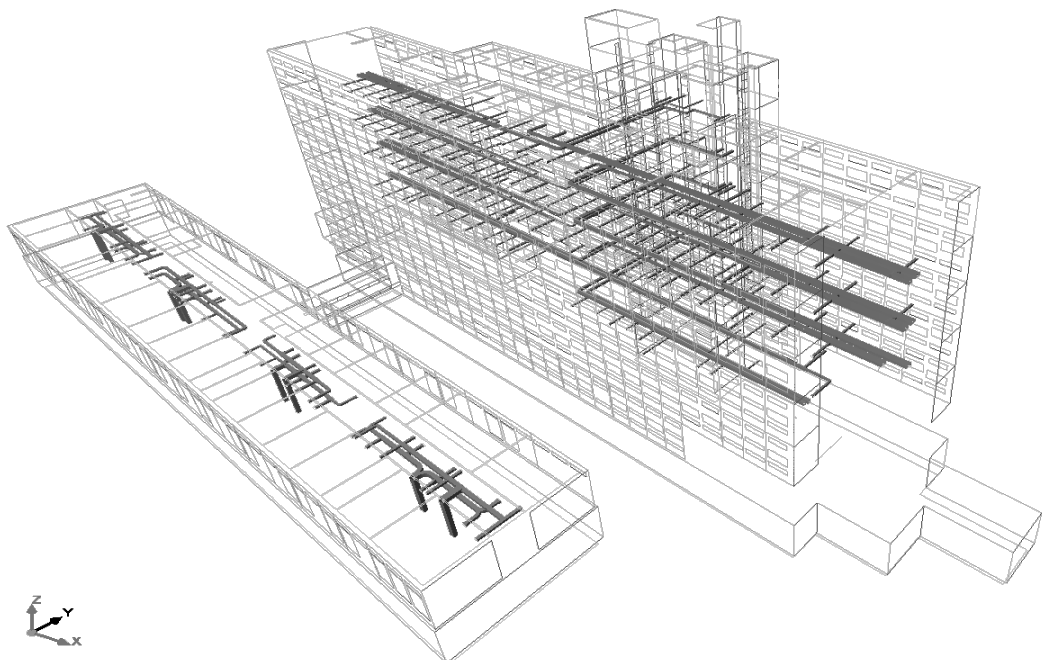
\includegraphics[width=0.9\textwidth]{6_4_cap/img/aer1}\label{aer1}}\\
	\subfloat[][Particolare del corpo C. Tramite il BIM è possibile disegnare e visualizzare in 3D.]{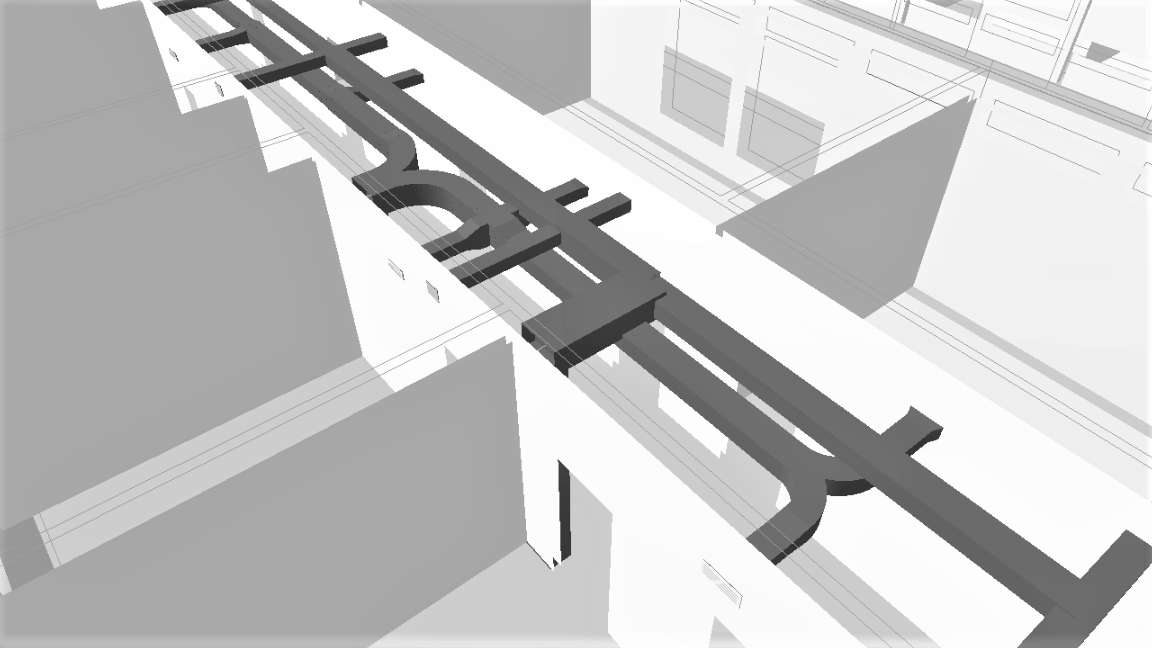
\includegraphics[width=0.9\textwidth]{6_4_cap/img/aer2}\label{aer2}}
	\caption[La rete aeraulica]{La rete aeraulica progettata con l'applicativo LOAD di CYPE}\label{aer}
\end{figure}
%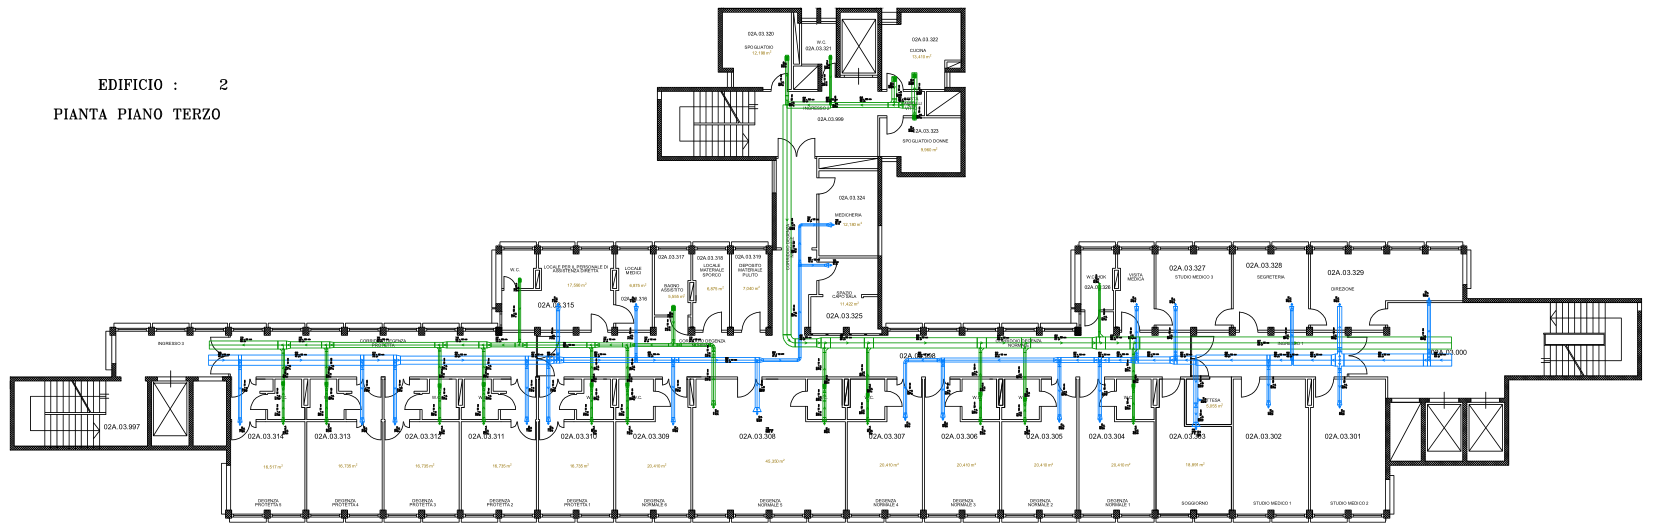
\includepdf{6_4_cap/img/aeraulica}
\begin{sidewaysfigure}
	\centering
	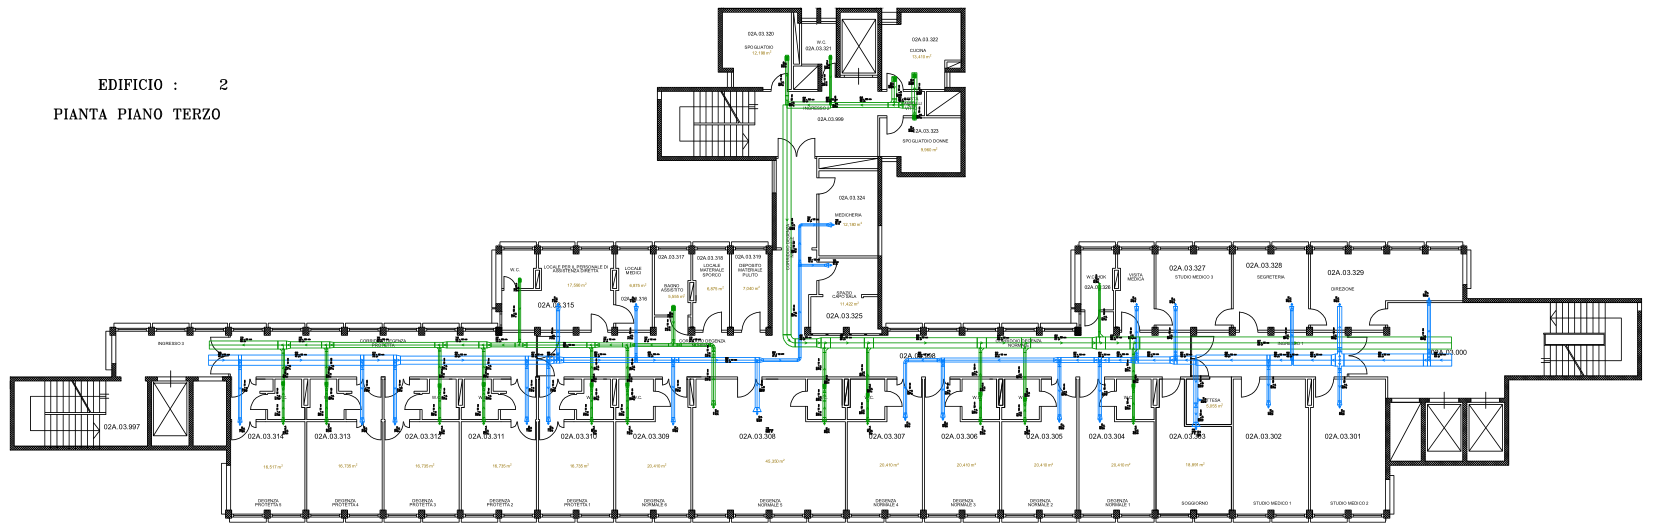
\includegraphics[width=\hsize]{6_4_cap/img/aeraulica}
	\caption{Rete Aeraulica Piano Terzo -- Corpo A}
	\label{img:aer}
\end{sidewaysfigure}
\section{L'impianto - Lato Sottocentrale}
Prima di procedere con la descrizione della sottocentrale che alimenta tutto il corpo di fabbrica dell'edificio 2, è doveroso elencare le utenze che usufruiranno dei servizi di acqua calda e refrigerata.
\begin{itemize}
	\item L'acqua calda è necessaria a diverse temperature per:
	\begin{itemize}
		\item Fancoil (\n{50}{\degreeCelsius});
		\item Radiatori (\n{80}{\degreeCelsius});
		\item Vecchi impianti, ovvero le UTA per il blocco operatorio, l'UTIC e l'emodinamica (\n{60}{\degreeCelsius});
		\item Acqua Calda Sanitaria (ACS).
	\end{itemize}
	\item L'acqua refrigerata è necessaria a \n{7}{\degreeCelsius} per:
	\begin{itemize}
		\item Fancoil;
		\item Vecchi impianti, ovvero le UTA per il blocco operatorio, l'UTIC e l'emodinamica.
	\end{itemize}
\end{itemize}
\subsection{Acqua Calda}
Come è già stato detto nel primo capitolo, in tutto il policlinico vi è una rete di presidio di acqua surriscaldata e refrigerata prodotta dai reflui termici del cogeneratore, caldaie e assorbitori. 

Per produrre acqua calda ad \n{80}{\degreeCelsius} si usa uno scambiatore dimensionato sulla $\dot{Q}_{\mathrm{risc,TOT}} = \sum \dot{Q}_{\mathrm{risc,i}}$ dove $\dot{Q}_{\mathrm{risc,i}}$ sono le potenze per il riscaldamento dei fancoil, UTA, radiatori delle varie zone termiche e dell'acqua calda sanitaria. La sommatoria non tiene conto delle potenze di ventilazione per i corpi A e C in quanto quel calore viene fornito (come anche nel caso estivo) dai recuperatori che possiedono un proprio impianto a compressione di vapore. Per questioni di sicurezza la $\dot{Q}_{\mathrm{risc,TOT}}$ viene aumentata di un \n{20}{\%} e vengono usati due scambiatori gemelli: in caso di guasto o manutenzione di una macchina, vi sarà l'altra ad assicurare la continuità del servizio.

In definitiva, essendo $\dot{Q}_{\mathrm{risc,TOT}}=\SI{600}{kW}$, sovradimensionando per sicurezza del \n{20}{\%} si ottengono \n{720}{kW}. 

Ogni scambiatore non verrà dimensionato sul massimo della potenzialità ma sui $2/3$ in quanto il picco si avrà solo in poche occasioni, per il resto del tempo (che rappresenta la maggior parte) ogni scambiatore lavorerà \emph{parzializzato}. Pertanto invece di dimensionare il singolo scambiatore sui \n{720}{kW}, si preferisce utilizzarne due da \n{480}{kW}. Nel funzionamento ordinario, sarà attivo un solo scambiatore mentre l'altro è di back-up. Nel caso ci siano esigenze particolari, si fa funzionare anche il secondo scambiatore. In caso di guasto o manutenzione (ordinaria e straordinaria) vi è l'altro scambiatore a garantire la continuità del servizio. Non bisogna dimenticare della presenza delle pompe di calore che comunque coprono una buona parte del carico. Quindi l'affidabilità e soprattutto la continuità del servizio sono garantite.

Il corretto funzionamento dello scambiatore (ovvero la produzione continua di acqua a \n{80}{\degreeCelsius}), viene assicurato da un termostato, posto nel ramo di mandata alle utenze, che, misurando continuamente la temperatura, invia un segnale ad una valvola a 3 vie a monte dello scambiatore (lato centrale) in modo tale da correggere la portata di acqua surriscaldata che fluisce nello scambiatore. 

In rispetto della \emph{Raccolta R} (elaborata dall'ISPESL -- Istituto Superiore per la Prevenzione e la Sicurezza del Lavoro -- e entrata in vigore nel \num{2011} con circolare INAIL -- Istituto Nazionale Assicurazioni e Infortuni sul Lavoro), a valle di entrambi gli scambiatori sono presenti tutti gli organi che assicurano \emph{Sicurezza}, \emph{Protezione} e \emph{Controllo} nei confronti di un impianto di generazione termica avente temperature di produzione massime non superiori a \n{110}{\degreeCelsius} e potenza nominale massima complessiva dei focolari superiore a \n{35}{kW}.

A monte e valle degli scambiatori sono presenti gli appositi strumenti per la contabilizzazione del calore:
\begin{itemize}
	\item flussometro: misura la portata di acqua che lo attraversa;
	\item 2 termostati: misurano la temperatura di mandata e ritorno e la comunicano ad un apposito controllore elettronico di temperatura (TC);
	\item TC: calcola la potenza utilizzata e la comunica al sistema informatico della sottocentrale. 
\end{itemize}
Solo con l'ausilio di questi strumenti è possibile conoscere effettivamente la potenza utilizzata e, di conseguenza, controllare se il comportamento dell'impianto è in linea con le ipotesi di progettazione.

La distribuzione dell'acqua a \n{80}{\degreeCelsius} viene affidata ad una coppia di pompe inverterate che portano il fluido all'unico collettore del secondario della sottocentrale dove ogni gruppo-pompe, uno per ogni servizio, alimenta la propria rete. 

La produzione di acqua a temperature inferiori per le batterie di pre e post riscaldamento delle UTA è affidata a valvole miscelatrici presenti sulla mandata: queste valvole miscelano la giusta portata di ritorno (ad una temperatura inferiore) e ad \n{80}{\degreeCelsius} in modo tale da ottenere la temperatura desiderata. Un termostato presente sulla mandata agisce direttamente sulla suddetta valvola a 3 vie.

Per il servizio fancoil (a \n{50}{\degreeCelsius}) si è optato per uno scambiatore, invece della valvola miscelatrice, per evitare che acqua a \n{80}{\degreeCelsius} entrasse durante la miscelazione nella rete stessa dei fancoil. In questo caso, però, bisogna ricordare che suddetta rete funziona con acqua calda in inverno e refrigerata in estate quando, però, bisogna garantire anche il servizio di acqua calda per le batterie di post-riscaldamento delle UTA.

Sul collettore del secondario a \n{80}{\degreeCelsius} vi è innestato anche il gruppo pompe per i bollitori dell'acqua calda sanitaria. Per il loro dimensionamento è stata utilizzata la UNI 9182. Si è proceduto in questo modo:
\begin{enumerate}
	\item Sono stati considerati 130 bagni in tutto il corpo A e C;
	\item la norma prevede per gli ospedali da \num{130} a \num{150} \si{l/persona} al giorno ($q_n$);
	\item la durata del periodo di punta dei consumi di acqua calda per gli ospedali vale 4 ore ($d$);
	\item si è determinato il massimo consumo orario contemporaneo di acqua calda a \n{40}{\degreeCelsius} usando la \vref{qm} dove $q_1=150$, $N=130$, $d=4$ e i tre fattori riduttivi per la contemporaneità sono unitari;
	\item Si è calcolato il volume del \emph{preparatore} (ovvero il bollitore) usando la \vref{preparatore};
	\item Si è calcolata la potenzialità termica da fornire al bollitore tramite l'acqua a \n{80}{\degreeCelsius} usando la \vref{serpentino}.
\end{enumerate}

\begin{equation}
q_M=\frac{q_1\times N_1}{d_1}\times f_1 \times f_2 \times f_3
\label{qm}
\end{equation}

\begin{equation}
	V_c=\frac{q_M \times d_p(T_m-T_f)}{d_p+P_r}\times \frac{P_r}{T_c-T_f}
	\label{preparatore}
\end{equation}

\begin{equation}
	W=\frac{q_M \times d_p (T_m-T_f)\times 1.163}{d_p+P_r}
	\label{serpentino}
\end{equation}

I risultati sono i seguenti:
\begin{itemize}
	\item $V_c = \SI{4400}{l}$ e quindi si useranno 2 bollitori da \n{5000}{l} per aumentare l'affidabilità del sistema;
	\item $W= \SI{120}{kW}$ e quindi la portata d'acqua a \n{80}{\degreeCelsius} sarà $\dot{m}_w\approx\SI{3}{kg/s}$ per bollitore.
\end{itemize}

\subsection{Acqua Refrigerata}
La produzione di acqua a \n{7}{\degreeCelsius} è affidata ad un mix di macchine ordinate in base alla priorità nel seguente elenco:
\begin{itemize}
	\item Assorbitori che sfruttano la rete di acqua surriscaldata di presidio;
	\item Pompe di calore con impianto geotermico.	
	\item Scambiatori che sfruttano la rete di acqua refrigerata di presidio;
\end{itemize}
Il cogeneratore ha \n{9}{MW} di reflui termici in estate di cui solo una parte vengono effettivamente utilizzati negli assorbitori i quali, al giorno d'oggi, non riescono a coprire il carico termico estivo di tutta la rete ospedaliera. Per questo motivo si è optata per l'installazione di un assorbitore in sottocentrale dedicato per il solo edificio 2: per sfruttare i reflui termici del cogeneratore che altrimenti verrebbero persi.

Le pompe di calore producono acqua refrigerata a \n{7}{\degreeCelsius} in estate e a \n{50}{\degreeCelsius} in inverno per i soli fancoil sul lato utenza, mentre scambiano con un apposito impianto geotermico.

Infine, gli scambiatori sfruttano la rete di presidio di acqua refrigerata per la fornitura del servizio in tutto l'edificio. In caso di guasto o manutenzione di una delle macchine di cui sopra, gli scambiatori permettono comunque di erogare al \n{100}{\%} il servizio.

Il mix così descritto permette di produrre acqua refrigerata con un'elevata affidabilità.
\subsubsection{L'assorbitore}
Di seguito è descritto il principio di funzionamento dei gruppi ad assorbimento, evidenziandone gli aspetti più significativi sotto il profilo impiantistico ed energetico. 

Le \emph{AHP} -- Absorption Heat Pump -- sebbene già sviluppate in età pioneristica (a partire dal 1860 circa), dopo un certo successo iniziale di mercato, con l'avvento dell'energia elettrica, furono soppiantate dalle \emph{EHP} -- Electric Heat Pump. Rispetto a queste ultime, le AHP presentano considerevoli vantaggi di tipo energetico ed ambientale, cui possono in alcuni casi accompagnarsi interessanti risparmi sui costi di esercizio.

Il principio di funzionamento si basa sulla capacità di particolari soluzioni chimiche (ottenute mescolando una sostanza \emph{refrigerante} ed una \emph{assorbente}) di assorbire continuativamente il vapore di refrigerante proveniente dall'evaporatore di una macchina frigorifera permettendo dunque che in quest'ultima l'evaporazione, e quindi l'effetto frigorigeno desiderato, siano continui.

Sono ancora presenti l'evaporatore ed il condensatore ma la compressione del vapore non è meccanica (scompare il compressore) ma termochimica (è presente un assorbitore/generatore). Al pari delle EHP, le AHP utilizzano l'evaporazione di un fluido \emph{refrigerante} per sottrarre energia termica dall'ambiente da climatizzare. Il refrigerante vaporizzato viene assorbito da una soluzione acquosa in cui è presente l'assorbente. Le coppie di fluidi di lavoro (refrigerante/assorbente) attualmente più utilizzate sono ammoniaca/acqua e acqua/bromuro di litio che è la più diffusa nelle macchine attualmente in commercio. Accanto alle funzioni di evaporazione ed assorbimento, per assicurare il funzionamento ciclico della macchina occorre far sì che l'assorbente, diluito nel refrigerante, riacquisti la sua capacità assorbente iniziale. A questo scopo viene introdotta una fase di rigenerazione: dall'assorbitore la miscela ricca di refrigerante viene inviata in un ulteriore dispositivo, il generatore, dove, per effetto di un'adduzione d'energia termica, si impoverisce di refrigerante; in tal modo, si ripristinano le condizioni iniziali delle fasi di evaporazione ed assorbimento.

Nelle applicazioni attuali si distinguono due tipologie di macchine ad assorbimento: quelle ad \emph{alimentazione indiretta} e quelle a \emph{fiamma diretta}.

Alla prima categoria appartengono quelle macchine che utilizzano come fluido caldo di alimentazione acqua surriscaldata (\num{115} + \n{132}{\degreeCelsius}, o anche temperature molto inferiori) o vapor d'acqua (\num{60} + \n{80}{kPa}) che fluisce all'interno di uno scambiatore posto nel generatore. La produzione del fluido caldo può essere affidata ad un generatore di vapore, oppure è possibile utilizzare i reflui termici di motori endotermici o dei processi industriali.

Nei gruppi a fiamma diretta, nel generatore avviene il riscaldamento direttamente con un bruciatore, solitamente alimentato a gas naturale.

Le prestazioni delle AHP decrescono al crescere della temperatura media cui è ceduta la potenza termica dell'assorbitore e del condensatore. Ciò ha in generale imposto l'adozione della condensazione ad acqua anziché ad aria. Ovviamente la temperatura dell'acqua resa disponibile dalla torre condiziona fortemente la resa frigorifera delle AHP: quest'ultima si riduce del \n{20}{\%} per un incremento di temperatura dell'acqua di raffreddamento di soli \n{2}{\degreeCelsius}.

A causa dei più bassi COP realizzabili dalle AHP rispetto alle macchine a compressione di vapore condensate ad acqua (tipicamente \num{0.6} + \num{0.7} le prime, \num{3} + \num{5} le seconde), il fabbisogno d'acqua di raffreddamento è in generale notevolmente superiore (\num{1.5} + \num{2.1} volte) rispetto a quello di una corrispondente macchina a compressione di vapore. 

L'adozione delle torri di raffreddamento evaporativo da un lato permette di avere l'acqua di raffreddamento del condensatore e dell'assorbitore in un livello di temperatura abbastanza basso, \num{28} + \n{34}{\degreeCelsius}, da un altro rappresentano un ulteriore complicazione del sistema. Si ha, inoltre, l'introduzione di una fonte di rumore in una macchina che è di per sè molto silenziosa. Comunque, per macchine di taglia elevata, i costi di abbattimento del rumore per le AHP rimangono inferiori rispetto a quelli delle macchine a compressione di vapore. 

Nelle macchine a \emph{semplice effetto} o \emph{monostadio}, il COP, a causa delle irreversibilità presenti, è sempre inferiore a \num{1} con valori intorno a \num{0.7} per le macchine ad alimentazione indiretta (tipicamente ad acqua a \num{80} + \n{90}{\degreeCelsius} per le macchine a acqua e bromuro di litio e a vapore a \num{130} + \n{140}{\degreeCelsius} per quelle ad ammoniaca) ed intorno a \num{0.6} per quelle a fiamma diretta. La limitazione sul valore del COP è superata con macchine più complesse a \emph{doppio effetto} o \emph{bistadio}. In estrema sintesi, rispetto allo schema della macchina monostadio è inserito un secondo generatore a più alta temperatura e pressione (\emph{generatore ad alta temperatura}) che interagisce con l'esterno in modo diretto (fiamma diretta) od indiretto (alimentazione a vapore oltre \n{180}{\degreeCelsius}).

Il vapor d'acqua prodotto internamente a questo generatore ha una temperatura sufficientemente elevata per essere impiegato nel secondo stadio (\emph{secondo generatore}); in esso, a temperatura e pressione prossime a quella del monostadio, condensando realizza, senza ulteriore spesa, un'ulteriore concentrazione/generazione. Da questo punto in poi il circuito è equivalente a quello del monostadio con la differenza che nell'AHP a doppio stadio un'unità di massa prodotta nel generatore ad alta temperatura può fare evaporare , rispetto al monostadio, un'ulteriore unità di massa di refrigerante nel generatore a bassa temperatura, e quindi avere nell'evaporatore l'evaporazione di due unità di massa di refrigerante. il COP massimo raggiunto da queste apparecchiature si aggira intorno a \num{1.3} per le macchine ad alimentazione indiretta e intorno all'unità per quelle a fiamma diretta.

In definitiva, si può affermare che, rispetto alle tradizionali apparecchiature a compressione di vapore, gli assorbitori offrono i seguenti vantaggi:
\begin{itemize}
	\item rispetto delle normative ecologiche per il mancato impiego di fluidi clorofluoroderivati;
	\item l'utilizzo dell'energia elettrica è per il solo azionamento degli organi ausiliari: ciò comporta una drastica riduzione, rispetto ai tradizionali gruppi elettrici:
	\begin{itemize}
		\item del fabbisogno di energia elettrica (nel rapporto \num{1} a \num{10});
		\item della potenza elettrica assorbita.
	\end{itemize}
	\item sostanziale assenza di parti in movimento, con drastica riduzione di vibrazioni e rumorosità, mentre i gruppi a compressione impongono spesso costose opere di insonorizzazione;
	\item buona durata ed affidabilità;
	\item ottime prestazioni ai carichi parziali.
\end{itemize}
Di contro ci sono alcuni svantaggi:
\begin{itemize}
	\item modesto COP;
	\item necessità di ricorrere ad acqua di torre per la condensazione, soprattutto per gli assorbitori ad acqua/bromuro di litio;
	\item per gli assorbitori ad acqua/bromuro di litio, la necessità di ricorrere ad un'accurata gestione e manutenzione per quanto riguarda la tenuta al vuoto, indispensabile per il loro corretto funzionamento e per evitare l'insorgenza di corrosione;
	\item accurato controllo della temperatura dell'acqua di raffreddamento del condensatore/evaporatore in quanto, nel caso in cui sia troppo bassa, rischia di solidificare il bromuro di litio (in relazione alla sua concentrazione). Infatti, sul ritorno dell'acqua di torre vi è termostato che misura la temperatura: nel caso in cui questa sia troppo bassa, agisce su una valvola miscelatrice posta sul ritorno dell'acqua di torre bypassando di fatto la torre di condensazione stessa e facendo tornare all'assorbitore/condensatore acqua calda.
\end{itemize}
Tornando nell'ambito progettuale di questo elaborato di laurea, avendo in estate i reflui termici del cogeneratore utilizzabili mediante l'acqua surriscaldata a \n{130}{\degreeCelsius}, si è preferito utilizzare un assorbitore.

Le caratteristiche della macchina, per quello che è stato detto nella teoria, saranno le seguenti: \emph{alimentazione indiretta}, \emph{bistadio} e come fluido \emph{acqua e bromuro di litio}. Si è fissato il COP ad un cautelativo \num{1.25}. 

L'assorbitore è stato dimensionato sul carico massimo estivo. Si spera che in questo modo sia possibile utilizzare quanti più reflui termici essendo questi gratuiti (in quanto il \emph{goal} del cogeneratore è la produzione di energia elettrica per il policlinico).

La potenza termica di raffreddamento è $\dot{Q}_{\mathrm{raff}}=\SI{730}{kW}$ e sovradimensionando di un coefficiente di sicurezza pari al \n{20}{\%} si ottiene $\dot{Q}_{\mathrm{raff}}=\SI{900}{kW}$ che sarà la potenzialità dell'assorbitore.

Scrivendo la relazione del COP,
\begin{equation}
	COP=\frac{\dot{Q}_{EV}}{\dot{Q}_{GE}}
\end{equation}
è possibile quantificare la potenza necessaria al generatore e quindi valutare la portata di acqua surriscaldata necessaria. 
\begin{align}
	\dot{Q}_{GE} &= \SI{720}{kW}\\
	\dot{m}_w &= \frac{\dot{Q}_{GE}}{c\ \mathit{\Delta} T}\label{Portata}\\
	\dot{m}_w&=\SI{5.7}{kg/s}\label{Portata:acquacalda}
\end{align}
nella \vref{Portata} si è fissato $\mathit{\Delta} T=\SI{30}{\degreeCelsius}$.

Siccome per gli assorbitori vale il seguente bilancio energetico
\begin{equation}
	\dot{Q}_{GE}+\dot{Q}_{EV}=\dot{Q}_{CO}+\dot{Q}_{ASS}
\end{equation}
sarà che la potenza da sottrarre al condensatore e all'assorbitore (e quindi da smaltire in atmosfera mediante la torre evaporativa) vale
\begin{equation}
	\dot{Q}_{CO}+\dot{Q}_{ASS}=\SI{1620}{kW}
\end{equation}
e quindi, per il solito coefficiente di sicurezza, si dimensionerà la torre evaporativa su una potenzialità pari a $\dot{Q}_{TORRE}=\SI{1900}{kW}$, il che necessita di una portata d'acqua pari a (con $\Delta T=\SI{5}{\degreeCelsius}$)
\begin{equation}
	\dot{m}_w\approx \SI{90}{kg/s}
\end{equation}

\subsubsection{La pompa di calore e l'impianto geotermico}
Il principio di funzionamento di tali sistemi si basa sul cambiamento di fase del liquido frigorigeno lungo il ciclo termodinamico che quest'ultimo compie. Il raffreddamento è in generale ottenuto dall'evaporazione del refrigerante ad una temperatura e ad una pressione che sono le più basse al'interno del ciclo. Queste ultime sono successivamente innalzate attraverso la compressione meccanica del fluido frigorigeno che alla fine di tale processo è vapore surriscaldato ad una temperatura e ad una pressione che sono le più alte all'interno del ciclo. Il riscaldamento, cioè la somministrazione d'energia termica dal sistema all'ambiente, è ottenuto attraverso il desurriscaldamento del fluido frigorigeno e la sua successiva condensazione. Il ciclo si completa attraverso l'espansione del suddetto fluido attraverso un apposito organo fino alle condizioni in cui ricomincia il processo d'evaporazione. Sono per quanto detto presenti quattro trasformazioni compiute attraverso quattro distinti componenti.

Dal medesimo ciclo termodinamico possono dunque ottenersi sia un impianto \emph{frigorifero} che un impianto a \emph{pompa di calore}. In entrambi i casi è possibile definire un COP (\emph{Coefficient Of Performance}). 

Per quanto riguarda il fluido refrigerante evolvente nell'impianto, è necessario che quest'ultimo abbia delle particolari caratteristiche termodinamiche, economiche e d'impatto ambientale, tra cui:
\begin{itemize}
	\item la possibilità che il ciclo termodinamico possa essere collocato nella regione dei vapori saturi. Ciò deve verificarsi anche a temperature molto basse senza che compaia la fase solida;
	\item una curva della tensione di vapore tale che non si generino eccessiva pressioni e depressioni rispettivamente al condensatore ed all'evaporatore;
	\item una variazione di entalpia d'evaporazione sufficientemente alta tale che, a parità di potenza termica scambiata, siano necessarie portate di refrigerante e quindi costi di compressioni contenuti;
	\item un volume specifico non troppo grande in modo tale che il lavoro di compressione, le dimensioni dei condotti e del compressore non eccedano;
	\item un costo d'acquisto ridotto, una bassa tossicità e una buona stabilità chimica rispetto ai materiali che costituiscono l'impianto;
	\item un basso impatto ambientale nei riguardi del \emph{buco dell'ozono} e dell'\emph{effetto serra}.
\end{itemize}
Riguardo a quest'ultimo punto, i fluidi frigorigeni moderni di più largo impiego sono dal punto di vista chimico degli HFC (\emph{Hydro Fluoro Carburi}: R407C, R410a, R134a, ecc\dots) composti in cui, per limitare il problema legato alla comparsa dell'ozono sui poli terrestri, è assente rispetto ai vecchi refrigeranti (CFC, HCFC) la molecola del cloro (ritenuta appunto fra i responsabili del \emph{buco dell'ozono}). Ultimamente l'attenzione è posta anche nello scegliere fluidi refrigeranti che limitino l'assorbimento della radiazione infrarossa e cioè l'effetto serra. L'R134a è, ad esempio, uno di quelli che maggiormente causa tale fenomeno.

Vengono di seguito illustrate le caratteristiche di funzionamento delle pompe di calore a compressione di vapore in base alla sorgente o pozzo d'energia termica utilizzata.

\paragraph{L'aria}
È quella utilizzata più frequentemente. Lo scambiatore di calore esterno all'ambiente da climatizzare è in questo caso caratterizzato da un'estesa superficie di scambio termico. Ciò è dovuto alla modesta efficienza della trasmissione del calore causata dal basso coefficiente di scambio termico di un aeriforme qual è l'aria in convezione forzata. Per questa ragione lo scambiatore esterno è generalmente costituito da una batteria alettata. 

L'efficienza della pompa di calore dipende moltissimo dalla temperatura ambiente. Nel caso invernale, per esempio, quanto più è bassa la temperatura esterna, tanto più diminuisce il COP quando invece il carico di riscaldamento dell'edificio aumenta.

Nel caso le temperature esterne invernali scendono continuativamente sotto o sono prossime allo zero, vi è il problema della formazione di \emph{brina} sulla batteria alettata esterna che provoca la diminuzione di superficie di scambio termico effettivamente utile. Ciò provoca un abbassamento dell'efficienza dell'evaporatore (sempre in caso invernale) e la fuoriuscita dallo stesso di una miscela di vapore e liquido di refrigerante. La risposta della centralina di controllo è un nuovo abbassamento della pressione di saturazione all'evaporatore (e quindi della sua temperatura di saturazione) che provoca una formazione di brina ancora più spinto. È necessario, quindi, effettuare lo \emph{sbrinamento}: riscaldare in qualche modo la batteria dell'evaporatore. Questo comporta \emph{discomfort} per l'utenza interna o, nel migliore dei casi, una semplice interruzione del servizio di riscaldamento.

Quindi, siccome il funzionamento di una pompa di calore dipende moltissimo dalle caratteristiche termodinamiche ambientali, si cercano altre forme di SET in cui la variazione di temperatura sia quanto più contenuta possibile. Al sud Italia l'impiego delle pompe di calore durante tutta la stagione invernale è molto più favorevole che al centro o al nord dove tipicamente nei mesi di gennaio e febbraio si rischia la formazione di brina.

\paragraph{L'acqua}
L'acqua può essere una sorgente (o pozzo) d'energia termica ottimale. Nel caso venga adottata la configurazione con torre evaporativa è affidata a quest'ultima il compito di raffreddare l'acqua proveniente dal condensatore. La torre, attraverso la saturazione dell'aria di processo raffredda per effetto dell'evaporazione l'acqua proveniente dal condensatore. La saturazione è ottenuta grazie alla fine nebulizzazione dell'acqua di processo che può appartenere ad un circuito separato da quello del condensatore, oppure provenire direttamente da quest'ultimo. Ovviamente il potenziale di raffreddamento è limitato e rappresentato, nel caso ideale di efficienza unitaria della torre evaporativa, dalla temperatura di bulbo bagnato dell'aria di processo proveniente dall'esterno. Nella realtà l'efficienza delle torri evaporative è ben lontana dal \n{100}{\%}. Notevole attenzione va prestata alla manutenzione del sistema necessaria anche per scongiurare il pericolo dell'insorgenza di funghi e infezioni come la \emph{legionella} dovuti alla presenza del necessario ristagno d'acqua. L'aria è movimentata da un ventilatore che insieme al consumo d'acqua e alla suddetta manutenzione rappresentano i costi di esercizio della torre.

Nel caso in cui sia possibile utilizzare la configurazione con \emph{circuito aperto} i vantaggi sono molteplici. Innanzitutto l'inerzia termica della sorgente (mare, fiumi, laghi, falda, ecc\dots) garantisce in generale una temperatura stabile per gran parte dell'anno, le fluttuazione sono infatti estremamente lente, dell'ordine di qualche giorno per grado di variazione. Un ulteriore vantaggio è rappresentato, a seconda della stagione, dall'elevata o bassa temperatura della sorgente. In estate ad esempio nel caso dell'acqua di mare, basta scendere di circa \n{10}{m} sotto la superficie per trovare una temperatura compresa tra gli \num{8} e i \n{12}{\degreeCelsius}.

\paragraph{L'energia solare}
In inverno uno dei principali vantaggi nell'utilizzo della radiazione solare come sorgente d'energia termica nelle pompe di calore è l'elevato valore della temperatura rispetto alle altre sorgenti con conseguente aumento del COP. Rispetto all'utilizzo dell'energia solare senza pompa di calore, l'efficienza e la potenza termica unitaria dei collettori solari è incrementata dalla minor temperatura richiesta al collettore. Vista l'enorme variabilità della radiazione solare durante la giornata, è molto importante accoppiare un impianto di collettori solare ad un accumulo termico correttamente dimensionato.

\paragraph{Il terreno}
La temperatura del terreno ad una certa profondità si stabilizza ad un valore molto prossimo a quello della media annuale della temperatura dell'aria. Ad elevate profondità, invece, entra in gioco l'energia termica endogena. Infatti, oltre i \n{30}{m} di profondità si riscontra in media un incremento di temperatura di circa \n{1}{\degreeCelsius} ogni \n{30}{m}. La temperatura del terreno è quindi più stabile di quella dell'aria esterna, non risente delle oscillazioni giornaliere, le variazioni di temperatura sono smorzate e ritardate di fase. Il tutto è tanto più vero quanto maggiore è la profondità. Le pompe di calore che utilizzano il terreno come sorgente di calore in inverno e pozzo di calore in estate sono dunque vantaggiose.

Questo tipo di pompe di calore prevede l'interramento di tubi di adeguata lunghezza attraverso due differenti tecniche: tubi orizzontali o tubi verticali. I sistemi a tubi orizzontali vengono interrati a piccola profondità (\num{0.8} + \n{1.5}{m}) trovando posto di solito sotto un'ampia superficie sgombra da edifici. I tubi devono resistere alla corrosione per periodi molto lunghi. Per questo motivo in passato si sono utilizzati spesso tubi in rame, mentre più recentemente si preferisce ricorrere a materie plastiche come il \emph{polietilene ad alta densità} ed il \emph{polibutilene rinforzato}. Le materie plastiche mentre risolvono il problema della corrosione e diminuiscono i costi, sono ovviamente caratterizzate da minori conduttività termiche rispetto ai metalli.

I sistemi a tubi verticali, invece, utilizzano una o più perforazioni con profondità variabili da valori minimi di \n{10}{m} a valori massimi che possono superare i \n{200}{m}. A tali profondità le temperature del terreno non risentono quasi più degli effetti superficiali. Inoltre la superficie in pianta richiesta è molto ridotta rispetto al caso precedente. Si possono utilizzare le stesse profondità dei pali di fondazione dell'edificio oppore raggiungerne maggiori. 

Le macchine che adottano tale tecnologia possono utilizzare un fluido secondario all'interno del circuito di tubi immerso nel terreno, che può essere acqua nei climi più miti o una miscela acqua-fluido anticongelante in quelli più rigidi. I fluidi anticongelanti più utilizzati sono il metanolo, l'etanolo e il glicol propilenico. In alternativa le macchine possono essere ad espansione diretta se utilizzano viceversa direttamente il fluido refrigerante nel circuito immerso nel terreno.

\vspace{1em}
Nella progettazione della sottocentrale si è stati obbligati ad utilizzare come sorgente/pozzo di energia termica il terreno.

Innanzitutto è stato necessario capire come modellare il terreno. In assenza di dati, sono stati utilizzati quelli dell'adiacente ``Istituto Nazionale Tumori - IRCCS \emph{Fondazione G. Pascale}'' in cui è stato costruito un campo geotermico e per l'occasione sono stati effettuati dei carotaggi per la valutazione del sottosuolo.

I dati ricavati relativi al terreno sono:
\begin{itemize}
	\item conducibilità termica: $\lambda = \SI{0.79}{W/mK}$;
	\item temperatura indisturbata: $T_g=\SI{15.4}{\degreeCelsius}$
	\item capacità termica: $c=\SI{1.5}{MJ/m^3K}$
\end{itemize}

La difficoltà nella progettazione del campo geotermico risiede nella complessa valutazione di scambi energetici che il terreno ha con il resto dell'ambiente. Infatti, la temperatura del terreno dipende da 3 tipologie di fenomeni:
\begin{itemize}
	\item scambio d'energia con l'atmosfera: irraggiamento solare, eventi meteorici, trasmissione per convezione (a cui si aggiunge la variabilità del vento), calore estratto dalla vegetazione e calore scambiato con gli edifici soprastanti;
	\item scambio d'energia con gli acquiferi che, a seconda della stagione, possono apportare od estrarre energia;
	\item apporto energetico legato al flusso geotermico.
\end{itemize}
Purtroppo anche considerando e studiando questi fenomeni singolarmente, il bilancio globale non è determinabile banalmente tramite sovrapposizione degli effetti in quanto è necessario tenere conto della mutua influenza. Sono necessari modelli matematici complessi, da sviluppare caso per caso.

La procedura di calcolo utilizzata per il dimensionamento delle sonde geotermiche verticali è quello proposto dalla ASHRAE: tale metodo, infatti, si rifà a quello analitico basato sulla teoria della sorgente cilindrica sviluppato da \emph{Ingersoll} e \emph{Zobel} nel 1954 e ripreso da \emph{Kavanaugh} e \emph{Rafferty} nel 1997.

Il modello analitico ha dato risultati utili per una buona progettazione del campo geotermico i quali vengono riassunti di seguito.
\begin{itemize}
	\item in fase di esercizio dell'impianto geotermico, il funzionamento della pompa di calore, sopratutto in condizioni di massimo carico, può provocare un decremento eccessivo della temperatura del terreno intorno alla sonda e dunque anche del fluido termovettore: tale situazione genera pericoli di gelo e stress meccanici tra terreno e sonda, che potrebbero minare l'incolumità della sonda stessa;
	\item per operare un corretto dimensionamento della sonda, è necessario conoscere i carichi termici dell'edificio e il loro andamento temporale, in particolare il carico medio annuale standard, il carico mensile massimo e quello orario di punta, sia nel caso invernale che estivo;
	\item gli impianti geotermici costituiti da molteplici sonde devono garantire distante reciproche sufficienti tra le stesse, in modo da garantire che i campi termici rispettivi non si influenzino reciprocamente. 
\end{itemize}
La relazione utilizzata dall'ASHRAE tiene conto della variazione temporale dei flussi termici scambiati tra sonda e terreno e quindi del differente significato che assume la resistenza del terreno al variare del periodo dell'oscillazione del flusso termico. Dal punto di visto matematico, si tiene conto di questo fenomeno facendo riferimento a tre ``impulsi termici'' a gradino di durata differente, mediante una semplice sovrapposizione degli effetti di breve, di medio e di lungo termine. Per ciascun gradino si introduce la resistenza termica del terreno corrispondente all'intervallo di tempo considerato; gli effetti dei tre impulsi vengono sommati, tenendo conto dei carichi termici corrispettivi.

Le relazioni, una per il caso invernale e l'altra per quello estivo, sono:
\begin{align}
	L_c&= \frac{\Phi_a R_{ga}+(\Phi_{lc}-W_{c})(R_b+PLF_mR_{gm}+R_{gd}F_{sc})}{T_0-\frac{T_{fi}+T_{fo}}{2}-T_p}\\
	L_h&= \frac{\Phi_a R_{ga}+(\Phi_{lh}-W_{h})(R_b+PLF_mR_{gm}+R_{gd}F_{sc})}{T_0-\frac{T_{fi}+T_{fo}}{2}-T_p}
\end{align}
dove:
\begin{description}
	\item[$\mathbf{L_c} \-- \mathbf{L_h}$] sono le lunghezze di perforazione necessarie per soddisfare rispettivamente il carico estivo (\emph{cooling}) od invernale (\emph{heating}) (il valore maggiore tra i due definisce la profondità di installazione da adottare), in \si{m};
	\item[$\mathbf{\Phi_a}$] è il flusso termico medio scambiato con il sottosuolo in un anno, in \si{W};
	\item[$\mathbf{\Phi_{lc}} \-- \mathbf{\Phi_{lh}}$] sono i carichi termici di progetto rispettivamente in raffrescamento ($\Phi_{lc}<0$) e in riscaldamento ($\Phi_{lh}>0$) dell'edificio, in \si{W};
	\item[$\mathbf{W_c} \-- \mathbf{W_h}$] sono le potenze elettriche assorbite dal compressore della pompa di calore al carico termico estivo ed invernale di picco, in \si{W};
	\item[$\mathbf{R_{ga}}$] è la resistenza termica lineare equivalente del terreno per un impulso annuale, in \si{mK/W}. Serve a tenere conto dell'andamento della temperatura del terreno sul lungo periodo, sostanzialmente identificabile con la durata dell'impianto. Viene calcolata per un tempo pari a \num{10} anni (\num{3650} giorni);
	\item[$\mathbf{R_{gm}}$] è la resistenza termica lineare equivalente del terreno per un impulso mensile, in \si{mk/W}. Tiene conto delle fluttuazioni stagionali nel carico. Il tempo di riferimento è pari a \num{10} anni più \num{1} mese (\num{3680} giorni);
	\item[$\mathbf{R_{gd}}$] è la resistenza termica lineare equivalente del terreno per un impulso della durata di un giorno o frazione, in \si{mK/W}. Esprime le fluttuazioni di brevissimo periodo. Il tempo di riferimento è pari a \num{3680.25} giorni, ovvero \num{6} ore in più rispetto a quello per $R_{gm}$.;
	\item[$\mathbf{R_b}$] è la resistenza termica per unità di lunghezza della sonda, tra fluido e bordo sonda, in \si{mK/W};
	\item[$\mathbf{PLF_m}$] è il fattore di carico parziale per il mese di picco;
	\item[$\mathbf{F_{sc}}$] è il fattore di perdita legato al possibile cortocircuito termico in sonda tra tubo di mandata e ritorno;
	\item[$\mathbf{T_0}$] è la temperatura del terreno indisturbato, in \si{K};
	\item[$\mathbf{T_{fi}} \-- \mathbf{T_{fo}}$] sono le temperature di ingresso e uscita della pompa di calore (riferite al casto estive oppure invernale), in \si{K};
	\item[$\mathbf{T_p}$] è la temperatura di penalizzazione, dovuta all'interferenza reciproca tra sonde attraverso il terreno (positiva in inverno e negativa in estate), in \si{K}.
\end{description}
Inserendo opportunamente i dati e considerando come $\mathrm{COP}=\num{4.8}$ e $\mathrm{EER}=\num{4.5}$ di una generica pompa di calore, si ottengono i seguenti dati:
\begin{itemize}
	\item con lunghezze di perforazione da \n{250}{m} è necessario utilizzare \num{44} sonde in \emph{PEad} DN40;
	\item un impianto di questa estensione ha come potenze di progetto (ovvero verso l'utenza) in estate $\dot{Q}_{geo,c}=\SI{192}{kW}$ e in inverno $\dot{Q}_{geo,h}=\SI{170}{kW}$ ovvero si riesce a coprire il carico annuale sensibile del corpo A e C.
\end{itemize}
A questo punto è stato necessario collocare opportunamente le sonde intorno all'edificio 2 facendo attenzione alle fondazioni, ai cunicoli e alle varie reti (idrauliche e elettriche) presenti. Le distanze utilizzate sono:
\begin{itemize}
	\item \n{4}{m} dalle fondazioni degli altri edifici;
	\item \n{7}{m} tra una sonda e l'altra.
\end{itemize}
Il campo geotermico è stato suddiviso in più zone, ognuna facente capo ad un collettore. 

Si riporta in \vref{img:geot} il campo sonde. Le campiture grige rappresentano gli edifici; i tratteggi si riferiscono a zone in cui non bisogna scavare: in particolare quello rosso rappresenta il cunicolo sotterraneo. Ogni cerchio ha un raggio di \n{7}{m} e rappresenta la sfera di perturbazione della rispettiva sonda. Le tubazioni di ogni zona (rappresentate con le lettere) sono in rosso mentre le due distribuzioni dalla centrale sono in nero. Le zone verdi rappresentano le sistemazioni a verde.
%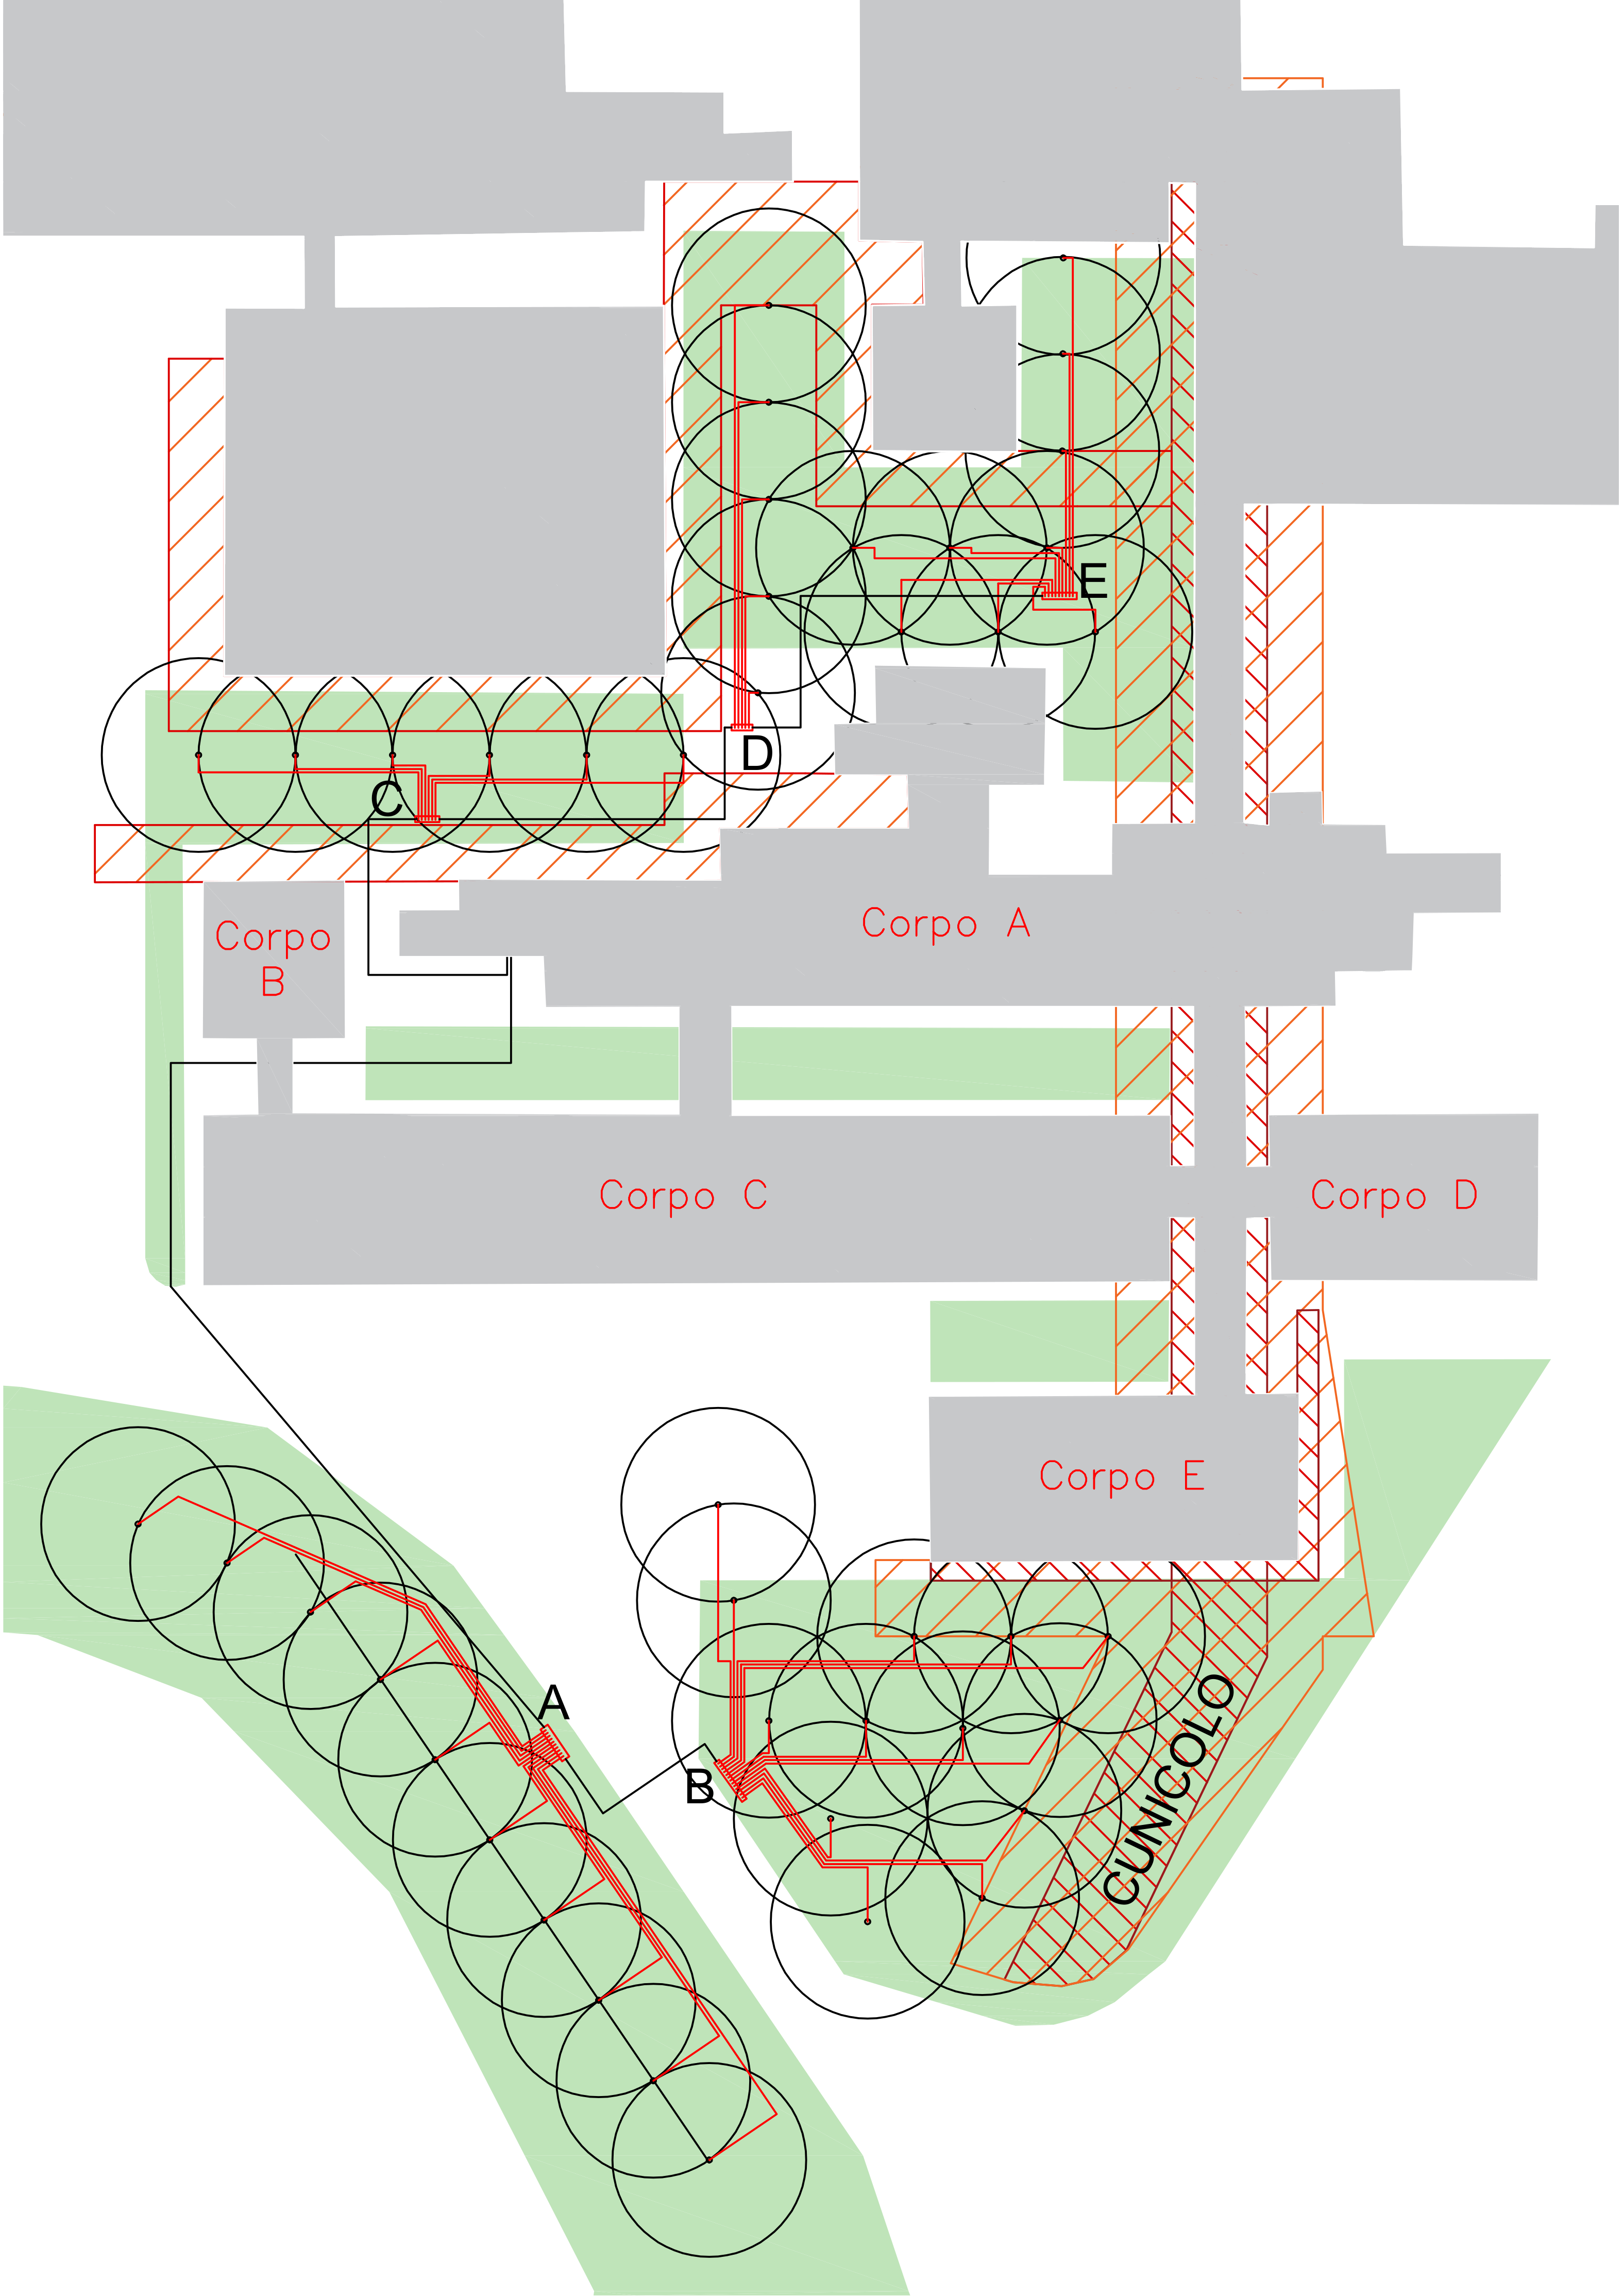
\includepdf{6_4_cap/img/geot}
\begin{figure}
	\centering
	\includegraphics[width=\hsize]{6_4_cap/img/geot}
	\caption{Disposizione sonde geotermiche intorno all'edificio 2}
	\label{img:geot}
\end{figure}

Nella sottocentrale sono state utilizzate, quindi, due pompe di calore in parallelo capaci di rendere in inverno \n{90}{kW} e \n{100}{kW} in estate: questa scelta è stata effettuata in quanto in caso di carico massimo le due macchine riescono a sfruttare tutto il campo geotermico mentre in occasione dei carichi parziali, è possibile spegnerne una e lavorare sempre a pieno carico (e quindi col massimo dell'efficienza). Vista la numerosa dotazione di macchine per il freddo, avere due pompe di calore permette di aumentare l'affidabilità del sistema geotermico.
\subsubsection{Gli scambiatori}
Come nel caso dell'acqua calda, gli scambiatori raffreddano l'acqua sfruttando la rete di presidio di acqua refrigerata. Gli scambiatori rappresentano \emph{l'ultima spiaggia} in caso di malfunzionamenti del gruppo ad assorbimento e delle pompe di calore.

Essendo l'ultimo \emph{strumento} disponibile in sottocentrale per \emph{il freddo}, si è deciso di dimensionare la coppia di scambiatori sul massimo carico estivo tenendo conto del solito coefficiente di sicurezza del \n{20}{\%} e di futuri ampliamenti. Quindi essendo $\dot{Q}_{\mathrm{frigo}}= \SI{730}{kW}$ la coppia di scambiatori avrà una potenzialità complessiva di \n{1}{MW} (ovvero ognuno è da \n{500}{kW}).

\vspace{1em}

Dopo aver spiegato come viene prodotto il \emph{caldo} e il \emph{freddo} in sottocentrale, è necessario descrivere brevemente la logica di funzionamento.

Per quanto riguarda la stagione invernale, le utenze che necessitano di acqua calda sono i radiatori, le batterie delle UTA, i fancoil e i bollitori per l'acqua calda sanitaria. Quindi avremo funzionanti gli scambiatori, per la produzione di acqua a \n{80}{\degreeCelsius} (per i radiatori e le batterie delle UTA), e le pompe di calore che andranno a produrre acqua a \n{50}{\degreeCelsius} per i fancoil. Per l'acqua calda sanitaria vengono usati i bollitori che sfruttano l'acqua surriscaldata proveniente direttamente dalla centrale. Nel caso in cui la temperatura esterna sia particolarmente estrema, entra in funzione un ulteriore scambiatore che produce acqua calda a \n{50}{\degreeCelsius} per i fancoil utilizzando l'acqua calda a \n{80}{\degreeCelsius} prodotta dai due scambiatori. Quest'ultimo scambiatore per i fancoil è stato dimensionato sulla potenza sensibile invernale dei due corpi maggiorato di un \n{20}{\%} per sicurezza e per tenere in considerazione di eventuali ampliamenti. La potenzialità risultante è pari a \n{100}{kW}. 

Nel caso estivo, invece, l'acqua refrigerata servirà ai fancoil e alle batterie di raffreddamento delle UTA mentre a quelle di post-riscaldamento servirà l'acqua calda. Pertanto funzioneranno sicuramente gli scambiatori per produrre acqua calda a \n{80}{\degreeCelsius} che verrà poi opportunamente miscelata con quella di ritorno più fredda per produrre acqua a \n{60}{\degreeCelsius} per le UTA; le pompe di calore e il gruppo ad assorbimento si occuperanno dell'acqua refrigerata. In questo modo la produzione del freddo risulterà a ``costo zero'' in quanto si usano i reflui termici (senza considerare ovviamente il consumo di energia elettrica per le pompe e il sistema di monitoraggio) prodotti dal cogeneratore e il campo geotermico come pozzo energetico.

In \vref{img:sott} si riporta lo schema della sottocentrale.

%\includepdf{6_4_cap/img/sottocentr}
\begin{figure}
	\centering
	\includegraphics[width=\textwidth]{6_4_cap/img/sottocentr}
	\caption{Schema Sottocentrale -- Edificio 2}
	\label{img:sott}
\end{figure}

	\chapter{Conclusioni}
\thispagestyle{empty}
Tutti gli interventi ipotizzati in questa analisi progettuale di riqualificazione energetica hanno prodotto dei risultati incoraggianti in quanto, come si è visto, è possibile ridurre in maniera molto più che evidente il consumo istantaneo di metano nella centrale di cogenerazione del policlinico necessario alla produzione di energia termica (sia per il \emph{caldo} che per il \emph{freddo}).

Dopo aver analizzato i carichi dello stato di fatto e di progetto è stata dimensionata la sottocentrale termica da costruirsi nel piano \num{-1} dell'edificio 2. 

L'ulteriore analisi effettuata è quella della \emph{certificazione energetica} in cui si è andato a valutare l'energia consumata all'interno dell'edificio 2 secondo la normativa UNI TS-11300. Questa verifica è stata eseguita, ovviamente, sia sullo stato di fatto che su quello di progetto.

Il software utilizzato appartiene alla suite \emph{CYPE}: \textbf{CYPETHERMUS C.E.}

In questo applicativo è stato importato il file \textsc{.ifc} e le stratigrafie dell'involucro (sia opaco che trasparente). Le zone termiche sono quelle utilizzate in fase di analisi dei carichi termici. Contestualmente sono stati inseriti i servizi energetici presenti all'interno dell'edificio 2:
\begin{itemize}
	\item Produzione di Acqua Calda Sanitaria;
	\item Riscaldamento;
	\item Raffrescamento;
	\item Ventilazione;
	\item Trasporto di persone/cose;
	\item Illuminazione.
\end{itemize}
Nello stato di fatto il riscaldamento/raffrescamento per UTIC, Emodinamica e il Blocco Operatorio avviene tramite un impianto a tutt'aria (che quindi assicura anche la ventilazione meccanica degli ambienti); per i corpi A e C non vi è il raffrescamento mentre il riscaldamento è assicurato dall'impianto con radiatori; la ventilazione in questi due corpi, invece, è di tipo naturale con un ricambio orario di \n{1}{vol/h}; per il servizio di trasporto è stato inserito un ascensore per il corpo A e le tre unità operatorie; l'illuminazione è stata valutata inserendo la potenzialità per \si{m^2} come indicato in fase di definizione dei locali.

I risultati presenti nell'\emph{Attestato di Prestazione Energetica degli edifici} (conosciuta anche come \emph{APE}) riferita allo stato di fatto, sono riassunti in \vref{ape:fatto}.
\begin{table}
	\centering
	\begin{tabular}{lccc}
		\toprule
		\multicolumn{4}{c}{{\large Stato di fatto}}\\
		\midrule
		\multirow{2}{*}{Superficie Utile}		 	& Heating & \num{4934.99} & \si{m^2}	\\
													& Cooling & \num{1152.49}  & \si{m^2} 	\\
		\multirow{2}{*}{Volume Lordo}				& Heating & \num{17768.49}& \si{m^3} 	\\
													& Cooling & \num{4185.23} & \si{m^3}    \\
		\multirow{2}{*}{Prestazione energetica fabbricato} 		& Heating 	  &	\multicolumn{2}{c}{\textbf{BASSA}}  \\
															  	& Cooling	  & \multicolumn{2}{c}{\textbf{BASSA}}  \\
		$\mathrm{EP_{gl,nren}}$	& \num{321.63}	& \multicolumn{2}{c}{\si{\frac{kWh}{m^2anno}}} \\
		Classe Energetica		&	\textbf{E} & &   \\
		$\mathrm{EP_{h,nd}}$	& \num{352.13}	& \multicolumn{2}{c}{\si{\frac{kWh}{m^2anno}}} \\
		Rapporto S/V			&	\num{0.40} &	&  \\
		$\mathrm{A_{sol,est}/A_{sol,utile}}$	&	\num{0.18} &	&  \\
		$\mathrm{Y_{IE}}$	&	\num{1.36}	& \multicolumn{2}{c}{\si{\frac{W}{m^2K}}}  \\
		\midrule
		\multicolumn{4}{c}{Fonti Energetiche Utilizzate}\\
		\midrule
		\multicolumn{2}{l}{Energia Elettrica da rete} 	& \num{320255.33} 	& \si{kWh} \\
		\multicolumn{2}{l}{Gas Naturale}			  	& \num{97024.34}		& \si{m^3} \\
		\bottomrule
	\end{tabular}
\caption{Prestazione Energetica -- Stato di fatto}\label{ape:fatto}
\end{table}
Le \emph{prestazioni energetiche} del fabbricato hanno restituito valori bassi, ovviamente. Per quanto riguarda la stagione invernale, il limite viene imposto dall'\emph{indice di prestazione termica utile} per il riscaldamento dell'edificio di riferimento. Nel caso, invece, della prestazione energetica estiva dell'involucro, l'indicatore è definito in base alla trasmittanza termica periodica $\mathrm{Y_{IE}}$ e all'area solare equivalente estiva per unità di superficie utile $\mathrm{A_{sol,est}/A_{sol,utile}}$. Per avere un risultato \textbf{ALTO}:
\begin{itemize}
	\item $\mathrm{A_{sol,est}/A_{sol,utile}} < \num{0.03}$;
	\item $\mathrm{Y_{IE}} < \num{0.14}$.
\end{itemize}

Le fonti energetiche utilizzate sono soltanto il \emph{Gas Naturale}, per il cogeneratore della centrale termica del policlinico, e l'\emph{Energia Elettrica} per il funzionamento degli ausiliari, illuminazione e trasporto.

Nello stato di progetto, invece, i risultati dell'APE sono riassunti in tabella \vref{ape:progetto}.

\begin{table}
	\centering
	\begin{tabular}{lccc}
		\toprule
		\multicolumn{4}{c}{{\large Stato di progetto}}\\
		\midrule
		\multirow{2}{*}{Superficie Utile}		 	& Heating & \num{4934.99} & \si{m^2}	\\
													& Cooling & \num{4934.99}  & \si{m^2} 	\\
		\multirow{2}{*}{Volume Lordo}				& Heating & \num{17768.49}& \si{m^3} 	\\
													& Cooling & \num{17768.49} & \si{m^3}    \\
		\multirow{2}{*}{Prestazione energetica fabbricato} 		& Heating 	  &	\multicolumn{2}{c}{\textbf{ALTA}}  \\
																& Cooling	  & \multicolumn{2}{c}{\textbf{BASSA}}  \\
		$\mathrm{EP_{gl,nren}}$	& \num{154.21}	& \multicolumn{2}{c}{\si{\frac{kWh}{m^2anno}}} \\
		Classe Energetica		&	\textbf{B} & &   \\
		$\mathrm{EP_{h,nd}}$	& \num{182.85}	& \multicolumn{2}{c}{\si{\frac{kWh}{m^2anno}}} \\
		Rapporto S/V			&	\num{0.40} &	&  \\
		$\mathrm{A_{sol,est}/A_{sol,utile}}$	&	\num{0.07} &	&  \\
		$\mathrm{Y_{IE}}$	&	\num{0.62}	& \multicolumn{2}{c}{\si{\frac{W}{m^2K}}}  \\
		\midrule
		\multicolumn{4}{c}{Fonti Energetiche Utilizzate}\\
		\midrule
		\multicolumn{2}{l}{Energia Elettrica da rete} 	& \num{235374.05}	 	& \si{kWh} \\
		\multicolumn{2}{l}{Gas Naturale}			  	& \num{30443.21}		& \si{m^3} \\
		\bottomrule
	\end{tabular}
\caption{Prestazione Energetica -- Stato di progetto}\label{ape:progetto}
\end{table}
Le differenze maggiori si hanno sul risparmio annuo delle fonti energetiche utilizzate. La motivazione risiede sia nelle migliori condizioni dell'involucro e sia nell'utilizzo di fonti rinnovabili (quale è la geotermia). L'intervento di \emph{relamping} ha, inoltre, contribuito alla diminuzione del consumo di energia elettrica. È, però, il decremento di gas naturale a saltare all'occhio in quanto se da una parte viene migliorato l'involucro (e quindi è necessario riscaldare meno come lo si evince dal $\mathrm{EP_{h,nd}}$ che risulta essere molto più basso rispetto al corrispettivo valore dello stato di fatto), dall'altro vengono usate le pompe di calore che sfruttano il calore endogeno del terreno antistante l'edificio 2.

Essendo l'edificio oggetto di intervento sottoposto ad una \emph{riqualificazione energetica}, i \emph{requisiti minimi}\footnote{dal DM 16/6/15} che sono stati verificati sono:
\begin{itemize}
	\item trasmittanze opache e trasparenti inferiori ai valori limiti indicati (come in \vref{vallim:opve});
	\item trasmittanze dei divisori tra edifici o unità immobiliari distinti inferiori a~\n{0.8}{\trasm};
	\item altezze minime dei locali di abitazione derogate fino a un massimo di \n{10}{cm};
	\item assenza di rischio di formazione di muffe (con particolare attenzione ai ponti termici) e di condensazione interstiziale;
	\item la riflettanza per le strutture di copertura piane superiore a \num{0.65};
	\item il valore del fattore di trasmissione solare totale delle chiusure trasparenti $\mathrm{g_{gl+sh}<0.35}$;
	\item installazione di opportuni dispositivi per la regolazione automatica per singolo ambiente o per singola unità immobiliare, assistita da compensazione climatica.
\end{itemize}
È interessante notare come per una riqualificazione energetica non sia necessario considerare l'inerzia dell'involucro opaco per contenere il carico estivo.

Ritornando ai risultati ottenuti, considerando che l'AOU ``Federico II'' compra da \emph{Studium Power\&Service} (che possiede tutta la centrale termofrigorifera) energia elettrica e termica è possibile valutare il risparmio annuale che si ottiene effettuando gli interventi ipotizzati in questo elaborato di laurea.

Si riportano i prezzi unitari offerti al policlinico: 
\begin{itemize}
	\item Energia elettrica: \num{0.114}\ \euro/kWh;
	\item Energia termica: \num{0.057}\ \euro/kWh.
\end{itemize}
Il risparmio annuale sarà, quindi:
\begin{itemize}
	\item \num{17778}\ \euro\- di energia termica; %0.267 euro/mc di gas
	\item \num{9676}\ \euro\- di energia elettrica.
\end{itemize}

Ad un risparmio energetico ne è sempre affiancato uno sugli agenti inquinanti immessi in atmosfera: utilizzare meno energia implica, per come è costruita la filiera energetica italiana (e mondiale), introdurre in ambiente meno inquinanti. 

Pertanto i risultati sono i seguenti:
\begin{itemize}
	\item \n{54.93}{tep}; % 1 mc di gas equivale a 8250x10-7
	\item \num{23.8}\ tonnellate equivalenti di $\mathrm{CO_2}$ % 1 ton di CO2 equivale a 2.30 tep
\end{itemize}

I risultati sono molto incoraggianti: è possibile risparmiare in bolletta annualmente quasi \num{30000}\ \euro. Considerando che il budget per coprire le spese deriva dal \emph{Fondo per lo sviluppo e la coesione 2014-2020}, il policlinico può trarre, quindi, solo un grande vantaggio. A lavori ultimati, l'AOU possederà un edificio in classe B con tutte le conseguenze che ne derivano: involucro capace di resistere sia alla stagione invernale che quella estiva; un impianto idronico, aeraulico e elettrico moderno monitorato da un adeguato sistema di contabilizzazione dell'energia e di individuazione di eventuali guasti. Il tutto si traduce in maggior comfort per i degenti nonché per i medici, infermieri e studenti che occupano e vivono l'edificio.
	%\chapter{Glossario}
tyhdtgrsfe
	\backmatter
	\addcontentsline{toc}{chapter}{\bibname} 
\begin{thebibliography}{9}
	\bibitem{beguinot}Ing. Beguinot, Corrado, \emph{Ospedali e Cliniche Universitarie -- \emph{III Volume}}
	\bibitem{alfano}Alfano, Filippi, Sacchi, \emph{Impianti di Climatizzazione per l'Edilizia}
	\bibitem{delmastro}Del Mastro, Noce, \emph{GSHP -- \emph{Geotermia a sonde verticali}}
	\bibitem{palombo}Palombo, Adolfo, \emph{Impianti di Climatizzazione}
	\bibitem{12831} UNI EN 12831, \emph{Impianti di riscaldamento negli edifici -- \emph{Metodo di calcolo del carico termico di progetto}}
	\bibitem{9182} UNI 9182, \emph{Impianti di alimentazione e distribuzione d'acqua fredda e calda}
	\bibitem{10339} UNI 10339, \emph{Impianti aeraulici al fini di benessere}
\end{thebibliography}
\thispagestyle{empty}
	\addcontentsline{toc}{chapter}{Elenco delle figure} 
\listoffigures
\thispagestyle{empty}
	\addcontentsline{toc}{chapter}{Elenco delle tabelle} 
\listoftables
\thispagestyle{empty}
	\thispagestyle{empty}
\mbox{}

\newpage
\thispagestyle{empty}
\vspace*{5cm}
\begin{changemargin}{0.5cm}{0.5cm}
	\noindent
	Lo studio presente in questo elaborato di laurea ha permesso sia di affacciarmi in prima persona al mondo del lavoro (ovvero applicare la teoria appresa all'università), sia di interfacciarmi con la macchina burocratica e con tutto quell'apparato di normative e leggi che, da una parte, consigliano e promuovono la \emph{retta via}, dall'altra, limitano e avviliscono l'operato umano privilegiando la mediocrità senza incoraggiare, invece, l'ingegno e la creatività che contraddistinguono un essere umano dall'altro.
	
	\vspace{1em}\noindent
	Consapevole di dovermi un giorno scontrare con poteri e logiche più forti di me, spero e mi
	auguro di avere sempre la forza di seguire le parole di \emph{Baden Powell}, fondatore dello scoutismo: ``\emph{Procurate di lasciare il mondo un po' migliore di come lo avete trovato}''.
	\vspace{1em}
\end{changemargin}

\newpage
\thispagestyle{empty}
\vspace*{8cm}
\centering\large Leave the world a little better than you found it\\\vspace{0.2em}{\hspace{5cm}\normalsize --- Baden Powell}
\end{document}